\documentclass[a4paper]{report}
\usepackage[T1]{fontenc}
\usepackage[utf8]{inputenc}
\usepackage[italian]{babel} 
\usepackage{amsfonts} %matematica
\usepackage{amsmath} %matematica
\usepackage{amssymb} %simboli matematica
\usepackage{amsthm} %teoremi matematici
\usepackage{tikz}

\usepackage{matlab-prettifier}

\theoremstyle{definition}
\newtheorem*{Esercizio}{Esercizio}
\newtheorem*{Definizione}{Definizione}
\newtheorem*{Proposizione}{Proposizione}

\usepackage{booktabs} %tabelle
\usepackage{graphicx} %figure
\usepackage{capt-of} %caption
\graphicspath{{Immagini/}} %percorso delle figure

\title{Robotica Industriale}
\author{Angelo D'Amante}
\date{A.A. 2018/2019}

\begin{document}
\maketitle
\tableofcontents

\chapter{Cinematica dei Robot}

\paragraph{}
In questo capitolo esploriamo la cinematica dei manipolatori robotici, i metodi per la rappresentazione dell'orientazione possono essere di due tipi: ridondanti e minimi.

\paragraph{}
Esempi di rappresentazioni minime: 
\begin{itemize}
\item angoli di Eulero ZYZ
\item angoli roll, pitch, yaw (rollio, beccheggio e imbardata)
\end{itemize}

\paragraph{}
Esempi di rappresentazioni ridondanti:
\begin{itemize}
	\item matrici di rotazione (9 numeri)
	\item quaternione unitario
\end{itemize}

\paragraph{}
Le rappresentazioni ridondanti si usano perchè evitano le singolarità algebriche, inevitabili usando le rappresentazioni minime.

\paragraph{}
Prima di iniziare, poniamo attenzione alla notazione: con $\underline{Q}$ indichiamo un vettore colonna di $\mathbb{R}^{n}$ e con una lettera maiuscola, come $A$ indichiamo una matrice.

\section{Matrici di Rotazione}

\paragraph{}
Scegliamo due terne cartesiane ortogonali $\langle0\rangle$, $\langle1\rangle$ ad origini distinte.\\

%due SdR, uno inerziale
\begin{tikzpicture} [y ={(1 cm ,0 cm )}, x ={( -0.5 cm , -0.5 cm )}, z ={(0 cm ,1 cm )}]
	\coordinate (0) at (0,0,0);
	\draw[->] (0)--(2,0,0) node [left] {$x_{0}$};
	\draw[->] (0)--(0,2,0) node [right] {$y_{0}$};
	\draw[->] (0)--(0,0,2) node [above] {$z_{0}$};
	\node[anchor = north] (0) at (0) {$O_{0}$};

	\coordinate (O1) at (0,6,0);
	\draw[->] (O1)--(2,6,0) node [left] {$x_{1}$};
	\draw[->] (O1)--(0,8,1) node [right] {$y_{1}$};
	\draw[->] (O1)--(0,5,2) node [above] {$z_{1}$};
	\node[anchor = north] (O1) at (O1) {$O_{1}$};
\end{tikzpicture}

\paragraph{}
Possiamo considerare $O_{0}$ e $O_{1}$ coincidenti, senza perdere di generalità. \\
Identifichiamo $\vec{i_{0}}$, $\vec{j_{0}}$, $\vec{k_{0}}$, $\vec{i_{1}}$, $\vec{j_{1}}$, $\vec{k_{1}}$ come i versori delle due terne. 
\paragraph{}
Adesso definiamo $\underline{^0i_{0}} \in \mathbb{R}^{3}$ come il vettore contenente le componenti di $\vec{i_{0}}$ in terna $\langle0\rangle$. Quindi, otteniamo:

\[\underline{^0i_{0}} = \begin{bmatrix}1\\0\\0\end{bmatrix}\]e il vettore $\underline{^0i_{1}}$ esprimibile come:
$\underline{^0i_{1}} = i_{1x}\cdot\underline{i} + i_{1y}\cdot\underline{j} + i_{1z}\cdot\underline{k}$

Nella terna $\langle0\rangle$ vale: $\underline{^0i_{0}} = \underline{i}, \, \underline{^0j_{0}} = \underline{j},\, \underline{^0k_{0}} = \underline{k}$ per evitare l'abuso di notazione.

\paragraph{}
Esprimendo i versori della terna $\langle1\rangle$ in terna $\langle0\rangle$, otteniamo:\\
\begin{equation}
	\begin{cases}
		\underline{^0i_{1}}=i_{1x}\cdot\underline{i} + i_{1y}\cdot\underline{j} + i_{1z}\cdot\underline{k}\\
		\underline{^0j_{1}}=j_{1x}\cdot\underline{i} + j_{1y}\cdot\underline{j} + j_{1z}\cdot\underline{k}\\
		\underline{^0k_{1}}=k_{1x}\cdot\underline{i} + k_{1y}\cdot\underline{j} + k_{1z}\cdot\underline{k}\\
	\end{cases}
\end{equation}
possiamo organizzare i 9 numeri in una matrice $3x3$ che battezziamo \emph{Matrice di Rotazione}, detta anche matrice dei coseni direttori:

%matrice di Rotazione
\begin{equation}
	R_{1}^{0} = 
	\begin{bmatrix}
		i_{1x} & j_{1x} & k_{1x} \\
		i_{1y} & j_{1y} & k_{1y} \\
		i_{1z} & j_{1z} & k_{1z} \\
	\end{bmatrix}
	= 
	\begin{bmatrix}
		\:\underline{^0i_{1}} \quad \underline{^0j_{1}} \quad\underline{^0k_{1}}\:
	\end{bmatrix}
\end{equation}

\subsection{Codifica l'orientazione}
\paragraph{}
La prima utilità di $R_{1}^{0}$ è quella di codificare l'orientazione relativa di $\langle1\rangle$ rispetto a $\langle0\rangle$, attraverso i versori di $\langle1\rangle$ espressi in terna $\langle0\rangle$.

\subparagraph{Espressione di $R_{1}^{0}$ per rotazione attorno all'asse $z$}
\paragraph{}%SdR pg 3
\begin{figure}[ht]
	\begin{minipage}[b]{0.45\linewidth}
		\centering
		\begin{tikzpicture}[y ={(0 cm ,1 cm )}, x ={( 1 cm , 0 cm )}]
			\coordinate (O) at (0,0);
			\draw[->] (O)--(2,0) node [right] {$x_{0}$};
			\draw[->] (O)--(0,2) node [above] {$y_{0}$};
			\draw  (O) circle [ radius = 0.1 cm] node [below] {$z_{0}\equiv z_{1}$};
			\draw[->, color = red] (O)--(2,1) node [right] {$x_{1}$};
			\draw[help lines, ->] (O)--(1,0.5) node [above] {$\underline{i_{1}}$};
			\draw[->, color = red] (O)--(-1,2) node [above] {$y_{1}$};
			\draw[help lines, ->] (O)--(-0.5,1) node [left] {$\underline{j_{1}}$};
			\draw [->] (1,0) arc(0:30:1);
			\node at (1.2cm, 0.3cm) {$\theta$};
			\draw [->] (0,1) arc(90:120:1);
			\node [above] at (-0.3cm, 1cm) {$\theta$};
		\end{tikzpicture}
	\end{minipage}
	\begin{minipage}[b]{0.45\linewidth}
		\centering
		\begin{equation*}
			R_{1}^{0} = 
			\begin{bmatrix}
				\cos(\theta) & -\sin(\theta) & 0 \\
				\sin(\theta) & \cos(\theta) & 0 \\
				0 & 0 & 1 \\
			\end{bmatrix}
		\end{equation*}
	\end{minipage}
\end{figure}
\newpage %interruzione di pagina

\subparagraph{Espressione di $R_{1}^{0}$ per rotazione attorno all'asse $x$}
\paragraph{}%SdR pg 3
\begin{figure}[ht]
	\begin{minipage}[b]{0.45\linewidth}
		\centering
		\begin{tikzpicture}[y ={(0 cm ,1 cm )}, x ={( 1 cm , 0 cm )}]
			\coordinate (O) at (0,0);
			\draw[->] (O)--(2,0) node [right] {$y_{0}$};
			\draw[->] (O)--(0,2) node [above] {$z_{0}$};
			\draw  (O) circle [ radius = 0.1 cm] node [below] {$x_{0}\equiv x_{1}$};
			\draw[->, color = red] (O)--(2,1) node [right] {$y_{1}$};
			\draw[help lines, ->] (O)--(1,0.5) node [above] {$\underline{j_{1}}$};
			\draw[->, color = red] (O)--(-1,2) node [above] {$z_{1}$};
			\draw[help lines, ->] (O)--(-0.5,1) node [left] {$\underline{k_{1}}$};
			\draw [->] (1,0) arc(0:30:1);
			\node at (1.2cm, 0.3cm) {$\theta$};
			\draw [->] (0,1) arc(90:120:1);
			\node [above] at (-0.3cm, 1cm) {$\theta$};
		\end{tikzpicture}
	\end{minipage}
	\begin{minipage}[b]{0.45\linewidth}
		\centering
		\begin{equation*}
			R_{1}^{0} = 
			\begin{bmatrix}
				1 & 0 & 0 \\
				0 & \cos(\theta) & -\sin(\theta) \\
				0 & \sin(\theta) & \cos(\theta) \\
			\end{bmatrix}
		\end{equation*}
	\end{minipage}
\end{figure}

\subparagraph{Espressione di $R_{1}^{0}$ per rotazione attorno all'asse $y$}
\paragraph{}%SdR pg 3
\begin{figure}[ht]
	\begin{minipage}[b]{0.45\linewidth}
		\centering
		\begin{tikzpicture}[y ={(0 cm ,1 cm )}, x ={( 1 cm , 0 cm )}]
			\coordinate (O) at (0,0);
			\draw[->] (O)--(2,0) node [right] {$z_{0}$};
			\draw[->] (O)--(0,2) node [above] {$x_{0}$};
			\draw  (O) circle [ radius = 0.1 cm] node [below] {$y_{0}\equiv y_{1}$};
			\draw[->, color = red] (O)--(2,1) node [right] {$z_{1}$};
			\draw[help lines, ->] (O)--(1,0.5) node [above] {$\underline{k_{1}}$};
			\draw[->, color = red] (O)--(-1,2) node [above] {$x_{1}$};
			\draw[help lines, ->] (O)--(-0.5,1) node [left] {$\underline{i_{1}}$};
			\draw [->] (1,0) arc(0:30:1);
			\node at (1.2cm, 0.3cm) {$\theta$};
			\draw [->] (0,1) arc(90:120:1);
			\node [above] at (-0.3cm, 1cm) {$\theta$};
		\end{tikzpicture}
	\end{minipage}
	\begin{minipage}[b]{0.45\linewidth}
		\centering
		\begin{equation*}
			R_{1}^{0} = 
			\begin{bmatrix}
				\cos(\theta) & 0 & \sin(\theta) \\
				0 & 1 & 0 \\
				-\sin(\theta) & 0 & \cos(\theta) \\
			\end{bmatrix}
		\end{equation*}
	\end{minipage}
\end{figure}

\paragraph{}
Notiamo che in generale il $\det(R_{1}^{0}) = 1 $, quindi $R_{1}^{0}$ è invertibile, ma solo se parliamo di rotazione sinistrorsa (o levogira). Infatti, nel caso la matrice $R_{1}^{0}$ sia destrorsa allora si ha che $\det(R_{1}^{0}) = -1 $.

\subsection{Cambio di coordinate di un punto dello spazio}

\paragraph{}
Usiamo la matrice $R$ per cambiare le coordinate di un punto dello spazio tra terne ad origine comune. 


\paragraph{}
\begin{center}
	\begin{tikzpicture}[y ={(1cm, 0cm)}, x ={(-0.5cm, -0.5cm)}, z ={(0 cm, 1 cm)}]
		\coordinate (O) at (0,0,0);
		\draw[->] (O) -- (0,2,0) node [right] {$y_{0}$};
		\draw[->] (O) -- (0,0,2) node [above] {$z_{0}$};
		\draw[->] (O) -- (2.5,0,0) node [right] {$x_{0}$};

		\draw[->, gray] (O) -- (0,2,1) node [right] {$y_{1}$};
		\draw[->, gray] (O) -- (0,-1,2) node [above] {$z_{1}$};
		\draw[->, gray] (O) -- (2.5,1.2,0) node [right] {$x_{1}$};
	
		\node (P) at (0,2,2) {$\underline{P}$};
		\draw[->, blue] (O) -- (P);
	\end{tikzpicture}
\end{center}

$\vec{O_{o}P}$ possiamo esprimerlo in terna $\langle 0 \rangle$ oppure in terna $\langle 1 \rangle$. Ovvero: 

$\underline{^{0}P} = 
	\begin{bmatrix}
		p_{0x} & p_{0y} & p_{0z}
	\end{bmatrix}^{T}\quad$
e 
$\quad\underline{^{1}P} = 
	\begin{bmatrix}
		p_{1x} & p_{1y} & p_{1z}
	\end{bmatrix}^{T}$
	
\paragraph{}
Otteniamo: $p_{0x}\:\underline{i}+p_{0y}\:\underline{j}+p_{0z}\:\underline{k} = p_{1x}\:\underline{^0i_{1}}+p_{1y}\:\underline{^0j_{1}}+p_{1z}\:\underline{^0k_{1}}$ e ho quindi espresso $\underline{^0P}$ in due modi e allora posso riscrivere il vettore come segue: 

\begin{equation}
	\underline{^0P}=
	\begin{bmatrix}
		\;\underline{^0i_{1}} & \underline{^0j_{1}} & \underline{^0k_{1}}\;
	\end{bmatrix}
	\begin{bmatrix}
		p_{1x} \\
		p_{1y} \\
		p_{1z}
	\end{bmatrix}
	= R_{1}^{0} \: \underline{^1P}	
\end{equation}
Questa relazione non vale solo per i vettori posizione, ma anche per velocità, velocità angolari, forze, ecc...

\subsection{Proprietà di $R$}
\begin{itemize}
	\item $\det(R) = \vert R \vert = 1$
	\item $R^{\,-1} = R^{T}$
	\item $R^{T}R = I$
\end{itemize}
Quest'ultima proprietà si dimostra ponendo, 
\begin{equation*}
	R_1^0 =
	\begin{bmatrix}
		\:\underline{^0i_1} & \underline{^0j_1} & \underline{^0k_1}\:
	\end{bmatrix}
	= R
\end{equation*} e facendo il prodotto con la sua trasposta, ottengo:
\begin{equation*}
	R^{T} \cdot R =
	\begin{bmatrix}
		\:\underline{^0i_1}\: \\
		\:\underline{^0j_1}\: \\
		\:\underline{^0k_1} \:
	\end{bmatrix}
	\cdot
	\begin{bmatrix}
		\: \underline{^0i_1} & \underline{^0j_1} & \underline{^0k_1} \:
	\end{bmatrix}
	= 
	\begin{bmatrix}
		1 & 0 & 0 \\
		0 & 1 & 0 \\
		0 & 0 & 1 
	\end{bmatrix}
	= I_{3x3}
\end{equation*}

\subsection{Derivata temporale di $R$}
\paragraph{}
Per due terne $\langle 0 \rangle$, $\langle 1 \rangle$ in moto relativo tra loro, vale $R = R(t)$, senza perdere di generalità, supponiamo $O_0 = O_1$ e scegliamo un punto $\underline{P}$ fisso in terna $\langle 1 \rangle$. Deriviamo quindi $\underline{^0P} = R_{1}^{0} \cdot \underline{^1P}$ e otteniamo:

\begin{equation}
	\dfrac{d}{dt} \; (^0\underline{P}) = \underline{^0\dot{P}} = \dot{R_{1}^{0}}\; ^1\underline{P} + R_{1}^{0} \; ^1\underline{\dot{P}} = \dot{R_{1}^{0}}\; ^1\underline{P}
\end{equation}
Utilizzando la formula fondamentale dei moti rigidi 
\begin{equation}
	\underline{\dot{P}} = \underline{\dot{O_{1}}} + \underline{^0\omega_{1}} \times R_{1}^{0}\: \underline{^1P} = \underline{\dot{O_{1}}} + \underline{^0\omega_{1}} \times \: \underline{^0P}
\end{equation}
Uguagliando la (1.4) e la (1.5) otteniamo: 
\begin{equation}
	\dot{R_{1}^{0}}\;\underline{^1P} = \underline{^0\omega_{1}} \times ( R_{1}^{0} \; \underline{^1P}) = S(^0\omega_{1}) \; R_{1}^{0} \; \underline{^1P}
\end{equation} 
Isolando la matrice di rotazione otteniamo le \emph{Formule di Poisson} "condensate" in una sola matriciale:
\begin{equation}
	\dot{R_{1}^{0}} = S(^0\omega_{1}) \; R_{1}^{0} 
\end{equation}

\subparagraph{Notiamo la funzione $S(\cdot)$:}
Il prodotto vettoriale $ \underline{a} \times \underline{b} $ viene espresso mediante l'uso della funzione (\emph{formalismo matriciale}):
\begin{equation*}
	S(\underline{a}) = 
	\begin{bmatrix}
		0 & -a_z & a_y \\
		a_z & 0 & -a_x \\
		-a_y & a_x & 0
	\end{bmatrix}
\end{equation*}
e quindi risulta: $\underline{a} \times \underline{b} = S(\underline{a}) \; \underline{b}$ e inoltre notiamo la proprietà $S^T(\cdot) = - S(\cdot)$.

\section{Rotazioni nello spazio}
\paragraph{}
Consideriamo di \emph{ruotare un vettore nello spazio}, cioè andiamo a \emph{premoltiplicare} una certa matrice di rotazione $R$ per un vettore $\underline{v}$ dato. Noi abbiamo:
\begin{equation*}
	\underline{v} = \vert\underline{v}\vert \; 
	\begin{bmatrix}
		\cos(\alpha) \\
		\sin(\alpha) \\
		0
	\end{bmatrix}	
	\qquad
	R =
	\begin{bmatrix}
		\cos(\beta) & -\sin(\beta) & 0 \\
		\sin(\beta) & \cos(\beta) & 0 \\
		0 & 0 & 1
	\end{bmatrix}
\end{equation*}
e otteniamo $\underline{w}=R\,\underline{v}$, vediamo come è fatto $\underline{w}$:
\begin{align*}
	\underline{w} = 
	\begin{bmatrix}
		w_x \\
		w_y \\
		w_z
	\end{bmatrix}
	=
	\begin{bmatrix}
		\cos(\beta) & -\sin(\beta) & 0 \\
		\sin(\beta) & \cos(\beta) & 0 \\
		0 & 0 & 1
	\end{bmatrix}
	\begin{bmatrix}
		\cos(\alpha) \\
		\sin(\alpha) \\
		0
	\end{bmatrix}
	\vert\underline{v}\vert = \\
	=
	\begin{bmatrix}
		\cos(\alpha)\cos(\beta) - \sin(\alpha)\sin(\beta) \\
		\cos(\alpha)\sin(\beta) - \cos(\alpha)\sin(\beta) \\
		0
	\end{bmatrix}
	\vert\underline{v}\vert = 
	\begin{bmatrix}
		\cos(\alpha + \beta) \\
		\sin(\alpha + \beta) \\
		0
	\end{bmatrix}
	\vert\underline{v}\vert
\end{align*}
quindi, $\forall\underline{v}$ e $\forall R$ \emph{allora} $\underline{w} = R \underline{v}$ è un vettore con lo stesso modulo di $\underline{v}$ ruotato nello spazio, di un certo angolo ed attorno ad un certo asse, \emph{codificati in $R$}.

\paragraph{}
Possiamo fare delle \emph{rotazioni successive} nello spazio, e abbiamo due possibilità: 
\begin{itemize}
	\item composizione di rotazioni specificate in \emph{terna corrente}
	\item composizione di rotazioni specificate in \emph{terna fissa}
\end{itemize}

\subsection{Rotazioni in terna corrente}
\paragraph{}
Supponiamo di avere tre terne $\langle0\rangle$, $\langle1\rangle$, $\langle2\rangle$ ad origine comune ed un punto $\underline{P}$.

\begin{equation*}
	\begin{cases}
		^0\underline{P} = R_1^0 \, ^1\underline{P} \\
		^1\underline{P} = R_2^1 \, ^2\underline{P} \\
		^0\underline{P} = R_2^0 \, ^2\underline{P}
	\end{cases}
	\Rightarrow
	\begin{cases}
		^0\underline{P} = R_1^0 \, R_2^1 \, ^2\underline{P} \\
		^0\underline{P} = R_2^0 \, ^2\underline{P}
	\end{cases}
	\Rightarrow
	R_2^0 = R_1^0 \, R_2^1
\end{equation*}

Si generalizza a $n+1$ terne:  
\begin{equation}
	R_n^0 = R_1^0 \, R_2^1 \, \cdots R_{n-1}^{n-2} \, R_{n}^{n-1}
\end{equation}

ottenendo la \emph{Matrice che mappa la terna $n$ nella terna $0$}.
\newpage

\subsection{Rotazioni in terna fissa}
\paragraph{}
Supponiamo di avere tre terne $\langle0\rangle$, $\langle1\rangle$, $\langle2\rangle$ ad origine comune e che la terna $\langle 0 \rangle$ sia fissa. Quindi, definiamo:
\begin{itemize}
	\item $R_1^0$ trasforma i versori principali della terna $\langle 0 \rangle$ (espressi in $\langle 0 \rangle$) nei versori principali della terna $\langle 1 \rangle$ espressi in $\langle 0 \rangle$.
	\item $^0R_2^1$ trasforma i versori principali della terna $\langle 1 \rangle$ nei versori principali della terna $\langle 2 \rangle$ entrambi \emph{espressi in terna $\langle 0 \rangle$}.
\end{itemize}

Con la notazione appena introdotta è facile verificare che $R_1^0 \equiv \,^0R_1^0$.
\paragraph{}
Applichiamo $^0R_2^1$ ai versori di $\langle1\rangle$, otteniamo:
\begin{equation*}
	\begin{cases}
		^0\underline{i_2} = ^0R_2^1 \, ^0\underline{i_1} \\
		^0\underline{j_2} = ^0R_2^1 \, ^0\underline{j_1} \\
		^0\underline{k_2} = ^0R_2^1 \, ^0\underline{k_1}
	\end{cases}
	\Leftrightarrow
	\begin{bmatrix}
		^0\underline{i_2} & ^0\underline{j_2} & ^0\underline{k_2}
	\end{bmatrix}
	= \,^0R_2^1 \,
	\begin{bmatrix}
		^0\underline{i_1} & ^0\underline{j_1} & ^0\underline{k_1}
	\end{bmatrix}
\end{equation*}  

ovvero:
\begin{equation*}
	^0R_2^0 = \,^0R_2^1 \, ^0R_1^0
\end{equation*}

E generalizzando otteniamo la \emph{regola di composizione di rotazioni in terna fissa}:
\begin{equation}
	^0R_n^0 = \,^0R_n^{n-1} \cdot \,^0R_{n-1}^{n-2} \,  \cdots \, ^0R_{2}^{1} \cdot \,^0R_{1}^{0}
\end{equation}
Vediamo come calcolare $^0R_2^1$:

\begin{equation}
	\begin{cases}
		R_2^0 = R_1^0\,R_2^1 \\
		R_2^0 = \,^0R_2^1\,R_1^0 
	\end{cases}
	\Rightarrow
	R_1^0\,R_2^1 = \,^0R_2^1\,R_1^0 \;
	\Rightarrow \;
	^0R_2^1 = R_1^0\,R_2^1\,(R_1^0)^T
\end{equation}

ho espresso le due composizioni e ho moltiplicato per $(R_1^0)^T$.

\subsubsection{Non commutatività delle rotazioni}
Il prodotto matriciale non è commutativo, così come \emph{non} lo sono le rotazioni, vediamo infatti un esempio in terna corrente:

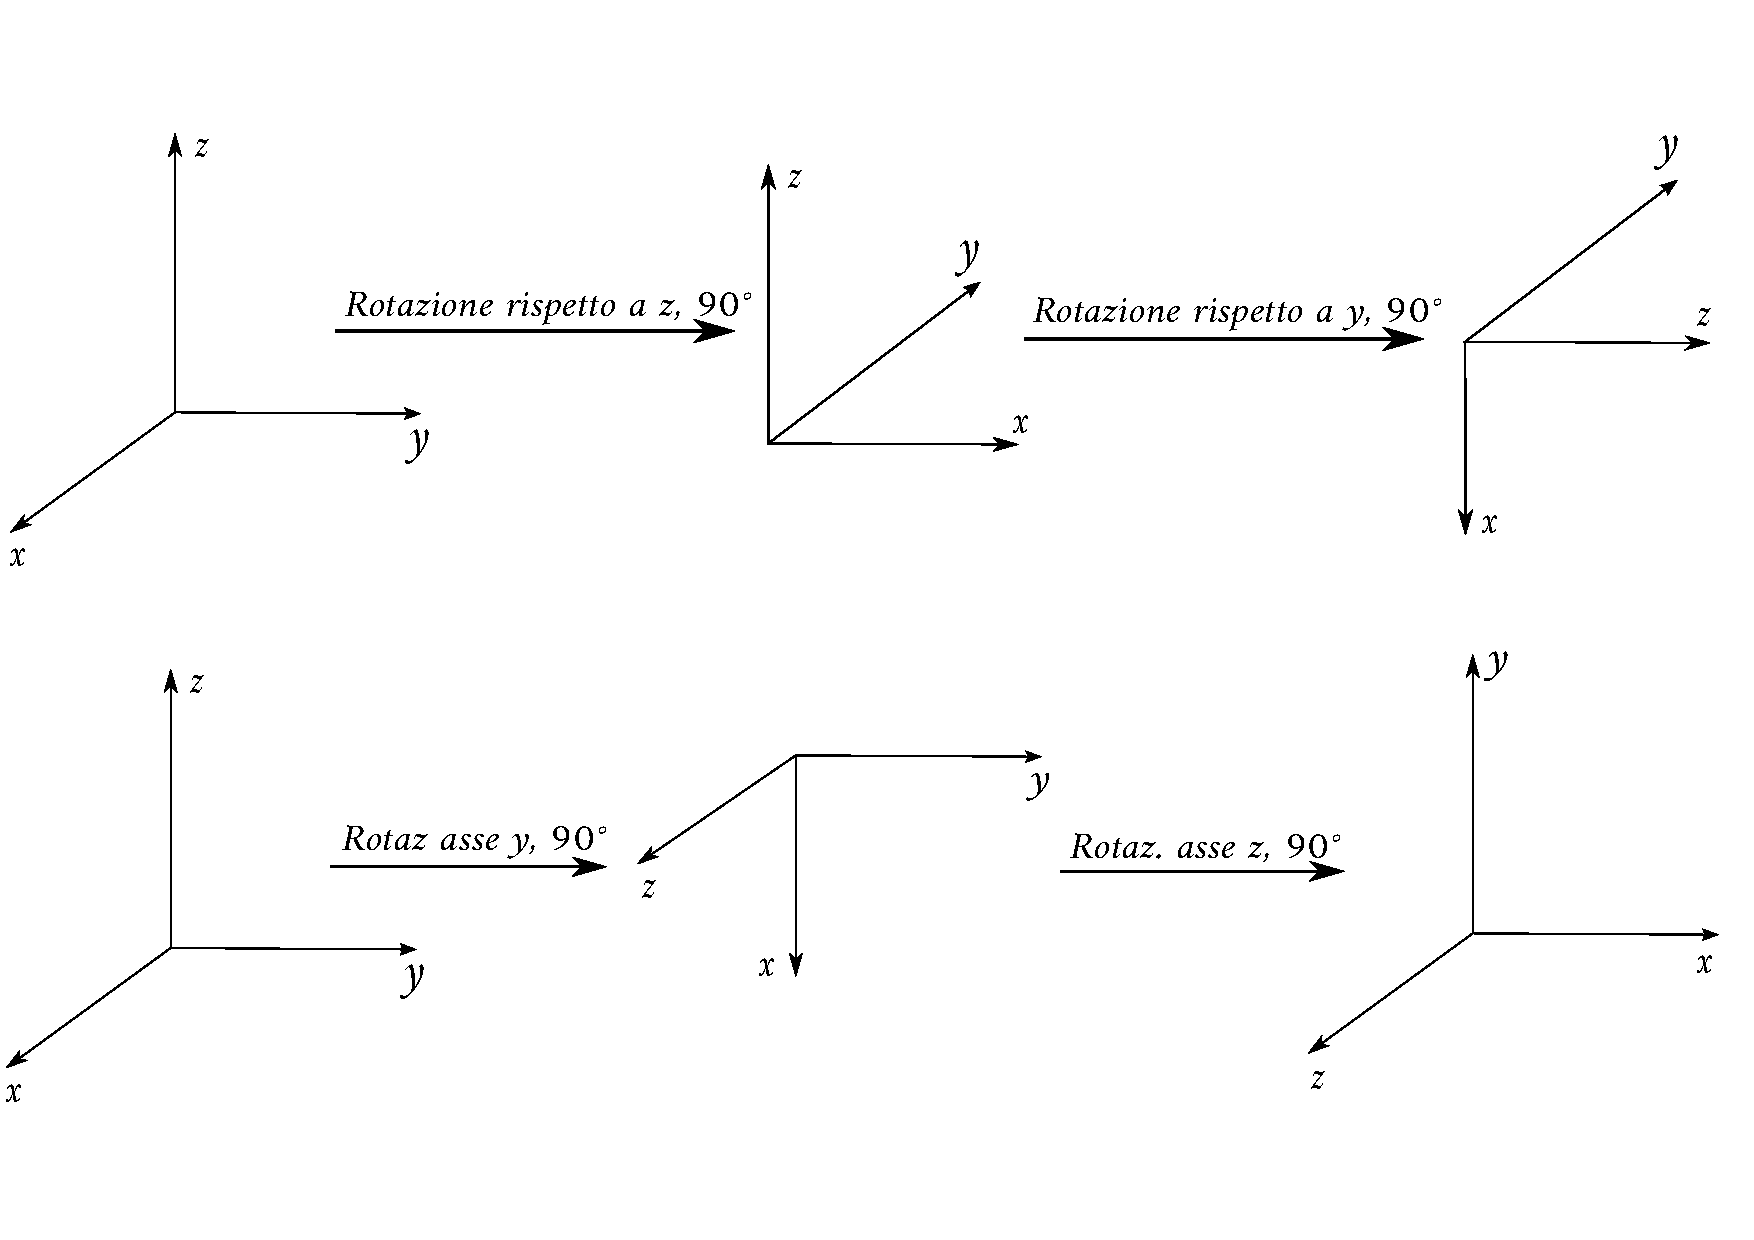
\includegraphics[scale=0.35]{rotazioniNonCommutative.pdf}
\newpage

\section{Rappresentazione Asse - Angolo}
Si parte dal ricavare la $R$ corrispondente ad una rotazione di $\theta$ (arbitrario) attorno ad un asse identificato da un versore $\underline{r}$ (arbitrario). $\underline{r}$ è univocamente determinato da $\alpha$ e $\beta$ e poi vedremo il contrario.

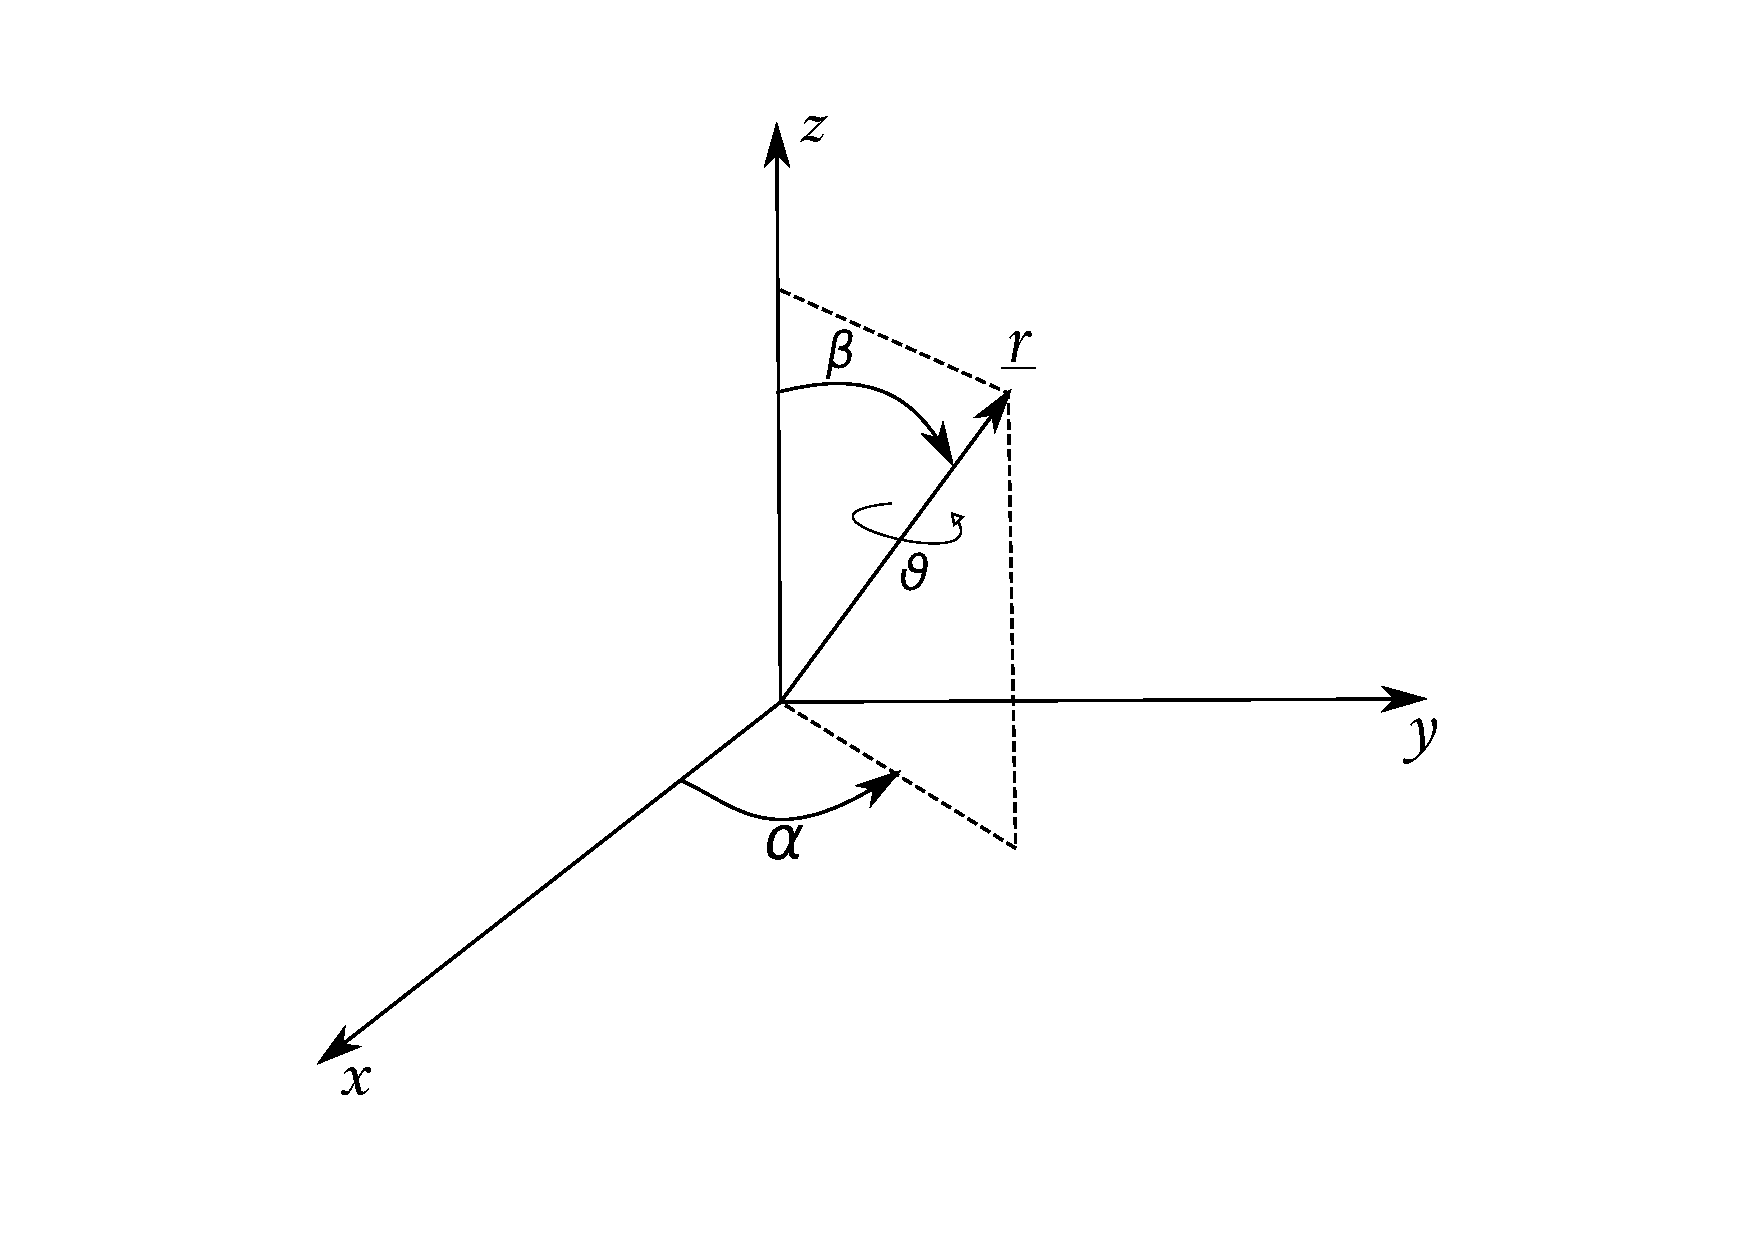
\includegraphics[scale=0.35]{asseAngolo.pdf}
\captionof{figure}{Rotazione di un angolo intorno ad un asse}

\subsection{Ricavare $R$ partendo da asse e angolo}
Dato che non sappiamo scrivere di getto $R_{\underline{r}}(\theta)$, otteniamola come \emph{successione di rotazioni specificate in terna fissa}:
\begin{enumerate}
	\item Attorno all'asse $z$ di $- \alpha$
	\item Attorno all'asse $y$ di $- \beta$
	\item Attorno all'asse $z$ di $\theta$ ($\Rightarrow rotazione\;desiderata$)
	\item Attorno all'asse $y$ di $\beta$
	\item Attorno all'asse $z$ di $\alpha$
\end{enumerate}
Notiamo che i passi \emph{1 e 2} servono per allineare $\underline{r}$ corrente con $z$ (terna fissa) e stiamo specificando le rotazioni sempre in terna fissa, quindi la produttoria si fa dall'ultima alla prima:
\begin{equation}
	R_{\underline{r}}(\theta) = R_{z}(\alpha)\,R_{y}(\beta)\,R_{z}(\theta)\,R_{y}(-\beta)\,R_{z}(-\alpha) 
\end{equation}
$\cdots$ dopo un pò di lavoro algebrico, otteniamo:

\begin{equation*}
	R_{\underline{r}}(\theta) =
	\begin{bmatrix}
		r_x^2\,(1-C_{\theta})+C_{\theta} & r_x r_y\,(1-C_{\theta})-r_z\,S_{\theta} & r_x r_z\,(1-C_{\theta})+r_y\,S_{\theta} \\
		r_x r_y\,(1-C_{\theta})+r_z\,S_{\theta} & r_y^2\,(1-C_{\theta})+C_{\theta} & r_y r_z\,(1-C_{\theta})-r_x\,S_{\theta} \\
		r_x r_z\,(1-C_{\theta})-r_y\,S_{\theta} & r_y r_z\,(1-C_{\theta})+r_x\,S_{\theta} & r_z^2\,(1-C_{\theta})+C_{\theta} 
	\end{bmatrix}
\end{equation*}

con $C_{\theta} = \cos(\theta)$ e $S_{\theta} = \sin(\theta)$.

\subsection{Ricavare asse e angolo partendo da $R$}
Adesso vediamo come ricavare $r_x$, $r_y$, $r_z$ e $\theta$ data una matrice $R$ qualsiasi. Valutiamo la \emph{traccia di $R$}:
 
\begin{equation*}
	T_{r}(R)= r_{11} + r_{22} + r_{33} = 1 + 2\, \cos(\theta) \Rightarrow \theta = \pm \arccos\Bigl(\dfrac{r_{11} + r_{22} + r_{33} - 1}{2}\Bigr)
\end{equation*}
Otteniamo due rami di soluzione perchè una rotazione $\langle\underline{r}, \theta\rangle$ è identica, come risultato, ad una rotazione $\langle-\underline{r}, -\theta\rangle$.

\paragraph{}
Adesso calcoliamo $r_x, r_y, r_z$:

\subparagraph{• Se $\sin(\theta) \neq 0$}:
Sottraiamo $r_{12}$ a $r_{21}$ e facciamo analogamente con gli altri, otteniamo:
\begin{equation*}
	\begin{cases}
		r_{21}-r_{12} = 2 \, r_z \sin(\theta)\\
		r_{13}-r_{31} = 2 \, r_y \sin(\theta)\\
		r_{32}-r_{23} = 2 \, r_x \sin(\theta)
	\end{cases}
	\Rightarrow
	\begin{bmatrix}
		r_x \\
		r_y \\
		r_z 
	\end{bmatrix}
	= \dfrac{1}{2\,\sin(\theta)}
	\begin{bmatrix}
		r_{32}-r_{23} \\
		r_{13}-r_{31} \\
		r_{21}-r_{12}
	\end{bmatrix}
\end{equation*}

\subparagraph{• Se $\sin(\theta) = 0$}:
In questo caso particolare, possono accadere due situazioni,

\begin{enumerate}
	\item $\cos(\theta) = 1 \quad \Rightarrow \,\theta = 0$ (rotazione nulla) 
	\item $\cos(\theta) = -1 \quad \Rightarrow \,\theta = \pm \pi $ (caso più interessante)
\end{enumerate}

Nel secondo caso, la matrice diventa:
\begin{equation}
	R_{\underline{r}}(\pm \pi) = 
	\begin{bmatrix}
		2\,r_x^2 - 1 & 2\,r_x\,r_y & 2\,r_x\,r_z \\	
		2\,r_x\,r_y & 2\,r_y^2 - 1 & 2\,r_y\,r_z \\
		2\,r_x\,r_z & 2\,r_y\,r_z &  2\,r_z^2 - 1
	\end{bmatrix}	 
\end{equation}

quindi, 
\begin{equation}
	r_{11} = 2\,r_x^2 - 1 \quad \Rightarrow \quad r_x^2 = \dfrac{r_{11}+1}{2} \quad\Rightarrow \quad r_x = \pm \sqrt{\dfrac{r_{11}}{2}}
\end{equation}

a questo, dobbiamo valutare se $\vert r_x \vert > \varepsilon$ dove con $\varepsilon$ indichiamo una soglia numerica per discriminare il caso in cui $\sin(\theta) \neq 0$, otteniamo:
\begin{equation*}
	se\,\vert r_x \vert > \varepsilon \quad \Rightarrow \quad 
	\begin{cases}
		r_y = \dfrac{r_{12}}{2r_x} \\
		r_z =\dfrac{r_{13}}{2r_x}
	\end{cases}	
\end{equation*}

se la condizione non dovesse essere rispettata, provo a esplicitare $r_y$ o $r_z$ e fare il controllo su di loro.
\newpage

\begin{Esercizio}
	Consideriamo la pinza $\underline{n},\underline{s},\underline{a},$ ovvero \emph{Normal, Sliding, Approach}
	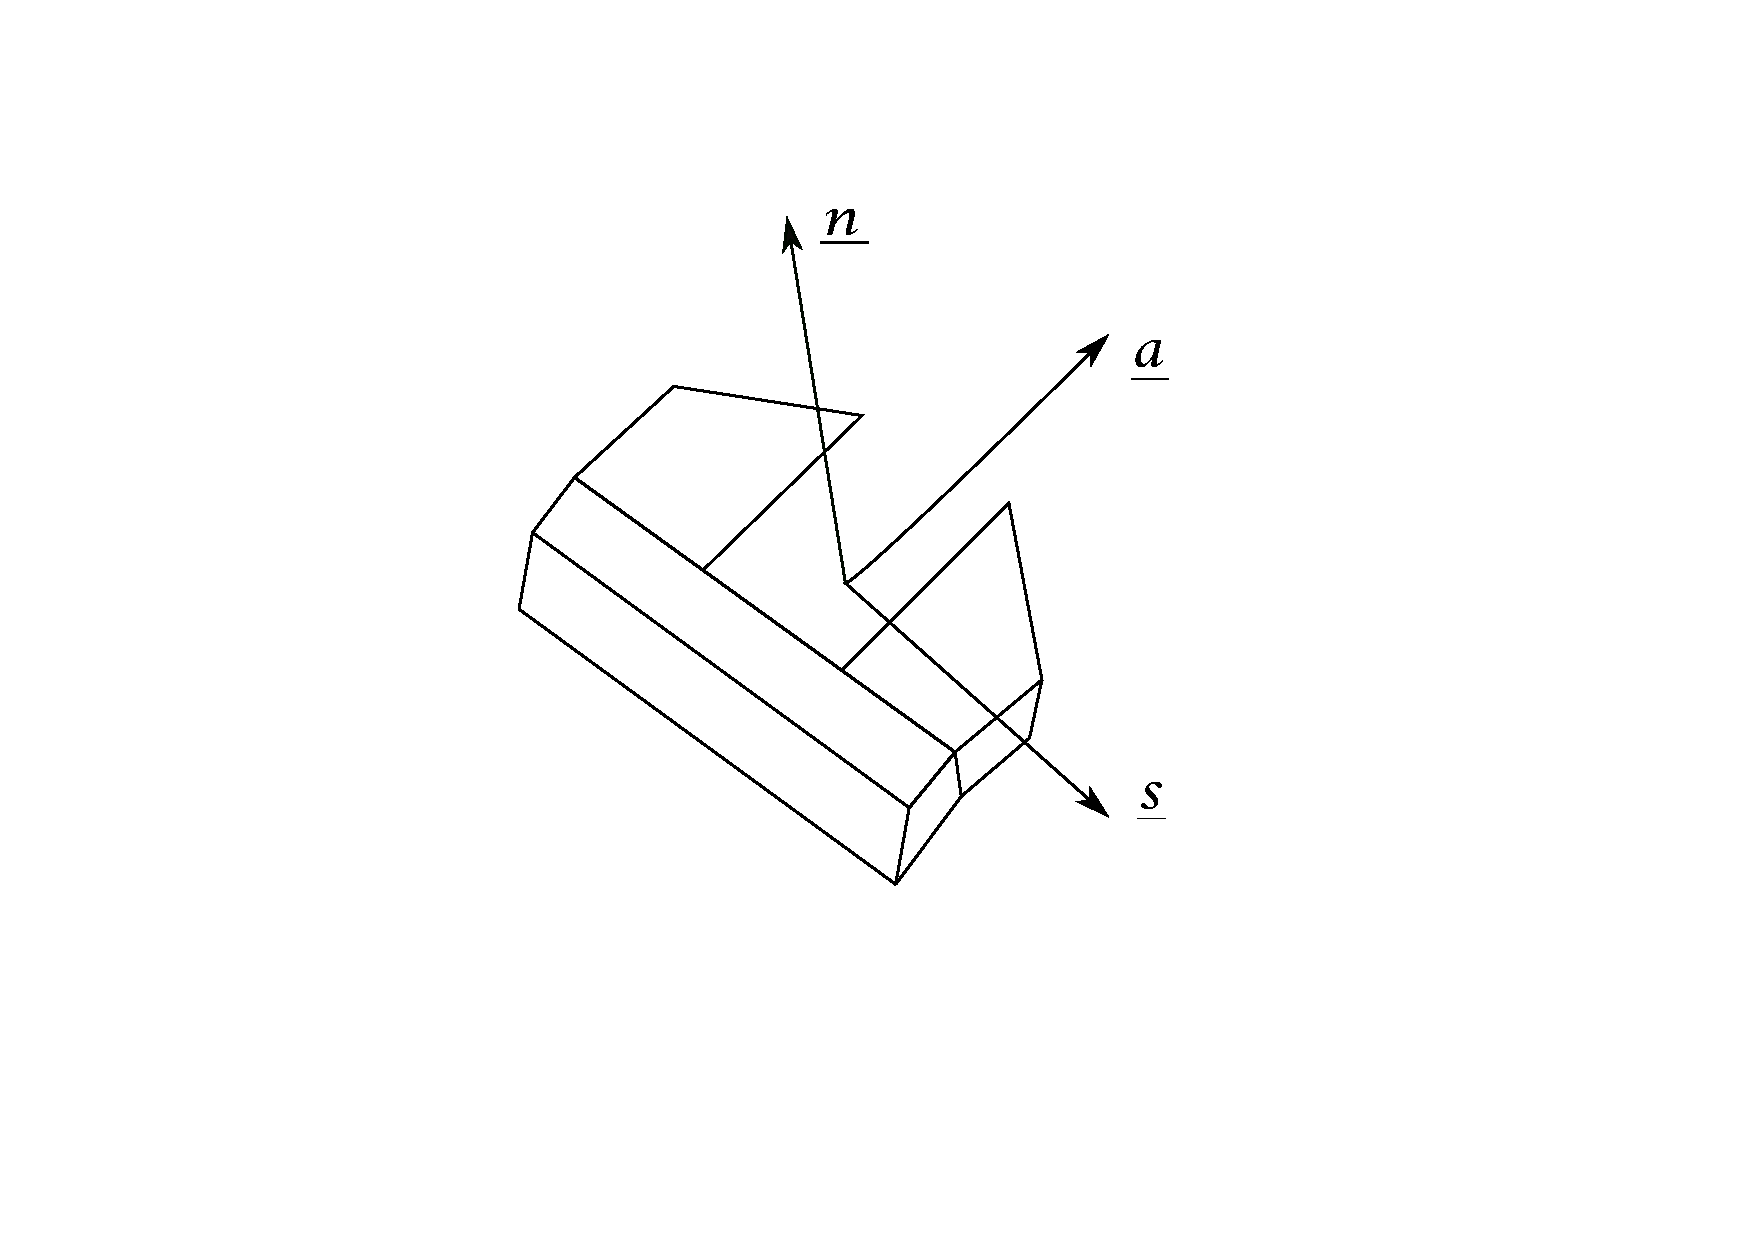
\includegraphics[scale=0.35]{pinzaNSA.pdf}\\
	e consideriamo la matrice:
	\begin{equation*}
		R = 
		\begin{bmatrix}
			n_x & 1 & a_x \\
			0 & s_y & a_y \\
			1 & s_z & a_z
		\end{bmatrix}
	\end{equation*}
	ci chiediamo quanto valgono i termini incogniti. Sfruttando le proprietà di $R$, possiamo dire che $n_x = s_y = s_z = 0$ perchè le colonne devono essere a norma unitaria.\\
	Sappiamo che $\underline{n} \times \underline{s} = \underline{a}$ e sfruttando la \emph{rappresentazione matriciale} del prodotto vettoriale, otteniamo:
	\begin{equation*}
		S(\underline{n})\cdot\underline{s} = 
		\begin{bmatrix}
			0 & -1 & 0 \\
			1 & 0 & 0 \\
			0 & 0 & 0 
		\end{bmatrix}
		\begin{bmatrix}
			1 \\
			0 \\
			0
		\end{bmatrix}
		= 
		\begin{bmatrix}
			0 \\
			1 \\
			0
		\end{bmatrix}
	\end{equation*}
	e otteniamo:
	\begin{equation*}
		R = 
		\begin{bmatrix}
			0 & 1 & 0 \\
			0 & 0 & 1 \\
			1 & 0 & 0 
		\end{bmatrix}
	\end{equation*}
\end{Esercizio}


\newpage
\section{Angoli di Eulero $ZYZ$}
\paragraph{}
Si tratta di una rappresentazione minima che utilizza tre angoli, si fissano due terne: 
\begin{itemize}
	\item terna $\langle0\rangle$ fissa
	\item terna $\langle1\rangle$ mobile rispetto a $\langle0\rangle$
\end{itemize}
Il concetto è che \emph{tre rotazioni successive} in terna corrente formano la \emph{rotazione complessiva}. 
\paragraph{}
Intersecando i piani $x_0y_0$ e $x_1y_1$ si ottiene una retta che chiamiamo \textbf{Linea dei Nodi}. Notiamo che questa linea non è univocamente determinata quando $\underline{k_0} = \pm \underline{k_1}$, ovvero, quando i piani sono paralleli. Inoltre, la linea dei nodi è $\perp$ sia a $z_0$ che a $z_1$.

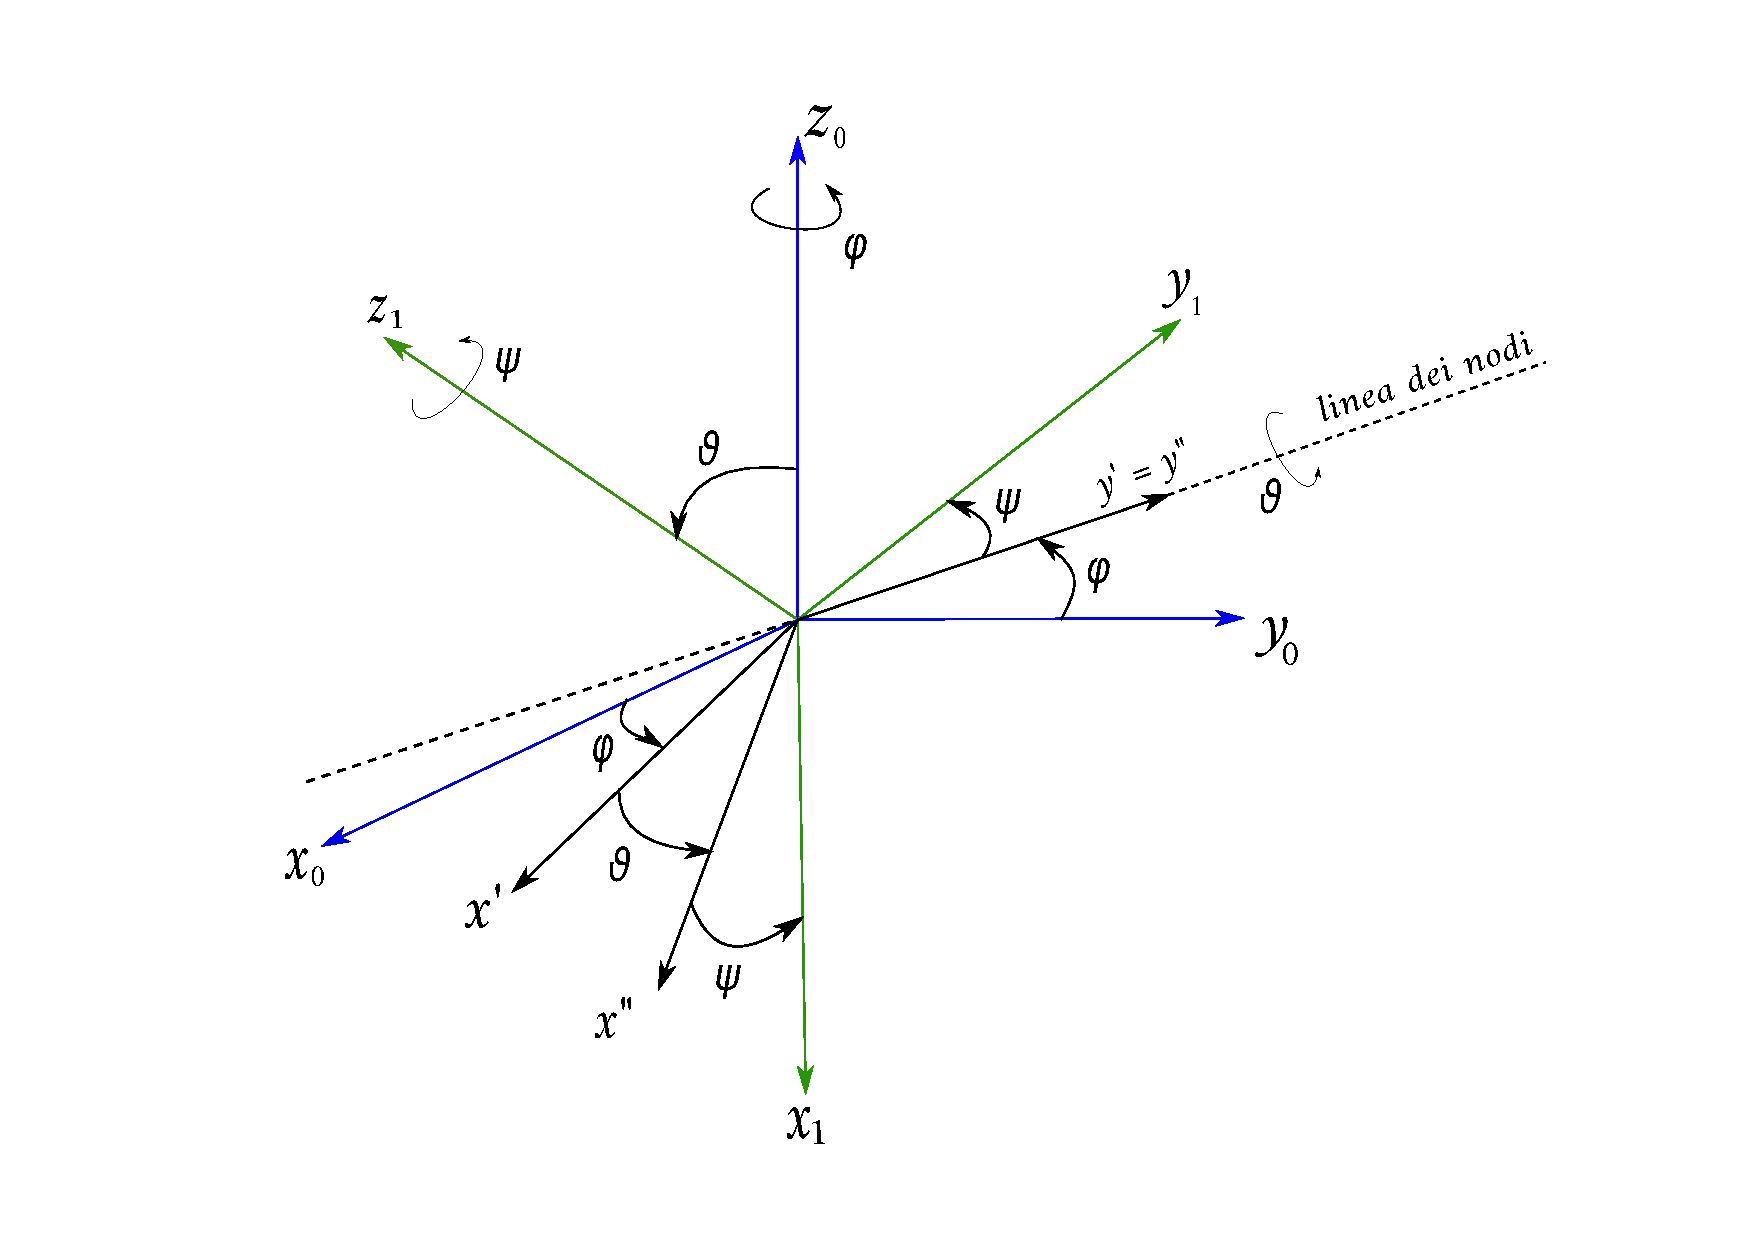
\includegraphics[scale=0.35]{angoliEulero.pdf}
\captionof{figure}{Angoli di Eulero}

\subsubsection{Tre Rotazioni}
\begin{enumerate}
	\item Ruotiamo la terna $\langle0\rangle$ attorno a $z_0$ di un angolo $\varphi$ fino a che $y$ della terna corrente non si allinea con la \emph{linea dei nodi}. Chiamiamo la \emph{terna corrente} $O_{x'y'z'}$ con $z' \equiv z_0$.
	\item Imponiamo, alla terna corrente $O_{x'y'z'}$, una rotazione attorno a $y'$ (\emph{linea dei nodi} $\perp \underline{k_0} \perp \underline{k_1}$ ) di un angolo $\theta$ fino a che l'asse $z$ della \emph{terna corrente} non si allinea con $z_1$. Chiamiamo questa terna $O_{x"y"z"}$ con $y" \equiv y'$ e $z" = z_1$. A questo punto, $z$ è nella sua orientazione, $y" \equiv y'$ è la \emph{linea dei nodi} e $x"y"$ è ruotato di un certo angolo $\psi$ rispetto a $x_1y_1$.
	\item Imponiamo una rotazione $\psi$ attorno a $\underline{k"} \equiv \underline{k_1}$ fino a che $x$ e $y$ della terna corrente non si allineano con $x_1$ e $y_1$.
\end{enumerate}
Otteniamo la composizione in terna corrente seguente:
\begin{equation}
	R_{zyz} = R_z(\varphi)R_{y'}(\theta)R_{z"}(\psi)
\end{equation}

con $z \equiv z_0$, $y' = $\emph{ linea dei nodi} e $z" \equiv z_1$. 

\begin{center}
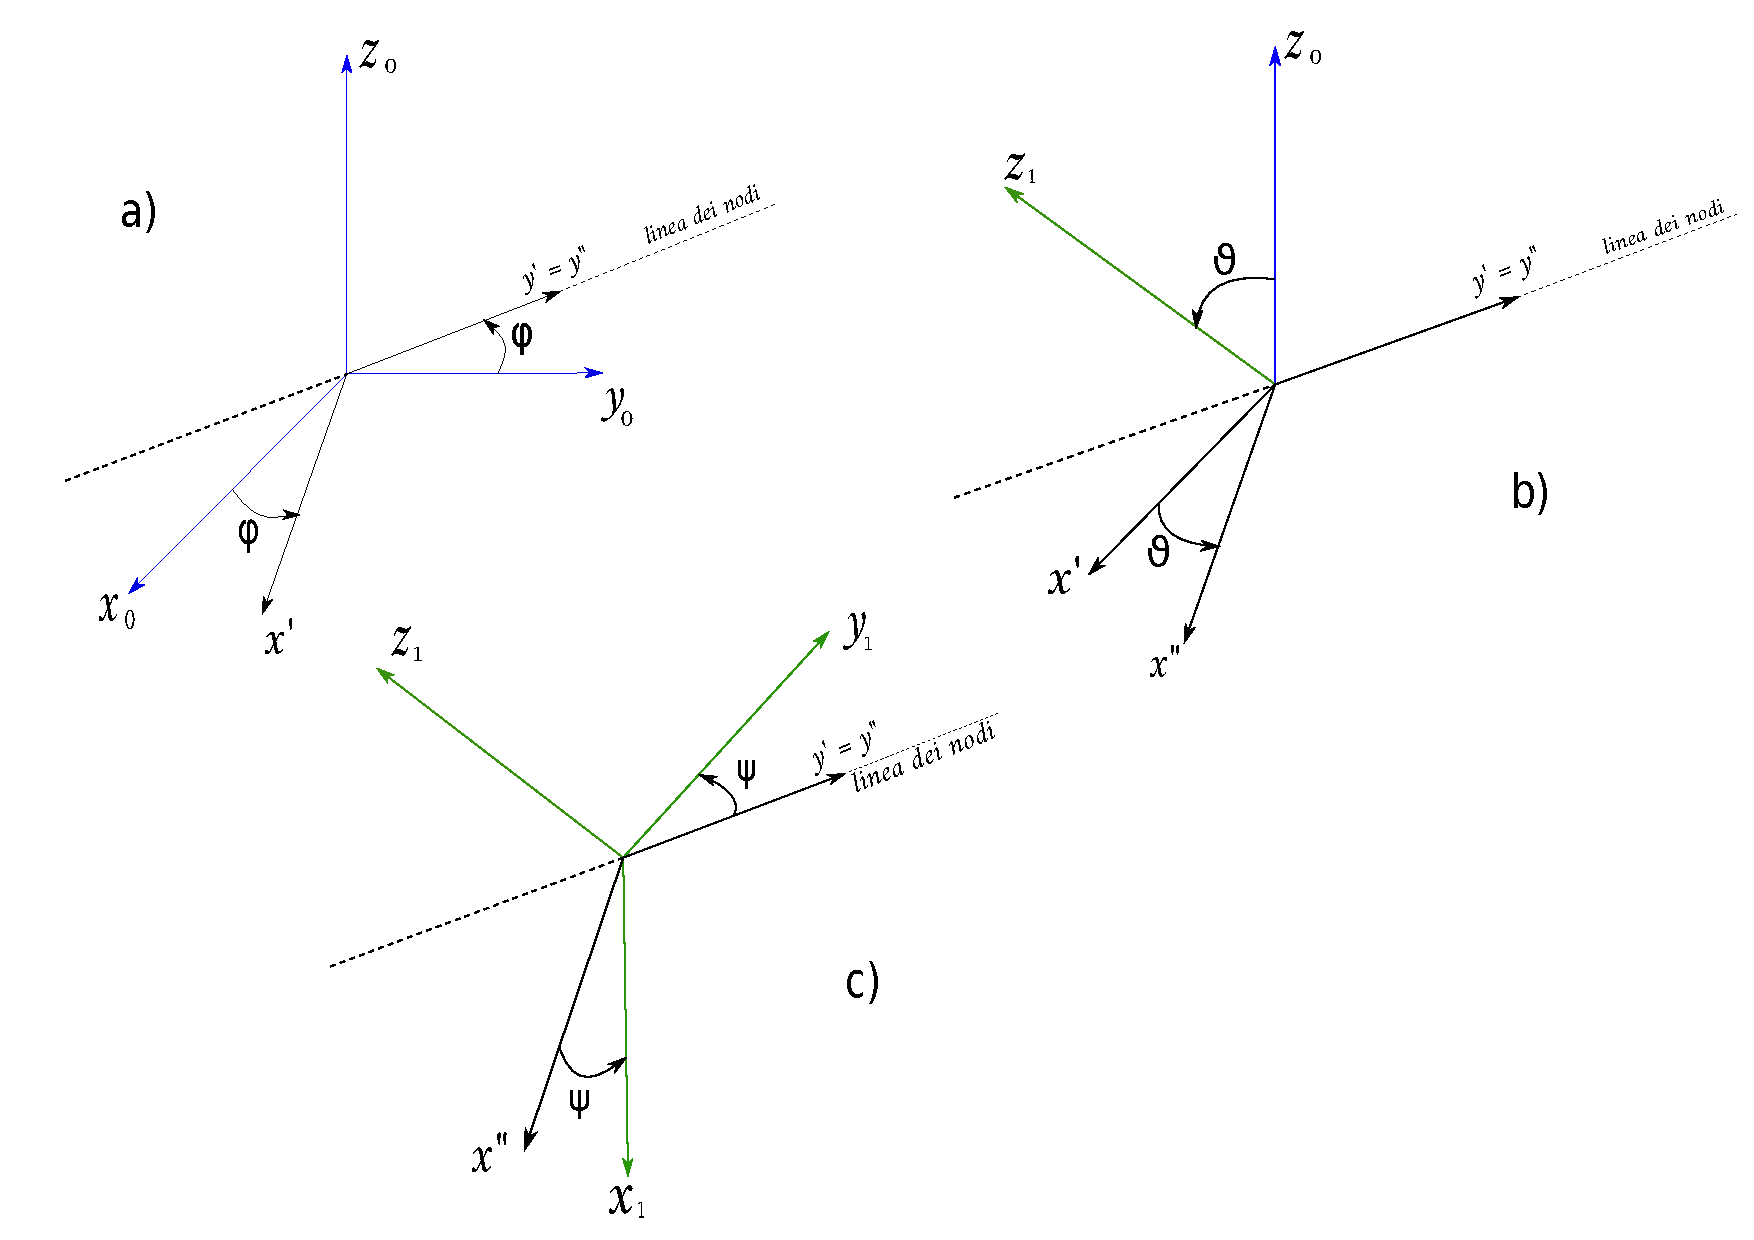
\includegraphics[scale=0.35]{rotazioniEulero.pdf}
\captionof{figure}{Rotazioni di Eulero: a)$R_z(\varphi)$ b)$R_{y'}(\theta)$ c)$R_{z_1}(\psi)$}
\end{center}


\paragraph{}
Scriviamo la matrice complessiva $R_{zyz}$:

\begin{equation*}
	R_{zyz} = R_z(\varphi)R_{y'}(\theta)R_{z"}(\psi) =
	\begin{bmatrix}
		C_{\varphi} & -S_{\varphi} & 0 \\
		S_{\varphi} & C_{\varphi} & 0 \\
		0 & 0 & 1
	\end{bmatrix}
	\cdot
	\begin{bmatrix}
		C_{\theta} & 0 & S_{\theta} \\
		0 & 1 & 0 \\
		-S_{\theta} & 0 & C_{\theta}
	\end{bmatrix}
	\cdot
	\begin{bmatrix}
		C_{\psi} & -S_{\psi} & 0 \\
		S_{\psi} & C_{\psi} & 0 \\
		0 & 0 & 1
	\end{bmatrix}
	=
\end{equation*}
\begin{equation*}
	=
	\begin{bmatrix}
		C_{\varphi}C_{\theta} & -S_{\varphi} & C_{\varphi}S_{\theta} \\
		S_{\varphi}C_{\theta} & C_{\varphi} & S_{\varphi}S_{\theta} \\
		-S_{\theta} & 0 & C_{\theta}
	\end{bmatrix}
	\cdot
	\begin{bmatrix}
		C_{\psi} & -S_{\psi} & 0 \\
		S_{\psi} & C_{\psi} & 0 \\
		0 & 0 & 1
	\end{bmatrix}
	=
\end{equation*}
\begin{equation*}
	=
	\begin{bmatrix}
		C_{\varphi}C_{\theta}C_{\psi} - S_{\varphi}S_{\psi} & -C_{\varphi}C_{\theta}C_{\psi} - S_{\varphi}S_{\psi} & C_{\varphi}S_{\theta} \\
		S_{\varphi}C_{\theta}C_{\psi} - C_{\varphi}S_{\psi} & -S_{\varphi}C_{\theta}C_{\psi} - C_{\varphi}C_{\psi} & S_{\varphi}S_{\theta} \\
		-S_{\theta}C_{\psi} & S_{\theta}S_{\psi} & C_{\theta}
	\end{bmatrix}
\end{equation*}

\subsubsection{Discorso inverso}
Spesso si ha il problema inverso, ovvero, data una $R$ qualsiasi, calcolare $\varphi$, $\theta$ e $\psi$. Osserviamo: 
\begin{itemize}
	\item gli elementi $r_{13}$ e $r_{23}$ sono pari rispettivamente a $C_{\varphi}$, $S_{\varphi}$ moltiplicati per $S_{\theta} = \sin(\theta)$.
	\item gli elementi $r_{31}$ e $r_{32}$ sono pari rispettivamente a $C_{\psi}$, $S_{\psi}$ moltiplicati per $S_{\theta} = \sin(\theta)$. 
\end{itemize}
\newpage
Otteniamo tre rami di soluzione:
\begin{itemize}
	\item $\sin{\theta} > 0$:
	\begin{itemize}
		\item[$\rightarrow$] $\varphi = atan_2(r_{23}, r_{13})$
		\item[$\rightarrow$] $\psi = atan_2(r_{32}, -r_{31})$
		\item[$\rightarrow$] $\theta = atan_2(\sqrt{r_{13}^2 + r_{23}^2}, r_{33})$ perché $r_{13}^2 + r_{23}^2 = (C_{\varphi}^2 + S_{\varphi}^2)S_{\theta}^2 = S_{\theta}^2$
	\end{itemize}
	\item $\sin{\theta} < 0$:
	\begin{itemize}
		\item[$\rightarrow$] $\varphi = atan_2(-r_{23}, -r_{13})$
		\item[$\rightarrow$] $\psi = atan_2(-r_{32}, r_{31})$
		\item[$\rightarrow$] $\theta = atan_2(-\sqrt{r_{13}^2 + r_{23}^2}, r_{33})$
	\end{itemize}
	\item $\sin{\theta} = 0$: In questo caso distinguiamo due ulteriori casi, ovvero, $\theta = 0$ e $\theta = \pm \pi$. Possiamo discriminare questi due casi \emph{osservando preliminarmente} $r_{33}$.
	\begin{itemize}
		\item[•] $r_{33}= 1 (\Rightarrow \theta = 0)$: otteniamo la matrice\\ $R_{zyz}(\theta)|_{\theta = 0} = 
		\begin{bmatrix}
			C_{\varphi\psi} & -S_{\varphi\psi} & 0 \\
			S_{\varphi\psi} & C_{\varphi\psi} & 0 \\
			0 & 0 & 1
		\end{bmatrix} \quad$ con $C_{\varphi\psi} = \cos(\varphi + \psi)$\\ Quindi con $\theta = 0$ possiamo determinare $\varphi + \psi = atan_2(r_{21}, r_{11})$, ma calcolare $\varphi$ e $\psi$ non ha molto senso, dunque si ha una \emph{singolarità di rappresentazione}.
		\item[•] $r_{33}= -1 (\Rightarrow \theta = \pm \pi)$: otteniamo la matrice\\ 
	\begin{center}
$R_{zyz}(\theta)|_{C_{\theta} = -1} = 
		\begin{bmatrix}
			-(C_{\varphi}C_{\psi} + S_{\varphi}S_{\psi}) & -S_{\varphi}C_{\psi} + C_{\varphi}S_{\psi} & 0 \\
			-S_{\varphi}C_{\psi} + C_{\varphi}S_{\psi} & C_{\varphi}C_{\psi} + S_{\varphi}S_{\psi} & 0 \\
			0 & 0 & -1
		\end{bmatrix}$
		= \\
		$=\begin{bmatrix}
			-\cos(\varphi-\psi) & -\sin(\varphi-\psi) & 0\\
			-\sin(\varphi-\psi) & \cos(\varphi-\psi) & 0 \\
			0 & 0 & -1
		\end{bmatrix}$\\
	\end{center}
Anche in questo caso non possiamo determinare $\varphi$ e $\psi$ ma solo la loro differenza. Si nota che $\underline{k_0} = -\underline{k_1}$.
	\end{itemize}
\end{itemize}
\chapter{Il metodo di Denavit-Hartenberg}
Il metodo di \emph{Denavit-Hartemberg}, brevemente indicato con \emph{D-H}, è il più diffuso per la descrizione cinematica di meccanismi a catena aperta semplice (robot seriali). Il metodo può comunque essere utilizzato anche per meccanismi a catena chiusa ma non tratteremo questa sua possibile applicazione.

\paragraph{}
Dato un meccanismo seriale, il metodo permette di fissare in modo sistematico delle terne di riferimento su ognuno dei membri che compongono il meccanismo (dal telaio fino all’organo terminale che sia  pinza, mano o utensile) e di ricavare le leggi di trasformazione di coordinate che legano tra loro due terne contigue.

\section{Rototraslazioni}
In generale, due terne $\langle0\rangle$, $\langle1\rangle$ hanno diversa orientazione e origine non coincidente.\\
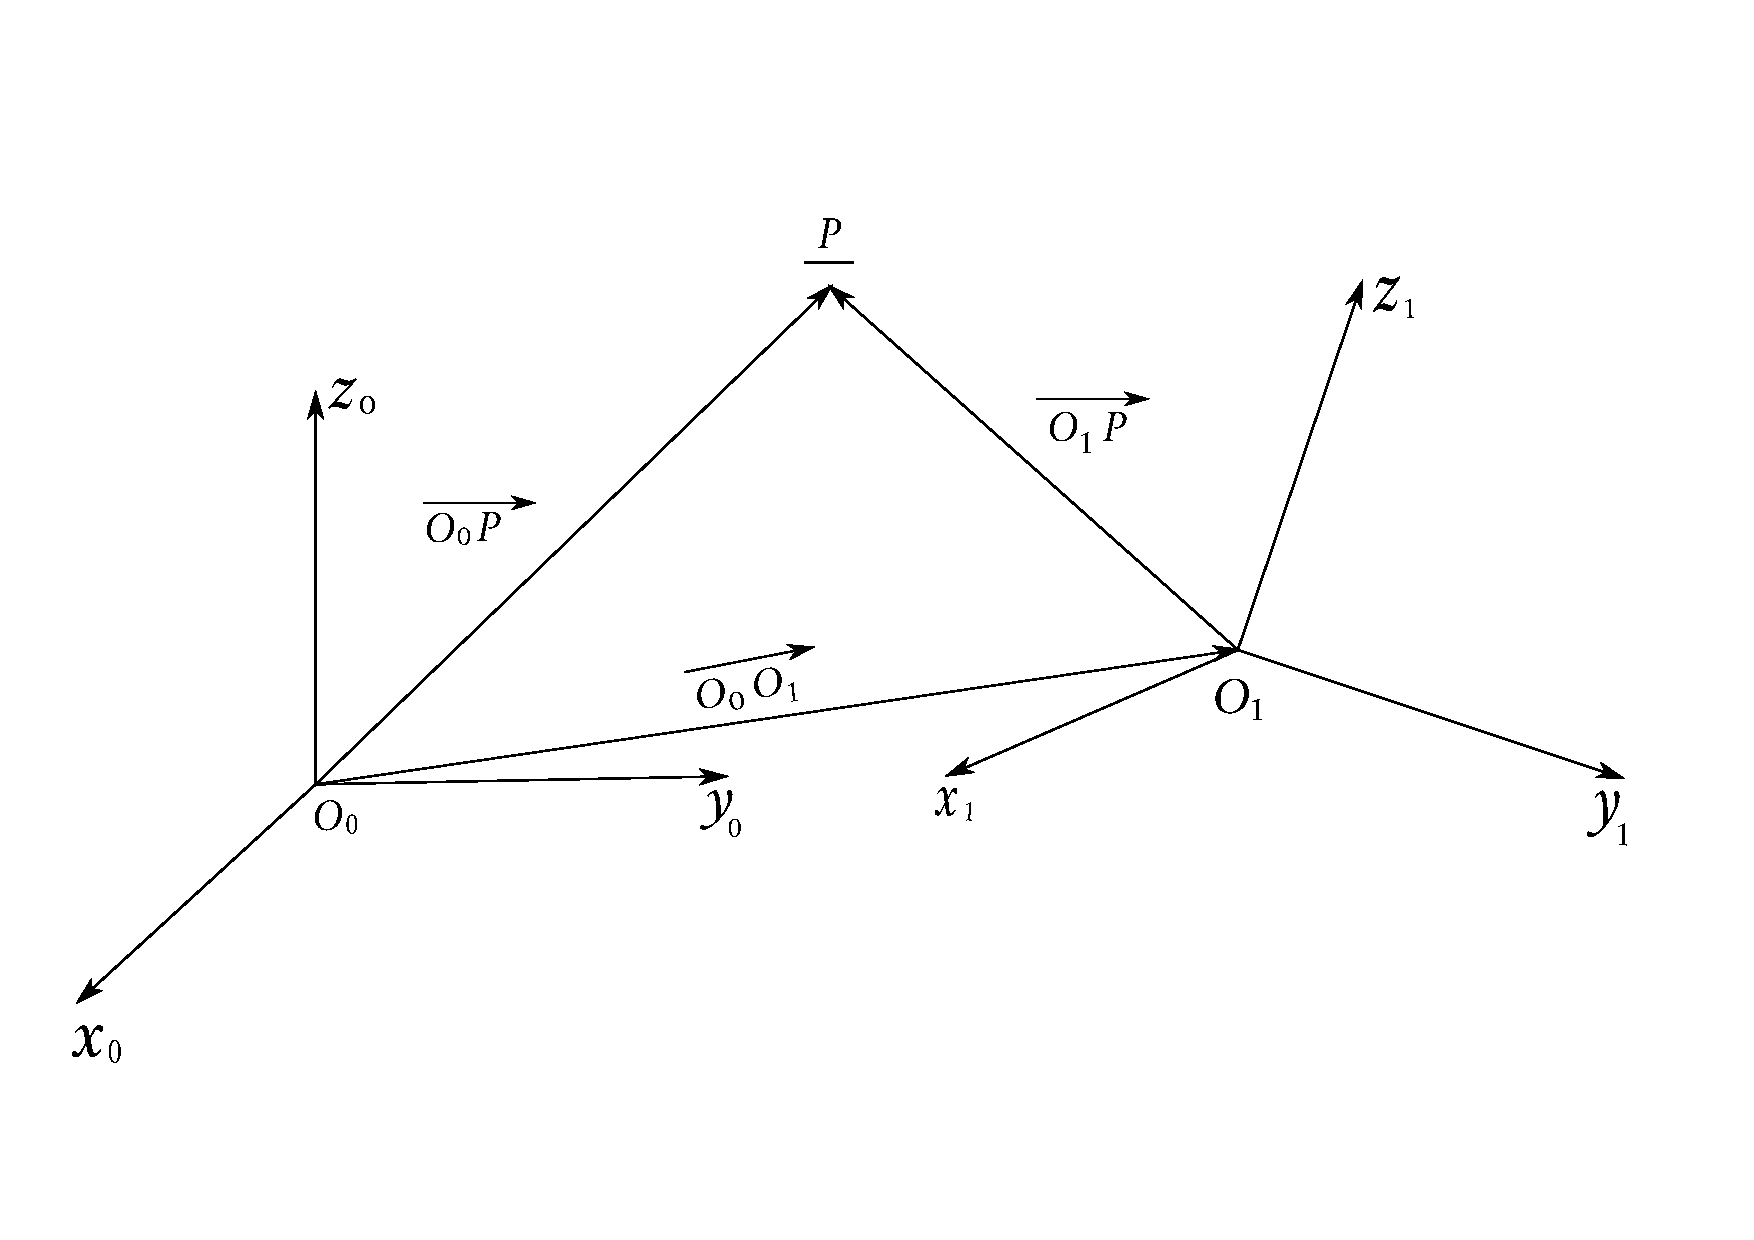
\includegraphics[scale=0.35]{rototraslazione.pdf}

Otteniamo, $\vec{O_{0}P} = \vec{O_0O_1} + \vec{O_1P}$, e scriviamo questa espressione in $\mathbb{R}^3$ con tutti i vettori riferiti alla terna $\langle0\rangle$: 
\begin{equation} \label{somma}
	^0\underline{P} = \,^0\underline{O_1} + R_1^0 \; ^1\underline{P} 
\end{equation}
L'operazione \eqref{somma} presenta una somma e una moltiplicazione, ma usande le \emph{coordinate omogenee}, l'equazione diventa una sola moltiplicazione.

\section{Coordinate Omogenee}
Per identificare un punto $\underline{P}$ nel piano si usano tre numeri $\underline{P}=
\begin{bmatrix}
	P_x & P_y & P_z
\end{bmatrix}^T$ 
e l'informazione contenuta in questi tre numeri può essere osservata anche se li moltiplichiamo per una costante arbitraria $\lambda \neq 0$ purchè si memorizzi la costante stessa. Pertanto il punto $\underline{P}$ possiamo rappresentarlo con quattro numeri nello spazio contenenti la stessa informazione della rappresentazione nel piano. Otteniamo:
\begin{equation}
	\underline{\tilde{P}} = 
	\begin{bmatrix}
		\lambda\underline{P} \\
		\lambda
	\end{bmatrix}
	=
	\begin{bmatrix}
		\lambda P_x \\
		\lambda P_y \\
		\lambda P_z \\
		\lambda
	\end{bmatrix}
\end{equation}
con $\underline{\tilde{P}}$ contenente la stessa informazione di $\underline{P}$. Nel seguito useremo sempre $\lambda = 1$.

\subsection{Trasformazioni omogenee}
Vediamo il \emph{cambio di coordinate} tra $\langle0\rangle$ e $\langle1\rangle$, con origine distinta, in \emph{coordinate omogenee}:
\begin{equation}
	\begin{cases}
		^0\underline{P} = R_1^0 \, ^1\underline{P} + \,^0\underline{O_1} = 			\begin{bmatrix}
			R_1^0 & ^0\underline{O_1}
		\end{bmatrix}
		\cdot
		\begin{bmatrix}
			^1\underline{P} \\
			1
		\end{bmatrix}\\
		1 = 
		\begin{bmatrix}
			0 & 0 & 0 & 1
		\end{bmatrix}
		\cdot
		\begin{bmatrix}
			^1\underline{P} \\
			1
		\end{bmatrix}
	\end{cases}
\end{equation}

ottenendo:
\begin{equation}
	\begin{bmatrix}
		^0\underline{P} \\
		1
	\end{bmatrix}
	=
	\begin{bmatrix}
		R_1^0 & ^0\underline{O_1} \\
		0\,0\,0 & 1
	\end{bmatrix}
	\begin{bmatrix}
		^1\underline{P} \\
		1
	\end{bmatrix}
	\Rightarrow
	\underline{^0\tilde{P}} = T_1^0 \; \underline{^1\tilde{P}}
\end{equation}

con:
\begin{equation} \label{trasformazione_omogenea}
	T_1^0 =
	\begin{bmatrix}
		R_1^0 & ^0\underline{O_1} \\
		0\,0\,0 & 1
	\end{bmatrix}
\end{equation}
$T_1^0$ della \eqref{trasformazione_omogenea} si dice \emph{matrice di trasformazione omogenea}, infatti, opera la trasformazione di coordinate omogenee di un punto tra due terne.
\subsection{Composizione di rototraslazioni successive}
Supponiamo di avere tre terne $\langle0\rangle$, $\langle1\rangle$, $\langle2\rangle$. Sia $T_1^0$ la matrice di trasformazione dalla terna $\langle0\rangle$ alla terna $\langle1\rangle$ e $T_2^1$ la matrice di trasformazione dalla terna $\langle1\rangle$ alla terna $\langle2\rangle$. Ci poniamo l'obiettivo di calcolare $T_2^0$. Per il generico punto $\underline{P}$, opportunamente riferito in coordinate omogenee rispetto alle tre terne, varranno le seguenti equazioni:
\begin{align} \label{p0} 
	^0\underline{\tilde{P}} = T_1^0 \, ^1\underline{\tilde{P}} \\
	\label{p1}
	^1\underline{\tilde{P}} = T_2^1 \, ^2\underline{\tilde{P}} \\
	^0\underline{\tilde{P}} = T_2^0 \, ^2\underline{\tilde{P}}
\end{align} 
Sostituendo l'espressione $^1\underline{\tilde{P}}$ della \eqref{p1} nella \eqref{p0}, otteniamo:
\begin{equation}
	^0\underline{\tilde{P}} =  T_1^0 \, T_2^1 \, ^2\underline{\tilde{P}}
\end{equation}
dovendo valere la (2.8) e la (2.9) per \emph{qualsiasi punto} $\underline{P}$, otterremo per $T_2^0$ la seguente espressione:
\begin{equation}
	T_2^0 = T_1^0 \; T_2^1
\end{equation}
\paragraph{}
Si generalizza a $n+1$ terne, ognuna mappata rispetto alla precedente da $T_{i}^{i-1}$, otteniamo:

\begin{equation}
	T_n^0 = T_1^0 \; T_2^1 \; \cdots \; T_{n-1}^{n-2} \; T_n^{n-1}
\end{equation}

\subsubsection{Calcolo rapido di $T_0^1$}
La matrice $T_0^1 = (T_1^0)^{-1}$ si può calcolare facendo l'inversa della \eqref{trasformazione_omogenea}, ma esiste un'altra strada più rapida, consideriamo $^0\underline{P} = R_1^0 \, ^1\underline{P} + \,^0\underline{O_1}$ e calcoliamo $^1\underline{P}$ da questa equazione:

\begin{equation*}
	^0\underline{P} = R_1^0 \; ^1\underline{P} + \,^0\underline{O_1} \Rightarrow R_1^0 \; ^1\underline{P} = \,^0\underline{P} - ^0\underline{O_1} \Rightarrow \,^1\underline{P} = (R_1^0)^T (^0\underline{P} - ^0\underline{O_1})
\end{equation*}
ottenendo:
\begin{equation*}
	\,^1\underline{P} = R_0^1 \; ^0\underline{P} - R_0^1 \; ^0\underline{O_1}
\end{equation*}
e pertanto otteniamo:
\begin{equation}
	T_0^1 =
	\begin{bmatrix}
		R_0^1 & -R_0^1 \; ^0\underline{O_1} \\
		0\,0\,0 & 1
	\end{bmatrix}
\end{equation}
\newpage
\section{Metodo di Denavit-Hartenberg}
Si tratta di un \emph{metodo sistematico} per descrivere catene cinematiche, ovvero, insiemi di corpi rigidi collegati tra loro da \emph{coppie cinematiche} rotoidali o prismatiche. Da qui in avanti le coppie cinematiche le chiameremo \emph{giunti}.

\subsection{Passi del metodo per grandi linee}
\begin{enumerate}
	\item Si numerano i membri (link), da $0$ a $n$.
	\item Si numerano i giunti, da $1$ a $n$.
	\item Si fissano, con alcune regole, $n+1$ terne ai vari link.
	\item Si calcola $T_i^{i-1}\quad\forall n$.
	\item Si ottiene $T_0^n = T_0^1\,T_2^1\,\cdots\,T_{n-1}^{n-2}\,T_n^{n-1}$
\end{enumerate}

Il metodo \emph{D-H} ci permette di ridurre da sei a quattro il numero di parametri necessari per costruire $T_i^{i-1}$, infatti, tre parametri saranno fissi ed uno sarà variabile (\emph{coordinata di giunto}).

\subsection{Regole generali per fissare la terna $i$ sul link $i$}
\begin{enumerate}
	\item[0.] Una volta numerati link e giunti
	\item[1.] L'asse $z_{i-1}$ si sceglie:
	\begin{itemize}
		\item Coincidente con l'asse di rotazione del giunto $i$ se questo è rotoidale, scegliendo il verso con buonsenso.
		\item Parallelo alla direzione di moto del giunto $i$ se questo è prismatico.
	\end{itemize}
	notiamo che l'asse $z_n$ è arbitrario e quindi lo possiamo scegliere con "buonsenso".
	\item[2.]In generale si sceglie l'asse $x_i$ come la retta di minima distanza, orientata da $z_{i-1}$ a $z_i$. Questa regola ha dei casi particolari:
	\begin{itemize}
		\item Se non esiste l'asse $z_{i-1}$ allora non posso applicare la regola per fissare $x_0$, quindi fisso questo asse arbitrariamente con il vincolo $x_{0}\,\perp\,z_{0}$ così scegliamo anche $O_0$.
		\item Se $z_{i-1}\parallel z_i$ allora $x_i$ va scelto arbitrariamente pur facendo presente che il verso da $z_{i-1}$ a $z_i$ è definito.
		\item Se $z_{i-1}$ e $z_i$ sono \emph{incidenti} allora la retta di minima distanza degenera nella normale comune ed il verso di $x_i$ va scelto arbitrariamente tale che $\underline{i_i} = \pm \underline{k_{i-1}} \times \underline{k_i}$ e poniamo quindi il vincolo di ortogonalità dell'asse $x_i$ sia per $z_i$ che per $z_{i-1}$.
	\end{itemize}
\end{enumerate}

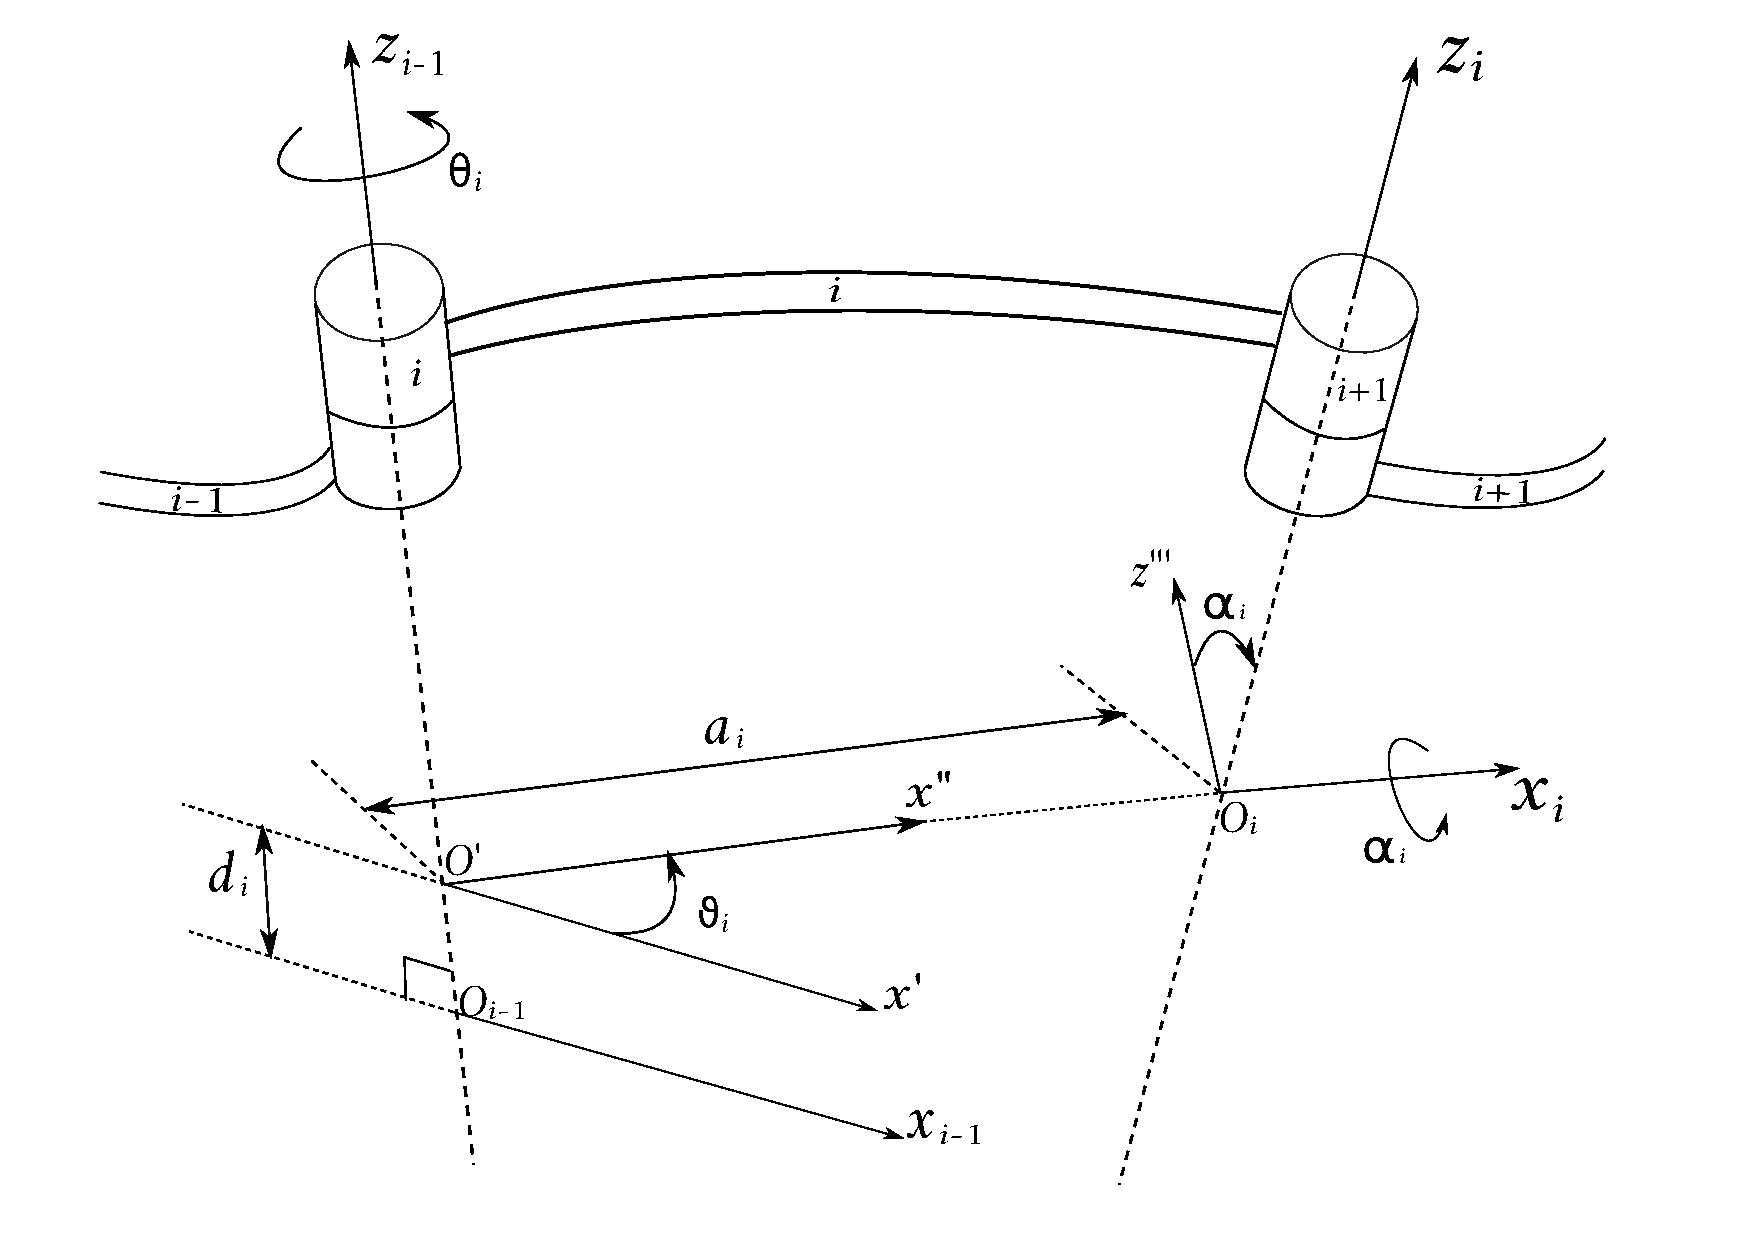
\includegraphics[scale=0.4]{metodoDH.pdf}
\captionof{figure}{Terne e trasformazioni nel metodo D-H}

\subsection{Calcolo di $T_i^{i-1}$}
Per ottenere $T_i^{i-1}$ scomponiamola in quattro trasformazioni successive specificate in terna corrente che portino $\langle i-1 \rangle$ a sovrapporsi alla terna $\langle i \rangle$:
\begin{enumerate}
	\item Trasformazione lungo $z_{i-1}$ di una quantità $d_{i}\gtreqless0$, fino a che l'origine della terna corrente non si sposta in $O'\,\in\,x_i$.
	\item Rotazione attorno a $z_{i-1}$ di un angolo $\theta_{i}\lesseqgtr0$, fino a che l'asse $x$ della terna corrente non si allinea con $x_i$.
	\item Traslazione lungo $x_i$ di una quantità $a_{i}\geqslant0$ (lunghezza del segmento di minima distanza tra $z_{i-1}$ e $z_i$), fino a che l'origine non va a coincidere con $O_i$.
	\item Rotazione attorno a $x_i$ di un angolo $\alpha_{i}\lesseqgtr0$, fino a che la terna corrente non è allineata con la terna $<i>$.
\end{enumerate}
Notiamo che $\alpha_i$ e $a_i$ sono sempre fissi, $d_i$ è variabile se il giunto $i$ è prismatico e $\theta_i$ è variabile se il giunto $i$ è rotoidale.

\paragraph{}
Vediamo le quattro trasformazioni:
\begin{equation*}
	1) =
	\begin{bmatrix}
		1 & 0 & 0 & 0 \\
		0 & 1 & 0 & 0 \\
		0 & 0 & 1 & d_i \\
		0 & 0 & 0 & 1
	\end{bmatrix}
	\quad 2) =
	\begin{bmatrix}
		C_{\theta_i} & -S_{\theta_i} & 0 & 0 \\
		S_{\theta_i} & C_{\theta_i} & 0 & 0 \\
		0 & 0 & 1 & 0 \\
		0 & 0 & 0 & 1
	\end{bmatrix}
\end{equation*}
\begin{equation*}
	3) =
	\begin{bmatrix}
		1 & 0 & 0 & a_i \\
		0 & 1 & 0 & 0 \\
		0 & 0 & 1 & 0 \\
		0 & 0 & 0 & 1
	\end{bmatrix}
	\quad 4) =
	\begin{bmatrix}
		1 & 0 & 0 & 0 \\
		0 & C_{\alpha_i} & -S_{\alpha_i} & 0 \\
		0 & S_{\alpha_i} & C_{\alpha_i} & 0 \\
		0 & 0 & 0 & 1
	\end{bmatrix}
\end{equation*}
a questo punto facendo il prodotto otteniamo,
\begin{equation*}
	1)\cdot2) =
	\begin{bmatrix}
		C_{\theta_i} & -S_{\theta_i} & 0 & 0 \\
		S_{\theta_i} & C_{\theta_i} & 0 & 0 \\
		0 & 0 & 1 & d_i \\
		0 & 0 & 0 & 1
	\end{bmatrix}
	\quad 3)\cdot4) =
	\begin{bmatrix}
		1 & 0 & 0 & a_i \\
		0 & C_{\alpha_i} & -S_{\alpha_i} & 0 \\
		0 & S_{\alpha_i} & C_{\alpha_i} & 0 \\
		0 & 0 & 0 & 1
	\end{bmatrix}
\end{equation*}
e facendo il prodotto tra queste due matrici otteniamo la \emph{matrice di trasformazione complessiva} $T_i^{i-1}$:
\begin{equation}
	T_i^{i-1} = 
	\begin{bmatrix}
		C_{\theta_i} & -C_{\alpha_i}\,S_{\theta_i} & S_{\alpha_i}\,S_{\theta_i} & a_i\,C_{\theta_i} \\
		S_{\theta_i} & C_{\alpha_i}\,C_{\theta_i} & -S_{\alpha_i}\,C_{\theta_i} & a_i\,S_{\theta_i} \\
		0 & S_{\alpha_i} & C_{\alpha_i} & d_i \\
		0 & 0 & 0 & 1
	\end{bmatrix}
\end{equation}

\subsubsection{Esercizio:}
Consideriamo un manipolatore planare $3R$ (tre giunti rotoidali) e applichiamo il metodo $D-H$.

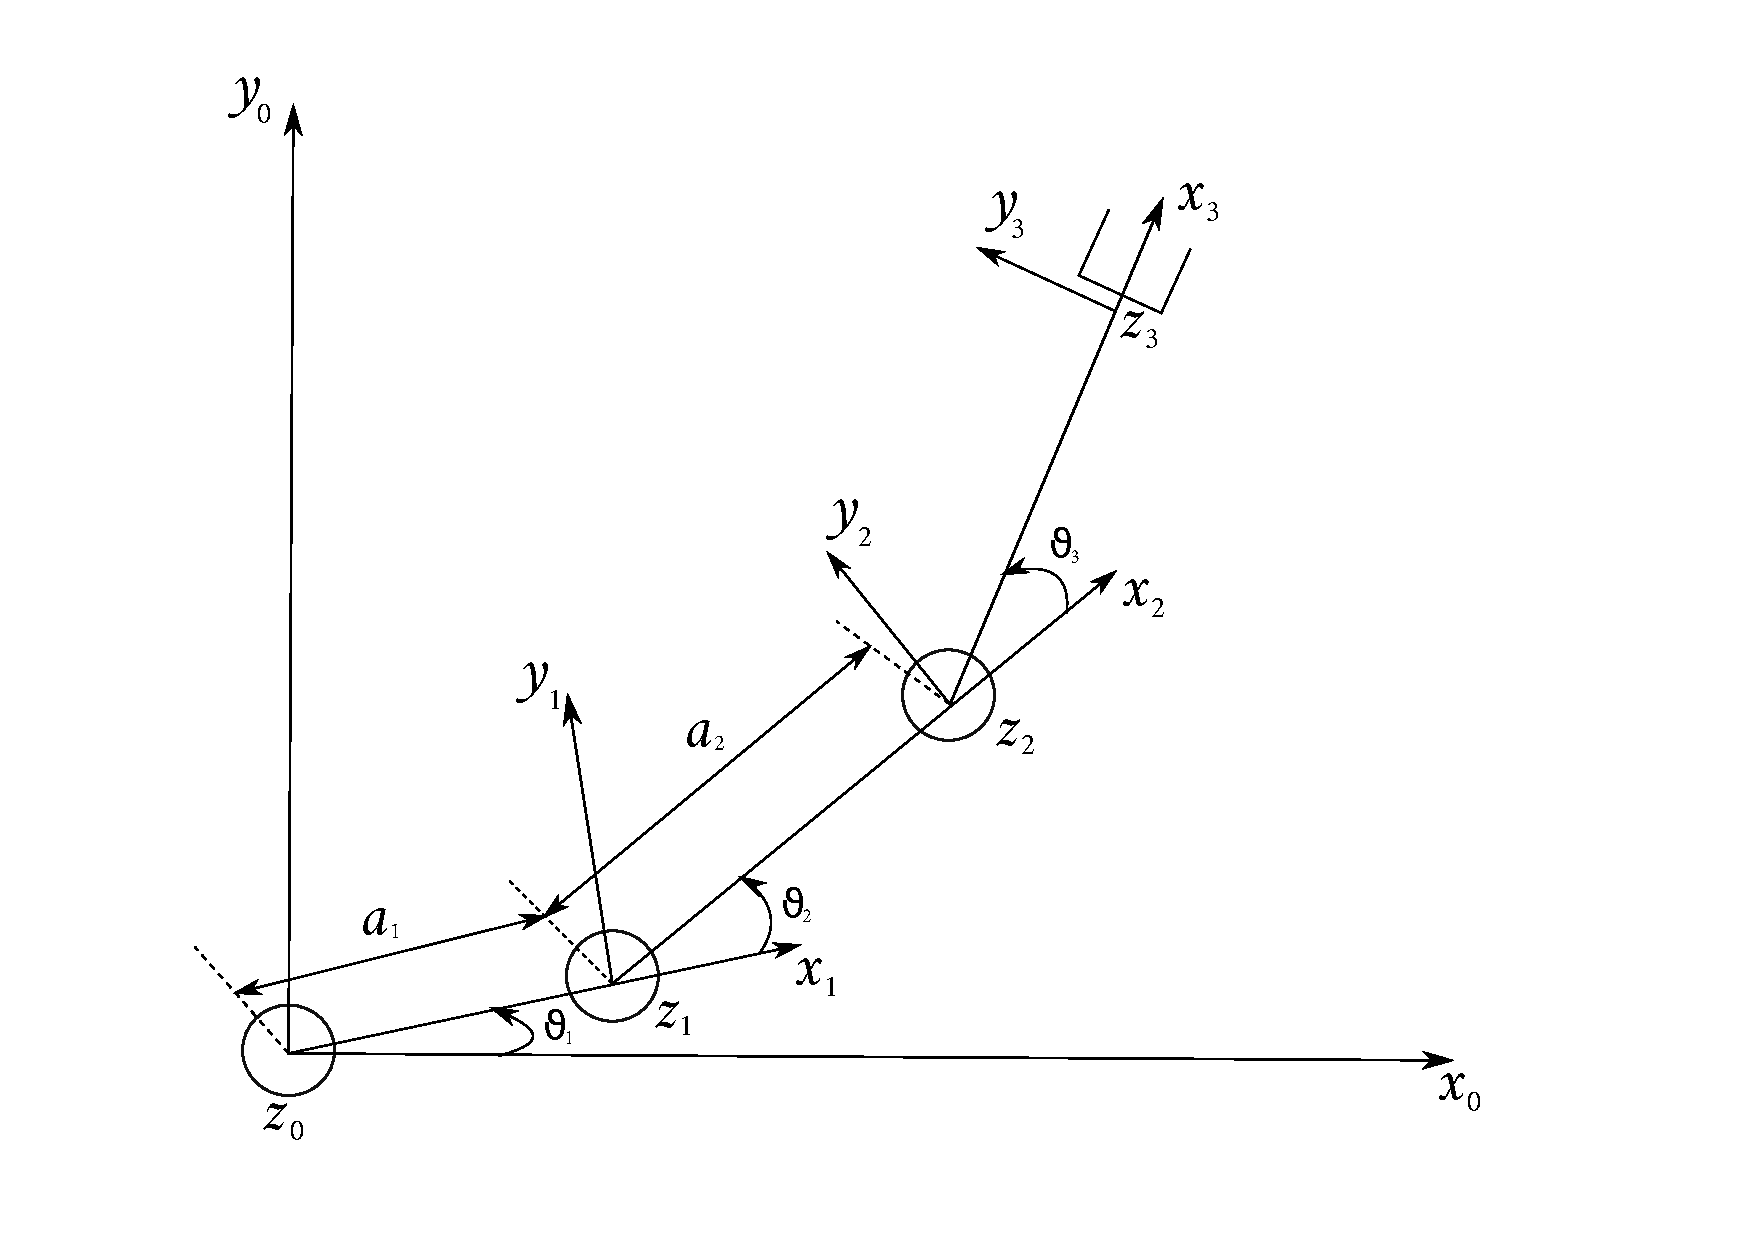
\includegraphics[scale=0.4]{manipolatore3R.pdf}
\captionof{figure}{Manipolatore planare a 3 gradi di libertà, schema cinematico}

Scriviamo la tabella $D-H$:\\
\begin{center}
$
\begin{array}{ccccc}
\toprule
Giunti & d_1 & \theta_i & a_i & \alpha_i \\
\midrule
1 & 0 & q_1 & l_1 & 0 \\
2 & 0 & q_2 & l_2 & 0 \\
3 & 0 & q_3 & l_3 & 0 \\
\bottomrule
\end{array}
$
\end{center}

\paragraph{}
Abbiamo tre modi di procedere:
\begin{itemize}
	\item Metodo sistematico: dalla tabella calcolo $T_1^0$, $T_2^1$, $T_3^2$ e poi le moltiplico.
	\item Metodo intermedio: scrivo "a occhio" le tre matrici e le moltiplico.
	\item Metodo geometrico: in questo caso ho meno calcoli.
\end{itemize}

Otteniamo:
\begin{equation}
	T_3^0 = 
	\begin{bmatrix}
		C_{123} & -S_{123} & 0 & a_1\,C_{\theta_i}+a_2\,C_{12}+ a_3\,C_{123} \\
		S_{123} & C_{123} & 0 & a_1\,S_{\theta_i}+a_2\,S_{12}+ a_3\,S_{123} \\
		0 & 0 & 1 & 0 \\
		0 & 0 & 0 & 1 \\
	\end{bmatrix}
\end{equation}
con: $C_{12} = \cos(\theta_1 + \theta_2)$ e $C_{123} = \cos(\theta_1 + \theta_2 + \theta_3)$.

\section{Manipolatore Antropomorfo}
Applichiamo il metodo \emph{D-H} ad un robot a tre gradi di libertà (\emph{DOF, Degree of Freedom}). Questo manipolatore prende il nome di \emph{antropomorfo} perchè ricorda un braccio umano. I membri sono numerati da $0$ a $3$. Sono presenti tre giunti rotoidali numerati da $1$ a $3$ con le seguenti proprietà:
\begin{itemize}
	\item $Giunto\, 1$: ha asse verticale.
	\item $Giunto\, 2 \,(spalla)$: ha asse orizzontale ed è ortogonale al giunto 1.
	\item $Giunto\, 3 \, (gomito)$: ha asse orizzontale ed è parallelo al giunto 2.
\end{itemize}

\begin{center}
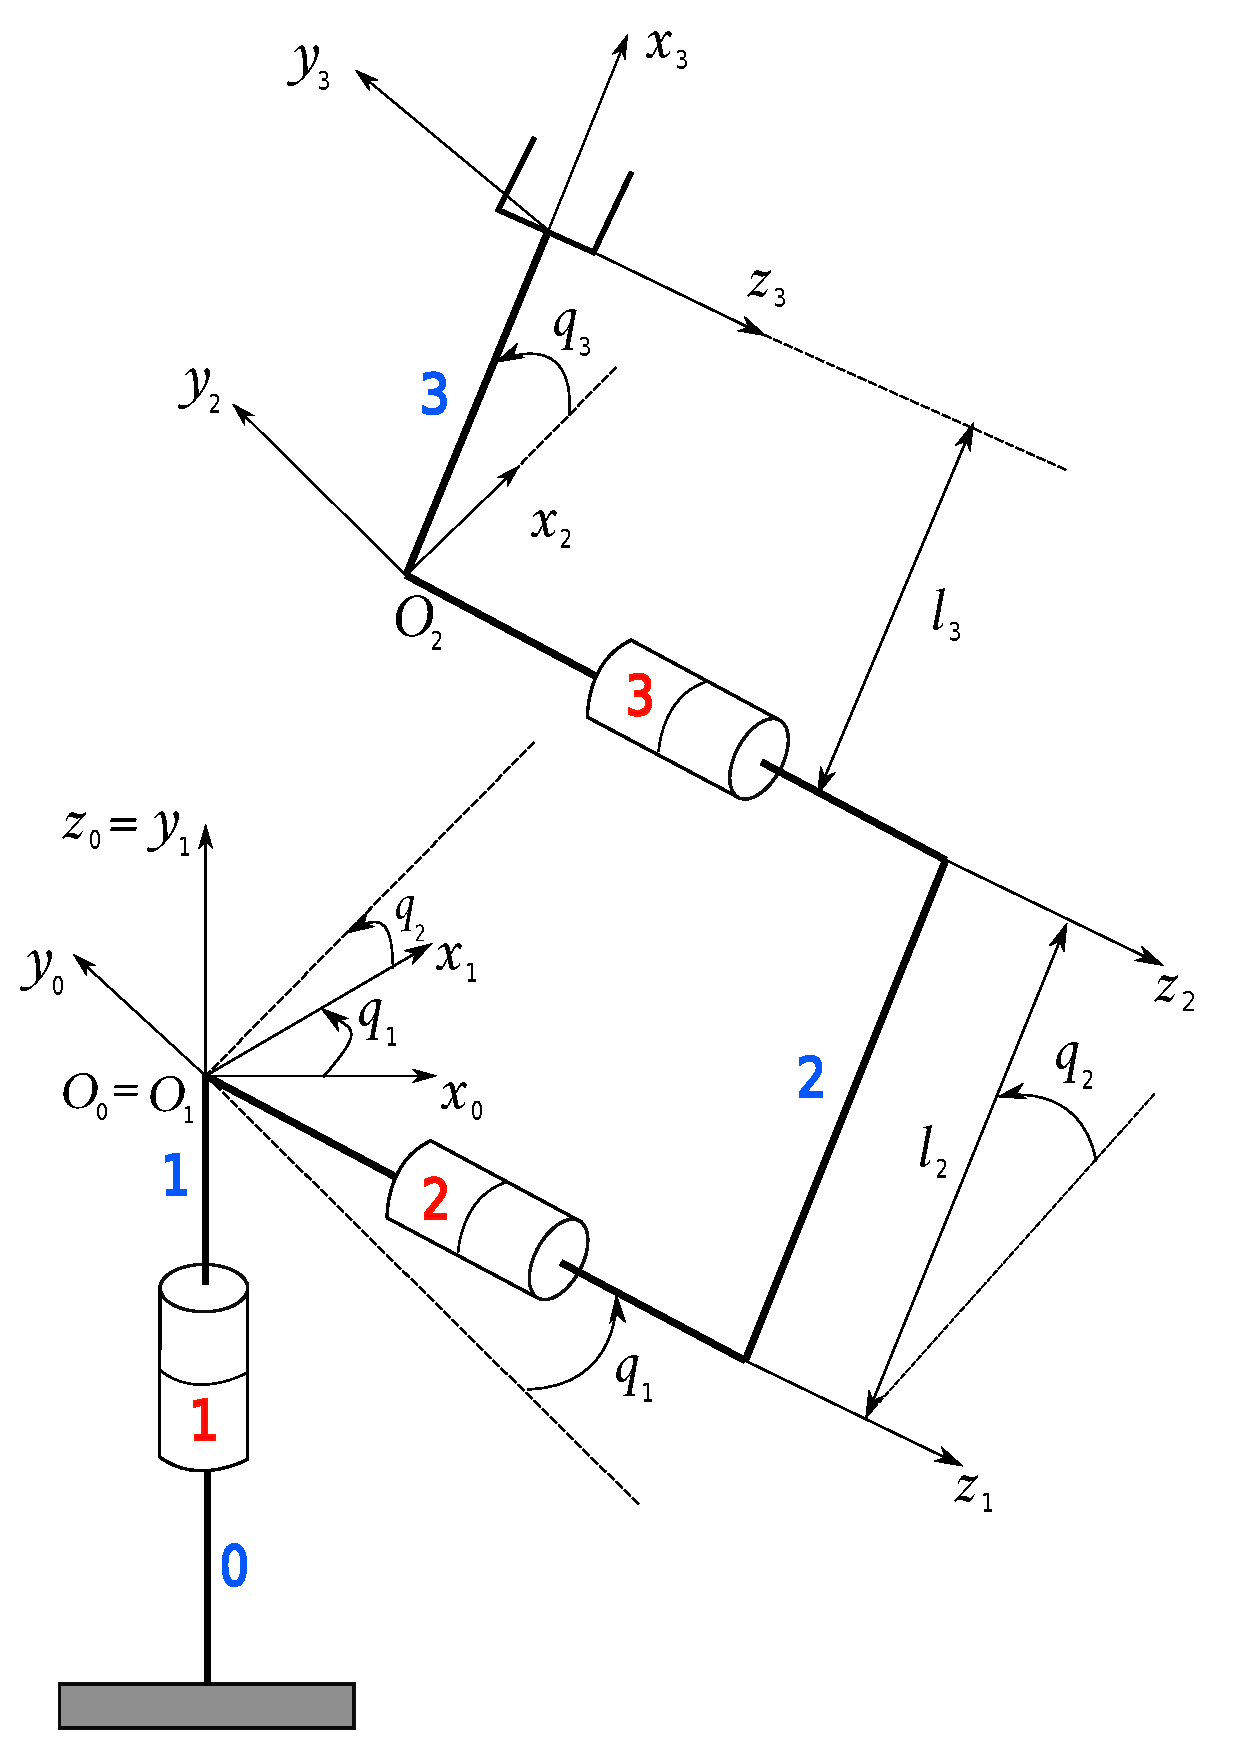
\includegraphics[scale=0.4]{manipolatoreAntropomorfo.pdf}
\captionof{figure}{Manipolatore Antropomorfo}
\end{center}

\subsubsection{Applicazione del metodo:}
Il metodo viene applicato nel modo seguente:
\begin{itemize}
	\item gli assi $z_0$, $z_1$, $z_2$ sono scelti coincidenti con gli assi dei $giunti \; 1,2,3$.
	\item l'asse $z_3$ è arbitrario e lo scegliamo parallelo agli assi $z_1$ e $z_2$
	\item l'asse $x_0$ è stato scelto ortogonale a $z_0$.
	\item gli assi $z_0$ e $z_1$ sono mutuamente ortogonali, l'asse $x_1$ è scelto in modo che $\underline{i_1} = \underline{k_0} \times \underline{k_1}$
	\item notiamo che $x_1$ sta nel piano $x_0y_0$, ovvero, piano orizzontale passante per $O_0$.
	\item dato che $z_1$ e $z_2$ sono paralleli, $x_2$ lo scegliamo passante per $O_1$
	\item scegliamo $x_3$ lungo la direzione di approccio della terna utensile
\end{itemize}


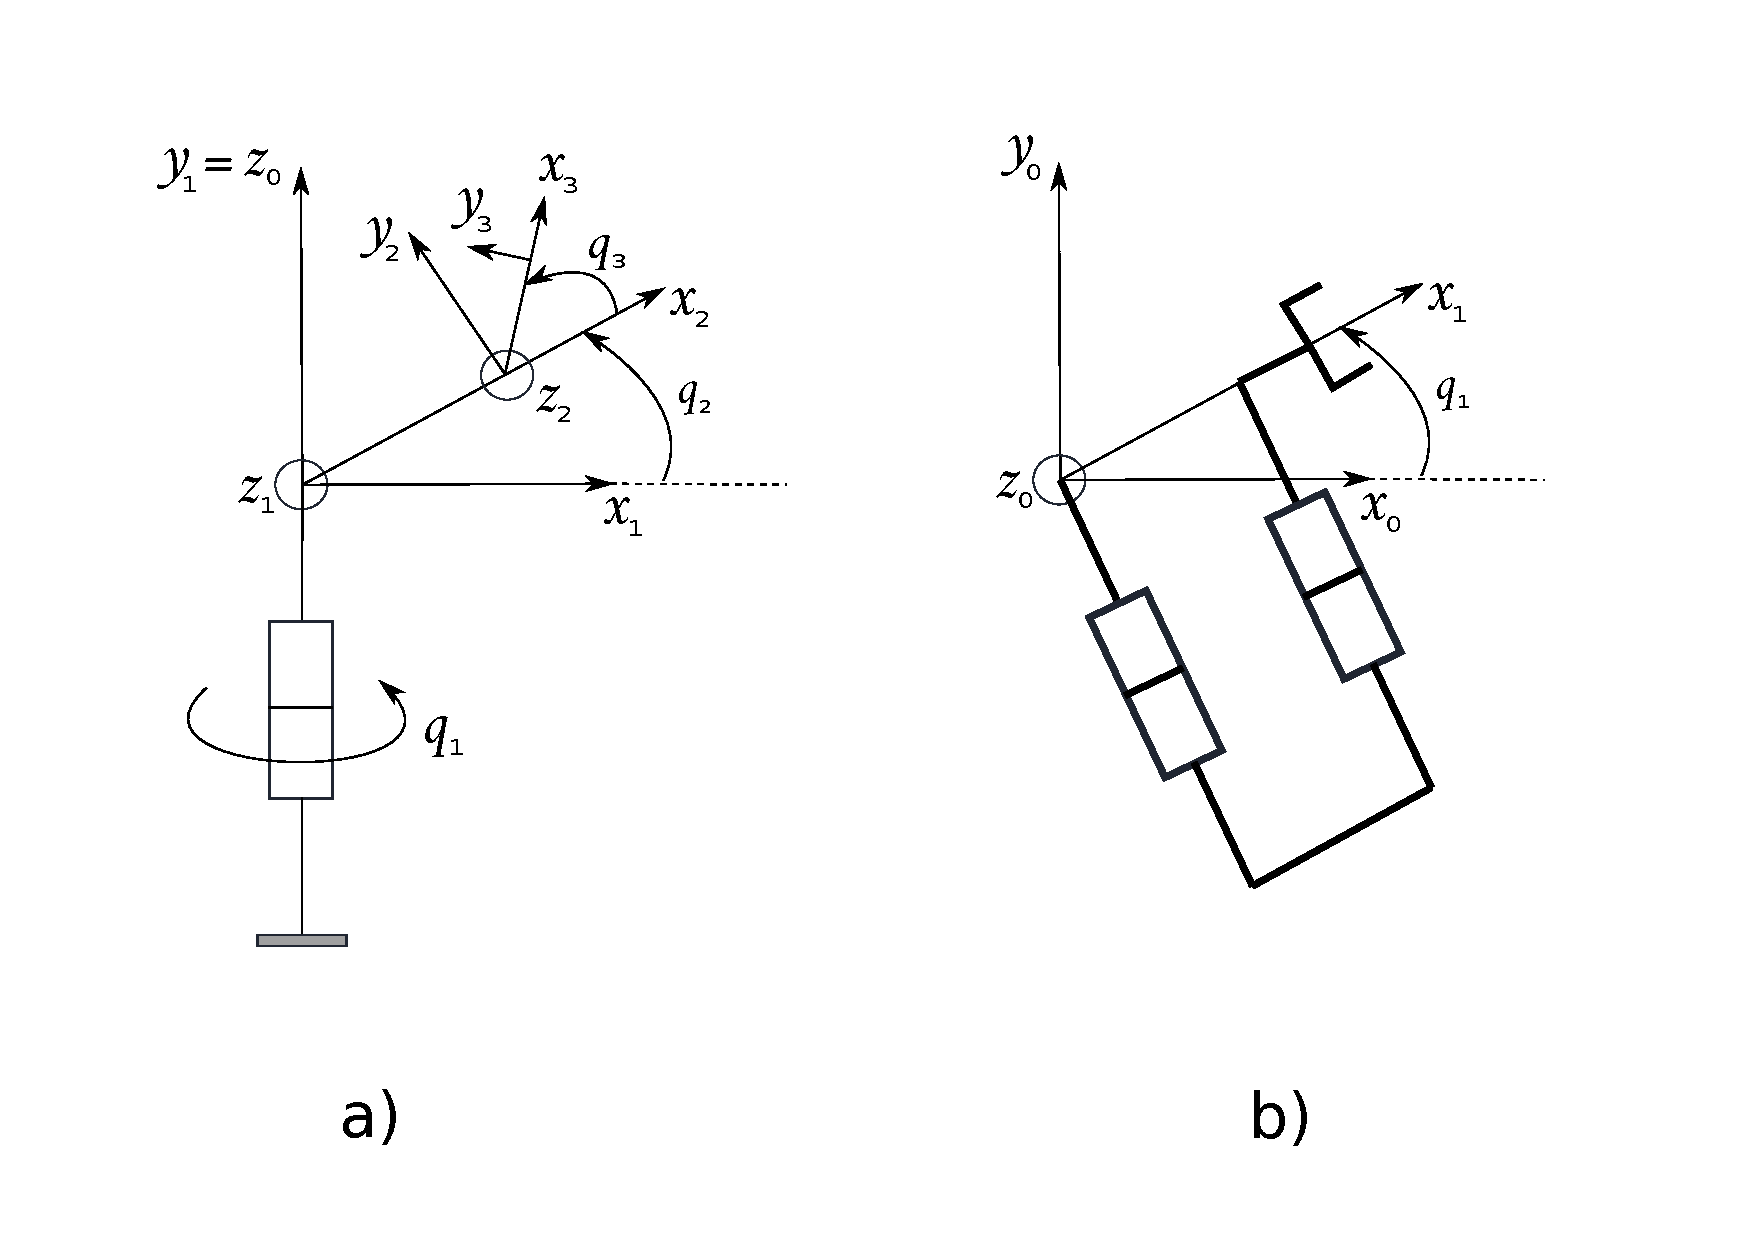
\includegraphics[scale=0.4]{visteManipolatore.pdf}
\captionof{figure}{a) vista da $z_1$  b) vista in pianta, proiezione su $x_0y_0$}

\subsubsection{Compiliamo la tabella $d_i, \theta_i, a_i, \alpha_i$:}
\begin{enumerate}
	\item $Giunto 1$:
	\begin{itemize}
		\item le origini delle terne $\langle0\rangle$ e $\langle1\rangle$ coincidono, quindi $d_1 = 0$
		\item l'asse $x_1$ si ottiene ruotando l'asse $x_0$ attorno all'asse $z_0$ di un angolo $q_1$, positivo se concorde con $z_0$
		\item la minima distanza tra $z_0$ e $z_1$ è zero, quindi $l_1 = 0$
		\item l'asse $z_1$ si ottiene ruotando l'asse $z_0$ attorno a $x_1$ di $90$, quindi $\alpha_1 = 90$
	\end{itemize}
	\item $Giunto 2$:
	\begin{itemize}
		\item $O_1$ si trova già sull'asse, quindi $d_2 = 0$
		\item l'asse $x_2$ forma rispetto all'asse $x_1$ un angolo $q_2$
		\item la minima distanza tra $z_1$ e $z_2$ è pari ad $l_1$
		\item l'asse $z_2$ è parallelo all'asse $z_1$, quindi $\alpha_2 = 0$
	\end{itemize}
	\item $Giunto 3$:
	La trasformazione dalla terna $\langle2\rangle$ alla terna $\langle3\rangle$ è sostanzialmente identica a quella dalla $\langle1\rangle$ alla $\langle2\rangle$, quindi $d_3 = 0$, $\theta_3 = q_3$ la distanza tra gli assi $z_2$ e $z_3$ è pari ad $l_3$ e $\alpha_3 = 0$.
\end{enumerate}
La tabella risulta:
\begin{center}
$
\begin{array}{|c|c|c|c|c|}
\toprule
Giunti & d_i & \theta_i & a_i & \alpha_i \\
\midrule
1 & 0 & q_1 & 0 & 90 \\
2 & 0 & q_2 & l_2 & 0 \\
3 & 0 & q_3 & l_3 & 0 \\
\bottomrule
\end{array}
$
\end{center}


\section{Polso Sferico}
Il polso sferico \emph{roll-pitch-roll} possiede 3 giunti rotoidali i cui assi si intersecano in un punto detto \emph{"centro del polso"}. 

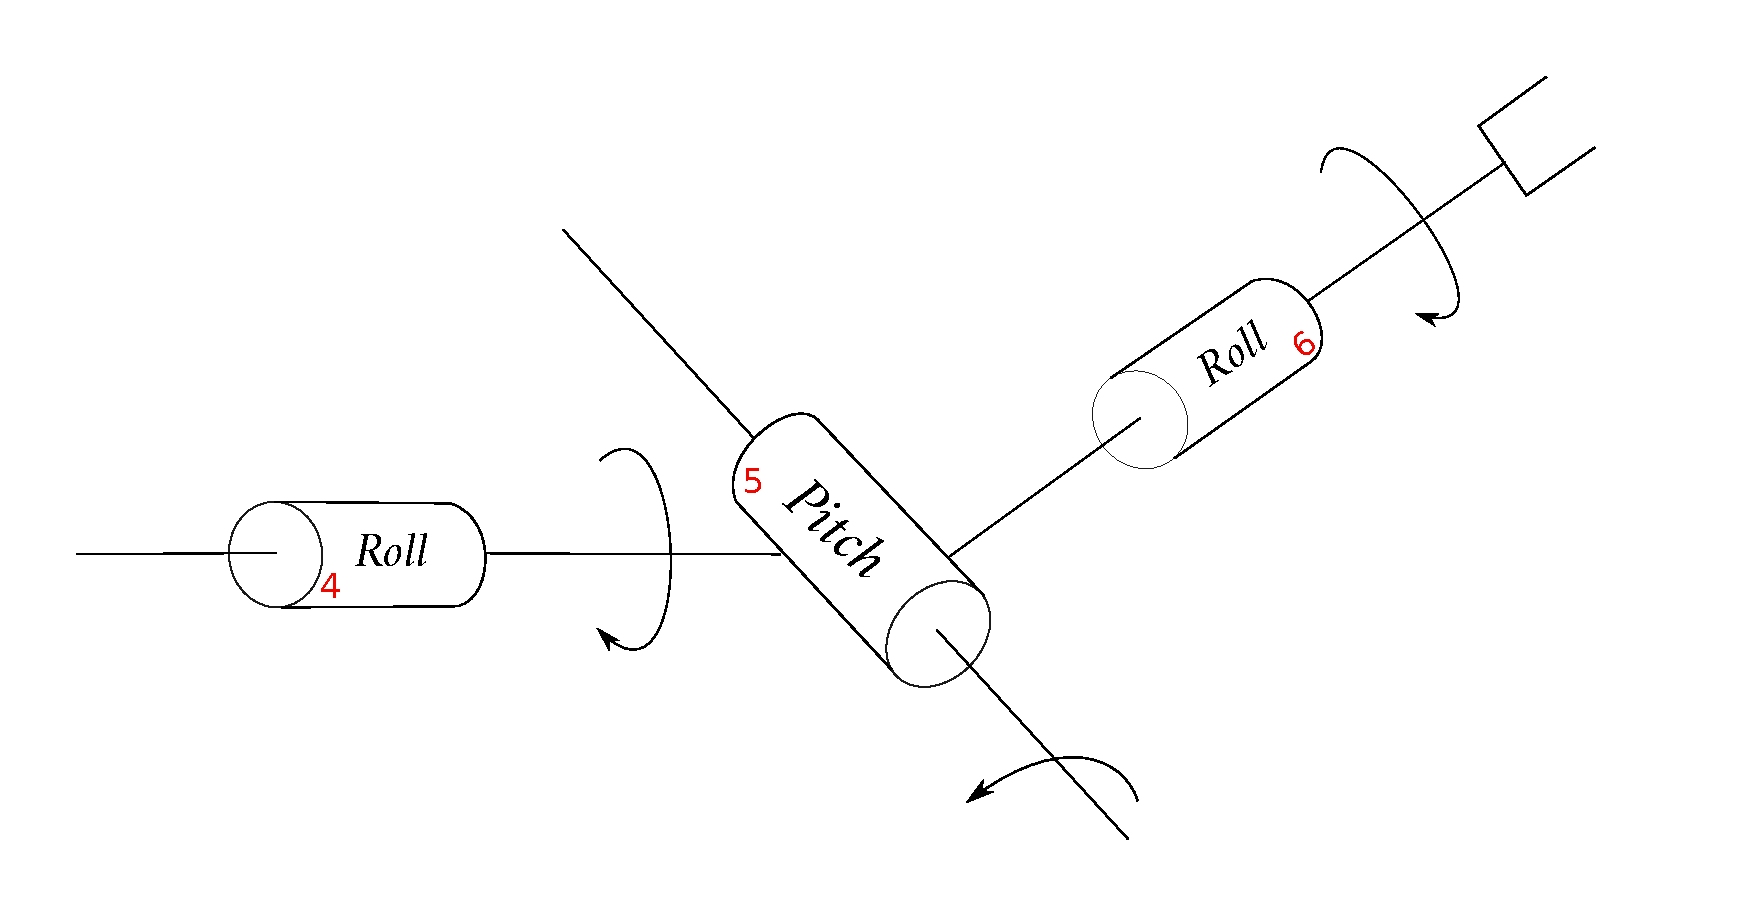
\includegraphics[scale=0.4]{polsoSferico.pdf}
\captionof{figure}{Polso sferico \emph{roll-pitch-roll}}

Esso viene utilizzato per \emph{completare} la struttura cinematica di un manipolatore a 3 DOF (che sia cilindrico, sferico o antropomorfo), consentendo di ottenere l'orientazione desiderata dell'organo terminale. Pertanto numeriamo i giunti $4$, $5$, $6$. 

\paragraph{}
Per capire la geometria del polso, disegniamolo in \emph{configurazione singolare}, ovvero con gli assi $z_3 \parallel z_5$ e notiamo:
\begin{itemize}
	\item $x_3$ normale comune a $z_2z_3$
	\item $x_4$ normale comune a $z_3z_4$
	\item $x_5$ normale comune a $z_4z_5$
	\item $x_6$ ortogonale al piano della pinza, quindi a $z_6$ 
\end{itemize}

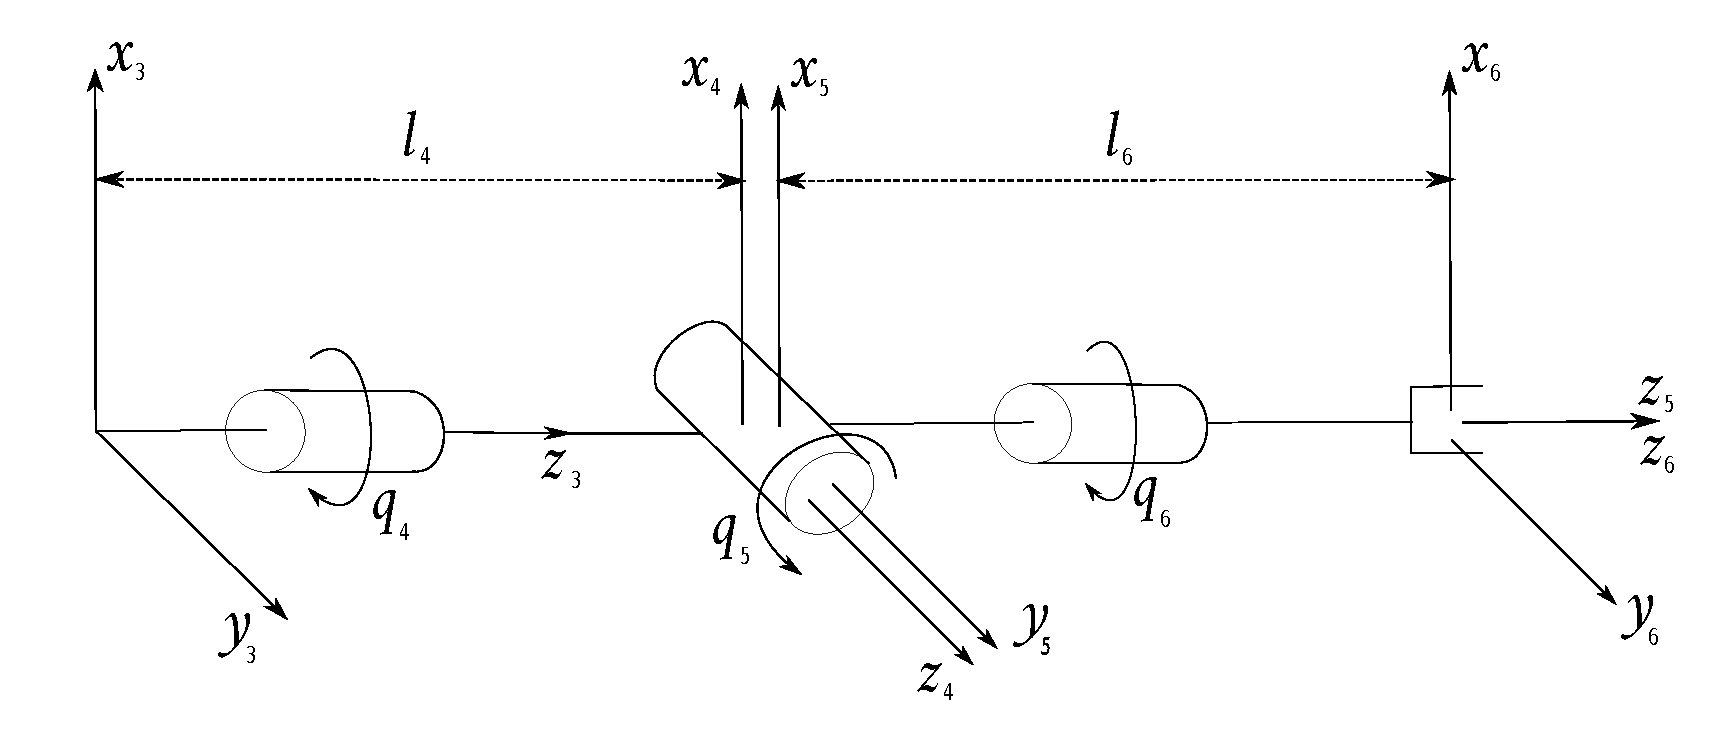
\includegraphics[scale=0.4]{polsoSfericoSingolare.pdf}
\captionof{figure}{Configurazione Singolare del polso.}

\paragraph{}
La tabella $D-H$ risulta:
\begin{center}
$
\begin{array}{ccccc}
\toprule
Giunti & d_1 & \theta_i & a_i & \alpha_i \\
\midrule
4 & l_4 & q_4 & 0 & -90 \\
5 & 0 & q_5 & 0 & 90 \\
6 & l_6 & q_6 & 0 & 0 \\
\bottomrule
\end{array}
$
\end{center}

\paragraph{}
A questo punto calcoliamo $T_i^{i-1}(d_i, \theta_i, a_i, \alpha_i)$, ovvero $T_4^3$, $T_5^4$, $T_6^5$ con \emph{intuito geometrico}. 

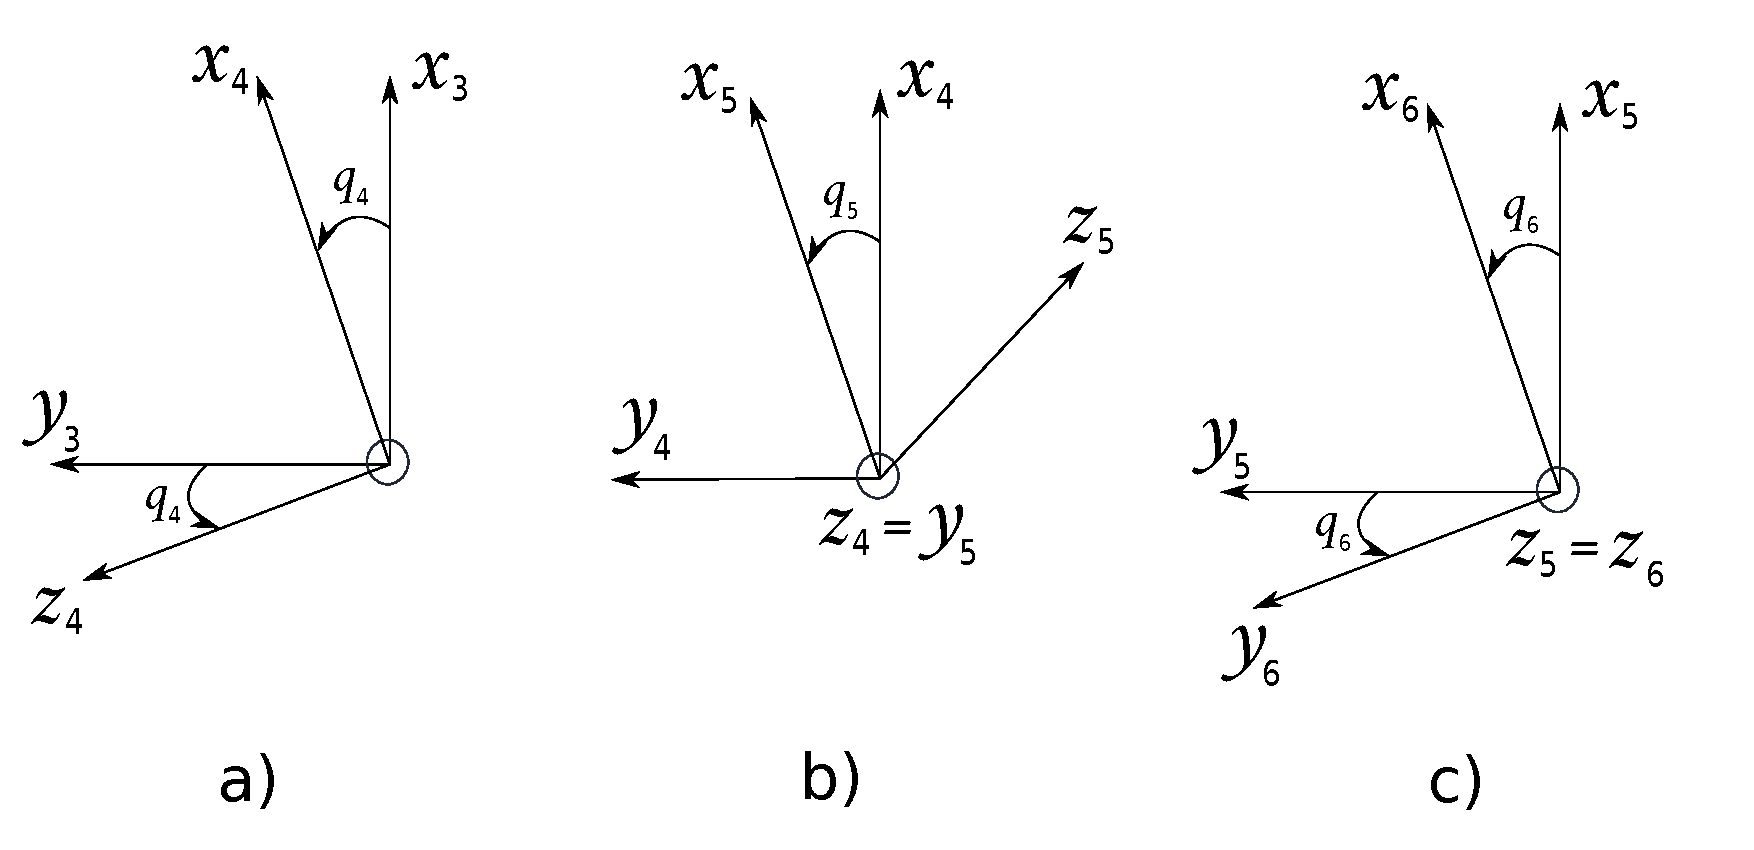
\includegraphics[scale=0.4]{polsoSfericoGeometria.pdf}
\captionof{figure}{a) vista da $z_3$ b) vista da $z_4$ c) vista da $z_5$}

\begin{equation}
	T_4^3 = 
	\begin{bmatrix}
		C_4 & 0 & -S_4 & 0 \\
		S_4 & 0 & C_4 & 0 \\
		0 & -1 & 0 & l_4 \\
		0 & 0 & 0 & 1 \\
	\end{bmatrix}
	\quad T_4^5 =
	\begin{bmatrix}
		C_5 & 0 & S_5 & 0 \\
		S_5 & 0 & -C_5 & 0 \\
		0 & 1 & 0 & 0 \\
		0 & 0 & 0 & 1 \\
	\end{bmatrix}
	\quad T_6^5 = 
	\begin{bmatrix}
		C_6 & -S_6 & 0 & 0 \\
		S_6 & C_6 & 0 & 0 \\
		0 & 0 & 1 & l_6 \\
		0 & 0 & 0 & 1 \\
	\end{bmatrix}
\end{equation}

\paragraph{}
La trasformata complessiva di polso $T_6^3$ si calcola con $R_6^3 = R_4^3\,R_5^4\,R_6^5$.

\begin{equation*}
	R_6^3 = 
	\begin{bmatrix}
		C_4 & 0 & -S_4 \\
		S_4 & 0 & C_4 \\
		0 & -1 & 0 \\
	\end{bmatrix}
	\cdot
	\begin{bmatrix}
		C_5 & 0 & S_5 \\
		S_5 & 0 & -C_5 \\
		0 & 1 & 0 \\
	\end{bmatrix}
	\cdot
	\begin{bmatrix}
		C_6 & -S_6 & 0 \\
		S_6 & C_6 & 0 \\
		0 & 0 & 1 \\
	\end{bmatrix}
	=
\end{equation*}
\begin{equation}
	= 
	\begin{bmatrix}
		C_4\,C_5\,C_6 - S_4\,S_6 & -C_4\,C_5\,S_6 - S_4\,C_6 & C_4\,S_5 \\
		S_4\,C_5\,C_6 + C_4\,S_6 & -S_4\,C_5\,S_6 + C_4\,C_6 & S_4\,S_5 \\
		-S_5\,C_6 & S_5\,S_6 & C_5 \\
	\end{bmatrix}
\end{equation}

Adesso scriviamo $R_{zyz}(\varphi,\theta,\psi)$:
\begin{equation}
	\begin{bmatrix}
		C_{\varphi}C_{\theta}C_{\psi} - S_{\varphi}S_{\psi} & -C_{\varphi}C_{\theta}C_{\psi} - S_{\varphi}S_{\psi} & C_{\varphi}S_{\theta} \\
		S_{\varphi}C_{\theta}C_{\psi} - C_{\varphi}S_{\psi} & -S_{\varphi}C_{\theta}C_{\psi} - C_{\varphi}C_{\psi} & S_{\varphi}S_{\theta} \\
		-S_{\theta}C_{\psi} & S_{\theta}S_{\psi} & C_{\theta}
	\end{bmatrix}
\end{equation}
e notiamo che otteniamo la \emph{matrice di Eulero} $zyz$ con $q_4 = \varphi$, $q_5 = \theta$, $q_6 = \psi$.
\newpage
Per completezza, mostriamo il manipolatore antropomorfo completo con il polso sferico:\\
\begin{center}
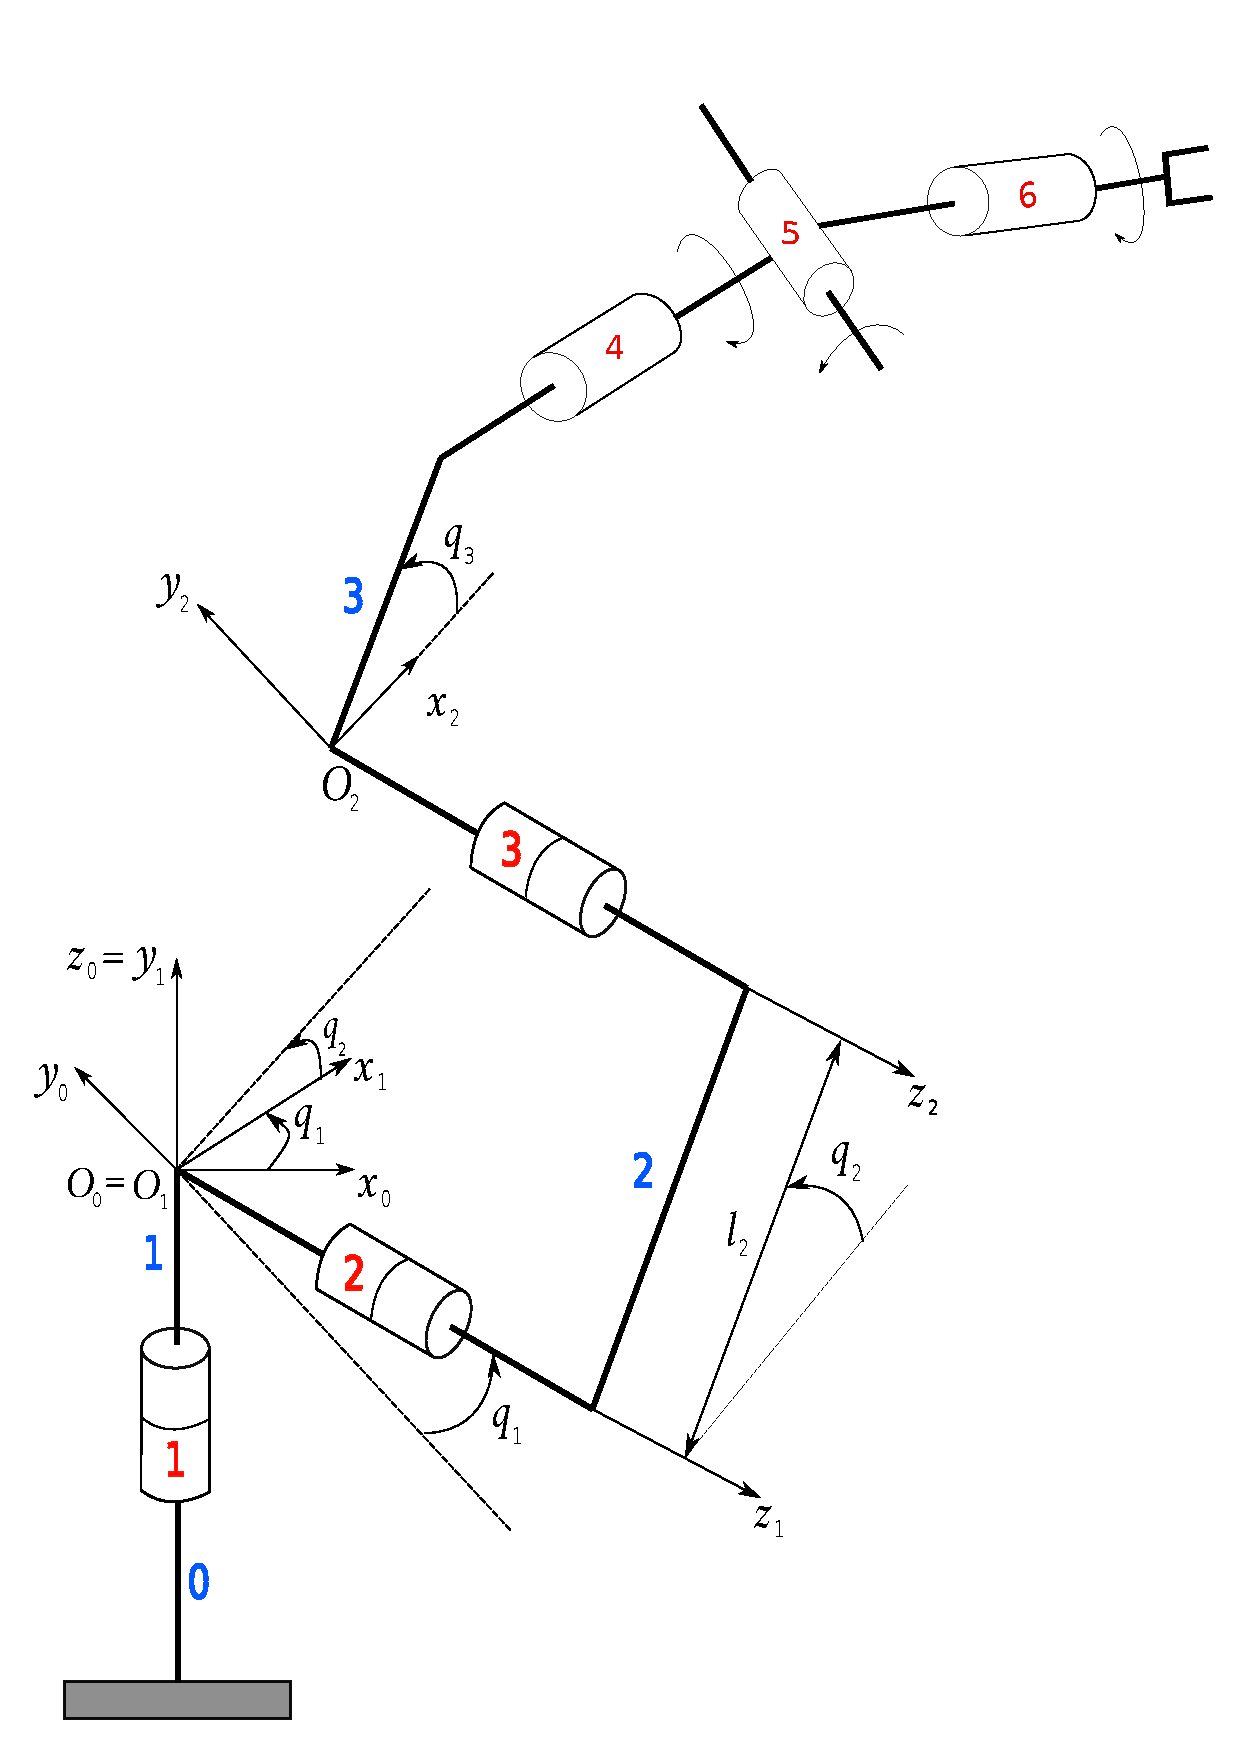
\includegraphics[scale=0.4]{manipolatoreCompleto.pdf}
\captionof{figure}{Manipolatore antropomorfo completo.}
\end{center}
\chapter{Cinematica Inversa}

Prima di iniziare questo capitolo, diamo qualche definizione:
\begin{itemize}
	\item \textbf{Spazio di Lavoro}: Regione descritta dall’origine della terna utensile quando ai giunti del manipolatore si fanno eseguire tutti i movimenti possibili.
	\item \textbf{Spazio di Lavoro Raggiungibile}: Regione dello spazio che l’origine della terna utensile può raggiungere con almeno un orientamento.
	\item \textbf{Spazio di Lavoro Destro}: regione dello spazio che l’origine della terna utensile può raggiungere con più di un orientamento.
	\item \textbf{Spazio Operativo}: Si tratta dello spazio in cui è definito il vettore $\underline{x}$. Questo spazio viene anche chiamato \emph{spazio cartesiano}.
	\item \textbf{Spazio dei Giunti}: Si tratta dello spazio in cui è definito il vettore $\underline{q}$ delle variabili di giunto. Questo spazio viene anche chiamato \emph{spazio delle configurazioni}. 
\end{itemize}

\section{Cinematica diretta e inversa}
\subsubsection{Cinematica Diretta}
Il metodo \emph{D-H} mostra come il problema cinematico diretto $KIN$ sia sempre risolvibile, ovvero, dato un vettore di coordinate di giunto $\underline{q}\in\mathbb{R}^n$, con $q_i$ grandezza lineare di $\theta_i$ (se rotoidale) o di $d_i$ (se prismatico), è sempre possibile calcolare :
\begin{itemize}
	\item la posizione $\underline{p}$ dell'origine della terna utensile (organo terminale)
	\item l'orientazione $R$ della terna utensile rispetto alla terna base
\end{itemize}
queste informazioni sono entrambe contenute nella \emph{matrice di trasformazione omogenea} $T_n^0$ che risulta essere una funzione del vettore $\underline{q}$:
\begin{equation} \label{tensore}
	T_n^0 = T_n^0(\underline{q})
\end{equation}

Nel caso in cui l'orientazione della terna utensile sia specificata in termini di angoli di Eulero (o di un'altra rappresentazione minima dell'orientazione), possiamo definire un vettore $\underline{x}\in\mathbb{R}^n$ che definisce lo \emph{spazio operativo} del robot, come segue:
\begin{equation} \label{posizione_e_orientazione}
	\underline{x} =
	\begin{bmatrix}
		\underline{p} \\
		\phi \\
	\end{bmatrix}
	\quad con \quad
	\underline{\phi} = 
	\begin{bmatrix}
		\varphi \\
		\theta \\
		\psi \\
	\end{bmatrix}
\end{equation}
dove con $\phi$ indico il vettore degli angoli di Eulero che rappresenta l'orientamento dell'organo terminale (terna utensile). 

La cinematica diretta può anche essere scritta come funzione che associa ad un vettore di coordinate di giunto $\underline{q}$ un vettore $\underline{x}$ dello spazio operativo:
\begin{equation}
	\underline{x} = \underline{x}(\underline{q})
\end{equation}

Quindi, la soluzione del problema KIN per meccanismi seriali, formulato come nella \eqref{tensore} oppure come nella \eqref{posizione_e_orientazione} ammette \emph{un'unica soluzione}, pertanto, otteniamo la seguente proposizione:

\paragraph{}
	\emph{Data una certa configurazione del meccanismo, cui è associato un vettore di coordinate di giunto $\underline{q}$, è univocamente determinata la posizione e l'orientazione dell'organo terminale e questa è data, dalla \eqref{tensore} o dalla \eqref{posizione_e_orientazione}}

\subsubsection{Cinematica Inversa}
Il problema cinematico inverso $KIN^{-1}$ consiste nel determinare possibili configurazioni nello \emph{spazio dei giunti} che forniscano una data posizione ed orientazione dell'organo terminale. Non esistono procedure standard per cercare possibili soluzioni.

In pratica, conosciamo $T_n^0$ oppure $\underline{x}$ e vogliamo calcolare delle $n-uple$ $\underline{q}$ tali che:
\begin{equation*}
	\begin{cases}
		\underline{x}(\underline{q}) = \underline{x} \quad assegnata \\
		T_n^0(\underline{q}) = T_n^0 \quad assegnata \\
	\end{cases}
\end{equation*}

Il problema $KIN^{-1}$ risulta più complesso perchè dato un certo meccanismo, possono esistere o meno soluzioni e, se esistono soluzioni, queste possono essere in numero finito o infinito.

Supponiamo di avere una orientazione desiderata $R_{des}$ e una posizione desiderata $\underline{p}_{\,des}$, possono accadere tre cose:
\begin{enumerate}
	\item $R_{des}$, $\underline{p}_{\,des}$ non appartengono allo spazio di lavoro $\Rightarrow$ $0$ soluzioni.
	\item $R_{des}$, $\underline{p}_{\,des}$ appartengono allo spazio di lavoro, ma ci sono infiniti modi di risolvere il problema $\Rightarrow$ $\infty$ soluzioni.
	\item $R_{des}$, $\underline{p}_{\,des}$ appartengono allo spazio di lavoro e vi è un numero preciso di soluzioni del problema $\Rightarrow$ $\exists$ un numero finito di soluzioni.
\end{enumerate}
\newpage

\section{Esempi manipolatori planari}
Consideriamo il caso planare, la posizione e l'orientazione dell'organo terminale (pinza) possono essere specificate con tre parametri ($p_x$, $p_y$, $\phi$). Vediamo gli esempi:

\subsubsection{Robot planare 2R}
Un robot seriale 2R (con due giunti rotoidali) può raggiungere la posizione desiderata $\underline{p}$ in due modi possibili: \emph{elbow up} (gomito alto) e \emph{elbow down} (gomito basso). Una volta scelte le coordinate di giunto $q_1$ e $q_2$ in modo da soddisfare la specifica posizionale, l'orientazione dell'organo terminale $\phi$ è fissata e quindi non possiamo scegliere arbitrariamente l'orientazione e pertanto l'orientazione desiderata non è soddisfatta. Notiamo che il punto $\underline{p}$ appartiene allo \emph{spazio di lavoro destro} perchè è raggiungibile con due orientazioni. 

Pertanto la soluzione al problema cinematico inverso è una sola, ovvero, quella disegnata sotto che soddisfa l'orientazione e la posizione. Ma non ne posso trovare altre perchè ruotando i giunti, l'orientazione cambia.

\begin{center}
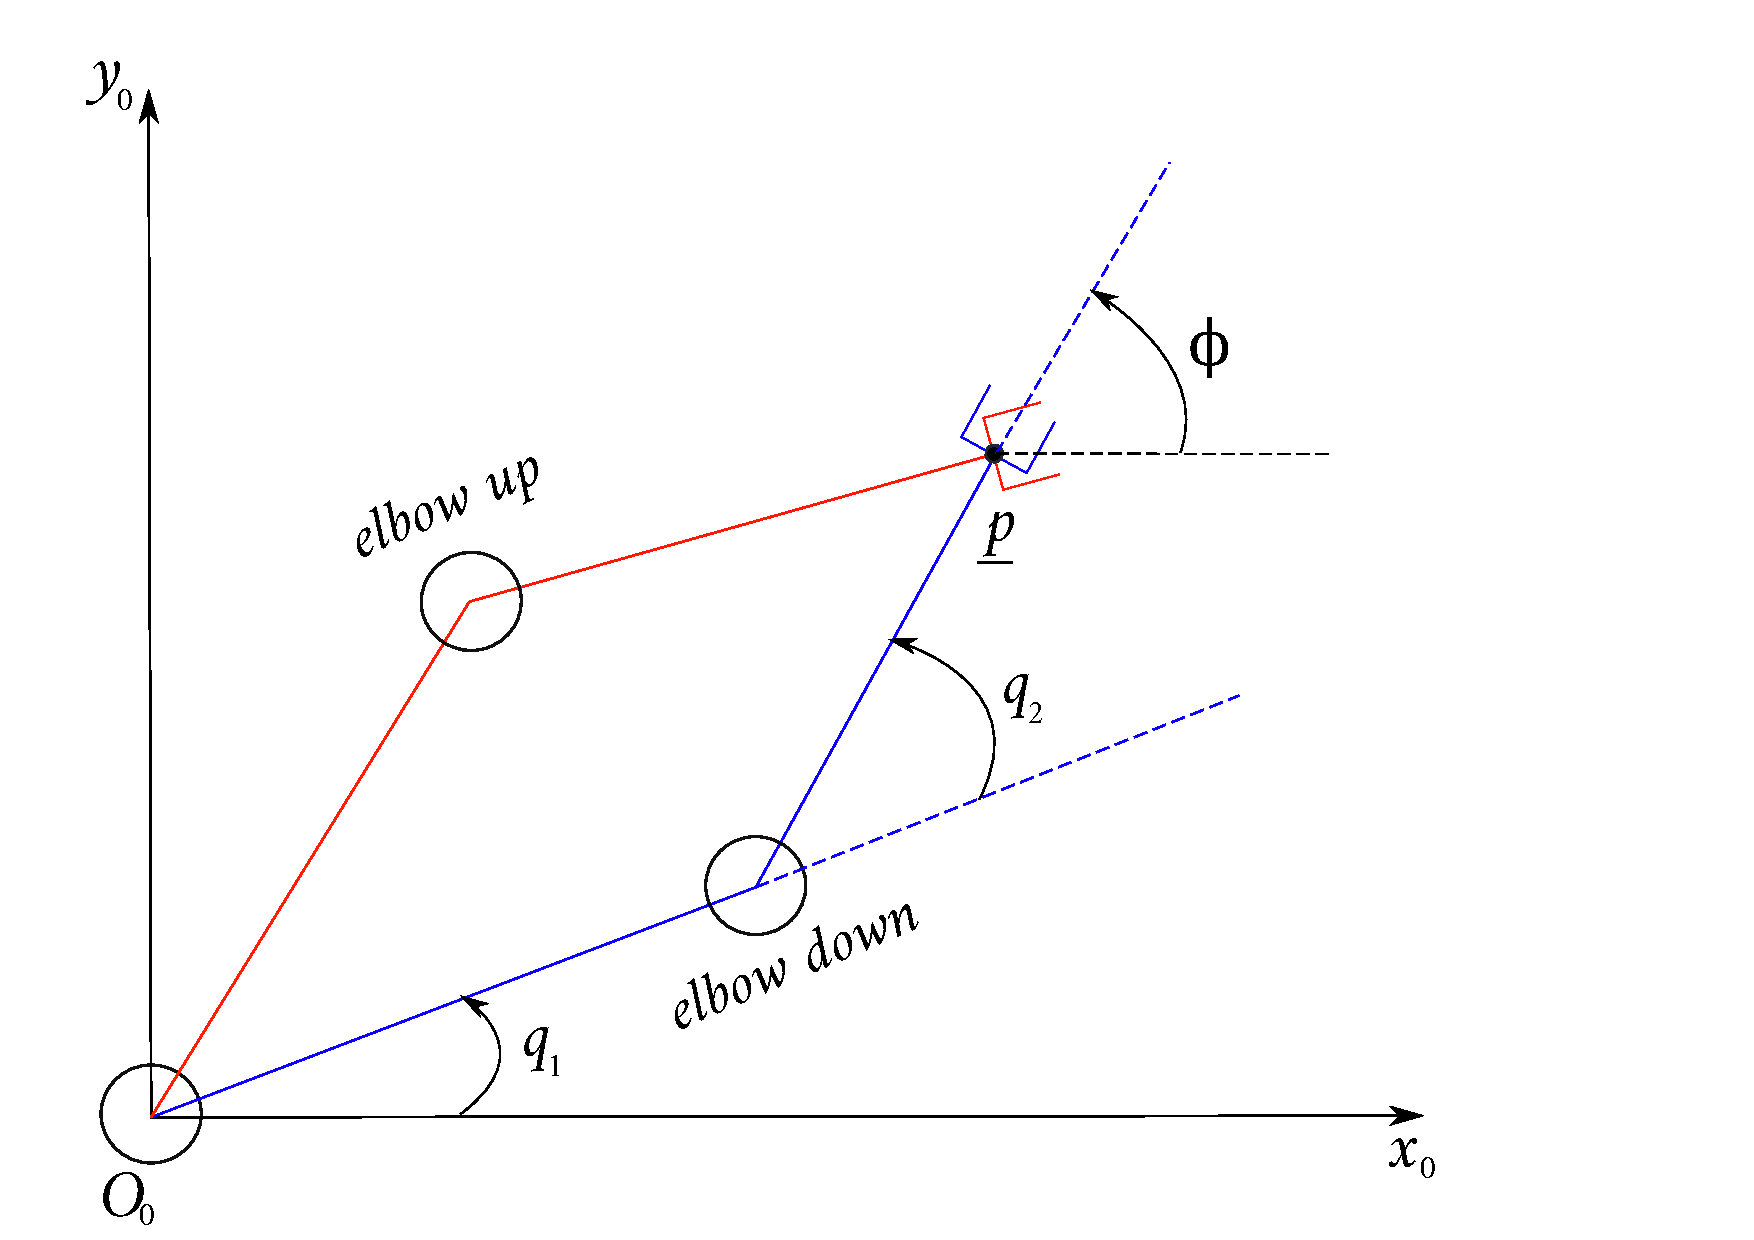
\includegraphics[scale=0.3]{manipolatoreInverso2R.pdf}
\captionof{figure}{Manipolatore planare 2R.}
\end{center}

\subsubsection{Robot planare 3R}
In un robot planare 3R è possibile soddisfare sia la specifica posizionale che la specifica dell'orientazione. Le soluzioni possibili sono due.

\begin{center}
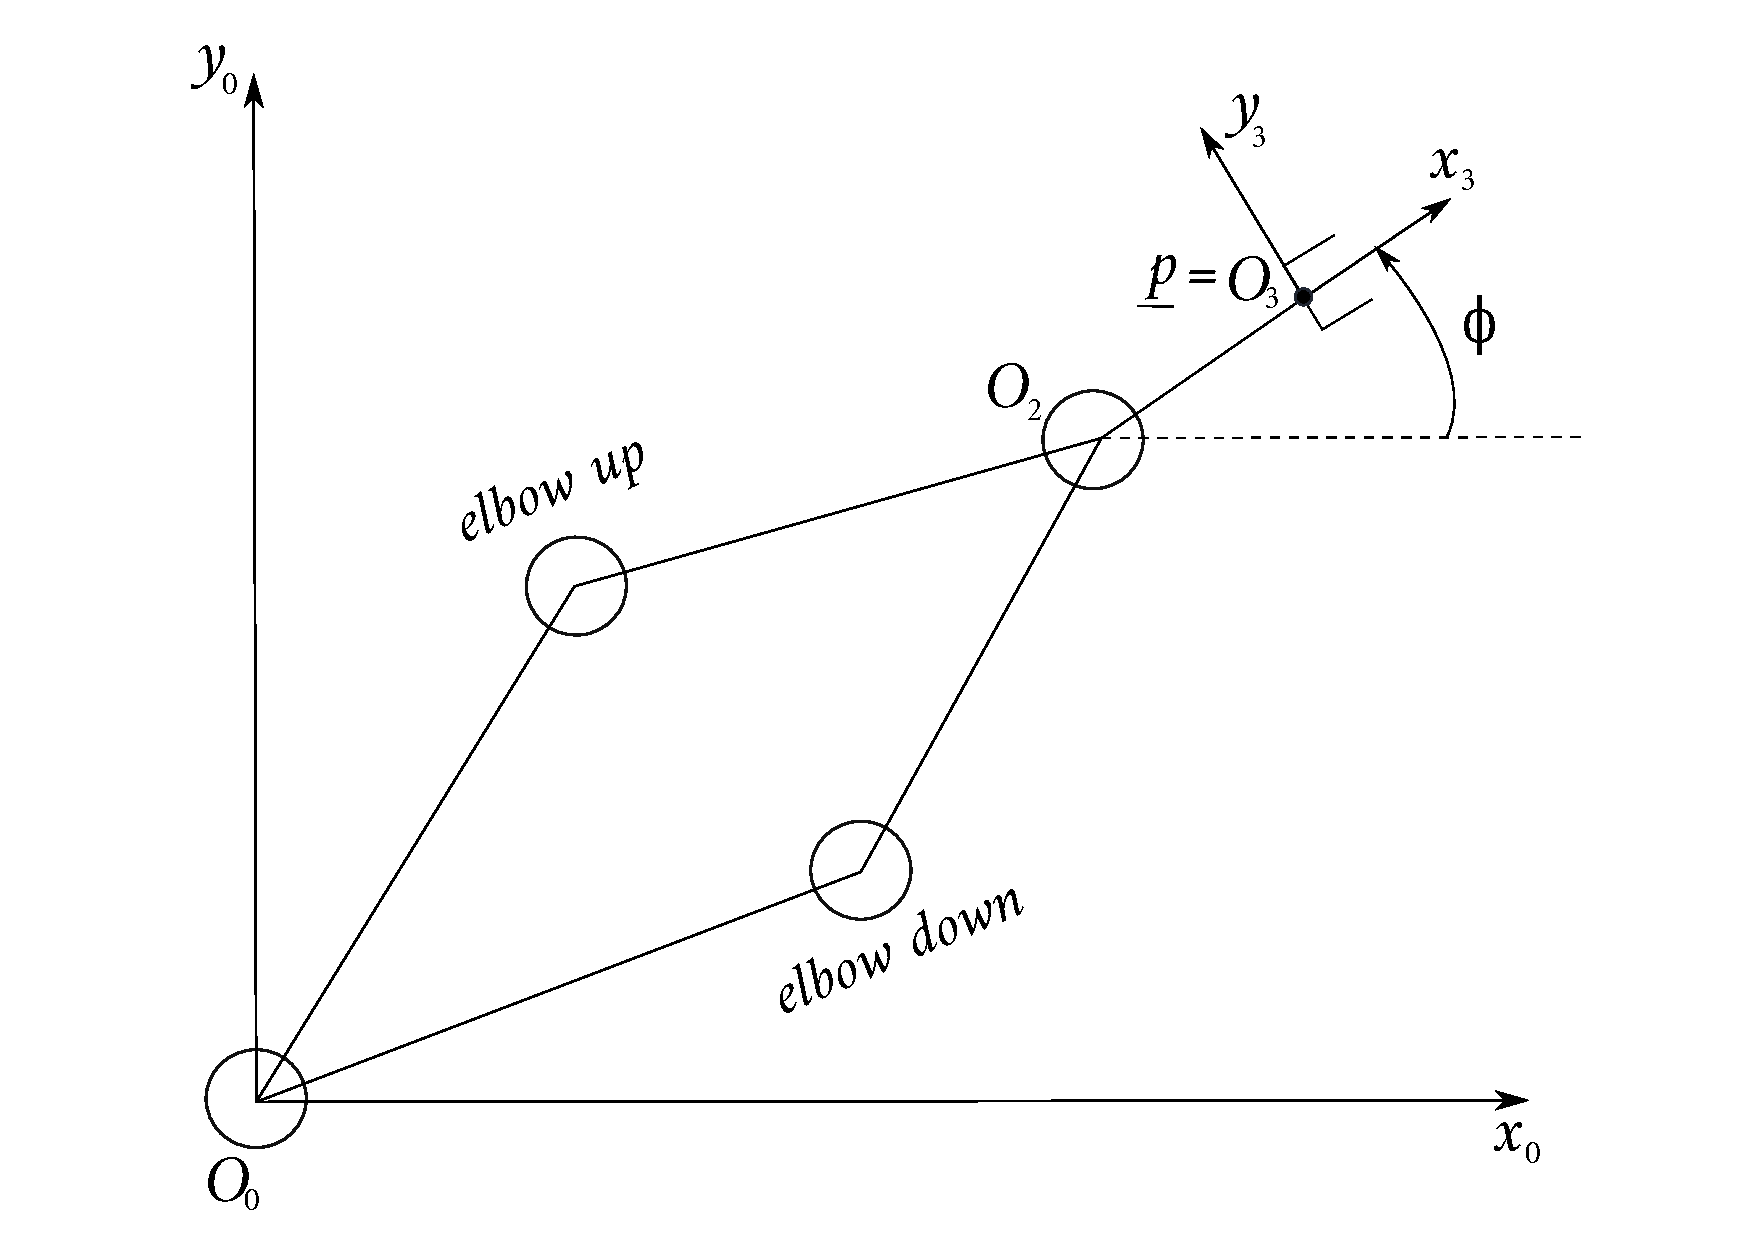
\includegraphics[scale=0.3]{manipolatoreInverso3R.pdf}
\captionof{figure}{Manipolatore planare 3R.}
\end{center}

Troviamo $\underline{q} = [q_1 \; q_2 \; q_3]^T$ che soddisfa la specifica di posa $\underline{p}$, $\phi$. Semplifichiamo il problema eliminando la terza coordinata posizionale e consideriamo $\underline{w}$ come in figura ($3.3$a).

\begin{center}
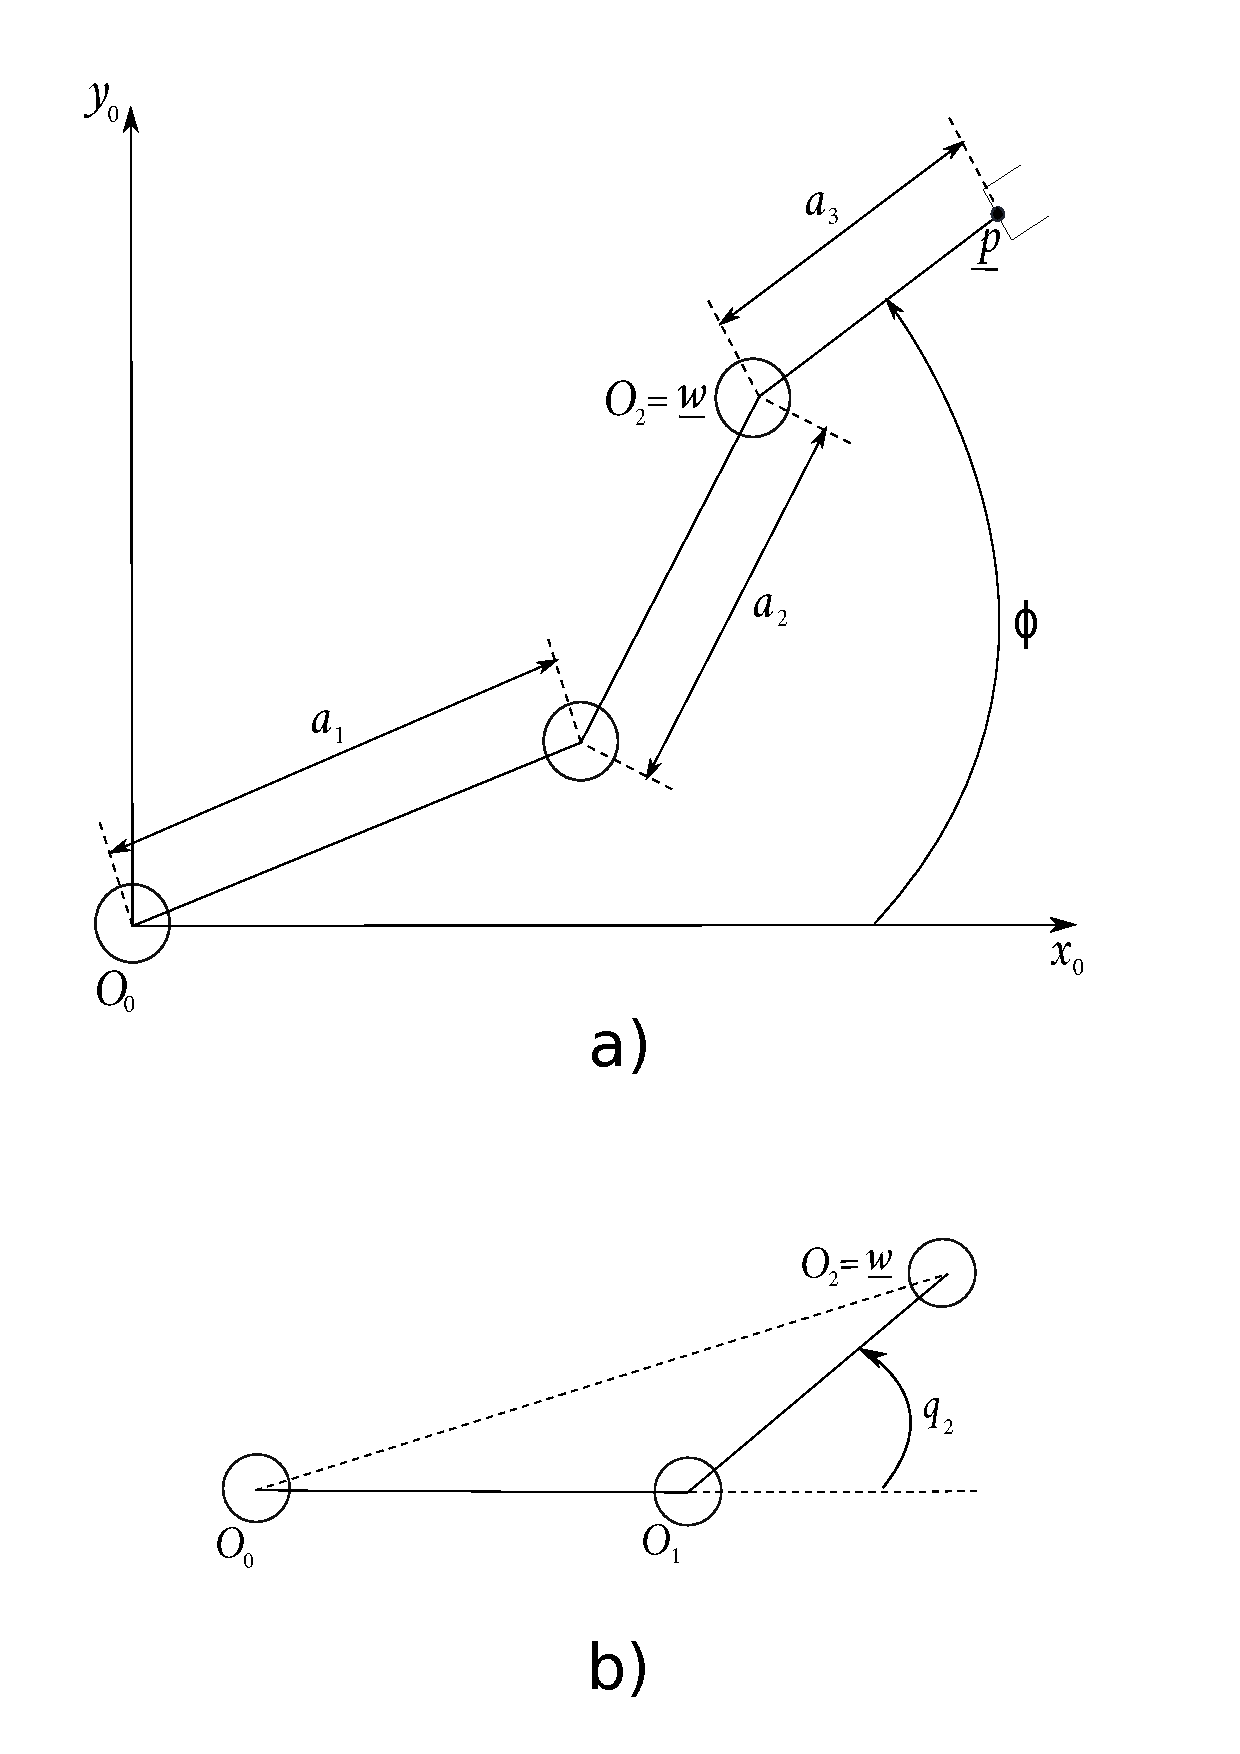
\includegraphics[scale=0.3]{manipolatoreInverso3RGeometria.pdf}
\captionof{figure}{a) Geometria del manipolatore 3R b) Triangolo $OO_1\underline{w}$ }
\end{center}

Quindi, abbiamo la seguente espressione per $\underline{O_2} = \underline{w}$:
\begin{equation*}
	\underline{w} = \underline{p} - a_3\,\underline{i_3} = \underline{p}-a_3
	\begin{bmatrix}
		C_{\phi} \\
		S_{\phi} \\
		0 \\
	\end{bmatrix}
\end{equation*}

Per calcolare $q_1$ e $q_2$ procediamo risolvendo il problema $KIN$ per trovare $\underline{x}$:

\begin{equation*}
	KIN:
	\begin{cases}
		p_x = a_1C_1 + a_2C_{12} + a_3C_{123} \\
		p_y = a_1S_1 + a_2S_{12} + a_3S_{123} \\
		\phi = q_1 + q_2 + q_3 \\
		con \; C_{123} = C_{\phi} \; e \; S_{123} = S_{\phi} \\
	\end{cases} \quad\Rightarrow\quad \underline{x} = 
	\begin{bmatrix}
		p_x \\
		p_y \\
		\phi \\
	\end{bmatrix}
\end{equation*}

quindi otteniamo:
\begin{equation} \label{wx_wy}
	\begin{cases}
		w_x = p_x - a_3C_{\phi} = a_1C_1 + a_2C_{12} \\
		w_y = p_y - a_3S_{\phi} = a_1S_1 + a_2S_{12} \\
	\end{cases}
\end{equation}
A questo punto, per trovare $q_1$ e $q_2$ possiamo procedere per via \emph{algebrica} o per via \emph{geometrica}.

\paragraph{}
Procediamo per via geometrica utilizzando il \emph{teorema di Carnot} per il triangolo in figura 3.3b:
\begin{equation}
	\overline{Ow}^2 = (a_1)^2 + (a_2)^2 - 2a_1a_2\,\cos(\pi - q_2)
\end{equation}

e otteniamo,
\begin{equation*}
	w_x^2 + w_y^2 = (a_1)^2 + (a_2)^2 + 2a_1a_2\,\cos(q_2)
\end{equation*}

pertanto,
\begin{equation*}
	\Rightarrow \quad 
	\cos(q_2) = \dfrac{w_x^2 + w_y^2 - (a_1)^2 - (a_2)^2}{2a_1a_2}
\end{equation*}

esistono due rami di soluzione,
\begin{align}
	q_2 = atan_2(\sqrt{1-C_2^2}, C_2) \\
	q_2 = atan_2(-\sqrt{1-C_2^2}, C_2)
\end{align}
abbiamo trovato la coordinata di giunto $q_2$.

\paragraph{}
Per trovare le altre coordinate di giunto riprendiamo la \eqref{wx_wy} e considerando $C_{12} = \cos(q_1 + q_2) = C_1C_2 - S_1S_2$ e $S_{12} = \sin(q_1 + q_2) = S_1C_2 + S_2C_1$,
\begin{equation}
	\begin{cases}
		w_x = p_x - a_3C_{\phi} = a_1C_1 + a_2(C_1C_2 - S_1S_2) \\
		w_y = p_y - a_3S_{\phi} = a_1S_1 + a_2(S_1C_2 + S_2C_1) \\
	\end{cases}
\end{equation}

in questo sistema lineare le incognite sono solo $S_1$ e $C_1$ e pertanto scrivo:
\begin{equation}
	\begin{bmatrix}
		w_x \\
		w_y \\
	\end{bmatrix}
	=
	\begin{bmatrix}
		a_1 + a_2C_2 & -a_2S_2 \\
		a_2S_2 & a_1 + a_2C_2 \\ 
	\end{bmatrix}
	\cdot
	\begin{bmatrix}
		C_1 = \cos(q_1) \\
		S_1 = \sin(q_1) \\
	\end{bmatrix}
\end{equation}

e ottengo,
\begin{equation}
	\begin{cases}
		q_1 = atan_2(S_1, C_1) \\
		q_2 = equazione\;(3.6) \\
		q_3 = \phi - q_1 - q_2 \\
	\end{cases}
\end{equation}
	
\subsubsection{Robot planare 4R}
Se abbiamo un robot planare 4R, è possibile soddisfare la specifica posizionale e quella di orientazione e le soluzioni possibili saranno $\infty$, infatti il 4R è cinematicamente ridondante (nel piano) perchè dato un punto $\underline{p}$, possiamo raggiungerlo in infiniti modi (infinite configurazioni).

\begin{center}
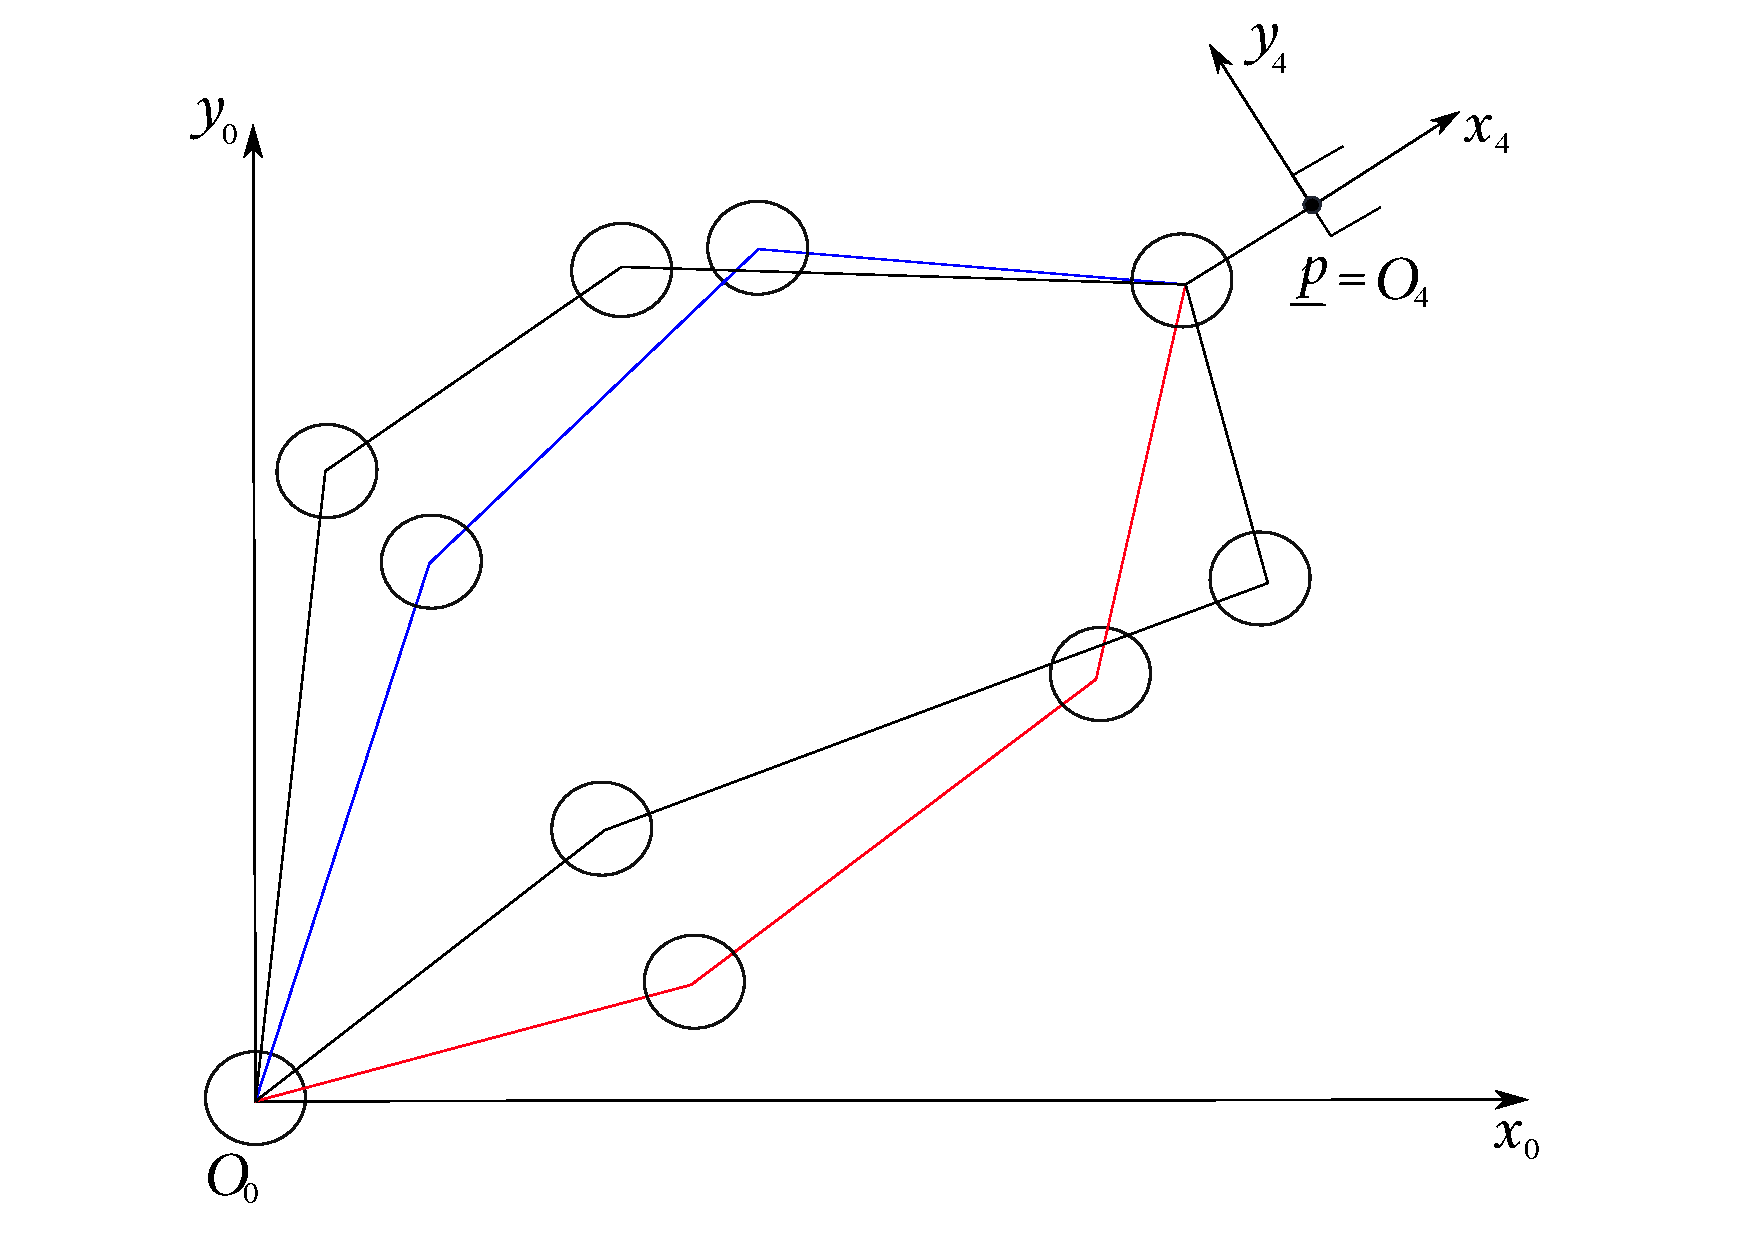
\includegraphics[scale=0.3]{manipolatoreInverso4R.pdf}
\captionof{figure}{Possibili configurazioni del manipolatore 4R}
\end{center}

\section{$KIN^{-1}$ di manipolatori con polso sferico}
Adesso esaminiamo un manipolatore spaziale. Pieper dimostrò che:
\paragraph{}
\emph{Per ogni manipolatore a 6 DOF in cui esistono tre giunti adiacenti con assi che si intersecano in un unico punto, allora la soluzione del problema cinematico inverso esiste in forma chiusa.}
\paragraph{}
Un particolare tipo di struttura con tre assi di giunti adiacenti che si intersecano in un punto è il giunto sferico (polso) di tipo roll-pitch-roll mostrato in figura.

\begin{center}
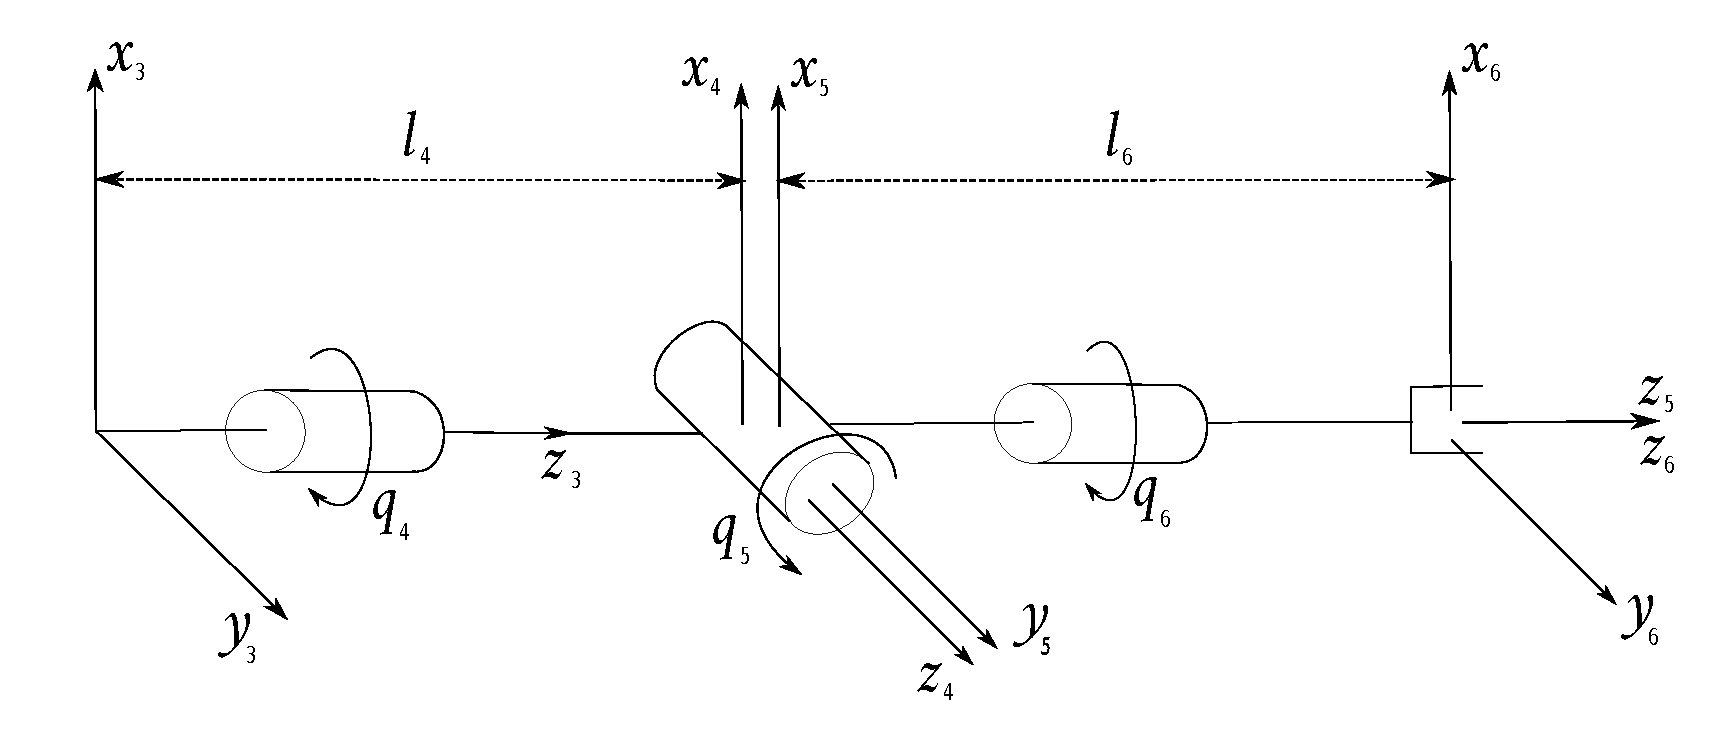
\includegraphics[scale=0.225]{polsoSfericoSingolare.pdf}
\captionof{figure}{Configurazione Singolare del polso $z_5 \parallel z_6$} 
\end{center}

\paragraph{}
Il manipolatore completo a 6 DOF (figura $2.8$) composto da una struttura di manipolazione a 3 DOF più un polso sferico anch'esso a 3 DOF soddisfa ancora la \emph{condizione di Pieper}. 

Possiamo definire un \emph{"metodo generale per $KIN^{-1}$ di manipolatori con polso sferico"}. Iniziamo scrivendo i \emph{dati del problema}:
\begin{itemize}
	\item $\underline{p} = \underline{O_6}$ 
	\item $R = R_6^0$
\end{itemize}

\paragraph{}
Possiamo suddividere il problema a 6 DOF in due sottoproblemi più semplici a 3 DOF ciascuno. Una volta nota la posizione e l'orientazione desiderata dell'organo terminale, la posizione del \emph{centro del polso} $\underline{w}$ è calcolabile come segue:
\begin{equation} \label{w_polso}
	\underline{w} = \underline{p} - l_6\,\underline{k_5}
\end{equation}

e la posizione del centro del polso dipende solo dalle coordinate dei primi tre giunti del robot:
\begin{equation} \label{funzione_w}
	\underline{w} = \underline{w}(q_1, q_2, q_3)
\end{equation}
notiamo che la \eqref{w_polso} rappresenta il calcolo di $\underline{w}$ in funzione dei dati del problema e che $\underline{k_5} = \underline{k_6}$ è la terza colonna di $R = R_6^0$

\paragraph{}
Quindi si può risolvere in modo agevole il problema della cinematica inversa della struttura di manipolazione, ottenendo $q_1$, $q_2$, $q_3$ dalla \eqref{funzione_w}, scriviamo i passi:
\begin{enumerate}
	\item[1)] Calcolare $q_1$, $q_2$, $q_3$ tali che: $\underline{w}(q_1, q_2, q_3) = \underline{p} - l_6\,\underline{k_5} = \underline{w}_{\,des}$
	\item[2)] Calcolare $q_4$, $q_5$, $q_6$ tali che: $R_3^0(q_1, q_2, q_3) \cdot R_6^3(q_4, q_5, q_6) = R$
	\begin{enumerate}
		\item[2.1)] noti $q_1$, $q_2$, $q_3$ dalla $KIN^{-1}$, calcolo $R_3^0(q_1, q_2, q_3)$
		\item[2.2)] avendo calcolato $R_3^0$ e avendo $R$ noto (come dato del problema) calcolo $R_3^0\,R_6^0 = R \Rightarrow R_6^3 = (R_3^0)^T\,R$
		\item[2.3)] avendo calcolato $R_6^3$ posso calcolare $R_6^3 = R_6^3(q_4, q_5, q_6)$ per trovare $q_4$, $q_5$, $q_6$ è possibile utilizzare le formule di inversione della \emph{matrice di Eulero}, infatti, posso scrivere:
		\begin{equation}
			R_6^3(q_4, q_5, q_6) = R_{zyz}(\varphi, \theta, \psi) \quad con 
			\begin{cases}
				\varphi = q_4 \\
				\theta = q_5 \\
				\psi = q_6 \\
			\end{cases}
		\end{equation}
	\end{enumerate}
\end{enumerate}
\chapter{Cinematica Differenziale}
Fino adesso, abbiamo esaminato il problema della \emph{cinematica diretta} posizionale e successivamente \emph{l'inversione} della cinematica diretta. La \emph{cinematica differenziale} riguarda la derivazione della relazione che esiste tra le velocità dei giunti ed il moto dell'organo terminale (inteso come velocità di traslazione di un suo punto e velocità angolare).

\begin{align}
	KIN: \quad \underline{q} \longrightarrow \underline{p}, R \;(oppure\; \underline{p}, \underline{\phi}) \\
	\dot{KIN}: \quad \dot{\underline{q}} \longrightarrow \dot{\underline{p}}, \underline{\omega}\;(oppure\; \dot{\underline{p}}, \dot{\underline{\phi}})
\end{align}
	
\subsubsection{Cinematica diretta}
Nella trattazione della cinematica diretta si fissa una terna sull'organo terminale e si ricava la relazione tra le coordinate di giunto e la matrice di trasformazione omogenea $T_n^0$. In alternativa si può cercare la relazione esistente tra le coordinate di giunto ed il vettore $\underline{x}$ che definisce la posizione dell'organo terminale nello spazio operativo.

\subsubsection{Cinematica Differenziale}
Nello studio della cinematica differenziale bisogna invece cercare il legame tra le derivate temporali delle coordinate di giunto e la velocità della terna utensile, fissata all'organo terminale.

\section{Jacobiano Analitico}
Per tracciare la \emph{posizione} dell'organo terminale usiamo il \emph{vettore dello spazio operativo} $\underline{x}$ e derivando otteniamo il \emph{vettore velocità nello spazio operativo} $\dot{\underline{x}}$:

\begin{equation}
	\underline{x} = 
	\begin{bmatrix}
		\underline{p} \\
		\underline{\phi} \\
	\end{bmatrix}
	\qquad \dot{\underline{x}} = 
	\begin{bmatrix}
		\dot{\underline{p}} \\
		\dot{\underline{\phi}} \\
	\end{bmatrix}
\end{equation}

indicando con $\underline{p}$ posizione dell'origine della terna utensile e $\underline{\phi}$ una rappresentazione minima dell'orientazione.

Sia $\underline{f}$ la funzione $KIN$, consideriamo $\underline{x} = f(\underline{q})$ e definiamo la derivata del \emph{vettore dello spazio operativo} come segue:
\begin{equation}
	\dot{\underline{x}} =   \frac{\partial \underline{f}(\underline{q})}{\partial \underline{q}} \cdot \underline{\dot{q}}
\end{equation}

\paragraph{}
A questo punto, definiamo lo \emph{Jacobiano Analitico}, ovvero la \emph{matrice Jacobiana} $J_{a}$, come:
\begin{equation}
	J_a(\underline{q}) = \frac{\partial \underline{f}(\underline{q})}{\partial \underline{q}}
\end{equation}

pertanto possiamo scrivere:
\begin{equation}
	\dot{\underline{x}} = J_a(\underline{q}) \cdot \dot{\underline{q}} \quad \Rightarrow \quad 
	\begin{cases}
		\dot{\underline{p}} = J_{ap}(\underline{q})\,\underline{\dot{q}} \\
		\dot{\underline{\phi}} = J_{ao}(\underline{q})\,\dot{\underline{q}} \\
	\end{cases} 
\end{equation}

dove $J_{ap}$ e $J_{ao}$ sono le due sottomatrici ($\in\mathbb{R}^{3\times n}$) responsabili rispettivamente del cambiamento di posizione e del cambiamento di orientazione. Ottenendo:
\begin{equation}
	J_a(\underline{q}) = 
	\begin{bmatrix}
		J_{ap}(\underline{q}) \\
		J_{ao}(\underline{q})\\
	\end{bmatrix}
\end{equation}

notiamo che $J_a\in\mathbb{R}^{6 \times n}$ non è unico perchè dipende dalla particolare rappresentazione dell'orientazione. 
\paragraph{}
Lo \emph{Jacobiano Analitico} esprime un legame lineare tra $\dot{\underline{x}}$ e $\dot{\underline{q}}$, ovvero, esprime la relazione lineare tra la velocità nello \emph{spazio operativo} e quella nello \emph{spazio dei giunti}. Notiamo che anche se esprime una relazione lineare, lo $J_a$ è una funzione fortemente non lineare.

\subsection{Calcolo di $J_a$}
Il metodo standard di calcolare $J_a$ non è quello della definizione, vediamo di calcolarlo per un manipolatore planare 3R.

\begin{center}
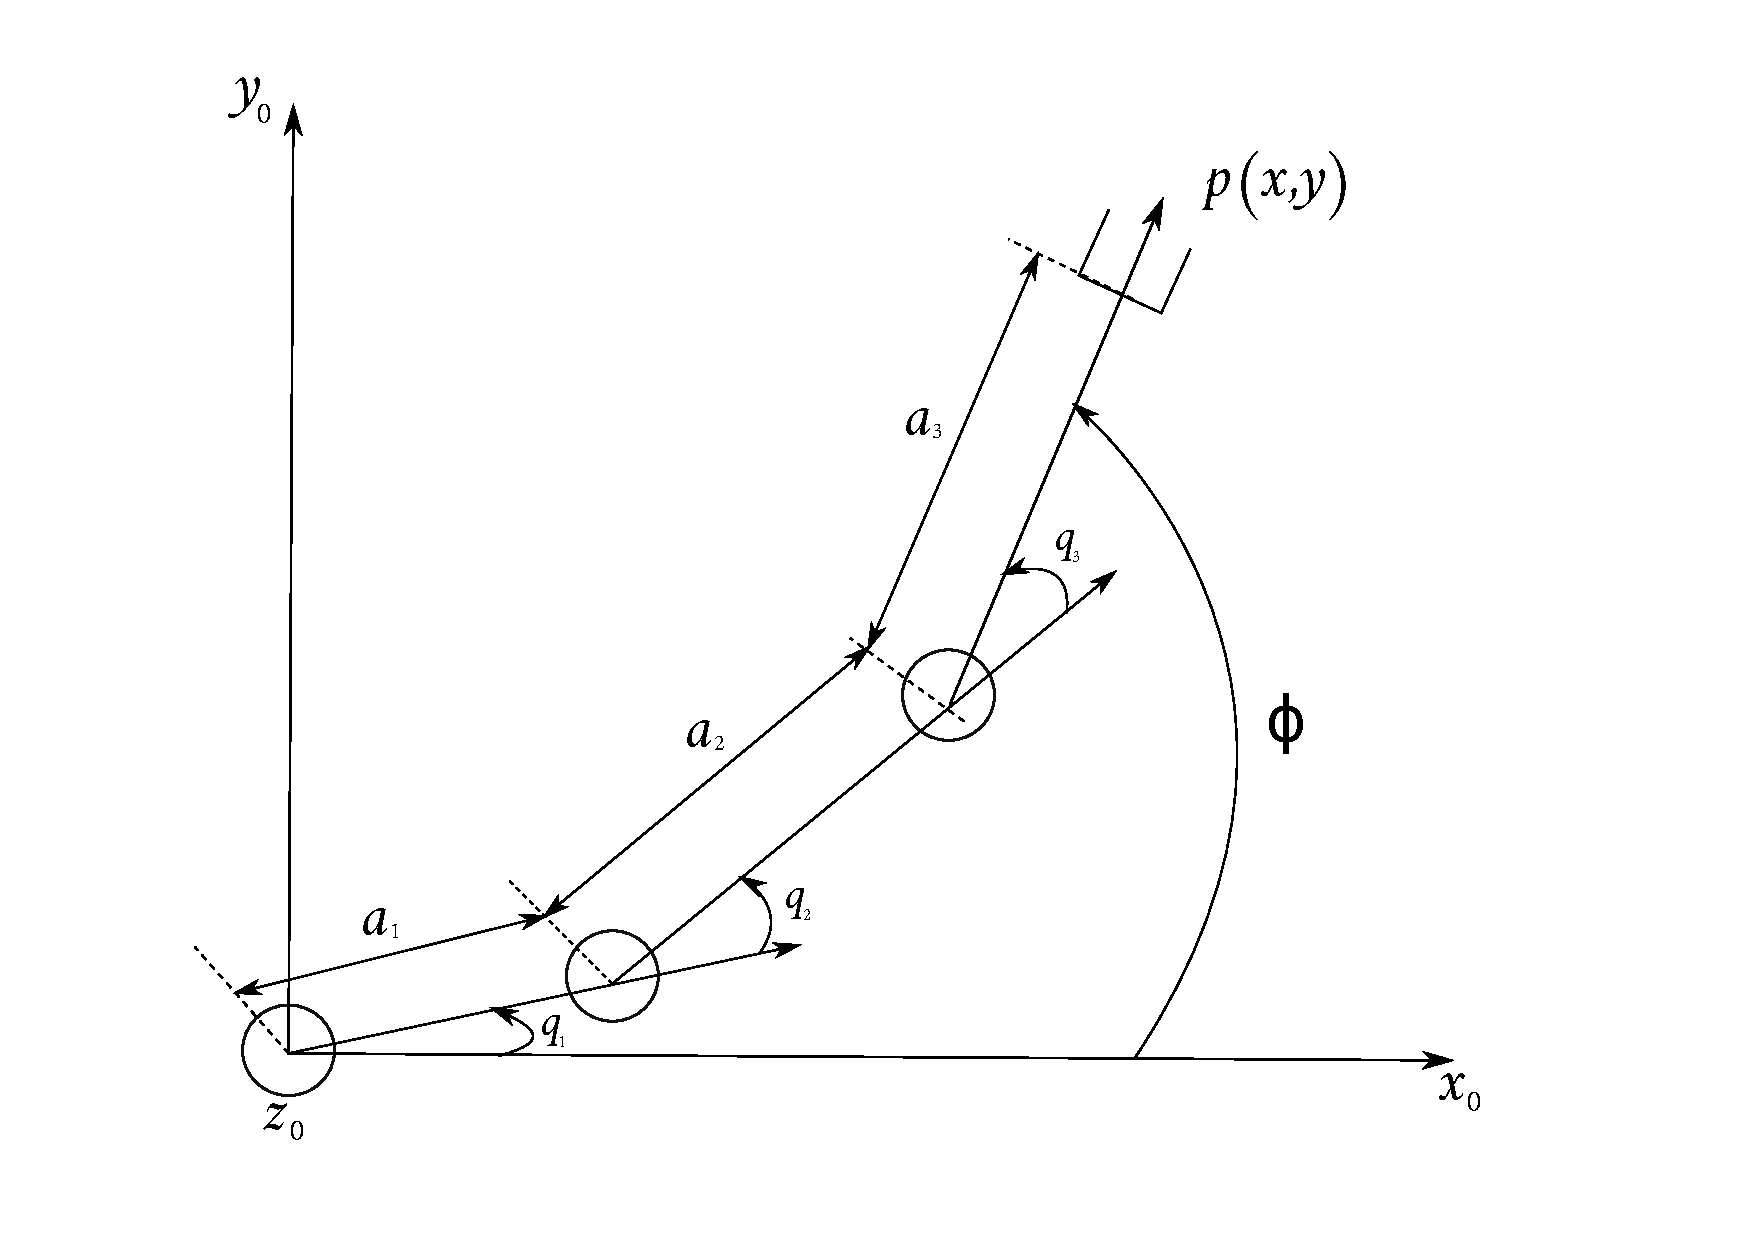
\includegraphics[scale=0.3]{manipolatore3RDiff.pdf}
\end{center}

\begin{equation}
	\underline{x} = \underline{f}(\underline{q}) \,=\,
	\begin{cases}
		x = a_1\,C_1 + a_2\,C_{12} + a_3\,C_{123} \\
		y = a_1\,S_1 + a_2\,S_{12} + a_3\,S_{123} \\
		\phi = q_1 + q_2 + q_3 \\
	\end{cases}
\end{equation}

a questo punto, deriviamo:
\begin{equation}
	\dot{\underline{x}} =   \frac{\partial \underline{f}(\underline{q})}{\partial \underline{q}} \cdot \underline{\dot{q}} = 
	\begin{cases}
		\dot{x} = \frac{\partial x}{\partial q_1} \dot{q_1} + \frac{\partial x}{\partial q_2} \dot{q_2} + \frac{\partial x}{\partial q_3} \dot{q_3} \\
		\dot{y} = \frac{\partial y}{\partial q_1} \dot{q_1} + \frac{\partial y}{\partial q_2} \dot{q_2} + \frac{\partial y}{\partial q_3} \dot{q_3} \\
		\dot{\phi} = \frac{\partial \phi}{\partial q_1} \dot{q_1} + \frac{\partial \phi}{\partial q_2} \dot{q_2} + \frac{\partial \phi}{\partial q_3} \dot{q_3} \\
	\end{cases}
\end{equation}

ovvero:
\begin{equation}
	\begin{bmatrix}
		\dot{x} \\
		\dot{y} \\
		\dot{\phi} \\
	\end{bmatrix}
	= 
	\begin{bmatrix}
		\frac{\partial x}{\partial q_1} & \frac{\partial x}{\partial q_2} & \frac{\partial x}{\partial q_3} \\
		\frac{\partial y}{\partial q_1} & \frac{\partial y}{\partial q_2} & \frac{\partial y}{\partial q_3} \\
		\frac{\partial \phi}{\partial q_1} & \frac{\partial \phi}{\partial q_2} & \frac{\partial \phi}{\partial q_3}
	\end{bmatrix}
	\cdot
	\begin{bmatrix}
		\dot{q_1} \\
		\dot{q_2} \\
		\dot{q_3} \\
	\end{bmatrix}
	\,\Rightarrow\,
	\begin{bmatrix}
		\dot{x} \\
		\dot{y} \\
		\dot{\phi} \\
	\end{bmatrix}
	= 
	J_a(q_1, q_2, q_3) \cdot
	\begin{bmatrix}
		\dot{q_1} \\
		\dot{q_2} \\
		\dot{q_3} \\
	\end{bmatrix}
\end{equation}

e pertanto, $J_a(\underline{q})$ risulta essere:
\begin{equation*}
	J_a(q_1, q_2, q_3) = 
	\begin{bmatrix}
		-(a_1\,S_1 + a_2\,S_{12} + a_3\,S_{123}) & -(a_2\,S_{12} + a_3\,S_{123}) & -a_3\,S_{123} \\
		a_1\,C_1 + a_2\,C_{12} + a_3\,C_{123} & a_2\,C_{12} + a_3\,C_{123} & a_3\,C_{123} \\
		1 & 1 & 1 \\
	\end{bmatrix}
\end{equation*}

\section{Jacobiano Geometrico}
La ($4.3$) ci fornisce una rappresentazione della \emph{velocità della terna utensile}, ma un'altra possibile descrizione è la seguente:
\begin{equation}
	\underline{v} = 
	\begin{bmatrix}
		\dot{\underline{p}} \\
		\underline{\omega} \\
	\end{bmatrix}
\end{equation}

dove $\dot{\underline{p}}$ indica la velocità di traslazione dell'origine della terna utensile rispetto alla terna base, mentre $\underline{\omega}$ è la velocità angolare della terna utensile, anch'essa relativamente alla terna base. Questa rappresentazione viene denominata \emph{screw di velocità}.

\paragraph{}
Con un ragionamento simile a quello di prima giungiamo alla seguente relazione matriciale:
\begin{equation}
	\underline{v} = J(\underline{q}) \cdot \dot{\underline{q}}
\end{equation}

definiamo $J(\underline{q}) \in \mathbb{R}^{6\times n}$ \emph{Jacobiano Geometrico} e mette in relazione lineare $\dot{\underline{q}}$ con $\underline{v}$. 

\paragraph{}
Otteniamo: 
\begin{equation}
	\underline{v} = 
	\begin{bmatrix}
		\underline{\dot{p}} \\
		\underline{\omega} \\
	\end{bmatrix}
	= J(\underline{q})\,\dot{\underline{q}} =
	\begin{bmatrix}
		J_p \\
		J_o \\
	\end{bmatrix}
	\cdot\underline{\dot{q}}
\end{equation}

quindi anche lo \emph{Jacobiano Geometrico} è composto da due sottomatrici $J_p \in\mathbb{R}^{3 \times n}$ e $J_o\in\mathbb{R}^{3 \times n}$ rispettivamente per la \emph{posizione} e per \emph{l'orientazione}.

pertanto:
\begin{equation}
	J = 
	\begin{bmatrix}
		J_p \\
		J_o \\
	\end{bmatrix}
	\, \Rightarrow \,
	\begin{cases}
		\underline{\dot{p}} = J_p \, \underline{\dot{q}} \\
		\underline{\omega} = J_o \, \underline{\dot{q}} \\
	\end{cases}
\end{equation}

\subsection{Calcolo di $J$}
Il calcolo dello Jacobiano geometrico $J$ si effettua considerando il contributo della velocità di ogni singolo giunto al moto dell'organo terminale, considerando tutti gli altri giunti bloccati, e sommando insieme tutti i contributi.

\paragraph{}
Ognuno dei contributi dei giunti al moto dell'organo terminale avrà un'espressione del tipo $\underline{J_i}\,\dot{q_i}$ dove $\underline{J_i}$ è la colonna \emph{i-esima} dello jacobiano. La velocità complessiva dell'organo terminale sarà quindi data da:

\begin{equation}
	\underline{v} = \sum_{i = 1}^{n} \underline{J_i}\,\dot{q_i} = 
	\begin{bmatrix}
		\,\underline{J_1} & \underline{J_2} & \cdots & \underline{J_n}\,
	\end{bmatrix}
	\begin{bmatrix}
		\dot{q_1} \\
		\dot{q_2} \\
		\vdots \\
		\dot{q_n}\\
	\end{bmatrix}
\end{equation}

per calcolare le colonne dello jacobiano, calcoliamo i vari contributi $\underline{J_i}\,\dot{q_i}$ distinguendo due casi: giunto $q_i$ \emph{rotoidale} e giunto $q_i$ \emph{prismatico}.

\subsubsection{Giunto Rotoidale}
Supponendo che il giunto \emph{i-esimo} sia rotoidale, una rotazione del giunto con velocità angolare $\dot{q_i}$, con tutti gli altri giunti bloccati, causerà una rotazione rigida della parte del robot che sta a valle del giunto $i$ attorno all'asse $z_{i-1}$ con velocità angolare espressa dal vettore: 
\begin{equation}
	\dot{q_i}\,\underline{k}_{i-1} 
\end{equation}
dove $\underline{k}_{i-1}$ è il versore del giunto $i$. Questo moto di rotazione attorno all'asse $z_{i-1}$ produce:
\begin{itemize}
	\item una velocità angolare dell'organo terminale, ovvero, del \emph{link n} pari a $\dot{q_i}\,\underline{k}_{\,i-1}$
	\item una velocità di traslazione del punto $\underline{p}$ pari a $\dot{q_i}\,\underline{k}_{\,i-1} \times (\,\underline{p} - \underline{O}_{\,i-1})$, dove $\underline{O}_{\,i-1}$ è il vettore posizione dell'origine della terna solidale al \emph{link i-1}
\end{itemize}

\begin{center}
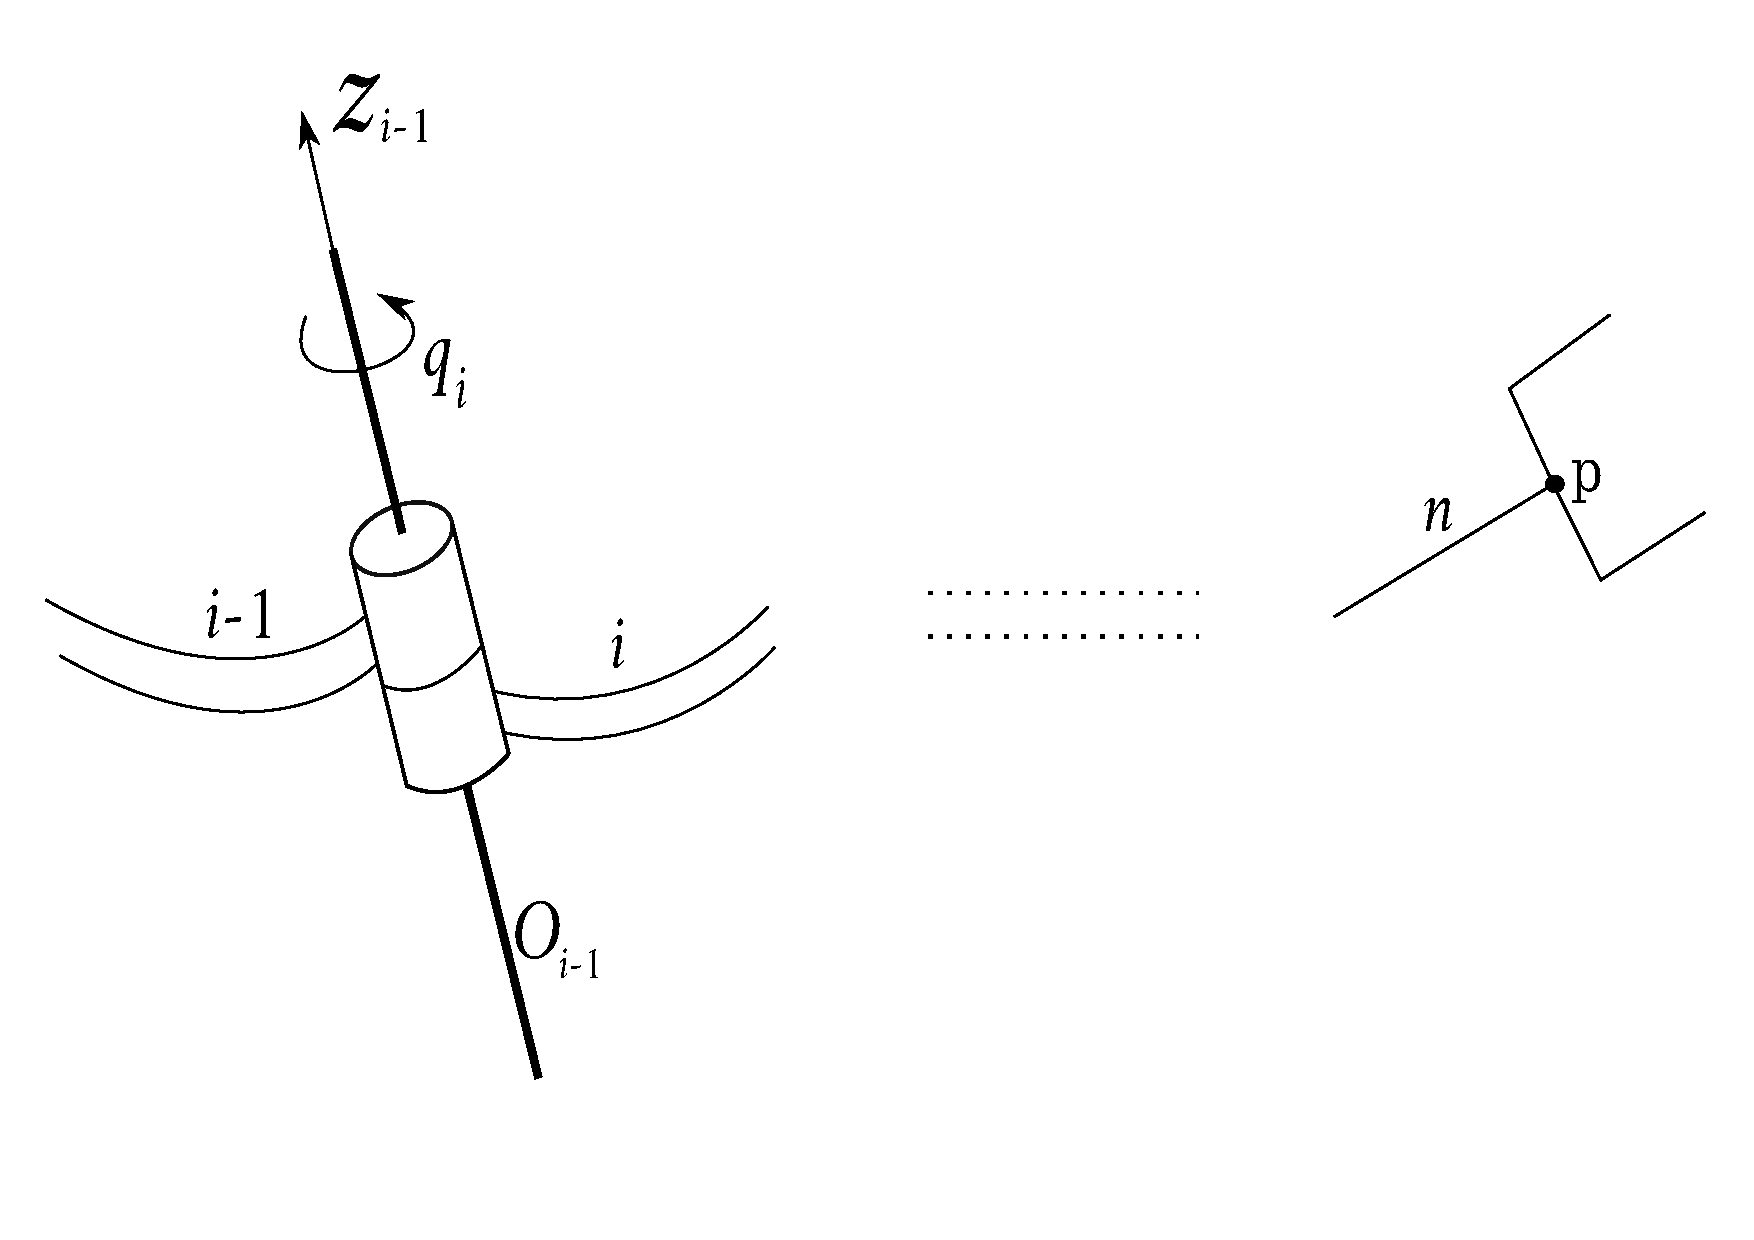
\includegraphics[scale=0.2]{giuntoRotoidale.pdf}
\captionof{figure}{Giunto rotoidale, i puntini indicano gli svariati giunti.}
\end{center}

\paragraph{}
Pertanto la colonna $\underline{J_i}$ dello jacobiano relativa al giunto $i$ risulta:
\begin{equation} \label{J_rotoidale}
	\underline{J}_{\,i} = 
	\begin{bmatrix}
		\underline{J}_{\,pi} \\
		\underline{J}_{\,oi} \\
	\end{bmatrix}
	= 
	\begin{bmatrix}
		\underline{k}_{\,i-1} \times (\,\underline{p} - \underline{O}_{\,i-1}) \\
		\underline{k}_{\,i-1}
	\end{bmatrix}
\end{equation}

\subsubsection{Giunto Prismatico}
Supponendo che il giunto \emph{i-esimo} sia prismatico, una traslazione del giunto con velocità $\dot{q_i}$, con tutti gli altri giunti bloccati, causerà una traslazione rigida della parte del robot che sta a valle del giunto $i$ lungo la direzione dell'asse $z_{i-1}$, con velocità angolare espressa dal vettore:
\begin{equation}
	\dot{d_i}\underline{k}_{\,i-1}
\end{equation}
dove $\underline{k}_{\,i-1}$ è il versore del giunto $i$. Tale moto di traslazione parallelo all'asse $z_{\,i-1}$ si traduce in:
\begin{itemize}
	\item un contributo nullo alla velocità angolare dell'organo terminale, ovvero del \emph{link n}
	\item un contributo alla velocità di traslazione del punto $\underline{p}$ pari a $\dot{d_i}\,\underline{k}_{\,i-1}$
\end{itemize}

\begin{center}
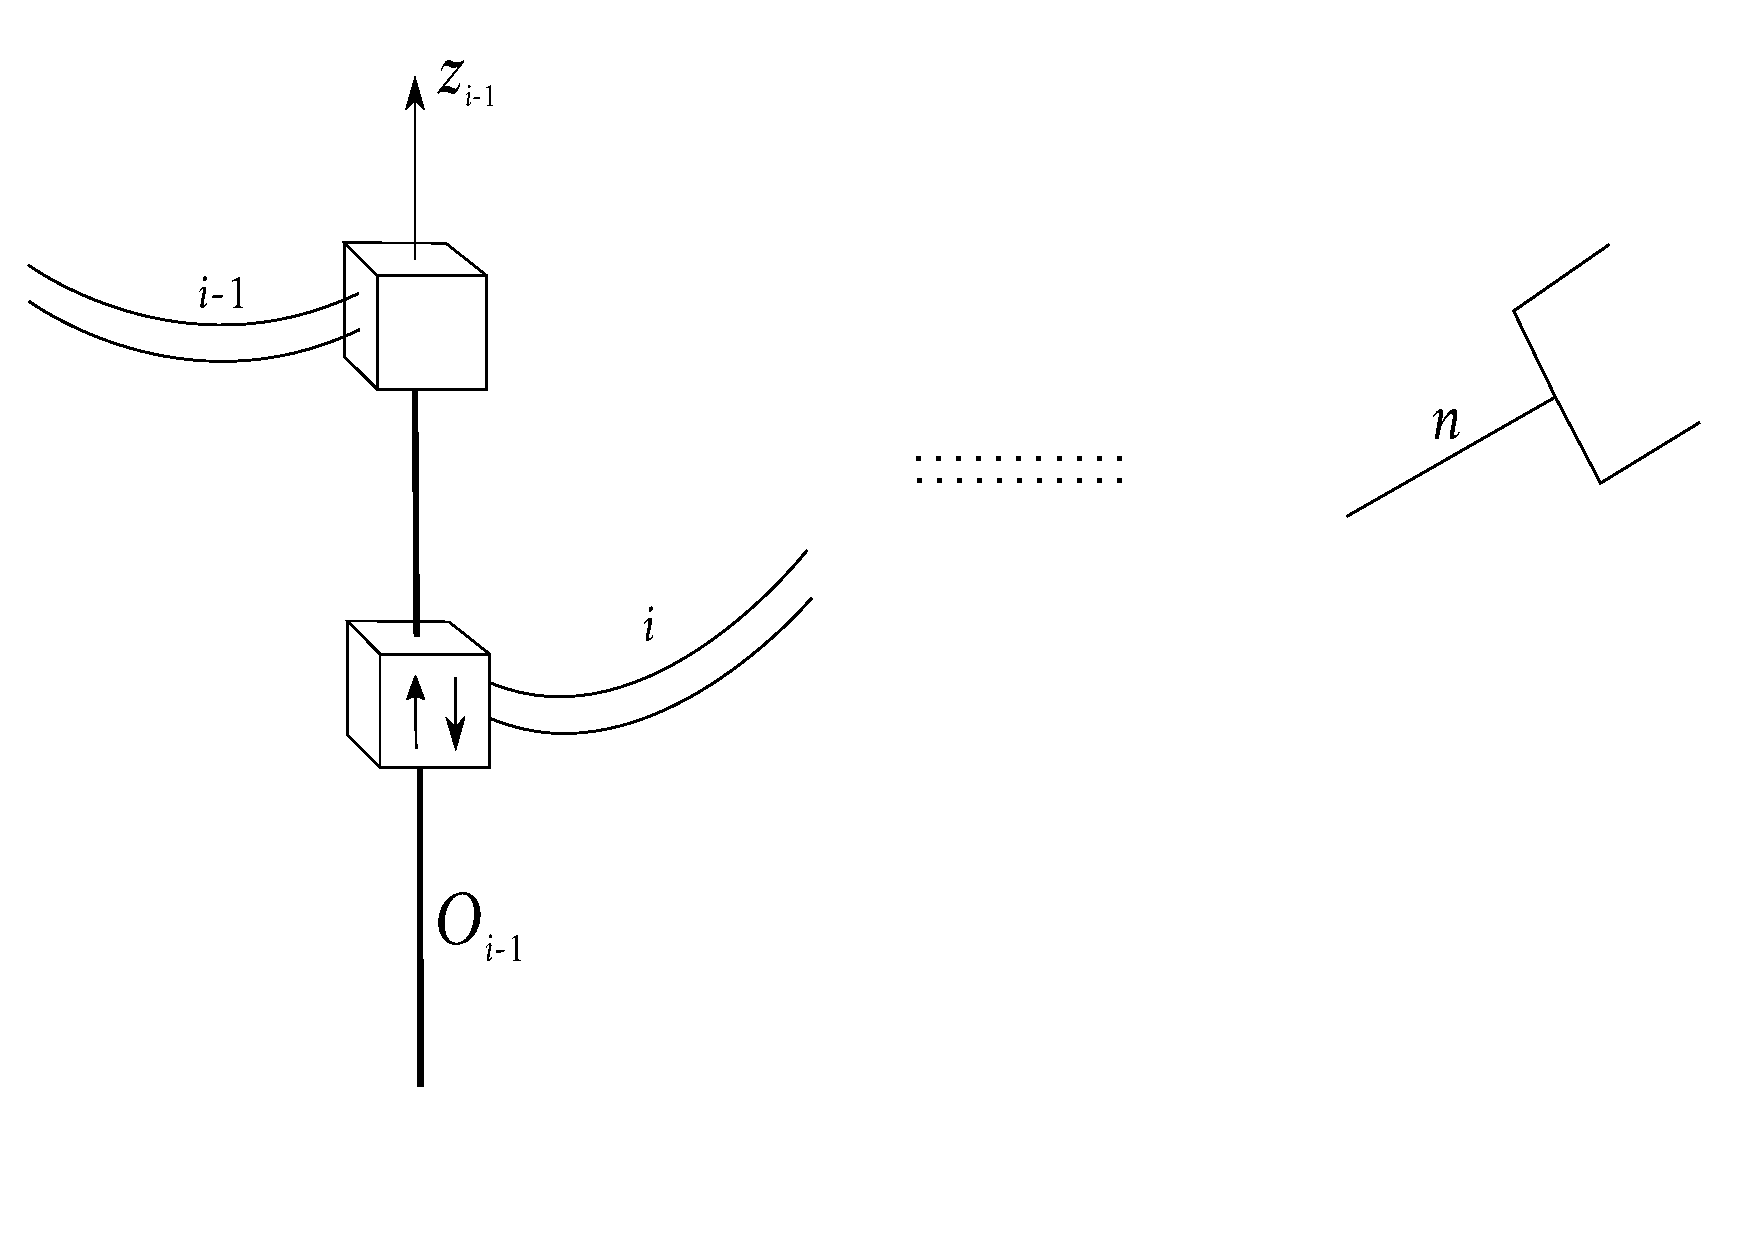
\includegraphics[scale=0.2]{giuntoPrismatico.pdf}
\captionof{figure}{Giunto prismatico, i puntini indicano gli svariati giunti.}
\end{center}

\paragraph{}
Pertanto la colonna $J_i$ dello jacobiano relativa al giunto $i$ risulta:
\begin{equation} \label{J_prismatico}
	\underline{J}_{\,i} = 
	\begin{bmatrix}
		\underline{J}_{\,pi} \\
		\underline{J}_{\,oi} \\
	\end{bmatrix}
	= 
	\begin{bmatrix}
		\underline{k}_{\,i-1} \\
		0 \\
	\end{bmatrix}
\end{equation}

\section{Relazione tra $J_a$ e $J$}
Esaminando la \eqref{J_rotoidale} e la \eqref{J_prismatico} notiamo che in generale vale $J_a \neq J$, ovvero, lo Jacobiano analitico è diverso dallo Jacobiano geometrico. Ma notiamo anche:
\begin{itemize}
	\item le parti traslazionali dei due Jacobiani coincidono: $J_{ap} = J_p$
	\item le parti rotazionali dei due Jacobiani differiscono: $J_{ao} \neq J_o$, perché $\underline{\omega} \neq \underline{\dot{\phi}}$
\end{itemize}

\paragraph{}
Cerchiamo il legame esistente tra $J_{ao}$ e $J_o$ nel caso in cui la rappresentazione dell'orientazione utilizzata sia quella di \emph{Eulero} $ZYZ$. Determiniamo il legame tra la velocità angolare di un corpo rigido e le derivate temporali degli angoli di Eulero che ne descrivono l'orientazione. Sfruttiamo il fatto che se ho $n+1$ corpi rigidi in moto ognuno rispetto al precedente allora:
\begin{equation} \label{omega}
	^0\underline{\omega}_{\,n,0} = \,^0\underline{\omega}_{\,1,0} + \,^0\underline{\omega}_{\,2,1} + \cdots + \,^0\underline{\omega}_{\,n,n-1}
\end{equation}

dove $^0\underline{\omega}_{\,i,i-1}$ è la \emph{velocità angolare} della terna $\langle i \rangle$ rispetto alla terna $\langle i-1 \rangle$ espressa in terna $\langle 0 \rangle$.

\paragraph{}
Esaminando le 4 terne di Eulero e le loro tre rotazioni:

\begin{center}
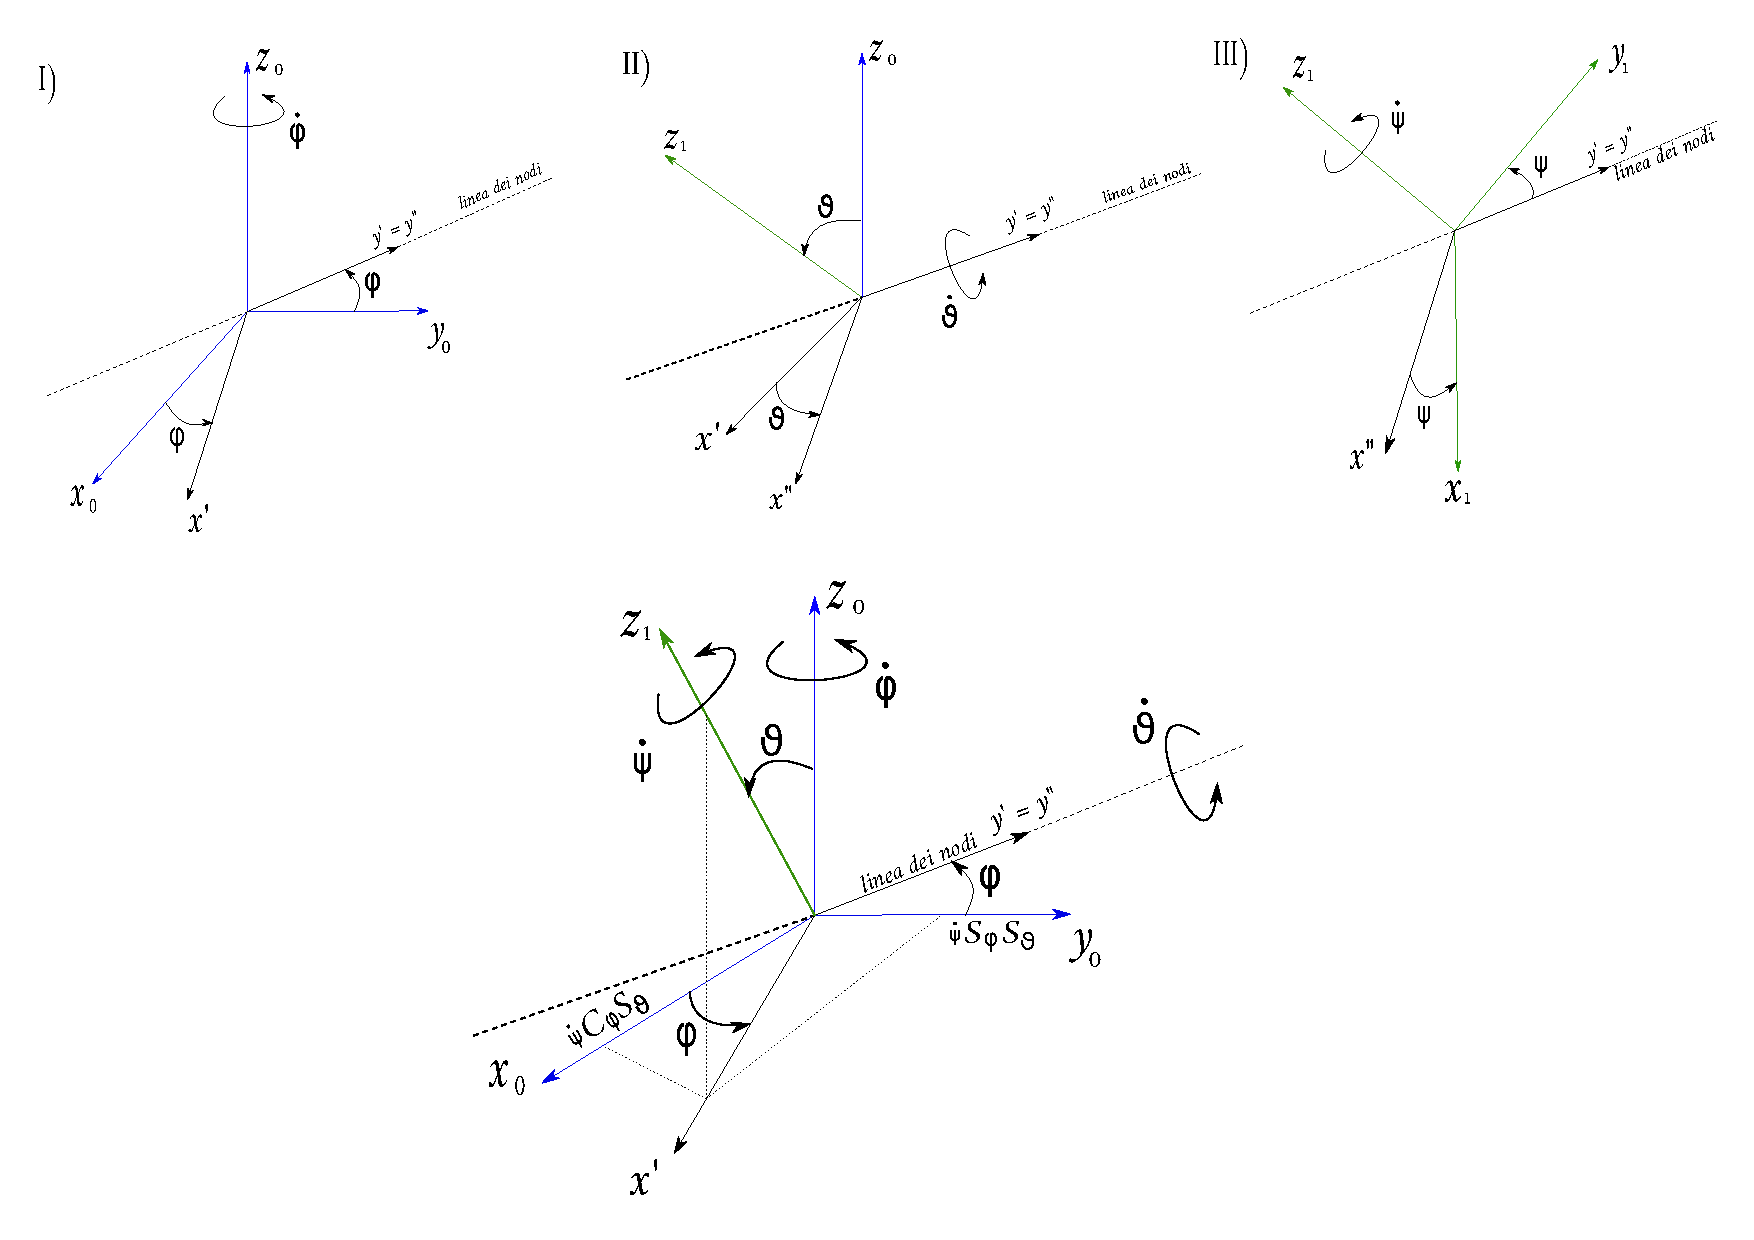
\includegraphics[scale=0.35]{rotazioniEuleroDiff.pdf}
\captionof{figure}{Le tre rotazioni di Eulero}
\end{center}

otteniamo:
\begin{equation*}
I)\;\;\dot{\varphi}\,\underline{k}_{\,0} = \dot{\varphi}
\begin{bmatrix}
	0 \\
	0 \\
	1 \\
\end{bmatrix}
\qquad
II)\;\;\dot{\theta}\,\underline{j}' = \dot{\theta}
\begin{bmatrix}
	- S_{\varphi} \\
	C_{\varphi} \\
	0 \\
\end{bmatrix}
\qquad
III)\;\;\dot{\psi}\underline{k}_{\,1} = 
\dot{\psi}
\begin{bmatrix}
	S_{\theta}C_{\varphi} \\
	S_{\theta}S_{\varphi} \\
	C_{\theta} \\
\end{bmatrix}
\end{equation*}

dove con $I)$, $II)$ e $III)$ indico le tre rotazioni.
\paragraph{}
Per quanto detto prima \eqref{omega}, possiamo esprimere la velocità angolare dell'ultima terna rispetto alla prima come la somma delle velocità angolari relativa di ogni terna rispetto alla precedente:
\begin{equation}
	\underline{\omega}=\dot{\varphi}\,\underline{k}_{\,0} + \dot{\theta}\,\underline{j}' + \dot{\psi}\underline{k}_{\,1} = 
	\begin{bmatrix}
		\underline{k}_{\,0} & \underline{j}' & \underline{k}_{\,1}
	\end{bmatrix}
	\begin{bmatrix}
		\dot{\varphi} \\
		\dot{\theta} \\
		\dot{\psi} \\
	\end{bmatrix}
\end{equation}

otteniamo:
\begin{equation}
	\underline{\omega} = T(\underline{\phi}) \cdot \dot{\underline{\phi}} \quad \text{con} \quad T(\underline{\phi}) = 
	\begin{bmatrix}
		\underline{k}_{\,0} & \underline{j}' & \underline{k}_{\,1} 
	\end{bmatrix}
	\quad \text{e} \quad \dot{\underline{\phi}} = 
	\begin{bmatrix}
		\dot{\varphi} \\
		\dot{\theta} \\
		\dot{\psi} \\
	\end{bmatrix}
\end{equation}

pertanto:
\begin{equation}
	T(\underline{\phi}) = 
	\begin{bmatrix}
		\underline{k}_{\,0} & \underline{j}' & \underline{k}_{\,1} 
	\end{bmatrix} = 
	\begin{bmatrix}
		0 & -S_{\varphi} & S_{\theta}C_{\varphi} \\
		0 & C_{\varphi} & S_{\theta}C_{\varphi} \\
		1 & 0 & C_{\theta} \\
	\end{bmatrix}
\end{equation}
\paragraph{}
Notiamo:
\begin{itemize}
	\item se siamo in \emph{singolarità di rappresentazione}, ovvero, $S_{\theta} = 0$ allora\\ 
	$det(T(\underline{\phi})) = 0$ e quindi $T(\underline{\phi})$ non è invertibile.
	\item se invece $det(T(\underline{\phi})) \neq 0$ allora la ($4.22$) può essere invertita: \begin{equation}
		\underline{\dot{\phi}} = T(\underline{\phi})^{-1} \cdot \underline{\omega}
	\end{equation}
\end{itemize}
\subsection{Calcolo di $J$ partendo da $J_a$ e viceversa}
Adesso consideriamo l'espressione di $\underline{\dot{\phi}}$ della ($4.6$) e andiamola a sostituire nella ($4.22$), otteniamo, considerando l'espressione di $\underline{\omega}$ della ($4.14$), due forme della $\underline{\omega}$ che possiamo eguagliare ottenendo:
\begin{equation}
	\begin{cases}
		\underline{\dot{\phi}} = J_{ao}\,\underline{\dot{q}} \\
		\underline{\omega} = T(\underline{\phi})\underline{\dot{\phi}}
	\end{cases}
	\;\Rightarrow\; 
	\begin{cases}
		\underline{\omega} = T(\underline{\phi})\,J_{ao}\,\underline{\dot{q}}\\
		\underline{\omega} = J_o \, \underline{\dot{q}} 
	\end{cases}
	\;\Rightarrow\;\;
	J_o = T(\underline{\phi})\,J_{ao}
\end{equation}
Se non siamo in singolarità di rappresentazione e quindi $S_{\theta} \neq 0$, possiamo invertire la relazione ottenendo:
\begin{equation}
	J_{ao} = T(\underline{\phi})^{-1}\,J_o
\end{equation}
A questo punto considerando $J_p = J_{ap} = I_{3 \times 3}\,J_{ap} + 0_{3 \times 3}\,J_{ao}$, dove $0_{3 \times 3}$ è una matrice di zeri $3 \times 3$ possiamo scrivere:
\begin{equation}
	J = 
	\begin{bmatrix}
	J_p \\
	J_o \\
	\end{bmatrix}
	=
	\underbrace{ 
	\begin{bmatrix}
		I_{3 \times 3} & 0_{3 \times 3} \\
		0_{3 \times 3} & T(\underline{\phi}) \\
	\end{bmatrix}
	}_{T_a(\underline{\phi})}
	\begin{bmatrix}
		J_{ap} \\
		J_{ao} \\
	\end{bmatrix}
	= 
	T_a(\underline{\phi})\,J_a
\end{equation}

dove abbiamo definito la matrice $T_a(\underline{\phi})\in\mathbb{R}^{6 \times 6}$. 
\paragraph{}
Dato che $T(\underline{\phi})$ è invertibile ($S_{\theta} \neq 0$) allora anche $T_a(\underline{\phi})$ è invertibile, otteniamo quindi:
\begin{itemize}
	\item Calcolo di $J$ partendo da $J_a$, $\Rightarrow$ $J = T_a(\underline{\phi})\,J_a$
	\item Calcolo di $J_a$ partendo da $J$, $\Rightarrow$ $J_a = T_a(\underline{\phi})^{-1}\,J$ 
\end{itemize}

\section{Singolarità Cinematica}
Una \emph{Singolarità Cinematica}, da qui in avanti indicata con il termine \emph{singolarità} o \emph{"punto singolare"} è una configurazione in cui lo Jacobiano Geometrico $J$ (oppure $J_a$) perde rango. Per un manipolatore nello spazio a 6 DOF, il termine \emph{"full rank"} indica che lo Jacobiano ha rango 6. Chiaramente la \emph{"Singolarità Cinematica"} è diversa dalla \emph{"Singolarità di Rappresentazione"}. 
\paragraph{}
Classifichiamo le singolarità cinematiche:
\begin{itemize}
	\item \textbf{Singolarità di confine:} Si presentano nelle configurazioni in cui il manipolatore è completamente esteso o completamente ripiegato su se stesso. Non rappresentano un grosso inconveniente perché risultano visibili. Si chiamano \emph{di confine} perché sono ai confini del \emph{workspace}.
	\item \textbf{Singolarità interna:} Causate solitamente dall’allineamento di qualche asse di giunto. Sono un problema perchè possono interessare traiettorie di lavoro del manipolatore. Si chiamano così \emph{interne} perché sono dentro il \emph{workspace}.
\end{itemize}
\paragraph{}
In corrispondenza delle \emph{singolarità} si verificano le seguenti circostanze di notevole interesse, perchè potenzialmente pericolose:
\begin{itemize}
	\item il manipolatore perde mobilità in certe direzioni
	\item possono esistere infinite soluzioni al problema cinematico
	\item in vicinanza delle singolarità, per far eseguire all'organo terminale piccoli \emph{screw di velocità} $\underline{v}$, i giunti del manipolatore devono muoversi con velocità molto elevate
\end{itemize} 

\subsection{Studio di singolarità}
Lo \emph{studio di singolarità} consiste nel cercare tutte le possibili configurazioni singolari di un dato manipolatore. Tale studio in generale non è facile e l'identificazione di tutte le singolarità di una data struttura di manipolazione non sempre è nota in forma chiusa. 
\paragraph{}
Un valore che ci è utile valutare per tale studio è \emph{l'indice di manipolabilità} $\sqrt{m}$ con $m = det(JJ^T)$, infatti, se $J$ perde rango, la matrice quadrata (e simmetrica) $JJ^T$ diventa singolare, ovvero con il determinante nullo.
\paragraph{}
Consideriamo $n$ il numero di gradi di libertà e supponiamo che il numero di variabili dello spazio operativo che servono per eseguire un determinato compito sia $r$, otteniamo:
\begin{equation}
	\underline{v} = J\,\underline{\dot{q}}, \quad \underline{\dot{q}}\in\mathbb{R}^n, \; \underline{v}\in\mathbb{R}^r
\end{equation}
Se $r<n$, il manipolatore risulta \emph{ridondante} da un punto di vista cinematico ed esistono $(n-r)$ gradi di libertà ridondanti. 

\paragraph{}
Lo Jacobiano caratterizza la trasformazione lineare dallo spazio delle velocità dei giunti allo spazio delle velocità dell'organo terminale. La trasformazione è illustrata in figura ($4.4$).
\begin{center}
\includegraphics[scale=0.35]{MappaturaCinDiff.pdf}
\captionof{figure}{Mappatura cinematica differenziale}
\end{center}
\paragraph{}
L'equazione cinematica differenziale ($4.28$) può essere caratterizzata in termini dell'\emph{immagine} e del \emph{nullo} della trasformazione, si ha che:
\begin{itemize}
	\item \emph{L'immagine} di J è il sottospazio $\mathcal{R}$(J) in $\mathbb{R}^r$ che individua le velocità dell'organo terminale che possono venir generate dalle velocità di giunto, nella configurazione assegnata al manipolatore.
	\item \emph{Il nullo} di J è il sottospazio $\mathcal{N}$(J) in $\mathbb{R}^n$ a cui appartengono le velocità di giunto che non producono alcuna velocità all'organo terminale, nella configurazione assegnata al manipolatore.
\end{itemize} 

\paragraph{}
Vale la seguente relazione:
\begin{equation}
	\text{dim}(\mathcal{R}(J)) + \text{dim}(\mathcal{N}(J)) = n
\end{equation}

Se lo Jacobiano è a \emph{rango pieno}, si ha: 
\begin{equation}
	\text{dim}(\mathcal{R}(J)) = r \qquad \text{dim}(\mathcal{N}(J)) = n-r
\end{equation}

Al contrario, se lo Jacobiano degenera in presenza di singolarità, la dimensione dell'\emph{immagine} diminuisce e allo stesso tempo aumenta quella del \emph{nullo}. Nei manipolatori ridondanti, si ha $\text{dim}(\mathcal{N}(J))>0$, essi prendono il nome di \emph{automoti}.

\subsubsection{Proiettori nel nullo di J}
Sia $P\in\mathbb{R}^{n \times n}$ si dice che è un \emph{proiettore} nel nullo di $J$ se: 
\begin{equation}
	\forall\underline{\dot{q}}\in\mathbb{R}^n \;\Rightarrow\; P\underline{\dot{q}}\in\mathcal{N}(J)
\end{equation}
supponiamo di avere una \emph{velocità desiderata} $\underline{v}_{\,des}$ e una $\underline{\dot{q}}$ tale da soddisfare 
\begin{equation}
	\underline{v}_{\,des} = J(\underline{q})\,\underline{\dot{q}}
\end{equation}
allora anche 
\begin{equation}
	\underline{\dot{q}} + P\,\underline{\dot{q}}_{\,a}
\end{equation}
con $\underline{\dot{q}}_{\,a}$ vettore arbitrario di \emph{velocità nello spazio dei giunti} è soluzione della ($4.32$), ovvero: 
\begin{equation}
	\underline{v}_{\,des} = J(\underline{\dot{q}} + P\,\underline{\dot{q}}_{\,a}) \qquad \forall \underline{\dot{q}}_{\,a}\in\mathbb{R}^n
\end{equation}

tale risultato è di importanza notevole per la risoluzione della ridondanza, poichè una soluzione del tipo ($4.33$) mette in luce la possibilità di scegliere il vettore $\underline{\dot{q}}_{\,a}$ in maniera tale da utilizzare vantaggiosamente i gradi di libertà ridondanti. In effetti, questo vettore arbitrario genera dei \emph{moti interni} della struttura che non apportano modifiche alla posa dell'organo terminale.

\subsection{Calcolo delle singolarità di struttura del manipolatore antropomorfo}
\paragraph{}
Esiste una classe di manipolatori a 6 DOF che semplifica il problema dello studio delle singolarità, si tratta di tutti i manipolatori dotati di \emph{polso sferico}. Per affrontare lo studio delle singolarità di un manipolatore con polso sferico e struttura portante (che può essere, ad esempio, antropomorfo, sferico o cilindrico), analizziamo lo Jacobiano geometrico $J$:

\begin{equation}
	J = 
	\begin{bmatrix}
		J_{1p} & J_{2p} & J_{3p} & J_{4p} & J_{5p} & J_{6p} \\
		J_{1o} & J_{3o} & J_{3o} & J_{4o} & J_{5o} & J_{6o} 
	\end{bmatrix}
	=
	\begin{bmatrix}
		J_{11} & J_{12} \\
		J_{21} & J_{22} \\
	\end{bmatrix}
	\quad \text{con} \quad J_{ij}\in\mathbb{R}^{3 \times 3}
\end{equation}
Se vogliamo $det(J_{12}) = \vert J_{12} \vert = 0$ oppure $\vert J_{21} \vert = 0$ allora:$\vert J \vert = \vert J_{11} \vert \cdot \vert J_{22} \vert$.
\paragraph{}
Per rendere nullo $\vert J_{12} \vert$, scegliamo di piazzare l’origine della terna utensile $\underline{O_6}$ nel \emph{centro del polso} $\underline{w}$, quindi otteniamo: $\vert J_{12} \vert = 0_{3 \times 3}$. Questo significa che possiamo studiare:
\begin{itemize}
	\item Gli zeri di $\vert J_{11} \vert$ (\emph{singolarità di struttura portante})
	\item Gli zeri di $\vert J_{22} \vert$ (\emph{singolarità di polso sferico})
\end{itemize}
procediamo con un esempio.
Calcoliamo le singolarità di struttura del manipolatore antropomorfo, per farlo, serviamoci della seguente figura:
\begin{center}
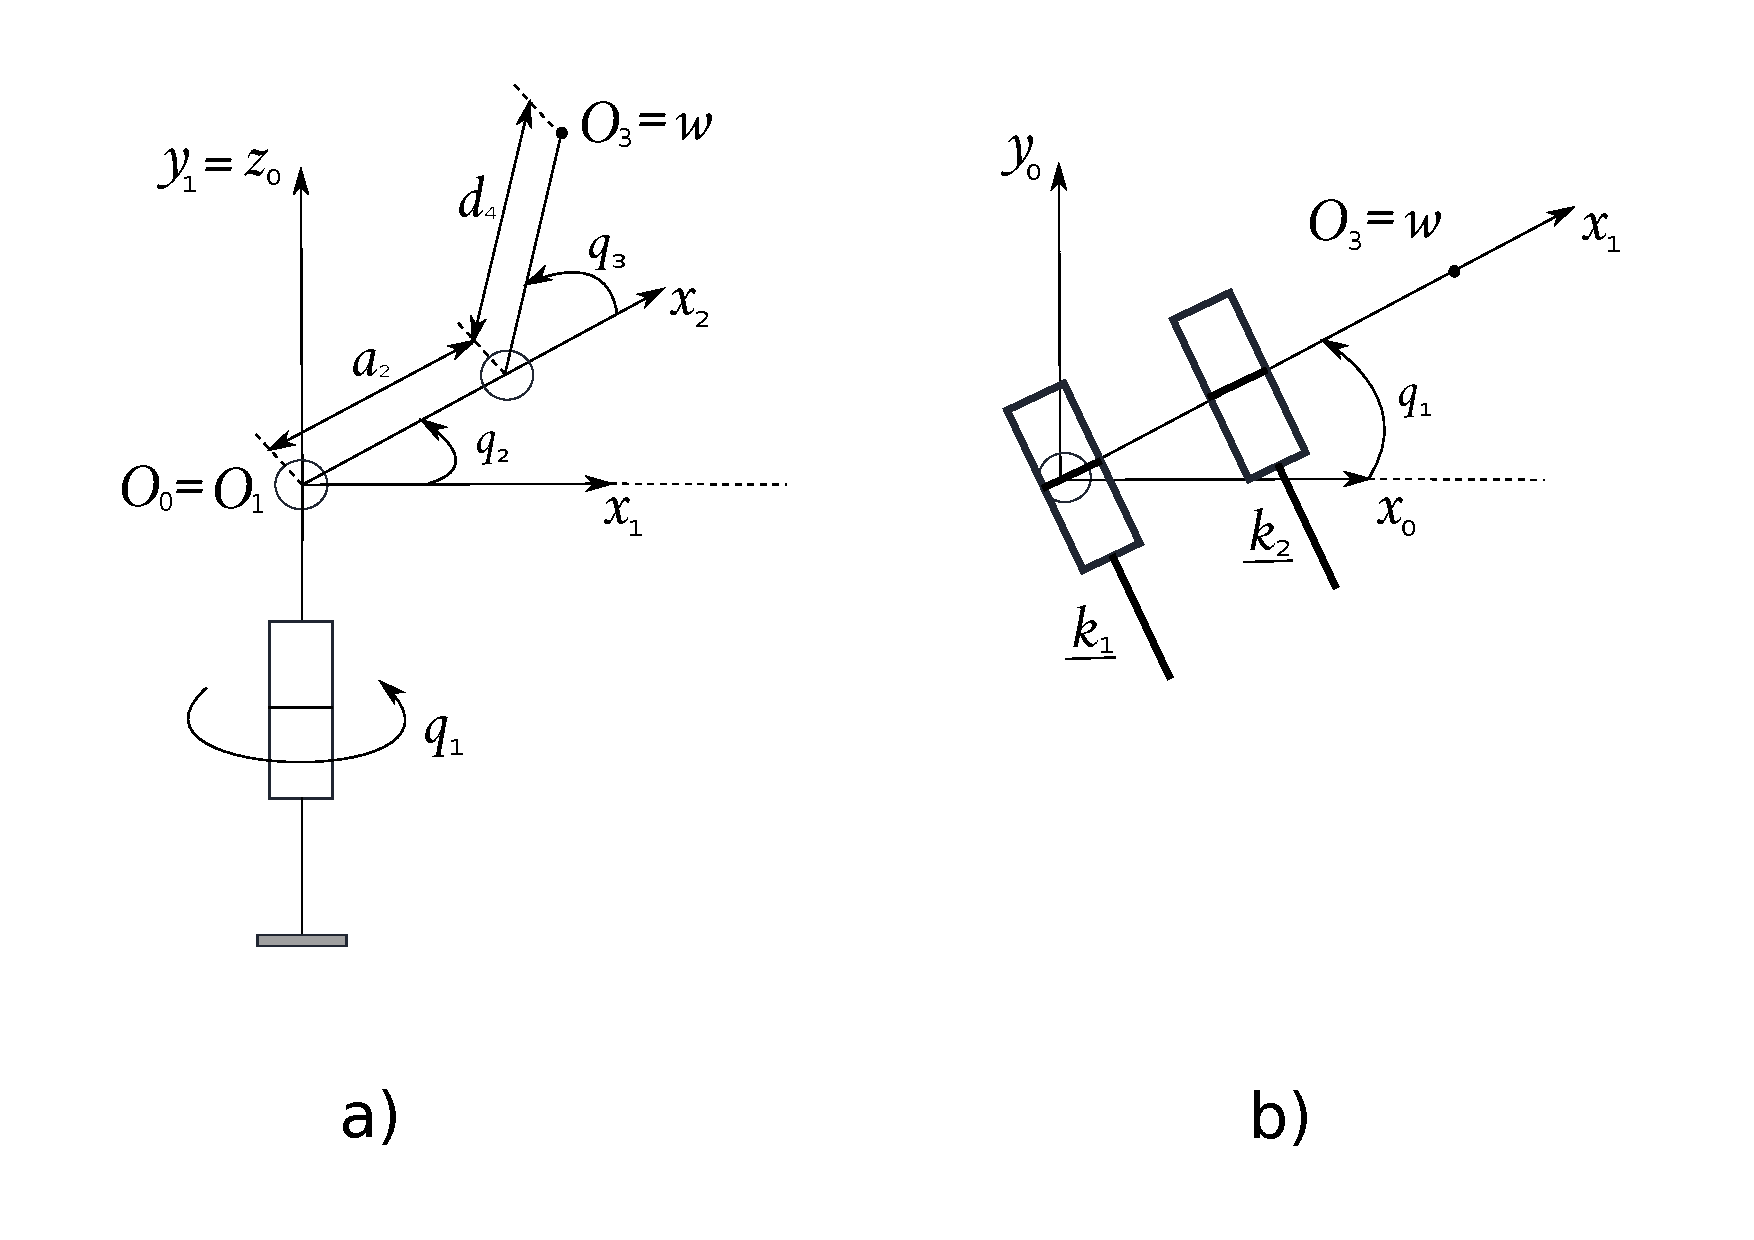
\includegraphics[scale=0.333]{visteManipolatoreDiff.pdf}
\captionof{figure}{vista in pianta: a) sul piano $x_1y_1$  b) sul piano $x_0y_0$}
\end{center}
Procediamo utilizzando due vie: quella geometrica e quella algebrica:

\subsubsection{Via Geometrica}
Si cerca di disegnare il manipolatore in configurazioni in cui una (o più) componenti di velocità di $w$ non sono realizzabili. Otteniamo:
\begin{itemize}
	\item si ha \emph{singolarità di gomito} quando $q_3 = 0$ (di confine)
	\item si ha \emph{singolarità di spalla} quando $w\in z_0\,\equiv\,y_1$ (interna), ovvero, quando $w_{x_1} = 0 = a_2C_2 + d_4C_{23} = 0$
\end{itemize}

esaminando il \emph{grado di mobilità} che si perde nei due casi:
\begin{itemize}
	\item Gomito: \emph{non} si può realizzare una velocità lungo $x_2$
	\item Spalla: \emph{non} si può realizzare una velocità in direzione $\perp$ al piano del braccio $x_1y_1$, cioè in direzione di $z_1 \parallel z_2$.
\end{itemize}

\subsubsection{Via Algebrica}
In linea generale, si cercano gli zeri di $J_{11}$. Iniziamo scrivendo $\underline{k_0}$, $\underline{k_1}$, $\underline{k_2}$:
\begin{equation}
	\underline{k_0} =
	\begin{bmatrix}
		0 & 0 & 1
	\end{bmatrix}^{T}
	\qquad \underline{k_1} =
	\begin{bmatrix}
		S_1 & -C_1 & 0
	\end{bmatrix}^{T}
	\qquad \underline{k_2} = \underline{k_1}
\end{equation}
adesso scriviamo $\underline{O_0}$, $\underline{O_1}$, $\underline{O_2}$, $\underline{O_3}$:
\begin{equation}
	\underline{O_0} = \underline{O_1} = 
	\begin{bmatrix}
		0 \\
		0 \\
		0 \\
	\end{bmatrix}
	\qquad \underline{O_2} =
	\begin{bmatrix}
		a_2C_1C_2 \\
		a_2S_1C_2 \\
		a_2S_2 \\
	\end{bmatrix}
	\qquad \underline{O_3} = w = 
	\begin{bmatrix}
		C_1(a_2C_2 + d_4C_{23}) \\
		S_1(a_2C_2 + d_4C_{23}) \\
		a_2S_2 + d_4S_{23} \\
	\end{bmatrix}
\end{equation}
possiamo scrivere adesso lo Jacobiano:
\begin{equation*}
	J_{11} = 
	\begin{bmatrix}
		\underline{k_0} \times (\underline{O_3} - \underline{O_0}) & \underline{k_1} \times (\underline{O_3} - \underline{O_1}) & \underline{k_2} \times (\underline{O_3} - \underline{O_2})
	\end{bmatrix}\in\mathbb{R}^{3 \times 3}
\end{equation*}

considerando che $\underline{O_0}$ e $\underline{O_1}$ sono nulli:
\begin{equation}
	J_{11} = 
	\begin{bmatrix}
		\underbrace{\underline{k_0} \times \underline{O_3}}_{\text{colonna 1}} & \underbrace{\underline{k_1} \times \underline{O_3}}_{\text{colonna 2}} & \underbrace{\underline{k_2} \times (\underline{O_3} - \underline{O_2})}_{\text{colonna 3}}
	\end{bmatrix}\in\mathbb{R}^{3 \times 3}
\end{equation}
\paragraph{}
Adesso andiamo a scrivere esplicitamente lo Jacobiano esprimendo il prodotto vettoriale con il formalismo matriciale introdotto a pagina $8$.
\begin{equation*}
	J_{11} = 
	\begin{bmatrix}
		\underbrace{
		\begin{bmatrix}
			0 & -1 & 0 \\
			1 & 0 & 0 \\
			0 & 0 & 0 \\
		\end{bmatrix}
		}_{S(\underline{k_0})}
		\underline{O_3} & 
		\underbrace{
		\begin{bmatrix}
			0 & 0 & -C_1 \\
			0 & 0 & -S_1 \\
			C_1 & S_1 & 0 \\
		\end{bmatrix}
		}_{S(\underline{k_1})}
		\underline{O_3} &
		\underbrace{
		\begin{bmatrix}
		0 & 0 & -C_1 \\
		0 & 0 & -S_1 \\
		C_1 & S_1 & 0 \\
		\end{bmatrix}
		}_{S(\underline{k_2})}
		(\underline{O_3} - \underline{O_2})
	\end{bmatrix}
\end{equation*}

considerando:
\begin{equation}
	(\underline{O_3} - \underline{O_2}) = 
	\begin{bmatrix}
		d_4C_1C_{23} \\
		d_4S_1C_{23} \\
		d_4S_{23} \\
	\end{bmatrix}
\end{equation}

a questo punto, svolgendo i prodotti matriciali considerando ($4.30$) e ($4.32$), otteniamo:
\begin{equation}
	J_{11} = 
	\begin{bmatrix}
		-S_1(a_2C_2 + d_4C_{23}) & -C_1(a_2S_2 + d_4S_{23}) & -C_1d_4S_{23} \\
		C_1(a_2C_2 + d_4C_23) & -S_1(a_2S_2 + d_4S_{23}) & -S_1d_4S_{23} \\
		0 & a_2C_2 + d_4C_{23} & d_4C_{23} \\
	\end{bmatrix}
\end{equation}
\paragraph{}
Calcoliamo il determinante $det(J_{11}) = \vert J_{11} \vert$ dello Jacobiano:
\begin{align*}
	\vert J_{11} \vert = -S_1(a_2C_2 + d_4C_{23})[-d_4S_1C_{23}(a_2S_2 + d_4S_{23}) + d_4S_1S_{23}(a_2C_2 + d_4C_{23})]- \\ 
	- C_1(a_2C_2 + d_4C_{23})[-d_4C_1C_{23}(a_2S_2 + d_4S_{23}) + d_4C_1S_{23}(a_2C_2 + d_4C_{23})] = \\
	= d_4S_1^2(a_2C_2 + d_4C_{23})[C_{23}(a_2S_2 + d_4S_{23}) - S_{23}(a_2C_2 + d_4C_{23})]+\\
	+ d_4C_1^2(a_2C_2 + d_4C_{23})[C_{23}(a_2S_2 + d_4S_{23}) - S_{23}(a_2C_2 + d_4C_{23})] = \\
	= d_4(a_2C_2 + d_4C_{23})[C_{23}(a_2S_2 + d_4S_{23}) - S_{23}(a_2C_2 + d_4C_{23})] = \\
	= d_4(a_2C_2 + d_4C_{23})[C_{23}a_2S_2 + C_{23}d_4S_{23} - a_2C_2S_{23} - d_4C_{23}S_{23}] = \\
	= d_4(a_2C_2 + d_4C_{23})[-a_2(S_{23}C_{2} - C_{23}S_2)] = \\
	= d_4(a_2C_2 + d_4C_{23})[-a_2\sin((q_2 + q_3) - q_2)] = \\
	= \underbrace{d_4(a_2C_2 + d_4C_{23})}_{\text{spalla}} \underbrace{[-a_2\sin(q_3)]}_{\text{gomito}}
\end{align*}\\\\\\


quindi otteniamo che il $\vert J \vert$ si annulla se:
\begin{itemize}
	\item $a_2C_2 + d_4C_{23} = 0$: il centro del polso si trova sull'asse del giunto 1, ovvero, sull'asse $z_0$. Il manipolatore perde mobilità nella direzione $z_1$. (\emph{singolarità di spalla})
	\item $S_3 = 0$: il link $2$ e $3$ sono allineati, il gomito è completamente steso ($q_3 = 0$) oppure completamente piegato ($q_3 = \pm\pi$). Il manipolatore perde mobilità nella direzione $x_2$. (\emph{singolarità di gomito})
\end{itemize}
\chapter{Inversione della cinematica differenziale}
\paragraph{}
L'equazione cinematica differenziale, rappresenta una trasformazione lineare tra \emph{spazio dei giunti} e \emph{spazio operativo}, infatti, essa stabilisce un legame lineare tra le \emph{velocità ai giunti} e la \emph{velocità dell'organo terminale} anche se è dipendente dalla \emph{configurazione del manipolatore}. Quindi, possiamo utilizzare l'equazione cinematica differenziale per affrontare il problema dell'inversione cinematica.  
\paragraph{}
Si supponga assegnata per l'organo terminale una \emph{traiettoria di moto} specificando $\underline{v}_{\,des}(t)$ e le condizioni iniziali su \emph{posizione e orientazione}. L'obiettivo è quello di determinare una possibile \emph{traiettoria ai giunti} $(\underline{q}(t), \underline{\dot{q}}(t))$ che riproduca la traiettoria data. Considerando la ($4.32$) nell'ipotesi $n = r$, ovvero, non vi sono manipolatori ridondanti e singolarità, otteniamo banalmente:
\begin{equation}
	\underline{\dot{q}} = J^{-1}(\underline{q})\,\underline{v}_{\,des}
\end{equation}
e chiaramente, conoscendo la postura iniziale del manipolatore $\underline{q}(0)$ possiamo calcolare la posizione $\underline{q}(t)$ integrando nel dominio del tempo. Questa integrazione si può effettuare al calcolatore tramite metodi numerici come quello di Eulero,
\begin{equation}
	\underline{q}(t) = \int_{t_i}^{t_f} \underline{\dot{q}}(t) dt \quad \Leftrightarrow \quad \underline{q}(t_{k+1}) = \underline{q}(t_k) + \underline{\dot{q}}(t_k)\Delta t 
\end{equation}

con l'istante $t_{k+1}$ scritto come: $t_{k+1} = t_k + \Delta t$. Quanto detto finora è valido solo se lo Jacobiano è a \emph{rango pieno}.

\section{Gestione della ridondanza}
Nel caso in cui si hanno delle ridondanze ($r<n$) e $J$ "obesa", un possibile metodo di soluzione è quello di formulare il problema della ricerca di soluzioni in termini di un problema di ottimo vincolato. Notiamo che $J$ potrebbe essere \emph{full rank}.
\paragraph{}
Una volta assegnata la velocità dell'organo terminale $\underline{v}_{\,des}$ e lo Jacobiano del manipolatore $J$ (per una data configurazione $\underline{q}$), si vogliono trovare le soluzioni $\underline{\dot{q}}$ che soddisfino l'equazione lineare ($4.32$) e che minimizzino il funzionale di costo quadratico delle velocità
\begin{equation}
	g(\underline{\dot{q}}) = \frac{1}{2}\underline{\dot{q}}^{T}W\underline{\dot{q}}
\end{equation}

dove $W\in\mathbb{R}^{n \times n}$ è una \emph{matrice di peso} simmetrica e definita positiva.\\
Il problema può essere risolto con il \emph{metodo dei moltiplicatori di Lagrange}, attraverso il \emph{funzionale di costo modificato},
\begin{equation}
	g(\underline{\dot{q}}, \underline{\lambda}) = \frac{1}{2}\underline{\dot{q}}^{T}W\underline{\dot{q}} + \lambda^T(\underline{v}_{\,des} - J\underline{\dot{q}})
\end{equation}

dove $\lambda \in\mathbb{R}^{r \times 1}$ è un vettore incognito di moltiplicatori che permette di incorporare il vincolo ($4.32$) nel funzionale da minimizzare, la soluzione cercata deve soddisfare le condizioni:
\begin{equation}
	\frac{\partial g}{\partial \underline{\dot{q}}} = 0 \qquad \frac{\partial g}{\partial \underline{\lambda}} = 0
\end{equation}
Otteniamo,
\begin{equation*}
	\begin{cases}
		\frac{\partial g}{\partial \underline{\dot{q}}} = \underline{\dot{q}}^TW - \underline{\lambda}^TJ = 0^T \\
		\frac{\partial g}{\partial \underline{\lambda}} = (\underline{v}_{\,des}- J\underline{\dot{q}})^T = 0^T
	\end{cases}
	\quad \Rightarrow \quad 
	\begin{cases}
		\underline{\dot{q}}^T = \underline{\lambda}^T JW^{-1} \\
		\underline{v}_{\,des} = J\underline{\dot{q}} 
	\end{cases}
	\quad \Rightarrow \quad
	\begin{cases}
		\underline{\dot{q}} = W^{-1}J^T \underline{\lambda} \\
		\underline{v}_{\,des} = JW^{-1}J^T \underline{\lambda}
	\end{cases}
\end{equation*}
Se $J$ è a rango pieno, anche $JW^{-1}J^T$ lo è, in quanto $W > 0$ e quindi ricaviamo 
\begin{equation}
	\underline{\lambda} = (JW^{-1}J^T)\underline{v}_{\,des}
\end{equation}

possiamo sostituirlo nell'espressione $\underline{\dot{q}} = W^{-1}J^T \underline{\lambda}$ e trovare $\underline{\dot{q}}$:
\begin{equation}
	\underline{\dot{q}} = \underbrace{W^{-1}J^T(JW^{-1}J^T)^{-1}}_{\text{pseudo-inversa pesata di J}}\,\underline{v}_{\,des}
\end{equation}

\paragraph{}
La matrice $W^{-1}J^T(JW^{-1}J^T)^{-1}$ è una \emph{inversa destra} di $J$, infatti, se premoltiplico per $J$ otteniamo
\begin{equation}
	J\Bigl[ W^{-1}J^T(JW^{-1}J^T)^{-1} \Bigr] = I_{r \times r}
\end{equation}

si può verificare infatti che la ($5.7$) soddisfa il vincolo di cinematica differenziale dato dalla ($4.32$) moltiplicando ambo i membri della ($5.7$) per $J$. Otteniamo infatti, $\underline{v}_{\,des} = J\,\underline{\dot{q}}$, ovvero, la ($4.32$).

\paragraph{}
Come sappiamo, la \emph{pseudo-inversa} esiste per ogni matrice, ma se scegliamo come \emph{matrice di peso} la matrice identità e $J$ è a \emph{rango pieno}, ricaviamo una particolare pseudo-inversa di $J$ detta \emph{pseudo-inversa di Moore Penrose},
\begin{equation}
	W = I_{r \times r} \quad \Rightarrow \quad \underline{\dot{q}} = \underbrace{ J^T(JJ^T)^{-1}}_{= J^{+}}\,\underline{v}_{\,des}
\end{equation}

è molto importante capire che se $J$ non ha rango pieno, $J^{+}$ non ha la forma scritta sopra. Notiamo che la $\underline{\dot{q}}$ trovata nella ($5.9$) minimizza la ($5.3$) e lo scarto $\| \underline{v}_{\,des} - J \underline{\dot{q}} \|$.
\newpage

\subsection{Soddisfacimento di vincoli aggiuntivi}
Ricordiamo, come detto nel paragrafo ($4.4.1$) che se $\underline{\dot{q}}^*$ soddisfa il vincolo $\underline{v}_{\,des} = J\underline{\dot{q}}^*$ e $P$ è un \emph{proiettore} su $\mathcal{N}(J)$, allora anche la seguente $\underline{\dot{q}}$ soddisfa il vincolo,
\begin{equation}
	\underline{\dot{q}} = \underline{\dot{q}}^* + P\underline{\dot{q}}_{\,a} \quad \textit{con $\underline{\dot{q}}_{\,a}$ arbitrario}
\end{equation}
\paragraph{}
Supponiamo di aver calcolato $\underline{\dot{q}}_{\,a}$ a partire da un criterio aggiuntivo che vogliamo soddisfare, formuliamo un problema di ottimizzazione con vincolo:
\begin{equation}
	g(\underline{\dot{q}}, \underline{\lambda}) = \frac{1}{2}(\underline{\dot{q}} - \underline{\dot{q}}_{\,a})^T \underbrace{I_{n \times n}}_{= W}(\underline{\dot{q}} - \underline{\dot{q}}_{\,a}) + \underline{\lambda}^T(\underline{v}_{\,des} - J\underline{\dot{q}})
\end{equation}

con tale scelta si vuole minimizzare la norma del vettore $\underline{\dot{q}} - \underline{\dot{q}}_{\,a}$, ovvero si cercano quelle soluzioni $\underline{\dot{q}}$ che soddisfino il vincolo cinematico ($4.32$) e che siano quanto più prossime a $\underline{\dot{q}}_{\,a}$. Procediamo,
\begin{equation*}
	\begin{cases}
		\frac{\partial g}{\partial \underline{\dot{q}}} = \underline{0}^T \\
		\frac{\partial g}{\partial \underline{\lambda}} = \underline{0}^T \\
	\end{cases}
	\quad \Rightarrow\quad
	\begin{cases}
		(\underline{\dot{q}}-\underline{\dot{q}}_{\,a})^T - \lambda^TJ = \underline{0}^T \\
		(\underline{v}_{\,des} - J\underline{\dot{q}})^T = \underline{0}^T
	\end{cases}
	\quad \Rightarrow \quad
	\begin{cases}
		\underline{\dot{q}} = \underline{\dot{q}}_{\,a} + J^T \underline{\lambda} \\
		\underline{v}_{\,des} = J \underline{\dot{q}}	
	\end{cases}
	\quad \Rightarrow
\end{equation*}
\begin{equation*}
	\Rightarrow \quad 
	\begin{cases}
		\underline{\dot{q}} = J^T \underline{\lambda} + \underline{\dot{q}}_{\,a} \\
		\underline{v}_{\,des} = JJ^T \underline{\lambda} + J \underline{\dot{q}}_{\,a}
	\end{cases}
	\quad \Rightarrow \quad
	\begin{cases}
		\underline{\dot{q}} = J^T \underline{\lambda} + \underline{\dot{q}}_{\,a} = J^T \underline{\lambda} + I\underline{\dot{q}}_{\,a} \\
		\underline{\lambda} = (JJ^T)^{-1} \underline{v}_{\,des} - (JJ^T)^{-1}J \underline{\dot{q}}_{a} 
	\end{cases}
\end{equation*}

possiamo fare questa operazione perchè essendo $J$ a rango pieno, allora esiste l'inversa di $JJ^T$. Scriviamo $\underline{\dot{q}}$ con $\underline{\lambda}$ esplicito:

\begin{eqnarray*}
	\underline{\dot{q}} = J^T \Bigl[ (JJ^T)^{-1}\underline{v}_{\,des} - (JJ^T)^{-1}J \underline{\dot{q}}_{\,a} \Bigr] + I \underline{\dot{q}}_{\,a} = \\
	= J^T (JJ^T)^{-1}\underline{v}_{\,des} + \underbrace{\Bigl[ I - J^T(JJ^T)^{-1}J \Bigr]}_{\boxdot} \underline{\dot{q}}_{\,a}
\end{eqnarray*}

dobbiamo verificare che $\boxdot$ sia un \emph{proiettore nel nullo} di $J$ per assicurarsi che $\boxdot\underline{\dot{q}}_{\,a}$ non modifichi il moto $\underline{v}_{\,des}$. Per verificarlo, moltiplichiamo per $J$,
\begin{equation}
	J\boxdot\underline{\dot{q}}_{\,a} = J\Bigl[ I - J^T(JJ^T)^{-1}J \Bigr]\underline{\dot{q}}_{\,a} = \Bigl[ J - \underbrace{JJ^T(JJ^T)^{-1}}_{I}J \Bigr] \underline{\dot{q}}_{\,a} = \underline{0}
\end{equation}

dopo aver verificato e ricordando che $J^{+} = J^T(JJ^T)^{-1}$, riscriviamo $\underline{\dot{q}}$ nel seguente modo:
\begin{equation}
	\underline{\dot{q}} = J^{+} \underline{v}_{\,des} + (I - J^{+}J) \underline{\dot{q}}_{\,a}
\end{equation}

La matrice ($I - J^{+}J$) è una delle possibili matrici $P$ della ($5.10$), che consente di proiettare $\underline{\dot{q}}_{\,a}$ nel nullo di $J$, così da non violare il vincolo cinematico dettato dalla ($4.32$), pertanto nel caso di $\underline{v}_{\,des} = 0$ è possibile generare dei \emph{moti interni} descritti da $(I-J^+J)\underline{\dot{q}}_{\,a}$ che riconfigurano il manipolatore lasciando inalterata la posa del suo organo terminale.

\subsection{Possibili applicazioni}
Dato che possiamo scegliere $\underline{\dot{q}}_{\,a}$, possiamo decidere le variabili di giunto e ottenere i seguenti risultati:
\begin{itemize}
	\item \emph{misura di manipolabilità}: possiamo gestire $\sqrt{m} = \sqrt{det\Bigl(J(\underline{q})J^{T}(\underline{q})\Bigr)}$ perchè sappiamo che si annulla in corrispondenza di una configurazione singolare, per cui massimizzando tale indice si utilizza la ridondanza per allontanarsi dalle singolarità. 
	\item \emph{distanza dai fine-corsa dei giunti}: attraverso una funzione obiettivo possiamo tenere sotto controllo la massima escursione ammessa per ogni variabile di giunto.
	\item \emph{distanza da un ostacolo}: possiamo gestire il minimo della norma tra la coordinata di giunto e la posizione dell'ostacolo gestita da un vettore.
\end{itemize}

\section{Gestione delle singolarità}
Fino adesso, l'inversione della cinematica differenziale è possibile attraverso le equazioni ($5.9$) e ($5.1$), ovvero:
\begin{equation}
	\underline{\dot{q}} = J^{-1}(\underline{q})\,\underline{v}_{\,des} \quad\qquad \underline{\dot{q}} = J^+\underline{v}_{\,des}
\end{equation}  
ma queste equazioni valgono solo se $J$ è a rango pieno. Esse, pertanto perdono di significato quando il manipolatore è in una \emph{configurazione singolare}, in tal caso il sistema $\underline{v}_{\,des} = J\underline{\dot{q}}$ contiene equazioni \emph{linearmente dipendenti}.
\paragraph{}
Distinguiamo due casi:
\begin{itemize}
	\item Si può determinare una soluzione in $\underline{\dot{q}}$ solo se $\underline{v}_{\,des}\in \mathcal{R}(J)$, estraendo tutte le equazioni linearmente dipendenti. Ovvero, il percorso assegnato nello spazio operativo è fisicamente eseguibile da parte del manipolatore anche se si trova in configurazione singolare.
	\item Se $\underline{v}_{\,des}\not\in \mathcal{R}(J)$ il sistema non è risolvibile, questo perchè il percorso assegnato nello spazio operativo non è eseguibile da parte del manipolatore nella postura assegnata.
\end{itemize}
Notiamo che l'inversione dello Jacobiano è un problema non solo in corrispondenza di un valore singolare ma anche nell'intorno di essa, infatti calcolando $J^{-1}$ dobbiamo calcolare il determinante di $J$, e questo è nullo in corrispondenza dei valori singolari e assume dei valori piccoli nell'intorno di una singolarità e questo da luogo a velocità elevate dei giunti.
\paragraph{}
Aggiriamo il problema di inversione nell'intorno di una singolarità attraverso l'uso di una \emph{pseudo-inversa smorzata}:
\begin{equation}
	J^* = J^T(JJ^T + K^2I)^{-1}
\end{equation}
dove $K$ è un \emph{fattore di smorzamento} che equivale ad un numero piccolo che viene posizionato lontano dalle singolarità e tende a crescere in prossimità di esse. Quindi $\underline{\dot{q}}$ non si ottiene più dalle equazioni in ($5.14$) ma:
\begin{equation}
	\underline{\dot{q}} = J^T(JJ^T + K^2I)^{-1} \,\underline{v}_{\,des}
\end{equation}

\section{Algoritmi di CLIK}
L'inversione cinematica è affidata ad una integrazione numerica vista nella ($5.2$), e la variabile di giunto $\underline{q}$ ad un certo istante è calcolata con l'inversa dello Jacobiano valutata nei giunti all'istante precedente,
\begin{equation}
	\underline{q}(t_{k+1}) = \underline{q}(t_k) + \underline{\dot{q}}(t_k)\Delta t = \underline{q}(t_k) + J^{-1}(\underline{q}(t_k))\,\underline{v}_{\,des}(t_k)\Delta t
\end{equation}
pertanto la ricostruzione della variabile di giunto ha dei fenomeni di deriva, quindi non si ottiene la posa dell'organo terminale desiderata.

Per risolvere questo problema ricorriamo a uno \emph{schema di soluzione} che tenga conto dell'errore nello spazio operativo tra la posa desiderata e quella calcolata,
\begin{equation}
	\underline{e} = \underline{x}_{\,des} - \underline{x}
\end{equation}
possiamo immaginare l'errore come in figura seguente:
\begin{center}
	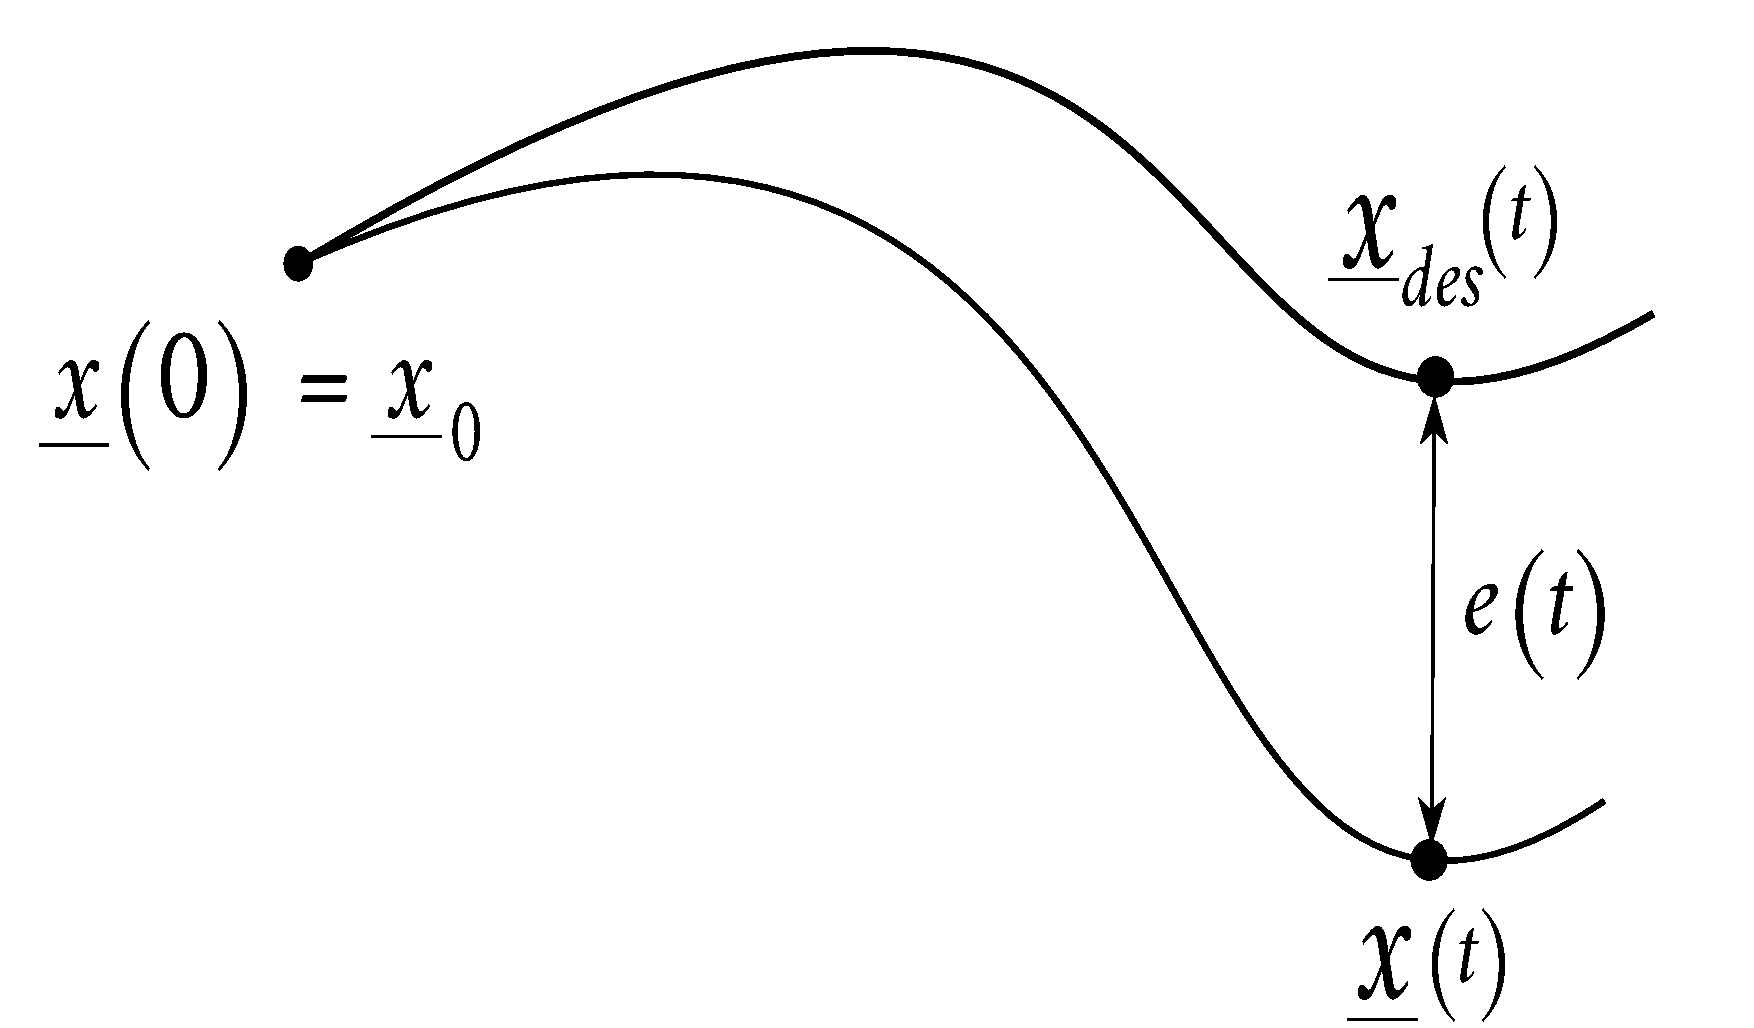
\includegraphics[scale=0.15]{errore.pdf}
\end{center}
Consideriamo la derivata temporale dell'errore che considerando la ($4.6$) otteniamo,
\begin{equation}
	\underline{\dot{e}} = \underline{\dot{x}}_{\,des} - \underline{\dot{x}} = \underline{\dot{x}}_{\,des} - J_a(\underline{q})\underline{\dot{q}}
\end{equation}
per far si che l'equazione ($5.19$) dia luogo ad un \emph{algoritmo per l'inversione cinematica}, servono due condizioni:
\begin{enumerate}
	\item La dipendenza tra $\underline{\dot{q}}$ ed $\underline{e}$ deve dare vita ad una equazione differenziale che caratterizzi l'evoluzione dell'errore nel tempo.
	\item La dipendenza tra $\underline{\dot{q}}$ ed $\underline{e}$ deve assicurare la convergenza a zero dell'errore.
\end{enumerate}
questa dipendenza da vita ai seguenti algoritmi \emph{closed loop inverse kinematic} (clik) per l'inversione cinematica. 

\subsection{Pseudo-inversa dello Jacobiano}
\paragraph{}
Ipotizziamo che la matrice $J_a$ quadrata sia \emph{non} singolare, possiamo scrivere $\underline{\dot{q}}$ in maniera algoritmica,
\begin{equation}
	\underline{\dot{q}} = J_a^{-1}(\underline{q})(\underline{\dot{x}}_{\,des} + K\underline{e})
\end{equation}
ottenendo 
\begin{equation}
	\underline{\dot{e}} + K\underline{e} = 0 \quad \Rightarrow \quad \underline{e}(t) = e^{-Kt}e_0,\;\; e_0 = 0
\end{equation}
se gli autovalori di $-K$ sono a parte reale negativa allora il sistema è globalmente e asintoticamente stabile. In effetti, la matrice $K$ è \emph{definita positiva} come scelta del progettista. 

Quindi l'errore tende a zero lungo la traiettoria con una velocità di convergenza che dipende dagli autovalori di $K$, più questi sono grandi, più veloce è la convergenza.

Lo schema a blocchi che realizza l'inversione cinematica secondo la ($5.20$) è rappresentato in Figura ($5.1$), 
\begin{center}
	\includegraphics[scale=0.35]{algInversaJacobiano.pdf}
	\caption{Schema a blocchi dell'algoritmo per l'inversione cinematica con $J_a^{-1}$}
\end{center}
analizziamolo:
\begin{itemize}
	\item Il blocco $K$ rappresenta un guadagno costante che rende il sistema asintoticamente stabile.
	\item Il blocco $kin(\cdot)$ rappresenta la funzione cinematica diretta, è un blocco non lineare ed è necessario al computo di $\underline{x}_{\,des}$ e anche al relativo errore di inseguimento.
	\item Il blocco $J_a^{-1}$ compensa $J_a$ e quindi fa si che il sistema sia lineare.
	\item Il blocco $\int$ nella catena diretta garantisce per un riferimento costante ($\underline{\dot{x}}_{\,des} = 0$) un errore a regime nullo.
	\item L'azione in \emph{feedforward} fornita da $\underline{\dot{x}}_{\,des}$ garantisce, in caso di riferimento non costante nel tempo, che l'errore si mantenga nullo lungo la traiettoria. Chiaramente, deve valere $\underline{e}(0) = 0$. 
\end{itemize}
\paragraph{}
Nel caso di un \emph{manipolatore ridondante}, la generalizzazione della ($5.20$) consente di ricavare una soluzione algoritmica del tipo,
\begin{equation}
	\underline{\dot{q}} = J^+_a(\underline{x}_{\,des} + K\underline{e}) + (I - J^+_aJ_a)\underline{\dot{q}}_{\,a}
\end{equation}
che corrisponde alla ($5.13$).

La struttura dell'algoritmo per l'inversione cinematica può essere concettualmente adottata ai fini di una tecnica di controllo semplice di un robot, nota sotto il nome di \emph{controllo cinematico}.

\subsection{Trasposta dello Jacobiano}
Un algoritmo di inversione cinematica più semplice di quello precedente dal punto di vista computazionale può essere ricavato dal legame tra $\underline{\dot{q}}$ ed $\underline{e}$ che assicuri la convergenza a zero dell'errore ma che non effettui la linearizzazione della ($5.19$). 

Quindi, la dinamica di errore è governata da un'equazione differenziale non lineare. Utilizziamo il \emph{metodo diretto di Lyapunov} per assicurarci la stabilità del sistema. I passi da seguire sono:
\begin{itemize}
	\item Definiamo una funzione candidata di Lyapunov $V(\underline{e})>0$ \emph{radially unbounded}.
	\item Cerchiamo $\underline{\dot{q}}$ in modo che $\dot{V}(\underline{e}) \leqslant 0$
\end{itemize}
\paragraph{}
Si scelga come funzione cadidata di Lyapunov la forma quadratica definita positiva
\begin{equation}
	V(\underline{e}) = \frac{1}{2}\underline{e}^TK\underline{e}
\end{equation} 
con $K$ matrice simmetrica e definita positiva. Tale funzione gode della seguente proprietà
\begin{equation}
	V(\underline{e})>0\quad \forall \underline{e} \neq \underline{0}, \quad V(\underline{0})= 0
\end{equation}
e pertanto differenziando la ($5.23$) rispetto al tempo e considerando la ($5.19$), si ha
\begin{equation}
	\dot{V}(\underline{e}) = \frac{\partial V}{\partial \underline{e}}\, \underline{\dot{e}} = \underline{e}^T K \underline{\dot{e}} = \underline{e}^TK \underline{\dot{x}}_{\,des} - \underline{e}^TK \underline{\dot{x}}
\end{equation}
A questo punto, scegliendo la velocità ai giunti come,
\begin{equation}
	\underline{\dot{q}} = J_a^TK\underline{e}
\end{equation}
otteniamo,
\begin{equation}
	\dot{V}(\underline{e}) = \underline{e}^TK \underline{\dot{x}}_{\,des} - \underline{e}^TK J_aJ_a^TK\underline{e}
\end{equation}
\paragraph{}
Si consideri il caso di riferimento costante, ovvero $\underline{\dot{x}}_{\,des} = \underline{0}$, otteniamo
\begin{equation}
	\dot{V}(\underline{e}) = - \underline{e}^TK J_aJ_a^TK\underline{e}
\end{equation}

notiamo che:
\begin{itemize}
	\item Se ipotizziamo che $J_a$ sia di rango pieno, la funzione ($5.28$) risulta \emph{definita negativa}.
	\item Se inoltre, imponiamo $\dot{V}<0$ e $V>0$ otteniamo $\underline{e} = \underline{0}$, ovvero, il sistema risulta \emph{asintoticamente stabile}.
	\item Se $\mathcal{N}(J_a^T) \neq 0$, la funzione ($5.28$) risulta \emph{semi-definita negativa}, infatti otteniamo che $\dot{V} = 0$ per $\underline{e} \neq \underline{0}$ e pertanto $K\underline{e} \in \mathcal{N}(J_a^T)$. In questo caso la ($5.28$) evidenzia che l'algoritmo si trova in \emph{stallo}, ovvero, $\underline{\dot{q}} = \underline{0}$, ottenendo \emph{stabilità marginale}. In realtà, questa situazione si presenta solo se la posa assegnata dell'organo terminale, effettivamente non è raggiungibile dalla configurazione corrente.  
\end{itemize} 
\paragraph{}
Lo schema a blocchi dell'inversione cinematica è rappresentato di seguito,
\begin{center}
	\includegraphics[scale=0.35]{algTraspostaJacobiano.pdf}
	\caption{Schema a blocchi dell'algoritmo per l'inversione cinematica con $J_a^T$}
\end{center}
analizziamo che la caratteristica notevole dell'algoritmo è quella di richiedere il funzionamento di sole funzioni cinematiche dirette, $kin(\cdot)$, $J_a^T(\cdot)$.

Notiamo che se $\underline{\dot{x}}_{\,des} \neq \underline{0}$, il termine a primo membro della ($5.27$) non viene cancellato e nulla si può dire sul segno del secondo membro. Ciò comporta che non è possibile ottenere \emph{l'asintotica stabilità} lungo la traiettoria. L'errore di inseguimento è comunque limitato superiormente.

In definitiva, l'algoritmo basato sul calcolo della trasposta dello Jacobiano fornisce un metodo di inversione cinematica efficiente da un punto di vista computazionale che può essere utilizzato anche nel caso di percorsi passanti per singolarità cinematiche.
\subsubsection{Esempio manipolatore 2R}
Con riferimento alla seguente figura,
\begin{center}
	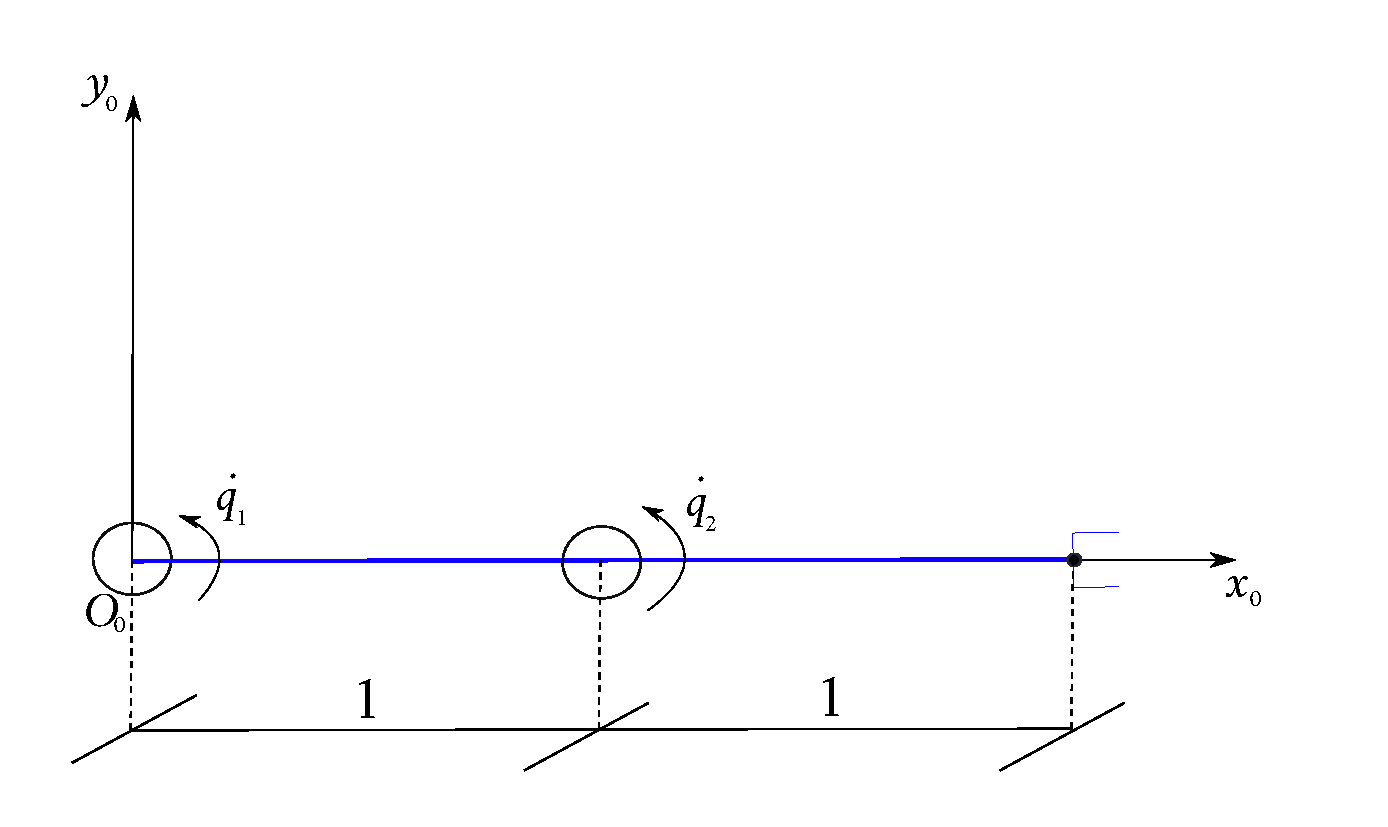
\includegraphics[scale=0.3]{manipolatoreStallo2R.pdf}
\end{center}
otteniamo
\begin{equation}
	\begin{bmatrix}
		\dot{x} \\
		\dot{y} \\
	\end{bmatrix}
	= 
	\underbrace{
	\begin{bmatrix}
		0 & 0 \\
		2 & 1 \\
	\end{bmatrix}
	}_{J_a}
	\begin{bmatrix}
		\dot{q}_1 \\
		\dot{q}_2 \\
	\end{bmatrix}
\end{equation}
calcoliamo $\mathcal{R}(J_a)$ e $\mathcal{N}(J_a^T)$,
\begin{equation}
	J_a = 
	\begin{bmatrix}
		0 & 0 \\
		2 & 1 \\
	\end{bmatrix}
	\; \Rightarrow \; \mathcal{R}(J_a) = 
	\begin{bmatrix}
		0 \\
		1 \\
	\end{bmatrix}
	\qquad 
	J_a^T = 
	\begin{bmatrix}
		0 & 2 \\
		0 & 1 \\
	\end{bmatrix}
	\; \Rightarrow \; \mathcal{N}(J_a^T) = 
	\begin{bmatrix}
		1 \\
		0 \\
	\end{bmatrix}
\end{equation}
distinguiamo due casi: il caso in cui il sistema va in stallo e quello in cui non va in stallo,
\begin{itemize}
	\item Ipotizziamo, 
	\begin{equation*}
		K =
		\begin{bmatrix}
			1 & 0 \\
			0 & 1 \\
		\end{bmatrix}
		, \qquad \underline{x}_{\,des} =  
		\begin{bmatrix}
			2 \\
			\varepsilon \\
		\end{bmatrix}
		, \qquad \underline{x} = 
		\begin{bmatrix}
			2 \\
			0 \\
		\end{bmatrix}
	\end{equation*}
	otteniamo 
	\begin{equation*}
		K \underline{e} = 
		\begin{bmatrix}
			1 & 0 \\
			0 & 1 \\
		\end{bmatrix}
		\begin{bmatrix}
			0 \\
			\varepsilon \\
		\end{bmatrix}
		=
		\begin{bmatrix}
			0 \\
			\varepsilon \\
		\end{bmatrix}
		\not\in\mathcal{N}(J_a^T)
	\end{equation*}
	in questo caso il sistema \emph{non} va in stallo.
	
	\item Cerchiamo una $\underline{x}_{\,des}$ che manda in \emph{stallo} il sistema, ovvero
	\begin{equation*}
		\underline{x}_{\,des} =
		\begin{bmatrix}
			2+\varepsilon \\
			0 \\
		\end{bmatrix},
		\qquad 
		\underline{x}_{\,des} =
		\begin{bmatrix}
			2-\varepsilon \\
			0 \\
		\end{bmatrix}
	\end{equation*}
	mandano in stallo il sistema, infatti
	\begin{equation*}
		K \underline{e} = 
		\begin{bmatrix}
			1 & 0 \\
			0 & 1 \\
		\end{bmatrix}
		\begin{bmatrix}
			\varepsilon \\
			0 \\
		\end{bmatrix}
		=
		\begin{bmatrix}
			\varepsilon \\
			0 \\
		\end{bmatrix}
		\in\mathcal{N}(J_a^T)
	\end{equation*}
\end{itemize}

\subsubsection{Interpretazione fisica}
Notiamo una interessante interpretazione fisica di questo algoritmo, tale interpretazione userà nozioni di statica spiegate in seguito. 

Supponendo che il manipolatore sia caratterizzato da una dinamica ideale $\underline{\tau} = \underline{\dot{q}}$ (masse nulle e coefficienti di attrito viscoso unitari), lo schema di inversione svolge la funzione di una \emph{molla generalizzata}, di costante $K$, che genera una forza $K \underline{e}$ che tira l'organo terminale verso la posa desiderata nello spazio operativo.

Se a tale manipolatore è concesso di muoversi, e ciò è possibile solo se $K\underline{e} \not \in \mathcal{N}(J^T)$, l'organo terminale assume la posa desiderata e possono essere individuate le variabili corrispondenti nello spazio dei giunti.

\subsection{Errore di orientamento}
Abbiamo notato che gli algoritmi per l'inversione cinematica operano su \emph{variabili di errore} che sono definite nello spazio operativo. L'errore è di tipo \emph{posizionale} o di \emph{orientamento}. Per quanto riguarda l'errore posizionale, la sua espressione è data da
\begin{equation}
	\underline{e}_{\,p} = \underline{p}_{\,d} - \underline{p}
\end{equation} 
dove $\underline{p}_{\,d}$ e $\underline{p}$ denotano rispettivamente \emph{posizione desiderata} e \emph{posizione dell'organo terminale}. La sua derivata è
\begin{equation}
	\underline{\dot{e}}_{\,p} = \underline{\dot{p}}_{\,d} - \underline{\dot{p}}
\end{equation}

\paragraph{}
Per quanto riguarda \emph{l'errore di orientamento}, la sua espressione dipende dalla rappresentazione dell'organo terminale. Scegliamo la \emph{rappresentazione Asse-Angolo}.

Indicando con  
$R_d = 
\begin{bmatrix}
	\underline{n}_d & \underline{s}_d & \underline{a}_d
\end{bmatrix}$ la matrice di rotazione della terna utensile di riferimento e con 
$R =
\begin{bmatrix}
	\underline{n} & \underline{s} & \underline{a}
\end{bmatrix}$ quella della terna utensile relativa alle variabili di giunto effettive. 

L'errore di orientamento tra le due terne può essere espresso come
\begin{equation}
	\underline{e}_{\,o} = \underline{r}\sin\vartheta
\end{equation}
dove $\underline{r}$ e $\vartheta$ caratterizzano \emph{l'asse e l'angolo} di rotazione. Sviluppando si ottiene,
\begin{equation}
	\underline{e}_{\,o} = \frac{1}{2}
	\begin{bmatrix}
		\underline{n} \times \underline{n}_{\,d} + \underline{s} \times \underline{s}_{\,d} + \underline{a} \times \underline{a}_{\,d}
	\end{bmatrix}
\end{equation}
e derivando tenendo conto di $\dot{R}(t) = S(t)R(t)$, otteniamo
\begin{equation}
	\underline{\dot{e}}_{\,o} = L^T\underline{\omega}_{\,d} - L\underline{\omega}
\end{equation}
con $L \in \mathbb{R}^{3 \times 3}$ invertibile.

\paragraph{}
Adesso studiamo la dinamica dell'errore \emph{complessiva}, 
\begin{equation*}
	\underline{\dot{e}} = 
	\begin{bmatrix}
		\underline{\dot{e}}_{\,p} \\
		\underline{\dot{e}}_{\,o} \\
	\end{bmatrix}
	=
	\begin{bmatrix}
		\underline{\dot{p}}_{\,d} - \underline{\dot{p}} \\
		L^T \underline{\omega}_{\,d} - L \underline{\omega} \\
	\end{bmatrix}
	= 
	\begin{bmatrix}
		\underline{\dot{p}}_{\,d} - J_p\underline{\dot{q}} \\
		L^T\underline{\omega}_{\,d} - LJ_o\underline{\dot{q}} \\
	\end{bmatrix}
	=
\end{equation*}
\begin{equation}
	=
	\begin{bmatrix}
		\underline{\dot{p}}_{\,d} \\
		L^T \underline{\omega}_{\,d} \\
	\end{bmatrix}
	-
	\begin{bmatrix}
		J_p\underline{\dot{q}} \\
		LJ_o\underline{\dot{q}} \\
	\end{bmatrix}
	 = 
	 \begin{bmatrix}
	 	\underline{\dot{p}}_{\,d} \\
		L^T \underline{\omega}_{\,d} \\
	 \end{bmatrix}
	 -
	 \begin{bmatrix}
	 	I & 0 \\
	 	0 & L \\
	 \end{bmatrix}
	 \underbrace{
	 \begin{bmatrix}
	 	J_p \\
	 	J_o \\
	 \end{bmatrix}
	 }_{J}
	 \underline{\dot{q}}
\end{equation}
e considerando che vogliamo un sistema asintoticamente stabile nell'origine, vogliamo che $\underline{\dot{e}}$ sia uguale ad una matrice con autovalori a parte reale negativa moltiplicata l'errore $\underline{e}$. 

Quindi, otteniamo l'espressione $\underline{\dot{e}} + K \underline{e} = \underline{0}$ seguente
\begin{equation*}
	\underline{\dot{e}} + K \underline{e} = 
	\begin{bmatrix}
		\underline{\dot{e}}_{\,p} \\
		\underline{\dot{e}}_{\,o} \\
	\end{bmatrix}
	+
	\begin{bmatrix}
		K_p & 0 \\
		0 & K_o \\
	\end{bmatrix}
	\begin{bmatrix}
		\underline{e}_{\,p} \\
		\underline{e}_{\,o} \\
	\end{bmatrix}
	=
\end{equation*}
\begin{equation}
	=
	\begin{bmatrix}
	 	\underline{\dot{p}}_{\,d} \\
		L^T \underline{\omega}_{\,d} \\
	\end{bmatrix}
	-
	\begin{bmatrix}
	 	I & 0 \\
	 	0 & L \\
	\end{bmatrix}
	J
	\underline{\dot{q}}
	+ 
	\begin{bmatrix}
		K_p \underline{e}_{\,p} \\
		K_o \underline{e}_{\,o} \\
	\end{bmatrix}
	= 
	\begin{bmatrix}
		0 \\
		0 \\
	\end{bmatrix}
\end{equation}
per analogia agli algoritmi di inversione visti fino ad ora, il legame tra $\underline{\dot{q}}$ ed $\underline{e}$ è ottenuto mediante l'inversione dello \emph{Jacobiano Geometrico} in luogo di quello \emph{Analitico}.

Calcoliamo la soluzione con inversa dello Jacobiano,
\begin{equation*}
	-
	\begin{bmatrix}
		I & 0 \\
		0 & L \\
	\end{bmatrix}
	J \underline{\dot{q}} =
	- 
	\begin{bmatrix}
		\underline{\dot{p}}_{\,d} \\
		L^T \underline{\omega}_{\,d} \\
	\end{bmatrix}	
	-
	\begin{bmatrix}
		K_p \underline{e}_{\,p} \\
		K_o \underline{e}_{\,o} \\
	\end{bmatrix}
	\quad \Rightarrow \quad
	\begin{bmatrix}
		I & 0 \\
		0 & L \\
	\end{bmatrix}
	J \underline{\dot{q}} =
	\begin{bmatrix}
		\underline{\dot{p}}_{\,d} + K_p \underline{e}_{\,p} \\
		L^T \underline{\omega}_{\,d} + K_o \underline{e}_{\,o} \\
	\end{bmatrix}
	\quad \Rightarrow
\end{equation*}
\begin{equation*}
	\Rightarrow \quad 
	J \underline{\dot{q}} = 
	\begin{bmatrix}
		I & 0 \\
		0 & L^{-1} \\
	\end{bmatrix}
	\begin{bmatrix}
		\underline{\dot{p}}_{\,d} + K_p \underline{e}_{\,p} \\
		L^T \underline{\omega}_{\,d} + K_o \underline{e}_{\,o} \\
	\end{bmatrix}
\end{equation*}
e otteniamo la soluzione per un manipolatore non ridondante e non in singolarità,
\begin{equation}
	\underline{\dot{q}} = J^{-1}
	\begin{bmatrix}
		\underline{\dot{p}}_{\,d} + K_p \underline{e}_{\,p} \\
		L^{-1}(L^T \underline{\omega}_{\,d} + K_o \underline{e}_{\,o}) \\
	\end{bmatrix}
\end{equation}
osserviamo che questa soluzione della cinematica inversa offre migliore prestazioni perchè impiegando lo Jacobiano Geometrico, si evitano l'insorgere di singolarità di rappresentazione.

Per gestire esplicitamente la \emph{singolarità} possiamo usare la \emph{pseudo-inversa smorzata} $J^*$ definita dalla ($5.15$), ottenendo la seguente soluzione,
\begin{equation}
	\underline{\dot{q}} = \underbrace{J^T(JJ^T + K^2I)^{-1}}_{J^*}  
	\begin{bmatrix}
		\underline{\dot{p}}_{\,d} + K_p \underline{e}_{\,p} \\
		L^{-1}(L^T \underline{\omega}_{\,d} + K_o \underline{e}_{\,o}) \\
	\end{bmatrix}
\end{equation}
\chapter{Statica}
L'obiettivo della statica è quello di determinare la relazione tra:
\begin{itemize}
	\item Il \emph{wrench di forza} applicato dall'organo terminale sull'ambiente esterno,
	\begin{equation}
		\underline{\gamma} = 
		\begin{bmatrix}
			\underline{f} \\
			\underline{\mu} \\
		\end{bmatrix}
	\end{equation} con $\underline{f}$ la forza risultante e $\underline{\mu}$ il momento risultante attorno all'origine della terna utensile.
	\item Le \emph{azioni generalizzate} $\underline{\tau}$ che gli attuatori devono esercitare sui giunti per equilibrare $\underline{\gamma}$. Queste azioni posso essere \emph{coppie} se si tratta di giunti rotoidali o \emph{forze} se si tratta di giunti prismatici. Notiamo che \emph{non} equilibra eventuali azioni dinamiche e nemmeno azioni gravitazionali come il peso dei link.
\end{itemize}

In pratica, vogliamo sapere quali coppie generalizzate (forze) devono essere applicate sui giunti (degli attuatori) affinché \emph{l'E-E} (End Effector) eserciti sull'ambiente un \emph{wrench} assegnato $\underline{\gamma}$.
\section{Principio dei Lavori Virtuali}
Per trovare la relazione tra $\underline{\gamma}$ e $\underline{\tau}$ utilizziamo il \emph{principio dei lavori virtuali} (PLV). Esso affermo che:

\textit{in un sistema meccanico in equilibrio, il lavoro $\delta W$ fatto da tutte le forze e coppie agenti sul sistema in conseguenza di un qualsiasi spostamento virtuale $\delta \underline{q}$ è nullo,} ovvero:
\begin{equation}
	\delta W = 0
\end{equation}
uno spostamento virtuale è un piccolo cambiamento di configurazione $\delta \underline{q}$ compatibile con i vincoli esistenti. 

In generale, $\delta \underline{q} \neq d\underline{q}$, perchè non sempre uno spostamento elementare $d\underline{q}$ del sistema è compatibile con i vincoli esistenti. Ma nel caso di un robot a base fissa, tutte le componenti di uno spostamento virtuale sono indipendenti e pertanto un qualsiasi spostamento elementare arbitrario $d\underline{q}$ è anche uno spostamento virtuale $\delta \underline{q}$.

\paragraph{}
Le \textbf{azioni} (forze o coppie) che compiono lavoro in conseguenza di uno spostamento virtuale del robot $\delta \underline{q} = d\underline{q}$ sono:
\begin{itemize}
	\item Le azioni $\underline{\tau}$ degli attuatori sui giunti, i quali subiscono uno spostamento $d \underline{q}$.
	\item Il \emph{wrench} di forza pari a $-\gamma$ applicato sull'organo terminale, perchè se $\gamma$ è l'azione del manipolatore sull'ambiente, allora per il principio di azione e reazione, $-\gamma$ è l'azione dell'ambiente sul manipolatore.
\end{itemize}

\paragraph{}
Il \emph{lavoro virtuale} delle azioni $\underline{\tau}$ vale:
\begin{equation}
	\delta W_{\underline{\tau}} = \sum_{i = 1}^n \tau_i \delta q_i = \underline{\tau}^T \delta \underline{q}
\end{equation}

\paragraph{}
Il \emph{lavoro virtuale} delle azioni $-\underline{\gamma}$ vale:
\begin{equation*}
	\delta W_{- \underline{\gamma}} = \delta W_{- \underline{f}} + \delta W_{- \underline{\mu}} = - \underline{f}^T \delta \underline{p} - \underline{\mu}^T \underline{\omega} \delta t =
\end{equation*}
\begin{equation}
	= - \underline{f}^T J_p \delta \underline{q} - \underline{\mu}^T J_o \underbrace{\underline{\dot{q}} \delta t}_{\delta \underline{q}}  
\end{equation}

\paragraph{}
Il \emph{lavoro virtuale complessivo} risulta essere:
\begin{equation}
	\delta W = \delta W_{\underline{\tau}} + \delta W_{- \underline{\gamma}} = \delta W_{\underline{\tau}} + \delta W_{- \underline{f}} + \delta W_{- \underline{\mu}} = 0
\end{equation}
pertanto, 
\begin{equation}
	\underline{\tau}^T \delta \underline{q} - \underline{f}^T J_p \delta \underline{q} - \mu^T J_o \delta \underline{q} = \delta \underline{q} ( \underline{\tau}^T - \underline{f}^T J_p - \underline{\mu}^T J_o) = 0
\end{equation}
e otteniamo
\begin{equation}
	\delta \underline{q} \Biggl( \underline{\tau}^T - 
	\begin{bmatrix}
		\underline{f}^T & \underline{\mu}^T
	\end{bmatrix}
	\begin{bmatrix}
		J_p \\
		J_o \\
	\end{bmatrix}
    \Biggr) = \delta \underline{q} \Bigl( \underline{\tau}^T - \underline{\gamma}^TJ \Bigr) = 0 \; \Rightarrow \; \underline{\tau}^T - \underline{\gamma}^T J = 0
\end{equation}
quindi,
\begin{equation}
	\underline{\tau} = J^T \underline{\gamma} \quad \forall \delta \underline{q}
\end{equation}

\section{Dualità Cinetostatica}
La relazione statica ($6.8$), combinata con la relazione cinematica differenziale ($4.12$), mette in luce una proprietà di \emph{dualità cineto-statica}. Infatti, considerando la seguente rappresentazione 

\begin{center}
	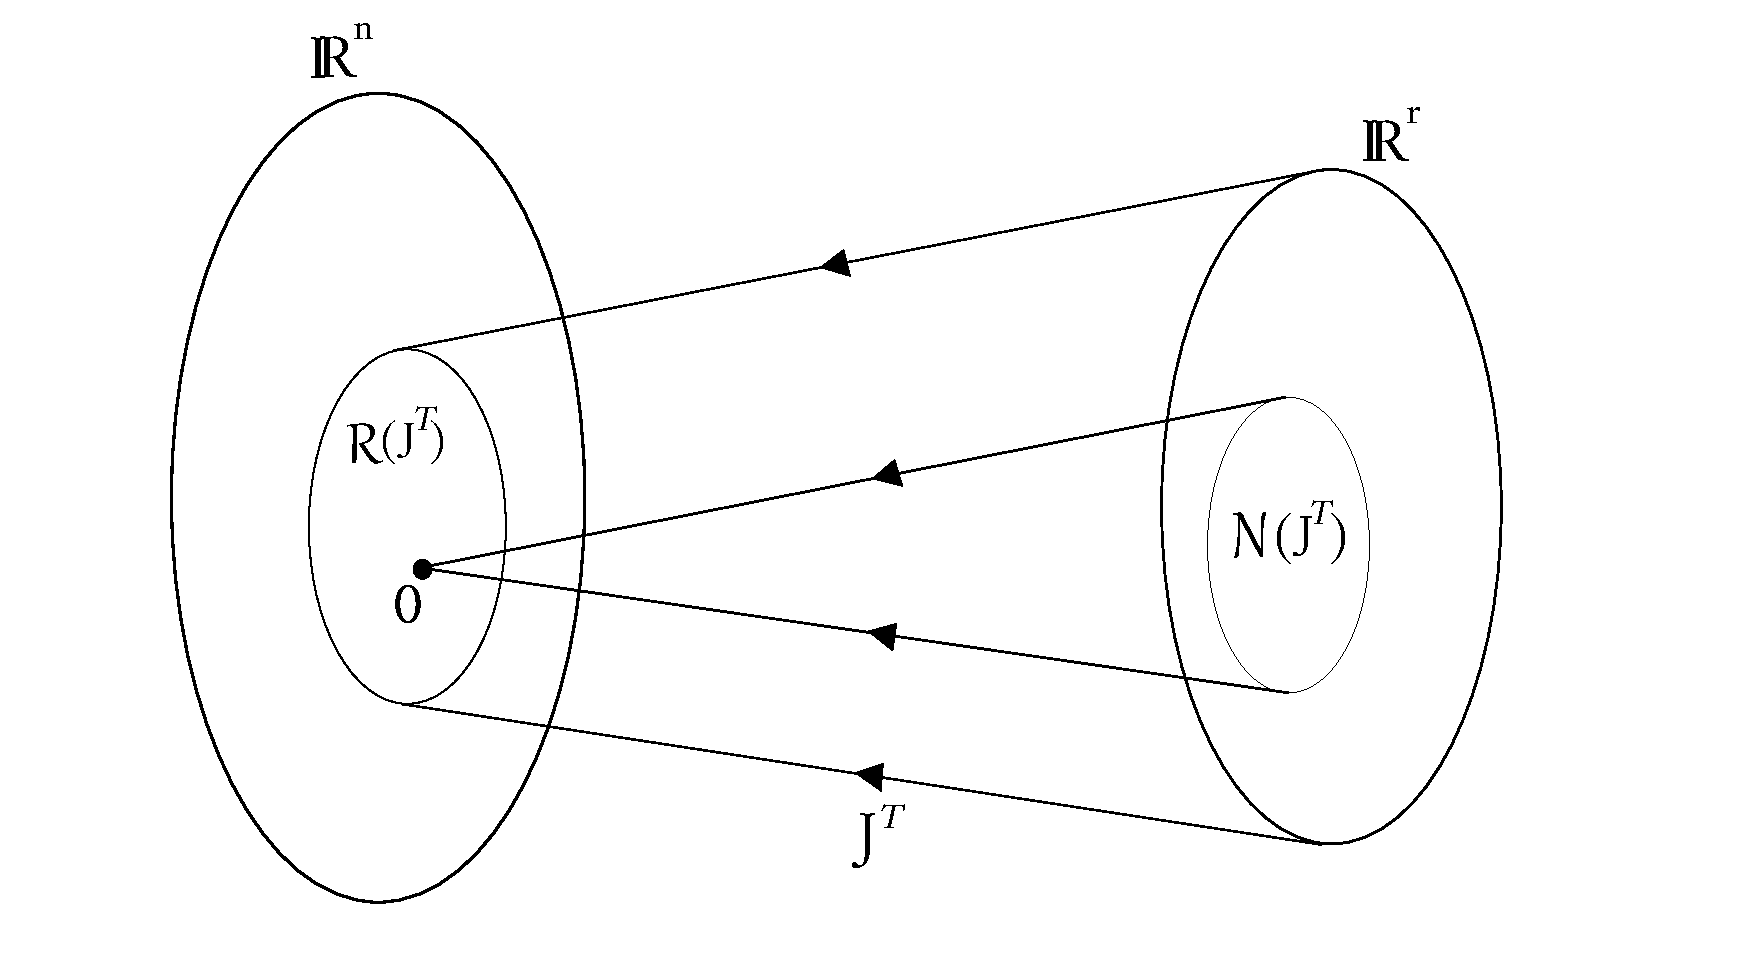
\includegraphics[scale=0.35]{dualitaCinetostatica.pdf}
	\caption{Relazione tra spazio delle forze all'organo terminale e spazio delle coppie ai giunti.}
\end{center}

si ottiene che:
\begin{itemize}
	\item L'immagine di $J^T$ è il sottospazio $\mathcal{R}(J^T)$ in $\mathbb{R}^n$ che individua le coppie ai giunti che possono bilanciare le forze all'organo terminale, nella configurazione assegnata al manipolatore.
	\item Il nullo di $J^T$ è il sottospazio $\mathcal{N}(J^T)$ in $\mathbb{R}^r$ a cui appartengono le forze all'organo terminale che non richiedono alcuna coppia di bilanciamento ai giunti, nella configurazione assegnata al manipolatore.
\end{itemize}
Notiamo che le forze all'organo terminale $\underline{\gamma} \in \mathcal{N}(J^T)$ sono interamente assorbite dalla struttura, nel senso che le reazioni vincolari sono in grado di bilanciarle esattamente.

\subsubsection{Relazione $\mathcal{N}(J^T) \perp \mathcal{R}(J)$}
La relazione tra i diversi sottospazi sono regolate da:
\begin{equation}
	\mathcal{N}(J) = \mathcal{R}^{\perp}(J^T) \qquad \mathcal{R}(J) = \mathcal{N}^{\perp}(J^T)
\end{equation}
ovvero, i due sottospazi sono legati dall'operazione di \emph{complemento ortogonale}. Dimostriamo questo legame procedendo per \emph{assurdo}:
\paragraph{}
\textit{
Sia $\underline{y}_{\,1} \in \mathcal{R}(J)$, $\underline{y}_{\,2} \in \mathcal{N}(J^T)$, con $\underline{y}_{\,1} = J \underline{\dot{q}}_{\,1}$. Supponiamo che $\underline{y}_{\,1}$ e $\underline{y}_{\,2}$ non siano ortogonali, ovvero che
\begin{equation}
	\underline{y}_{\,1}^T \underline{y}_{\,2} \neq 0
\end{equation} 
ma sappiamo che 
\begin{equation}
	\underline{y}_{\,1}^T \underline{y}_{\,2} = \underline{\dot{q}}_{\,1}^T J^T \underline{y}_{\,2}
\end{equation}
pertanto, dovrebbe valere $\underline{\dot{q}}_{\,1}^T J^T \underline{y}_{\,2} \neq 0$, e ciò significa che 
\begin{equation}
	J^T \underline{y}_{\,2} \neq 0
\end{equation}
e sapendo che $\underline{y}_{\,2} \in \mathcal{N}(J^T)$ la relazione ($6.12$) risulta impossibile, ed ecco l'assurdo.}
\chapter{Azionamenti}
\paragraph{}
Il moto imposto al generico giunto del manipolatore è realizzato mediante un \emph{sistema di attuazione} che, in linea di principio, è costituito da:
\begin{itemize}
	\item una \emph{sorgente di alimentazione},
	\item un \emph{amplificatore di potenza},
	\item un \emph{servomotore},
	\item un \emph{organo di trasmissione}. 
\end{itemize}

Spieghiamo il funzionamento degli \emph{azionamenti elettrici} per l'attuazione dei giunti di un manipolatore. Partiamo dai \emph{modelli matematici} che descrivono il comportamento dinamico e successivamente ricaviamo gli \emph{schemi a blocchi} che consentono di evidenziare le caratteristiche di controllo.

Iniziamo col modello elettrico modellando il motore a corrente continua attraverso lo schema seguente,
\begin{center}
	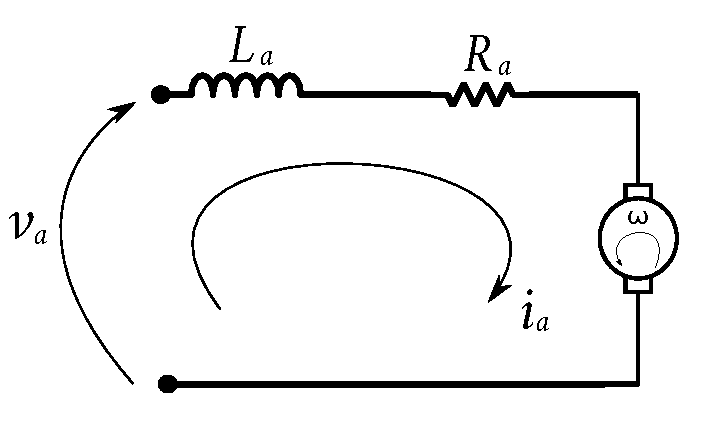
\includegraphics[scale=0.35]{circuitoMotore.pdf}
	\caption{Modello elettrico.}
\end{center}

scriviamo le equazioni che descrivono l'equilibrio elettrico del circuito nel dominio della variabile $s$,
\begin{equation}
	V_a = s L_a I_a + R_a I_a + k_v \Omega
\end{equation}
dove $V_a$ e $I_a$ rappresentano tensione e corrente applicate al circuito di armatura di resistenza $R_a$ e induttanza $L_a$, e $k_t \Omega$ rappresenta la forza controelettromotrice (FCEM) proporzionale alla velocità di rotazione $\Omega$ attraverso la costante di tensione $k_v$.

Proseguiamo col modello meccanico scrivendo le equazioni dell'equilibrio meccanico,
\begin{equation}
	\begin{cases}
		C_m = sI_m \Omega + F_m \Omega + D_l \\
		C_m = k_t I_a \\
	\end{cases}	
\end{equation}
dove $C_m$ rappresenta la coppia motrice elettromeccanica, $D_l$ il disturbo di coppia di carico, $I_m$ e $F_m$ sono il momento di inerzia e il coefficiente di attrito viscoso del motore e $k_t$ la costante di coppia, che in genere vale $k_t = k_v$.
\paragraph{}
Per quanto riguarda \emph{l'amplificatore di potenza}, ad esso viene associata la seguente relazione \emph{I/U}:
\begin{equation}
	\frac{V_a}{V_c} = \frac{G_v}{1 + sT_v}
\end{equation}
dove $G_v$ rappresenta il guadagno in tensione e $T_v$ una costante di tempo.
\paragraph{}
Lo schema a blocchi \emph{dell'amplificatore di potenza} e \emph{servomotore} è il seguente,
\begin{center}
	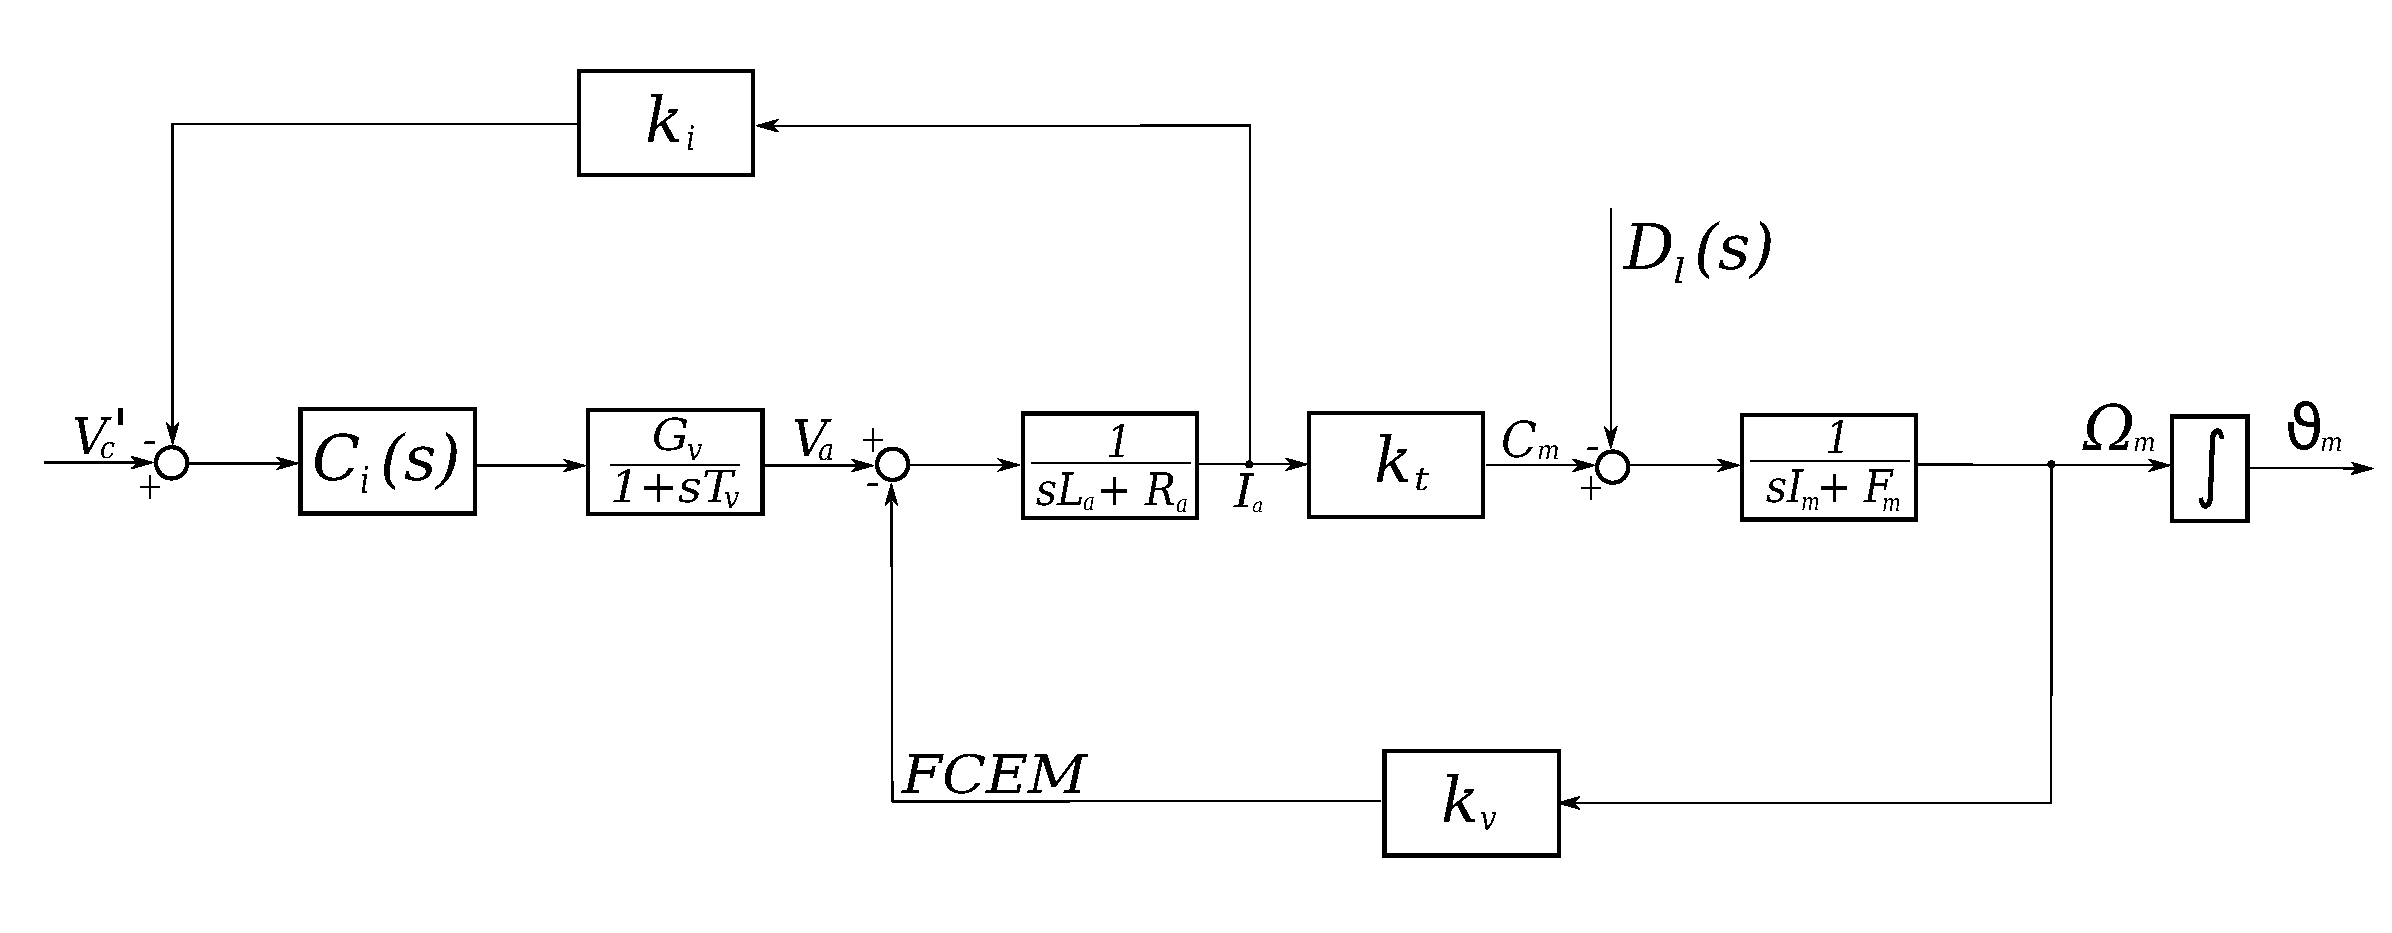
\includegraphics[scale=0.3]{schemaAzionamentoElettrico.pdf}
	\caption{Schema a blocchi di un azionamento elettrico.}
\end{center}
notiamo:
\begin{itemize}
	\item Vi è una \textbf{\emph{retroazione di corrente}} di armatura misurata tramite un trasduttore di costante $k_i$ inserito tra l'amplificatore di potenza e il circuito di armatura della macchina.
	\item Vi è un \textbf{\emph{regolatore di corrente}} $C_i(s)$ che consente di ottenere caratteristiche dell'azionamento particolari in base ai guadagni d'anello.
	\item $V'_c$ è un \textbf{\emph{riferimento di corrente}} e mediante un'opportuna scelta di $C_i(s)$ il ritardo tra corrente $I_a$ e tensione $V'_c$ risulta minore rispetto a quello tra $I_a$ e $V_c$.
\end{itemize}

\section{Pilotaggio}
Il pilotaggio di questo sistema può avvenire in due modi: \emph{pilotaggio in tensione} e \emph{pilotaggio in corrente}. 

\subsubsection{Pilotaggio in tensione}
Ricaviamo la \emph{funzione di trasferimento} considerando le seguenti equazioni e tralasciando il disturbo $D_l(s)$,
\begin{equation}
	\begin{cases}
		v_a(t) = L_a \frac{d i_a}{dt} + R_a i_a + k_v \omega \\
		c_m(t) = I_m \dot{\omega} + F_m \omega \\
		c_m(t) = k_t i_a \\
	\end{cases}
	\quad\longleftrightarrow\quad 
	\begin{cases}
		V_a(s) = (sL_a + R_a)I_a(s) + k_v \Omega(s) \\
		k_t I_a(s) = (sI_m + F_m) \Omega(s) \\
	\end{cases}
\end{equation}
ottenendo,
\begin{equation}
	\frac{\Omega(s)}{V_a(s)} = \frac{k_t}{(sL_a + R_a)(sI_m + F_m) + k_v k_t}
\end{equation}

Elaborando l'espressione della \emph{f.d.t} ottenuta eseguendo i prodotti e dividendo per $k_vk_t$ risulta
\begin{equation}
	\frac{\Omega(s)}{V_a(s)} = \frac{\frac{1}{k_v}}{\frac{L_a I_m s^2}{k_v k_t} + (\frac{R_a I_m}{k_v k_t} + \frac{L_a F_m}{k_v k_t})s + \frac{R_aF_m}{k_v k_t} + 1}
\end{equation}
e definiamo le seguenti costanti:
\begin{itemize}
	\item $\tau_m = \frac{R_a I_m}{k_v k_t}$ la \emph{costante di tempo meccanica}.
	\item $\tau_v = \frac{L_a}{R_a}$ la \emph{costante di tempo elettrica}.
	\item $\gamma = \frac{R_a F_m}{k_v k_t}$ parametro adimensionale con $\frac{k_vk_t}{R_a}$ \emph{attrito elettrico}.
\end{itemize}
ottenendo la riscrittura di ($7.6$)
\begin{equation}
	\frac{\Omega(s)}{V_a(s)} = \frac{\frac{1}{k_v}}{\tau_v \tau_m s^2 +  (\gamma \tau_v + \tau_m)s + \gamma +1}
\end{equation}
considerando $\gamma$ trascurabile (ad esempio nei motori commerciali $\gamma \ll 1$) otteniamo
\begin{equation}
	\frac{\Omega(s)}{V_a(s)} = \frac{\frac{1}{k_v}}{\tau_v \tau_m s^2 + \tau_m s + 1} = \frac{\frac{1}{k_v}}{(\tau_v s + 1)(\tau_m s + 1)}
\end{equation}
ottenendo due sistemi del primo ordine in serie.

Infine, quando la dinamica è molto veloce possiamo ottenere un'ulteriore approssimazione
\begin{equation}
	\frac{\Omega(s)}{V_a(s)} \approx \frac{\frac{1}{k_v}}{(\tau_m s + 1)}
\end{equation}

\subsubsection{Pilotaggio in corrente}
Ricaviamo la \emph{funzione di trasferimento} considerando le seguenti equazioni e tralasciando il disturbo $D_l(s)$,
\begin{equation}
	\begin{cases}
		c_m(t) = k_t i_a \\
		c_m(t) = I_m \dot{\omega} + F_m \omega \\
	\end{cases}
	\quad \longleftrightarrow \quad 
	\begin{cases}
		C_m(s) = k_t I_a(s) \\
		C_m(s) = (sI_m + F_m) \Omega(s) \\ 
	\end{cases}
\end{equation}
ottenendo
\begin{equation}
	\frac{\Omega(s)}{I_a(s)} = \frac{k_t}{sI_m + F_m}
\end{equation}

Elaborando l'espressione della \emph{f.d.t} ottenuta eseguendo la divisione dell'attrito $F_m$ risulta
\begin{equation}
	\frac{\Omega(s)}{I_a(s)} = \frac{\frac{k_t}{F_m}}{\frac{I_m}{F_m}s + 1}
\end{equation}
con $\frac{I_m}{F_m}$ costante di tempo meccanica.

\section{Azionamenti del sistema}
Esaminando lo schema in Figura $7.2$ notiamo che come già detto, la scelta del regolatore $C_i(s)$ dell'anello di corrente consente di ottenere, in base ai valori assunti dai guadagni d'anello, due tipi di azionamenti. 
\begin{itemize}
	\item \textbf{Azionamento in tensione} se $k_i = 0$.
	\item \textbf{Azionamento in corrente} se $k_i \neq 0$.
\end{itemize}

\subsubsection{\underline{Azionamento in tensione}}
In questo caso poniamo $k_i = 0$, supponiamo unitaria la costante di guadagno $C_i(s)$ e trascuriamo $D_l(s)$. 

Considerando che la frequenza di interesse è la \emph{bassa frequenza}, ciò implica le seguenti semplificazioni:
\begin{equation}
	\frac{1}{sL_a + R_a} \simeq \frac{1}{R_a}, \quad \frac{G_v}{sT_v + 1} \simeq G_v, \quad \frac{\frac{1}{k_v}}{s \tau_m + 1} \simeq \frac{1}{k_v}
\end{equation}

inoltre considerando che l'attrito meccanico viene trascurato rispetto l'attrito elettrico ($F_m \ll \frac{k_v k_t}{R_a}$)otteniamo,
\begin{equation}
	\begin{cases}
		V_a(s) = C_i(s) \frac{G_v}{sT_v + 1} V'_c \simeq G_v V'_c(s)\\
		C_m(s) = \frac{k_t}{R_a}\Bigl( G_v V'_c(s) - k_v \Omega(s) \Bigr) \\
		\Omega(s) = \frac{k_t}{R_a} \frac{1}{sI_m + F_m} \Bigl( G_v V'_c(s) - k_v \Omega(s) \\
	\end{cases}
\end{equation}
e scriviamo
\begin{equation}
	 \Omega(s) \Bigl( 1 + \frac{k_v k_t}{R_a} \frac{1}{sI_m + F_m} \Bigr) = \frac{k_t}{R_a} \frac{1}{sI_m + F_m} G_v V'_c(s)
\end{equation}
sviluppando il termine in parentesi ed eliminando i termini trascurabili (come $R_aF_m$), otteniamo la seguente espressione
\begin{equation}
	\Omega(s) \Bigl( R_a I_ms + k_v k_t \Bigr) = k_t G_v V'_c(s) \quad \Rightarrow \quad \Omega(s) = \frac{k_t}{R_a I_ms + k_v k_t} G_v V'_c(s)
\end{equation}
dividendo per $k_v k_t$ e considerando la \emph{bassa frequenza} otteniamo la seguente \emph{f.d.t.}
\begin{equation}
	\Omega(s) = \frac{\frac{1}{k_v}}{\frac{R_a I_m s}{k_v k_t} + 1} G_v V'_c(s) = \frac{\frac{1}{k_v}}{s\tau_m + 1} G_v V'_c(s) \simeq \frac{1}{k_v} G_v V'_c(s)
\end{equation}
e quindi l'azionamento assume caratteristiche di \emph{generatore controllato di velocità} espresso in figura,
\begin{center}
	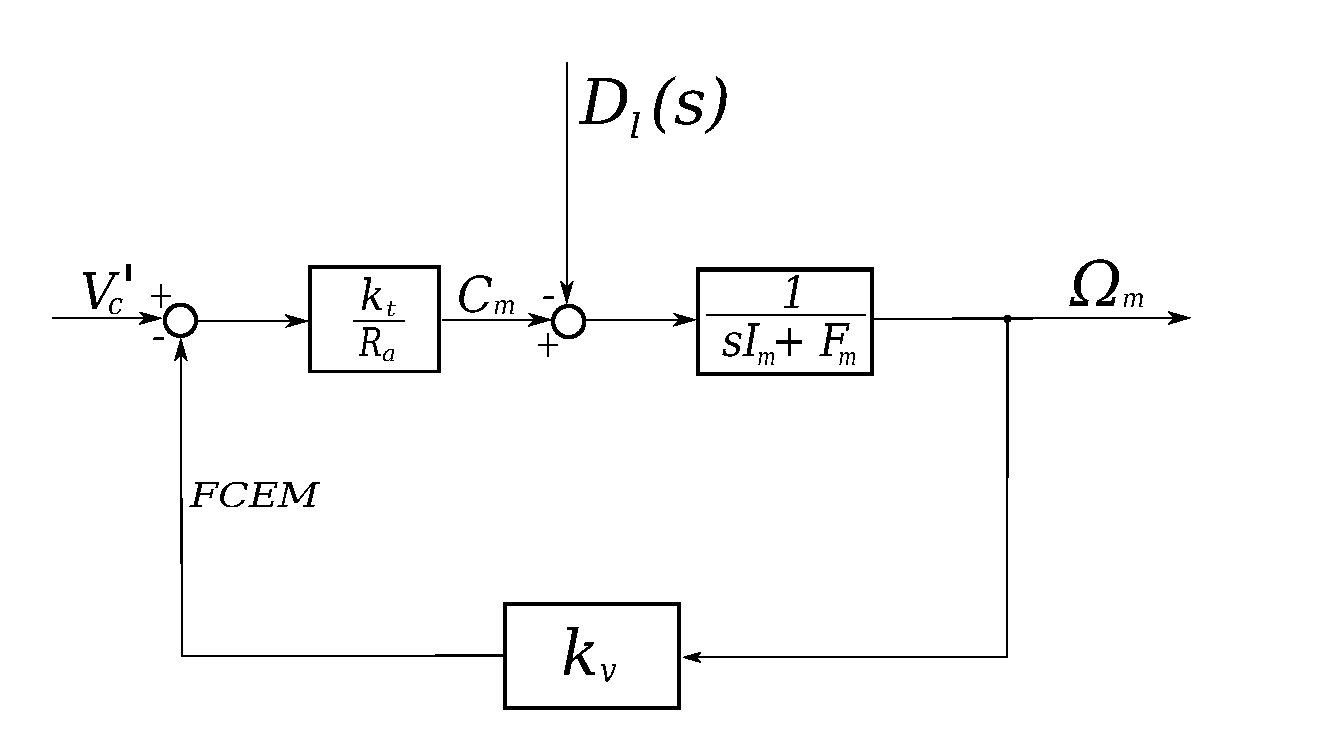
\includegraphics[scale=0.3]{schemaAzionamentoInTensione.pdf}
	\caption{Schema a blocchi dell'azionamento controllato in tensione.}
\end{center}

\subsubsection{\underline{Azionamento in corrente}}
In questo caso poniamo $k_i \neq 0$, supponiamo unitaria la costante di guadagno $C_i(s)$ così da avere \emph{un'azione integrale} e trascuriamo $D_l(s)$. La presenza di tale azione integrale ci da la possibilità di reiettare completamente a regime un disturbo di velocità costante. Infatti la FCEM $k_v \Omega(s)$ entra come un disturbo nell'anello di corrente.

Scriviamo la \emph{f.d.t.} di questo disturbo di velocità su $I_a(s)$
\begin{equation}
	\frac{I_a(s)}{k_v \Omega(s)} = \frac{-\frac{1}{R_a}}{1 + L(s)} = \frac{-\frac{1}{R_a}}{k_i C_i(s) \frac{G_v}{sT_v + 1} \frac{1}{R_a}}
\end{equation}
considerando le seguenti semplificazioni
\begin{itemize}
	\item $L(s)\vert_{s = 0} = \frac{G_v k_i}{R_a}$ dovuta alla \emph{bassa frequenza}.
	\item $G_v k_i \gg R_a$ a causa dell'elevato valore di $G_v$.
\end{itemize}
e otteniamo
\begin{equation}
	\frac{I_a(s)}{k_v \Omega(s)} \simeq \frac{\frac{1}{R_a}}{1 + G_v \frac{k_i}{R_a}} \simeq \frac{\frac{1}{R_a}}{G_v \frac{k_i}{R_a}} = \frac{1}{G_v k_i}
\end{equation}

Calcolando la \emph{f.d.t.} dell'anello di corrente con tutte le semplificazioni fatte sopra otteniamo
\begin{equation}
	\frac{I_a(s)}{V'_c(s)} = \frac{C_i(s) \frac{G_v}{sT_v + 1} \frac{1}{R_a}}{1 + k_i C_i(s) \frac{G_v}{s T_v + 1} \frac{1}{R_a}} \simeq \frac{1}{k_i}
\end{equation}
si ottiene un \emph{generatore controllato di coppia} espresso in figura,
\begin{center}
	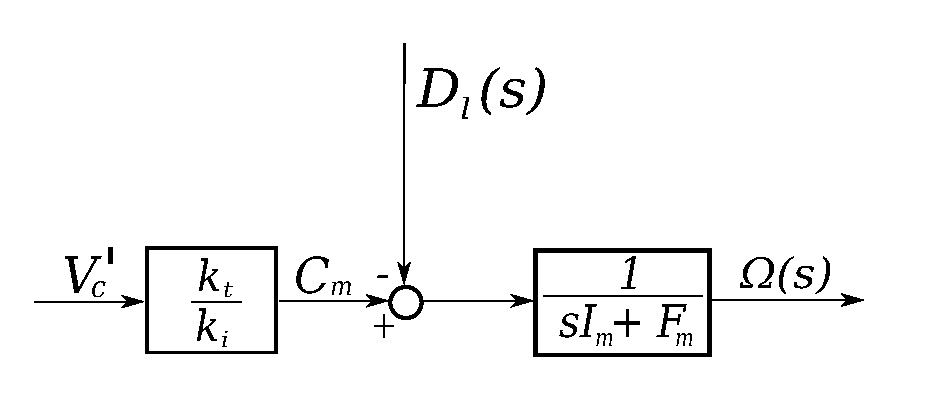
\includegraphics[scale=0.35]{schemaAzionamentoInCorrente.pdf}
	\caption{Schema a blocchi dell'azionamento controllato in corrente}
\end{center}

\section{Effetti del disturbo $D_l(s)$}
Fino adesso abbiamo trascurato il disturbo $D_l(s)$, andiamo a calcolarci l'effetto del disturbo di coppia $D_l(s)$ su $\Omega(s)$ distinguendo opportunamente i due casi.

\subsubsection{Azionamento con $k_i = 0$:}
Calcoliamo l'effettiva $\Omega(s)$ così da vedere l'effetto di $D_l(s)$,
\begin{equation}
	\Omega(s) = G_v V'_c \frac{\frac{1}{k_v}}{s \tau_m + 1} - D_l(s) \frac{\frac{1}{sI_m + F_m}}{1 + \frac{k_v k_t}{R_a (s I_m) + F_m}} = G_v V'_c \frac{\frac{1}{k_v}}{s \tau_m + 1} - D_l(s) \frac{R_a}{s R_a I_m + R_a F_m + k_v k_t}
\end{equation}
considerando che $R_aF_m$ è trascurabile, otteniamo
\begin{equation}
	\Omega(s) = G_v V'_c \frac{\frac{1}{k_v}}{s \tau_m + 1} - D_l(s) \frac{\frac{R_a}{k_vk_t}}{\frac{R_aI_m}{k_vk_t}s + 1}
\end{equation}
con $\frac{R_a}{k_vk_t}$ una quantità piccola e $\frac{R_aI_m}{k_vk_t} = \tau_m$.

Otteniamo così la \emph{f.d.t.} tra il disturbo e l'uscita
\begin{equation}
	\frac{\Omega(s)}{D_l(s)} = - \frac{\frac{R_a}{k_v k_t}}{s\tau_m + 1}
\end{equation}

\subsubsection{Azionamento con $k_i \neq 0$:}
Calcoliamo l'effettiva $\Omega(s)$ così da vedere l'effetto di $D_l(s)$,
\begin{equation}
	\Omega(s) = \frac{\frac{k_v}{k_i}}{sI_m + F_m} V'_c(s) - \frac{1}{sI_m + F_m} D(s) = \frac{\frac{k_t}{k_v} \frac{1}{F_m}}{s \frac{I_m}{F_m}+1} V'_c(s) - \frac{\frac{1}{F_m}}{s\frac{I_m}{F_m} + 1}D_l(s)
\end{equation}
con $\frac{1}{F_m} \gg \frac{R_a}{k_v k_t}$ e $\frac{I_m}{F_m} \gg \frac{R_a I_m}{F_m}$.

Otteniamo così la \emph{f.d.t.} tra il disturbo e l'uscita
\begin{equation}
	\frac{\Omega(s)}{D_l(s)} = - \frac{\frac{1}{F_m}}{s\frac{I_m}{F_m} + 1}
\end{equation}
\chapter{Dinamica dei Robot}
Questo capitolo si occupa di scrivere le equazioni del moto di un robot manipolatore a catena aperta semplice facendo uso delle equazioni di Lagrange. Scrivere le equazioni del moto vuol dire esprimere le azioni degli attuatori che fanno muovere il meccanismo in funzione di
\begin{equation}
	\underline{q}, \; \dot{\underline{q}}, \; \ddot{\underline{q}}, \; \underline{\gamma}
\end{equation}
con $\underline{q}$ coordinate lagrangiane e $\underline{\gamma}$ eventuali azioni che il meccanismo esercita sull'ambiente esterno, come spostare un peso con l'organo terminale.

Un obiettivo rilevante dello studio della dinamica dei robot è quello della progettazione degli algoritmi di controllo che si basano sulla conoscenza delle forze agli attuatori ricavati dal modello dinamico.
\paragraph{}
Scrivere le equazioni del moto di un meccanismo vuol dire esplicitare la \emph{funzione di dinamica inversa},
\begin{equation}
	\underline{\tau} = \underline{\tau}(\underline{q}, \underline{\dot{q}}, \underline{\ddot{q}}, \underline{\gamma})
\end{equation}
dove $\underline{\tau}$ è il vettore delle azioni che gli attuatori esercitano sui giunti (forze o coppie).


Il modello dinamico può essere facilmente invertito ricavando la \emph{funzione di dinamica diretta},
\begin{equation}
	\underline{\ddot{q}} = \underline{\ddot{q}}(\underline{q}, \underline{\dot{q}}, \underline{\tau}, \underline{\gamma}).
\end{equation} 

\subsubsection{Tecniche:}
Esistono due metodi per ricavare le equazioni del moto,
\begin{enumerate}
	\item La \textbf{formulazione di Lagrange}: si basa sulle equazioni di Lagrange ricavate nelle \emph{Appendici}, ha l'enorme vantaggio di essere \emph{sistematica}, fornisce le equazioni del moto in forma analitica e compatta che evidenzia la matrice di inerzia, matrice delle forze centrifughe e di Coriolis e il vettore delle forze gravitazionale. Utile per progettare un sistema di controllo.
	\item La \textbf{formulazione di Newton-Eulero}: è intrinsecamente un metodo ricorsivo che risulta efficace da un punto di vista computazionale, infatti sfrutta la natura seriale a catena aperta tipica del manipolatore. Questo metodo non viene trattato in queste dispense.
\end{enumerate}

\subsubsection{Dinamica diretta e inversa:}
Vediamo le sostanziali differenze tra le due,
\begin{itemize}
	\item La \textbf{Dinamica diretta} consiste nel determinare, le accelerazioni risultanti ai giunti $\ddot{\underline{q}}$, assegnate $\underline{\tau}$ ed eventualmente $\underline{\gamma}$ e note le posizioni $\underline{q}$ e le velocità $\dot{\underline{q}}$ dei giunti.
	\item La \textbf{Dinamica inversa} consiste nel determinare le azioni degli attuatori $\underline{\tau}$ necessarie alla generazione del movimento specificato assegnando le accelerazioni, velocità e posizioni dei giunti e note le eventuali forze all'organo terminale $\underline{\gamma}$.
\end{itemize}

Al livello computazionale, per un manipolatore a $n$ giunti, il numero di operazioni richieste dal calcolo della dinamica risulta pari a $O(n^2)$ per la dinamica diretta e $O(n)$ per la dinamica inversa. 

\section{Formulazione di Lagrange}
Con la \emph{formulazione di Lagrange}, le equazioni del moto possono essere ricavate con un approccio indipendente dal sistema di coordinate di riferimento. Scelto un insieme di variabili $q_i$ per $i = 1, \cdots, n$, denominate \emph{coordinate lagrangiane o generalizzate} che descrivono le posizioni degli elementi meccanici costituenti il manipolatore a $n$ gradi di libertà, si definisce \emph{lagrangiana} del sistema meccanico la funzione
\begin{equation}
	\mathcal{L}(\underline{\dot{q}}, \underline{q}, t) = T(\underline{\dot{q}}, \underline{q}, t) - U(\underline{q}, t)
\end{equation} 
in cui $T$ ed $U$ sono le rispettivamente l'energia cinetica e l'energia potenziale totali del sistema.

La scelta delle coordinate lagrangiane non è unica ma, per i robot a catena aperta che trattiamo, è ovvio scegliere come coordinate lagrangiane gli elementi del vettore $\underline{q}$ delle coordinate dei giunti, si tratta quindi di rotazioni $\theta_i$ o traslazioni $d_i$.

\paragraph{}
Notiamo che tra le coordinate lagrangiane di un robot con base fissa che si muove liberamente nello spazio non esistono vincoli al livello differenziale, ovvero tra le derivate temporali di $\underline{q}$, pertanto sono sistemi meccanici con vincoli \emph{olonomi}, o in breve, \emph{sistemi olonomi}. Pertanto possiamo scrivere le $n$ equazioni di Lagrange,
\begin{equation}
	\frac{d}{dt} \Biggl( \frac{\partial \mathcal{L}}{\partial \dot{q}_i} \Biggr) - \frac{\partial \mathcal{L}}{\partial q_i} = Q_i \qquad \forall i = 1, \cdots, n
\end{equation}
dove $Q_i$ indica la componente lagrangiana delle forze attive \emph{non conservative} lungo la direzione della coordinata lagrangiana $q_i$. Bisogna puntualizzare però, che riferendoci ad un robot, le forze non conservative $Q_i$ sono composto in linea del tutto generale da:
\begin{itemize}
	\item \emph{Forza che gli attuatori esercitano sul giunto} $i$: Ovvero, $\underline{\tau}_{\,i}$
	\item \emph{Forza di attrito agente sul giunto} $i$: ovvero, $\underline{\tau}_{\,i,f}$
	\item \emph{Effetti delle forze esterne sul giunto} $i$: ovvero, $-J_i^T \underline{\gamma}$
\end{itemize}
pertanto, il secondo membro della $8.5$, in del tutto generale assume la forma 
\begin{equation*}
	Q_i = \underline{\tau}_{\,i}-\underline{\tau}_{\,i,f} - J_i^T \underline{\gamma}
\end{equation*}

Le $n$ equazioni in $(8.5)$ rappresentano le \emph{equazioni del moto} del manipolatore.

\subsection{Motoriduttore con pendolo in gravità}
Per capire meglio questo metodo, facciamo un esempio e applichiamo il metodo delle equazioni di Lagrange ad un pendolo, mobile nel piano verticale, azionato da un motoriduttore. La procedura è semplice,
\begin{enumerate}
	\item Calcoliamo l'energia cinetica del sistema $T$.
	\item Calcoliamo l'energia potenziale del sistema $U$.
	\item Calcoliamo la Lagrangiana $\mathcal{L} = T-U$.
	\item Infine, deriviamo la Lagrangiana secondo la $(8.5)$ e otteniamo le equazioni del moto.
\end{enumerate} 
il pendolo di massa $m$ giace sul piano $xy$ e possiede tensore di inerzia baricentrico $I_l$ e un tensore di inerzia del motoriduttore pari a $I_m$. 
\begin{center}
	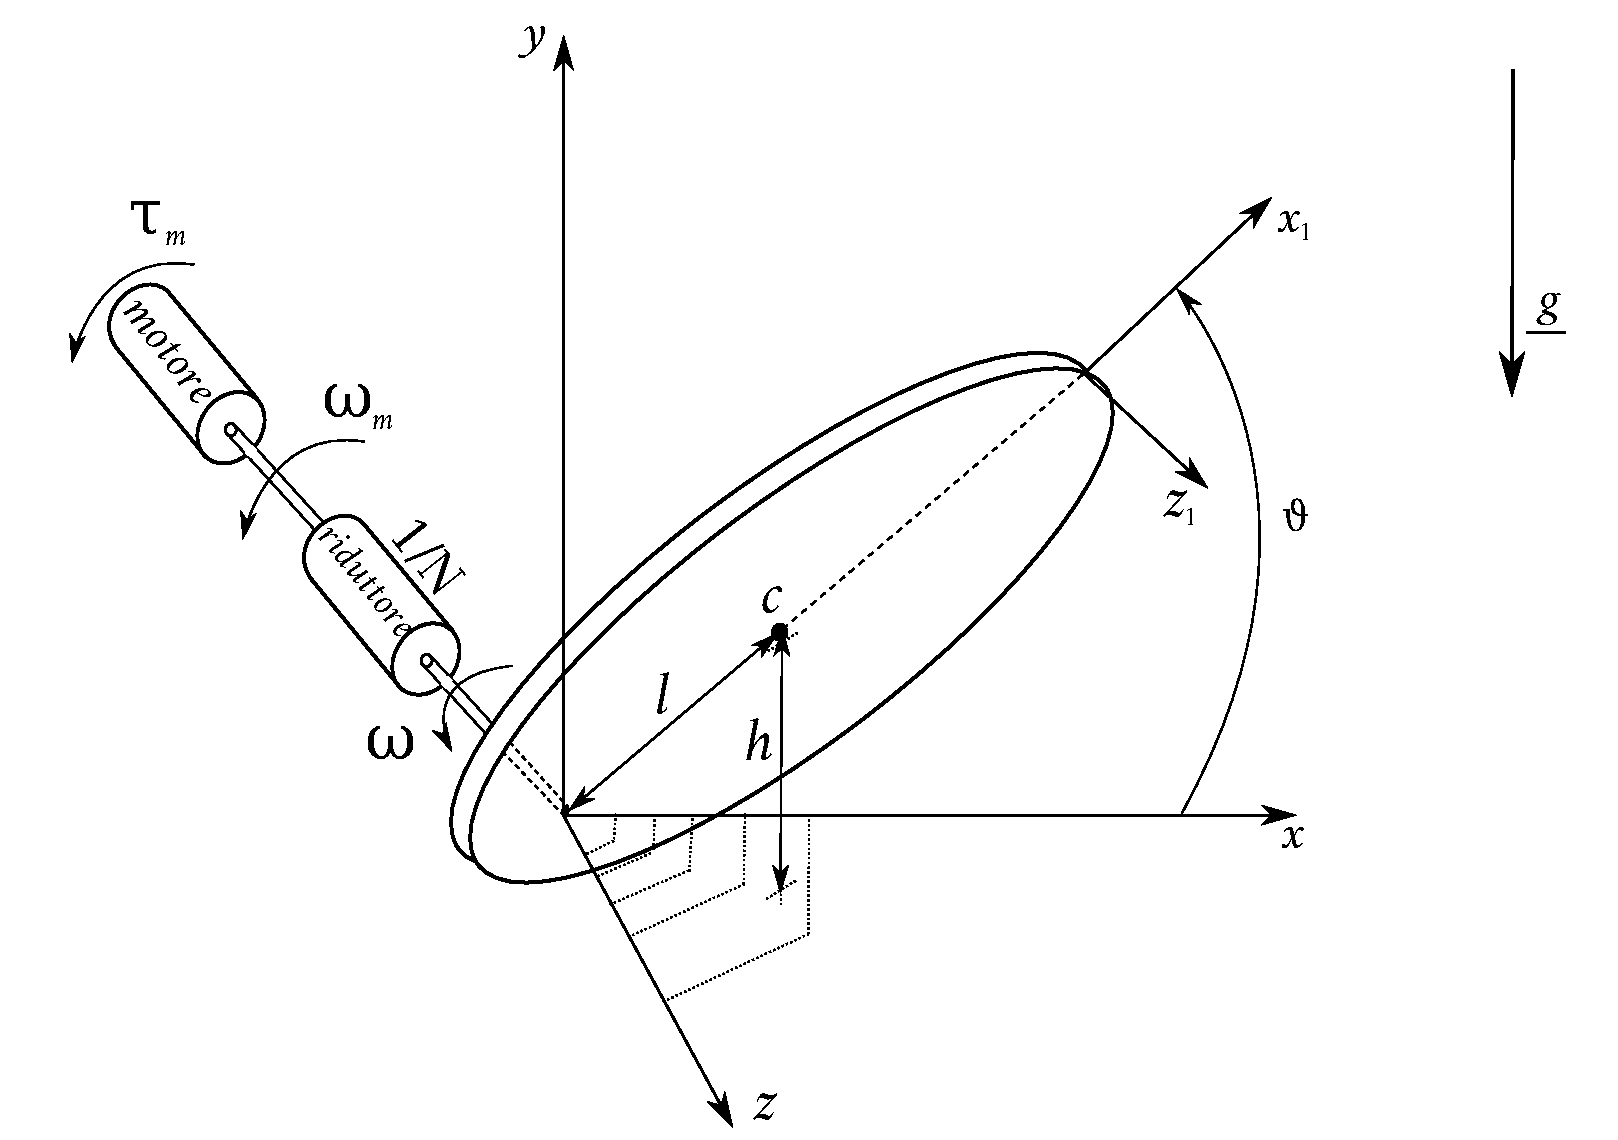
\includegraphics[scale=0.4]{pendolo.pdf}
	\caption{Pendolo motorizzato in gravità.}
\end{center}

Supponendo che il rapporto di riduzione sia $1/N$ otteniamo, 
\begin{equation}
	\begin{cases}
		\omega_m = N\omega = \dot{\vartheta}_m = N \dot{\vartheta} \\
		\tau_m \dot{\vartheta}_m = \tau \dot{\vartheta} \; \rightarrow \; \tau = \tau_m \frac{\dot{\vartheta}_m}{\dot{\vartheta}} = N \tau_m
	\end{cases}
\end{equation}
dove con $\tau$ indichiamo le forze non conservative, e pertanto scriviamo
\begin{equation*}
	\underline{\omega}_{\,l} = 
	\begin{bmatrix}
		0 \\ 0 \\ \dot{\vartheta}
	\end{bmatrix}
	\qquad I_l = 
	\begin{bmatrix}
		I_{xx} & -I_{xy} & -I_{xz} \\
		-I_{xy} & I_{yy} & -I_{yz} \\
		-I_{xz} & -I_{yz} & I_{zz} \\
	\end{bmatrix}
	\qquad \underline{p}_{\,c} =
	\begin{bmatrix}
		l \cos(\vartheta) \\ 
		l \sin(\vartheta) \\
		p_{cz} \\
	\end{bmatrix} 
	\qquad \dot{\underline{p}_{\,c}} = 
	\begin{bmatrix}
		-l \sin(\vartheta) \\
		l \cos(\vartheta) \\
		0 \\
	\end{bmatrix}
\end{equation*}
con $\underline{p}_{\,c}$ vettore identificativo del baricentro nella terna di riferimento e $p_{cz}$ costante.

\subsubsection{1. Calcoliamo l'energia cinetica del sistema:}
\paragraph{}
Per calcolare l'energia cinetica complessiva, sommiamo quella del motoriduttore $T_m$ con quella del link $T_l$. Iniziamo con la prima,
\begin{equation}
	T_m = \frac{1}{2} I_m \dot{\vartheta}_m^2 = \frac{1}{2}I_m N^2 \dot{\vartheta}^2
\end{equation}

per $T_l$ consideriamo la $(C.34)$, ovvero, il moto di traslazione del centro di massa a cui si somma una rotazione attorno al centro di massa e otteniamo,
\begin{equation}
	T_l = \frac{1}{2} m \dot{\underline{p}}_{\,c}^T \dot{\underline{p}}_{\,c} + \frac{1}{2} \underline{\omega}_{\,l}^T I_l \underline{\omega}_{\,l}
\end{equation}
e quindi, l'energia cinetica del sistema complessivo $T = T_m + T_l$ è
\begin{equation*}
	T = \frac{1}{2} \Biggl( N^2 I_m \dot{\vartheta}^2 + 
	\begin{bmatrix}
		0 & 0 & \dot{\vartheta}
	\end{bmatrix}
	\cdot
	\begin{bmatrix}
		I_{xx} & -I_{xy} & -I_{xz} \\
		-I_{xy} & I_{yy} & -I_{yz} \\
		-I_{xz} & -I_{yz} & I_{zz} \\
	\end{bmatrix}
	\cdot
	\begin{bmatrix}
		0 \\
		0 \\
		\dot{\vartheta} \\
	\end{bmatrix}
	+ m l^2
	\begin{bmatrix}
		-\sin(\vartheta) & 
		\cos(\vartheta) &
		0
	\end{bmatrix}
	\begin{bmatrix}
		- \sin(\vartheta) \\
		\cos(\theta) \\
		0 \\
	\end{bmatrix}
	\dot{\vartheta}^2
	\Biggr)
\end{equation*}
e quindi, otteniamo
\begin{equation}
	T = \frac{1}{2}\underbrace{(N^2 I_m + I_{zz} + ml^2)}_{I} \dot{\vartheta}^2 = \frac{1}{2} I \dot{\vartheta}^2
\end{equation}
dove con $I$ indichiamo il momento di inerzia totale del sistema, ridotto all'asse $z$ del pendolo.
\subsubsection{2. Calcoliamo l'energia potenziale del sistema:}
\paragraph{}
L'energia potenziale di un corpo rigido soggetto all'accelerazione di gravità $\underline{g}$, vale $U = mgh$, dove $m$ è la massa del corpo, $g$ è il modulo dell'accelerazione di gravità e $h$ è la quota del baricentro rispetto al riferimento scelto come zero per l'energia potenziale. Noi scegliamo la quota dell'origine $O$ come zero per l'energia potenziale, ovvero il piano $xz$.

Anche in questo caso dovremmo fare lo stesso discorso dell'energia cinetica, ovvero dovremmo avere $U = U_l + U_m$ ma l'energia potenziale $U_m$ è nulla per la scelta dello zero per l'energia potenziale. Otteniamo quindi
\begin{equation}
	U = mg\underbrace{l \sin(\vartheta)}_{h}
\end{equation}

\subsubsection{3. Calcoliamo la lagrangiana:}
La lagrangiana $\mathcal{L} = T - U$, scegliendo $\vartheta$ come coordinata generalizzata, risulta,
\begin{equation}
	\mathcal{L} = \frac{1}{2} I \dot{\vartheta}^2 - mgl \sin(\vartheta)
\end{equation}

\subsubsection{4. Equazioni del moto:}
Per calcolarci le equazioni del moto, ovvero la componente delle forze attive non conservative $Q = N \tau_m$, eseguiamo le derivate,
\begin{eqnarray}
	\frac{d}{dt} \Biggl( \frac{\partial \mathcal{L}}{\partial \dot{\vartheta}} \Biggr) = \frac{d}{dt} \Biggl( I\dot{\vartheta} \Biggr) = I \ddot{\vartheta} \\
	\frac{\partial \mathcal{L}}{\partial \vartheta} = -mg l \cos(\vartheta)
\end{eqnarray}
e otteniamo
\begin{equation}
	\frac{d}{dt} \Biggl( \frac{\partial \mathcal{L}}{\partial \dot{\vartheta}} \Biggr) - \frac{\partial \mathcal{L}}{\partial \vartheta} = I \ddot{\vartheta} + mgl \cos(\vartheta) = N\tau_m = Q
\end{equation}

\section{Metodo sistematico Lagrangiano}
Adesso, vogliamo applicare la \emph{formulazione di Lagrange} ad un robot a $n$ giunti, e chiaramente procederemo come nell'esempio del pendolo, esplicitando l'energia cinetica, l'energia potenziale e infine le equazioni del moto. 

\subsection{Energia cinetica}
Consideriamo un manipolatore con $n$ bracci rigidi, l'energia cinetica totale è data dalla somma dei contributi relativi al moto di ogni braccio e dei contributi relativi al moto degli attuatori ai giunti:
\begin{equation}
	T = \sum_{i = 1} ^{n} (T_{l_i} + T_{m_i})
\end{equation} 
in cui $T_{l_i}$ denota l'energia cinetica del braccio $i$ e $T_{m_i}$ denota l'energia cinetica del motore che aziona il giunto $i$.

\subsubsection{$\bullet$ Energia cinetica dei $link$:}
Facciamo l'ipotesi semplificatrice che ogni giunto $i$ rotoidale o prismatico, sia attuato da un singolo motoriduttore con statore solidale al link $i-1$. Quindi, il link $i$ collega il giunto $i$ al giunto $i+1$ e ad esso vi sarà attaccato anche il motore che muove il giunto $i+1$ con statore $i+1$ solidale al link $i$. Con riferimento alla figura,
\begin{center}
	\includegraphics[scale=0.40]{caratterizzazioneCinematica.pdf}
	\caption{Caratterizzazione cinematica del braccio $i$ ai fini della formulazione di Lagrange.}
\end{center}
definiamo,
\begin{itemize}
	\item $\underline{p}_{\,l_i} := $ vettore posizione del centro di massa del corpo rigido formato dal $link_i + statore_{i+1}$.
	\item $\dot{\underline{p}_{\,l_i}} := $ velocità del centro di massa.
	\item $\underline{\omega}_{\,i} := $ velocità angolare del $link_i$.
	\item $\underline{p}_{\,i}^* := $ punto generico appartenente al volume del $link$.
	\item $\underline{r}_{\,i} := $ vettore posizione del generico punto $\underline{p}_{\,i}^*$ rispetto a $\underline{p}_{\,l_i}$.
	\item $z_i$ e $z_{i+1}$ sono gli assi rispettivamente del giunto $i$ e del giunto $i+1$.
\end{itemize}

\paragraph{}
L'energia cinetica della particella di massa $\rho dV$ risulta
\begin{equation}
	dT = \frac{1}{2} \dot{\underline{p}}_{\,i}^{*^T}  \dot{\underline{p}}_{\,i}^* \rho dV
\end{equation}
pertanto, l'energia cinetica del braccio $i$ risulta
\begin{equation}
	T_{l_i} = \frac{1}{2} \int_{V_{l_i}} \dot{\underline{p}}_{\,i}^{*^T}  \dot{\underline{p}}_{\,i}^* \rho dV
\end{equation}
con $V_{l_i}$ il volume del braccio $i$. Considerando il vettore posizione $\underline{p}_{\,i}^*$ della particella elementare e il vettore posizione $\underline{p}_{\,l_i}$ del baricentro del braccio, entrambi riferiti alla terna base si ha
\begin{equation}
	\underline{r}_{\, i} = 
	\begin{bmatrix}
		r_x & r_y & r_z
	\end{bmatrix}^T 	
	= \underline{p}_{\,i}^* - \underline{p}_{\,l_i}
\end{equation}
con 
\begin{equation}
	\underline{p}_{\,l_i} = \frac{1}{\int_{V_{l_i}}\rho dV} \int_{V_{l_i}} \underline{p}_{\,i}^* \rho dV
\end{equation}
dove $\int_{V_{l_i}}\rho dV = m_{l_i}$ è la massa del braccio. A questo punto esprimiamo $\underline{p}_{\,i}^*$ applicando la formula fondamentale dei moti rigidi,
\begin{equation}
	\underline{p}_{\,i}^* = \dot{\underline{p}_{\,l_i}} + \underline{\omega}_{\,i} \times \underline{r}_{\,i} = \dot{\underline{p}_{\,l_i}} + S(\underline{\omega}_{\,i})\underline{r}_{\,i}
\end{equation}
e inoltre, si ha
\begin{align*}
	\underline{p}_{\,i}^{*^T} \underline{p}_{\,i}^* = \Bigl( \dot{\underline{p}}_{\,l_i}^T + \underline{r}_{\,i}^T S^T(\underline{\omega}_{\,i})\Bigr) \Bigl(\dot{\underline{p}}_{\,l_i} + S(\underline{\omega}_{\,i})\underline{r}_{\,i} \Bigr) =\\
	= \dot{\underline{p}}_{\,l_i}^T \underline{\dot{p}}_{\,l_i} + 2\dot{\underline{p}}_{\,l_i}^T S(\underline{\omega}_{\,i}) \underline{r}_{\,i} + \underbrace{\underline{r}_{\,i}^T S^T(\underline{\omega}_{\,i})S(\underline{\omega}_{\,i}) \underline{r}_{\,i}}_{\underline{\omega}_{\,i}^T S^T(\underline{r}_{\,i})S(\underline{r}_{\,i})\underline{\omega}_{\,i}}
\end{align*}
dove $\underline{\omega}_{\,i}$ indica la velocità angolare del braccio.

Riscrivendo la $(8.17)$ considerando la $(8.20)$ otteniamo,
\begin{align*}
	T_{l_i} = \int_{V_{l_i}} dT = \frac{1}{2} \int_{V_{l_i}} \Bigl[ \underline{\dot{p}}_{\,l_i}^T \underline{\dot{p}}_{\,l_i} + \underline{\omega}_{\,i}^T S^T(\underline{r}_{\,i}) S(\underline{r}_{\,i})\underline{\omega}_{\,i} + 2 \dot{\underline{p}}_{\,l_i}^T S(\underline{\omega}_{\,i})\underline{r}_{\,i} \Bigr] \rho dV = \\
	= \underbrace{\frac{1}{2} \underline{\dot{p}}_{\,l_i}^T \underline{\dot{p}}_{\,l_i} \int_{V_{l_i}} \rho dV}_{traslazione} + \underbrace{\frac{1}{2} \underline{\omega}_{\,i}^T \Biggl[ \int_{V_{l_i}} S^T(\underline{r}_{\,i})S(\underline{r}_{\,i}) \rho dV \Biggr] \underline{\omega}_{\,i}}_{rotazione} + \underbrace{\frac{1}{2} 2 \underline{\dot{p}}_{\,l_i}^T S(\underline{\omega}_{\,i}) \int_{V_{l_i}} \underline{r}_{\,i} \, \rho dV}_{= 0}
\end{align*}
e adesso analizziamo il termine di rotazione, 
\begin{align*}
	\int_{V_{l_i}} S^T(\underline{r}_{\,i})S(\underline{r}_{\,i}) \rho dV = 
	\int_{V_{l_i}}
	\underbrace{
	\begin{bmatrix}
		0 & r_z & -r_y \\
		-r_z & 0 & r_x \\
		r_y & -r_x & 0 \\
	\end{bmatrix}
	}_{S^T(\underline{r}_{\,i})}
	\cdot
	\underbrace{
	\begin{bmatrix}
		0 & -r_z & r_y \\
		r_z & 0 & -r_x \\
		-r_y & r_x & 0 \\
	\end{bmatrix}
	}_{S(\underline{r}_i)}
	\rho dV
\end{align*}
e portando l'integrale dentro la matrice otteniamo,
\begin{equation}
	\begin{bmatrix}
		\int_{V_{l_i}} (r_y^2 + r_z^2) & \int_{V_{l_i}} - r_x r_y & \int_{V_{l_i}} -r_x r_z \\
		\int_{V_{l_i}} -r_x r_y & \int_{V_{l_i}} (r_x^2 + r_z^2) & \int_{V_{l_i}} -r_y r_z \\
		\int_{V_{l_i}} -r_x r_z & \int_{V_{l_i}} -r_y r_z & \int_{V_{l_i}} (r_x^2 + r_y^2) \\
	\end{bmatrix}
	= I_{l_i}
\end{equation}
ovvero, $I_{l_i}$ è il \emph{tensore di inerzia} del link $i$ relativo al suo baricentro espresso in terna base. Notiamo che se la terna solidale al braccio $i$ coincide con la terna centrale di inerzia, i momenti centrifughi sono nulli e il tensore diventa una matrice diagonale.

Quindi, l'energia cinetica relativa al link $i$ è
\begin{equation}
	T_{l_i} = \underbrace{\frac{1}{2} m_{l_i} \underline{\dot{p}}_{\,l_i}^T \underline{\dot{p}}_{\,l_i}}_{traslazione} + \underbrace{\frac{1}{2} \underline{\omega}_{\,i}^T I_{l_i} \underline{\omega}_{\,i}}_{rotazione}
\end{equation}

\paragraph{}
Per scrivere le equazioni di Lagrange, visto che è una meccanica scalare, dobbiamo trovare un'espressione in cui siano esplicitate le coordinate generalizzate (quindi le coordinate di giunto) $\underline{q}$ e $\dot{\underline{q}}$. Pertanto, per esprimere la $(8.22)$, associamo a $\dot{\underline{p}}_{\,l_i}$ uno Jacobiano di traslazione $J_P^{(l_i)} \in \mathbb{R}^{3 \times n}$ e associamo a $\underline{\omega}_{\,i}$ uno Jacobiano di rotazione $J_O^{(l_i)} \in \mathbb{R}^{3 \times n}$, quindi otteniamo
\begin{equation}
	\begin{cases}
		\dot{\underline{p}}_{\,l_i} = J_P^{(l_i)} \underline{\dot{q}} = J_{P1}^{(l_i)} \dot{q}_1 + \cdots + J_{Pi}^{(l_i)} \dot{q}_i \\
		\underline{\omega}_{\,i} = J_O^{(l_i)} \underline{\dot{q}} = J_{O1}^{(l_i)} \dot{q}_1 + \cdots + J_{Oi}^{(l_i)} \dot{q}_i \\
	\end{cases}
\end{equation}
vengono evidenziati i contributi delle colonne degli Jacobiani relativi alle velocità dei giunti che precedono il braccio $i$ in esame, quindi gli Jacobiani da considerare sono, 
\begin{align}
	J_P^{(l_i)} = 
	\begin{bmatrix}
		J_{P1}^{(l_i)} & \cdots & J_{Pi}^{(l_i)} & 0 & \cdots & 0
	\end{bmatrix} \\
	J_O^{(l_i)} = 
	\begin{bmatrix}
		J_{O1}^{(l_i)} & \cdots & J_{Oi}^{(l_i)} & 0 & \cdots & 0
	\end{bmatrix} 
\end{align} 
e possiamo calcolare questi elementi per $j \leq i$ come segue,
\begin{align}
	J_{Pj}^{(l_i)} =
	\begin{cases}
		\underline{k}_{j-1} \qquad\qquad \qquad\qquad \text{prismatico} \\
		\underline{k}_{j-1} \times (\underline{p}_{\,l_i} - \underline{O}_{\,j-1}) \qquad \text{rotoidale}
	\end{cases}\\
	J_{Oj}^{(l_i)} = 
	\begin{cases}
		0 \qquad\qquad  \text{prismatico} \\
		\underline{k}_{j-1} \qquad\qquad \text{rotoidale}
	\end{cases}
\end{align}
dove $\underline{O}_{\,j-1}$ è il vettore posizione dell'origine e $k_{\,j-1}$ è il versore dell'asse $z$ della terna $j-1$.

Pertanto, riscrivendo l'energia cinetica del braccio $i$ della $(8.22)$ risulta
\begin{equation}
	T_{l_i} = \frac{1}{2} \underline{\dot{q}}^T \Biggl[ m_{l_i} J_P^{(l_i)^T} J_P^{(l_i)} + J_O^{(l_i)^T} I_{l_i} J_O^{(l_i)} \Biggr]\underline{\dot{q}}
\end{equation}

\subsubsection{$\bullet$ Energia cinetica dei motori:}
Per calcolare il contributo di energia cinetica relativo al motore del giunto $i$, si procede in maniera analoga a quanto visto prima. Considerando il caso tipico di motori elettrici rotanti che possono azionare sia giunti rotoidali che prismatici e supponiamo che il contributo dello statore è incluso in quello relativo al braccio su cui tale motore è situato e quindi calcoliamo solo il contributo del rotore.

\begin{center}
	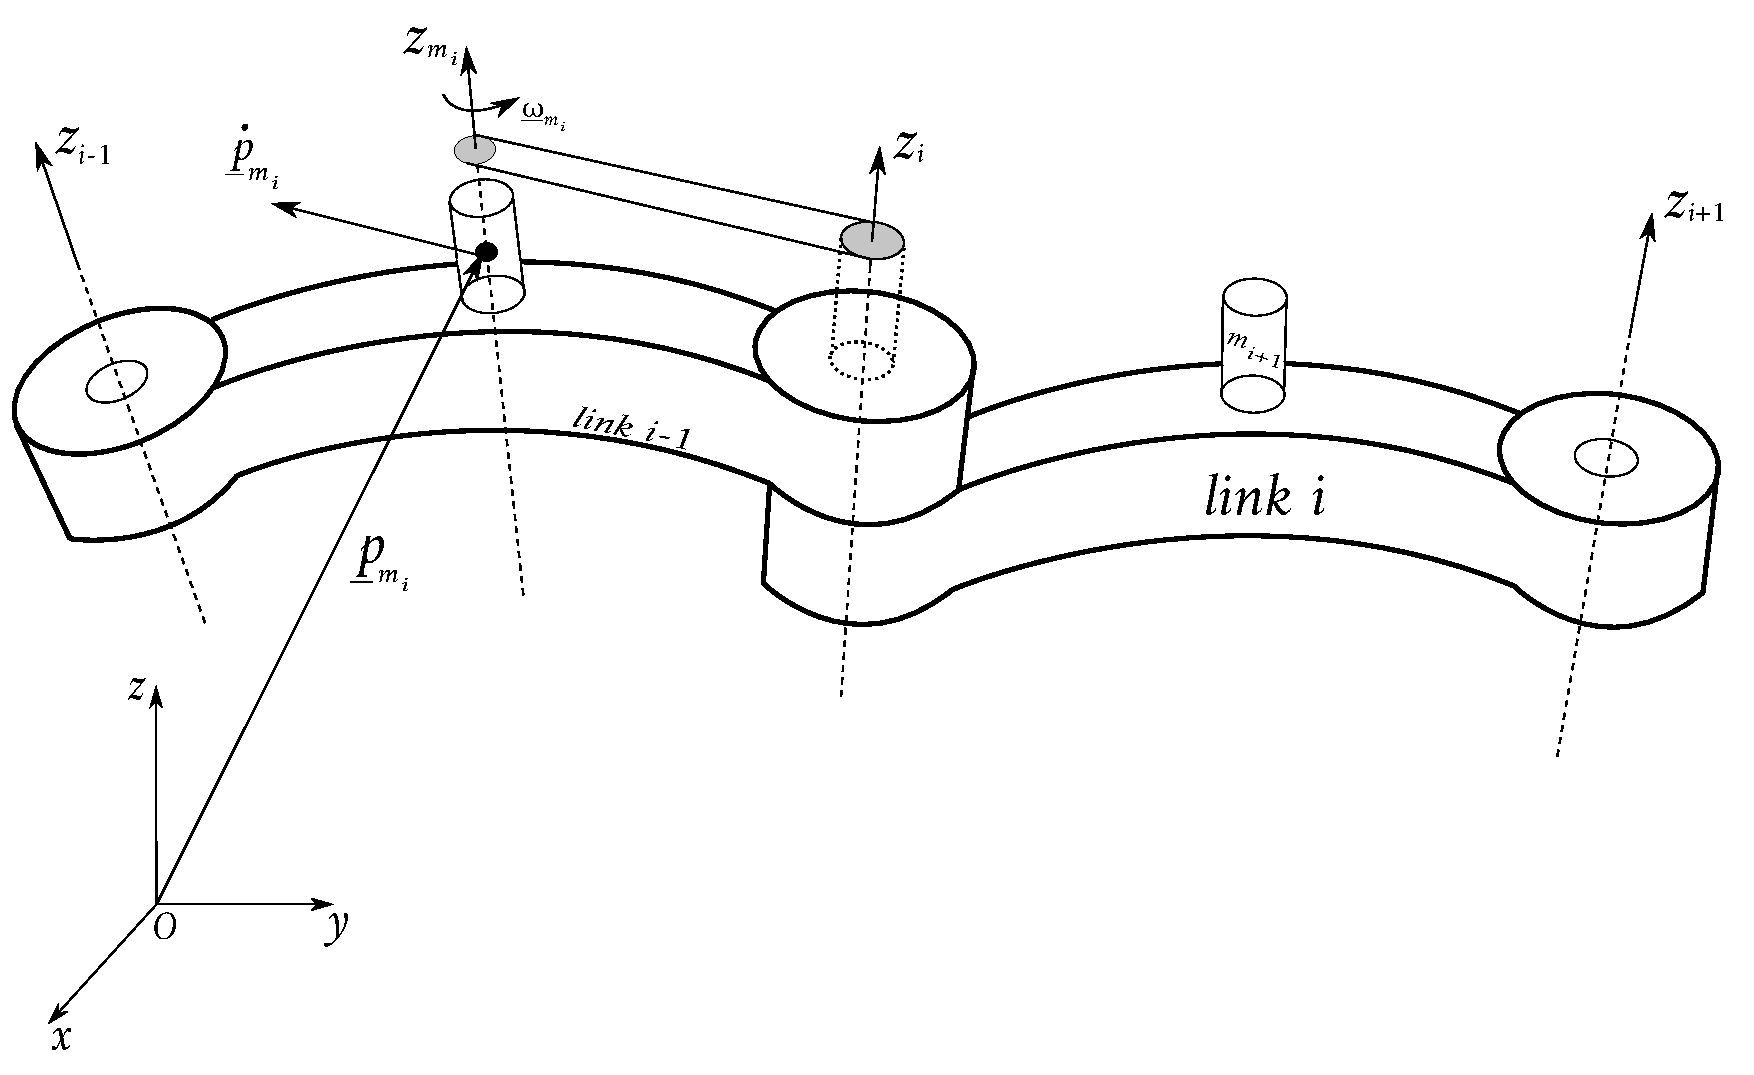
\includegraphics[scale=0.43]{caratterizzazioneMotore.pdf}
	\caption{Caratterizzazione cinematica del motore $i$ posto nel link $i-1$.}
\end{center}

Il motore del giunto $i$ si ritiene collocato sul braccio $i-1$, si suppone che non vi siano moti indotti, ovvero il motore del giunto non aziona il moto di altri giunti e pertanto la matrice di trasmissione è diagonale. L'energia cinetica del rotore $i$ può scriversi come
\begin{equation}
	T_{m_i} = \frac{1}{2} m_{m_i} \dot{\underline{p}}_{\,m_i}^T \dot{\underline{p}}_{\,m_i} + \frac{1}{2} \underline{\omega}_{\,m_i}^T I_{m_i} \underline{\omega}_{\,m_i}
\end{equation}
con $m_{m_i}$ massa del rotore, $\underline{\dot{p}}_{\,m_i}$ velocità lineare del baricentro del rotore, $I_{m_i}$ tensore di inerzia del rotore relativo al baricentro, e $\underline{\omega}_{\,m_i}$ velocità angolare del rotore. 

Notiamo inoltre che se il rapporto di riduzione tra giunto $i$ (prismatico o rotoidale) e il motoriduttore è $1/N_i$, allora otteniamo,
\begin{equation}
	\dot{\vartheta}_i = N_i \dot{\vartheta}_{m_i} \qquad \dot{d}_i = N_i \dot{\vartheta}_{m_i}
\end{equation} 
con $\vartheta_{m_i}$ posizione angolare del rotore.

\paragraph{}
L'energia cinetica $T_{m_i}$ del rotore $i$ appena trovata deve essere espressa attraverso le coordinate generalizzate, per fare ciò, procediamo in maniera analoga all'energia cinetica dei link. Infatti, associamo
\begin{equation}
	\begin{cases}
		\dot{\underline{p}}_{\,m_i} = J_P^{(m_i)} \underline{\dot{q}} \\
		\underline{\omega}_{\,m_i} = J_O^{(m_i)} \underline{\dot{q}}
	\end{cases}
\end{equation}
con $J_P^{(m_i)}$ Jacobiano di traslazione del motore e $J_O^{(m_i)}$ jacobiano di orientazione del motore, così definiti
\begin{align}
	J_P^{(m_i)} = 
	\begin{bmatrix}
		J_{P,1}^{(m_i)} & \cdots & J_{P,i-1}^{(m_i)} & 0 & \cdots & 0
	\end{bmatrix} \\
	J_O^{(m_i)} = 
	\begin{bmatrix}
		J_{O,1}^{(m_i)} & \cdots & J_{O,i-1}^{(m_i)} & 0 & \cdots & 0
	\end{bmatrix} 
\end{align}
e notiamo che $J_{Pi}^{m_i} = 0$ perchè il baricentro del rotore è posizionato sull'asse di rotazione del rotore. Calcoliamo gli elementi delle matrici,
\begin{align}
	J_{Pj}^{(m_i)} =
	\begin{cases}
		\underline{k}_{j-1} \qquad\qquad \qquad\qquad \text{prismatico} \\
		\underline{k}_{j-1} \times (\underline{p}_{\,m_i} - \underline{O}_{\,j-1}) \qquad \text{rotoidale}
	\end{cases}\\
	J_{Oj}^{(m_i)} = 
	\begin{cases}
		J_{Oj}^{(l_i)} \qquad\qquad  j = 1,\cdots,i-1 \\
		k_i z_{m_i} \qquad\qquad j = i
	\end{cases}
\end{align}
con $k_i$ rapporto di trasmissione meccanica (come può essere $1/N_i$), $z_{m_i}$ versore dell'asse di rotazione del rotore, $J_{Oj}^{(l_i)}$ Jacobiano di orientazione del link $i$ e $\underline{O}_{\,j-1}$ vettore posizione dell'origine della terna relativa al giunto $j-1$.

\paragraph{}
Quindi la $(8.29)$ si riscrive,
\begin{equation}
	T_{m_i} = \frac{1}{2} \underline{\dot{q}} \Biggl[ m_{m_i} J_P^{(m_i)^T} J_P^{(m_i)} + J_O^{(m_i)^T} I_{m_i} J_O^{(m_i)} \Biggr]\underline{\dot{q}}
\end{equation}

\subparagraph{Nota sui tensori:}
I tensori $I_{l_i}$ e $I_{m_i}$ della $(8.28)$ e della $(8.36)$ si possono scrivere usando i tensori visti rispetto alla terna solidale al link $l_i$ e motore $m_i$,
\begin{equation}
	I_{l_i} = R_i I_{l_i}^i R_i^T \qquad I_{m_i} = R_i I_{m_i}^i R_i^T
\end{equation}
con $R_i$ matrice di rotazione dalla terna solidale al braccio $i$ alla terna base, pertanto i tensori $I_{l_i}$ e $I_{m_i}$ sono tensori visti dalla terna base.

\subsubsection{$\bullet$ Energia cinetica totale:}
Andiamo a scrivere la $(8.15)$ usando la $(8.28)$ e $8.36$,
\begin{equation}
	T = \frac{1}{2} \underline{\dot{q}}^T \sum_{i = 1}^n \underbrace{\Biggl[ m_{l_i} J_P^{(l_i)^T} J_P^{(l_i)} + J_O^{(l_i)^T} I_{l_i} J_O^{(l_i)} + m_{m_i} J_P^{(m_i)^T} J_P^{(m_i)} + J_O^{(m_i)^T} I_{m_i} J_O^{(m_i)} \Biggr]}_{B(\underline{q})} \underline{\dot{q}}
\end{equation}
il termine nelle parentesi quadre rappresenta la \emph{matrice di inerzia} $B(\underline{q}) \in \mathbb{R}^{n \times n}$ che risulta \emph{simmetrica}, \emph{definita positiva} e \emph{dipendente dalla configurazione in generale}.

\subsection{Energia potenziale}
Per l'energia potenziale, il discorso è analogo a quanto visto per l'energia cinetica. Ovvero, l'energia potenziale totale del sistema è data dalla somma dei contributi relativi ad ogni braccio e dei contributi relativi ai rotori dei motori dei giunti,
\begin{equation}
	U = \sum_{i=1}^n (U_{l_i} + U_{m_i})
\end{equation}

Per il contributo del link, utilizziamo la figura 8.2 e otteniamo,
\begin{equation}
	U_{l_i} = - \int_{V_{l_i}} \underline{g}^T \underline{p}_{\,i}^* \rho dV = -m_{l_i} \underline{g}^T \underline{p}_{\,l_i}
\end{equation}
in cui $\underline{g}$ è il vettore accelerazione gravitazionale riferito alla terna base.

Per quanto riguarda il contributo del rotore $i$, con riferimento alla figura 8.3 si ha,
\begin{equation}
	U_{m_i} = - m_{m_i} \underline{g}^T \underline{p}_{\,m_i}
\end{equation}

Pertanto, riscrivendo la $(8.39)$ otteniamo,
\begin{equation}
	U = - \sum_{i=1}^n \Bigl( m_{l_i} \underline{g}^T \underline{p}_{\,l_i} + m_{m_i} \underline{g}^T \underline{p}_{\,m_i} \Bigr)
\end{equation}
e notiamo che è una funzione solo di $\underline{q}$ e non di $\underline{\dot{q}}$ perchè dipende dai vettori $\underline{p}_{\,l_i}$ e $\underline{p}_{\,m_i}$. 

\subsection{Equazioni del moto}
Tenendo conto delle espressioni $(8.38)$ e $(8.42)$ andiamo a scrivere la Lagrangiana,
\begin{equation}
	\mathcal{L}(\underline{q}, \dot{\underline{q}}) = T(\underline{q}, \dot{\underline{q}}) - U(\underline{q})
\end{equation}
a questo punto, eseguendo le varie derivate, otteniamo
\begin{equation}
	B(\underline{q})\ddot{\underline{q}} + n(\underline{q}, \underline{\dot{q}}) = \underline{Q}
\end{equation}
dove $\underline{Q}$ rappresenta il vettore delle forze attive non conservative e $n(\underline{q}, \underline{\dot{q}})$ ha la seguente forma
\begin{equation}
	n(\underline{q}, \underline{\dot{q}}) = \dot{B}(\underline{q})\dot{\underline{q}} - \frac{1}{2} \Biggl( \frac{\partial}{\partial \underline{q}} \Bigl( \dot{\underline{q}}^T B(\underline{q}) \dot{\underline{q}} \Bigr) \Biggr)^T + \Biggl( \frac{\partial U(\underline{q})}{\partial \underline{q}} \Biggr)^T 
\end{equation}
\paragraph{}
Per esplicitare le forze non conservative che compiono lavoro sui giunti del manipolatore, andiamo a definire le seguenti componenti:
\begin{itemize}
	\item \textbf{Le forze di attuazione:} rappresentate dal vettore $\underline{\tau} \in \mathbb{R}^n$.
	\item \textbf{Le forze di attrito viscoso:} $F_v \underline{\dot{q}}$ con $F_v \in \mathbb{R}^{n \times n}$ matrice dei coefficienti di attrito viscoso.
	\item \textbf{Le forze di attrito statico:} $f_s(\underline{q}, \underline{\dot{q}})$ che possiamo esplicitare come attrito \emph{coulumbiano} $f_s = F_s\, sgn(\underline{\dot{q}})$ con $F_s \in \mathbb{R}^{n \times n}$ e $sgn(\underline{\dot{q}}) \in \mathbb{R}^{n \times 1}$ le cui componenti sono date dalle funzioni segno delle velocità dei singoli giunti.
	\item \textbf{Le forze di contatto:} definite solo se l'organo terminale è in contatto con l'ambiente, allora vi è un \emph{wrench} di forza pari a $J^T(\underline{q})\underline{\gamma}$ con $\underline{\gamma}$ vettore di forza e momento esercitati dall'organo terminale del manipolatore sull'ambiente.  
\end{itemize}
e otteniamo
\begin{equation}
	\underline{Q} = \underline{\tau} - F_v \, \underline{\dot{q}} - F_s\, sgn(\underline{\dot{q}}) - J^T(\underline{q})\underline{\gamma}
\end{equation}

\paragraph{}
Le equazioni del moto $(8.44)$ possono essere riscritte nella forma matriciale compatta che rappresenta il \emph{modello dinamico nello spazio dei giunti},
\begin{equation}
	B(\underline{q})\ddot{\underline{q}} + C(\underline{q}, \underline{\dot{q}}) \underline{\dot{q}} + \underline{g}(\underline{q}) = \underline{\tau} - F_v \,\underline{\dot{q}} - F_s \, sgn(\underline{\dot{q}}) - J^T(\underline{q}) \underline{\gamma}
\end{equation}
dove:
\begin{itemize}
	\item $B(\underline{q}) \in \mathbb{R}^{n \times n}$ è la \emph{matrice di inerzia}.
	\item $C(\underline{q}, \underline{\dot{q}}) \in \mathbb{R}^{n \times n}$ è la matrice dei termini di Coriolis e centrifughi.
	\item $\underline{g}(\underline{q}) \in \mathbb{R}^n$ è il vettore delle azioni delle forze di gravità sui giunti. Si ricava nel derivare l'energia potenziale totale, $\partial U / \partial q_i = g_i(\underline{q})$.
\end{itemize}
e infine, come abbiamo già accennato, possiamo ricavare la \emph{dinamica diretta},
\begin{equation}
	\underline{\ddot{q}} = B^{-1}(\underline{q}) \Bigl[ \underline{\tau} - C(\underline{q}, \underline{\dot{q}})\underline{\dot{q}} - F_v \,\underline{\dot{q}} - F_s \, sgn(\underline{\dot{q}}) - \underline{g}(\underline{q}) - J^T(\underline{q}) \underline{\gamma} \Bigr]
\end{equation}
dove chiaramente abbiamo invertito la matrice $B(\underline{q})$, operazione possibile dato che la matrice è simmetrica e definita positiva.

\section{Proprietà del modello dinamico}
Presentiamo delle proprietà notevoli del modello dinamico ricavato nella $(8.47)$, un'importante proprietà che non approfondiamo ma che si utilizza per dimostrare la stabilità per certi algoritmi di controllo è l'anti-simmetria della matrice così definita
\begin{equation}
	N(\underline{q}, \underline{\dot{q}}) = \dot{B}(\underline{q}) - 2C(\underline{q}, \underline{\dot{q}})
\end{equation}
ovvero,
\begin{equation}
	\underline{v}^T \, N(\underline{q}, \underline{\dot{q}})\, \underline{v} = 0 \qquad \forall \underline{v} \in \mathbb{R}^{n \times 1}
\end{equation}
detto ciò, passiamo a proprietà più significative.

\subsection{Linearità dei parametri dinamici}
Una importante proprietà del modello dinamico è la \emph{linearità} rispetto ai \emph{parametri dinamici} caratteristici die bracci e dei rotori del manipolatore. L'obiettivo è quello di individuare questi parametri indipendenti dalla configurazione dei giunti del manipolatore, consideriamo pertanto il \emph{link} $l_i$ come corpo rigido che comprende il \emph{motore} $m_{i+1}$ come in figura
\begin{center}
	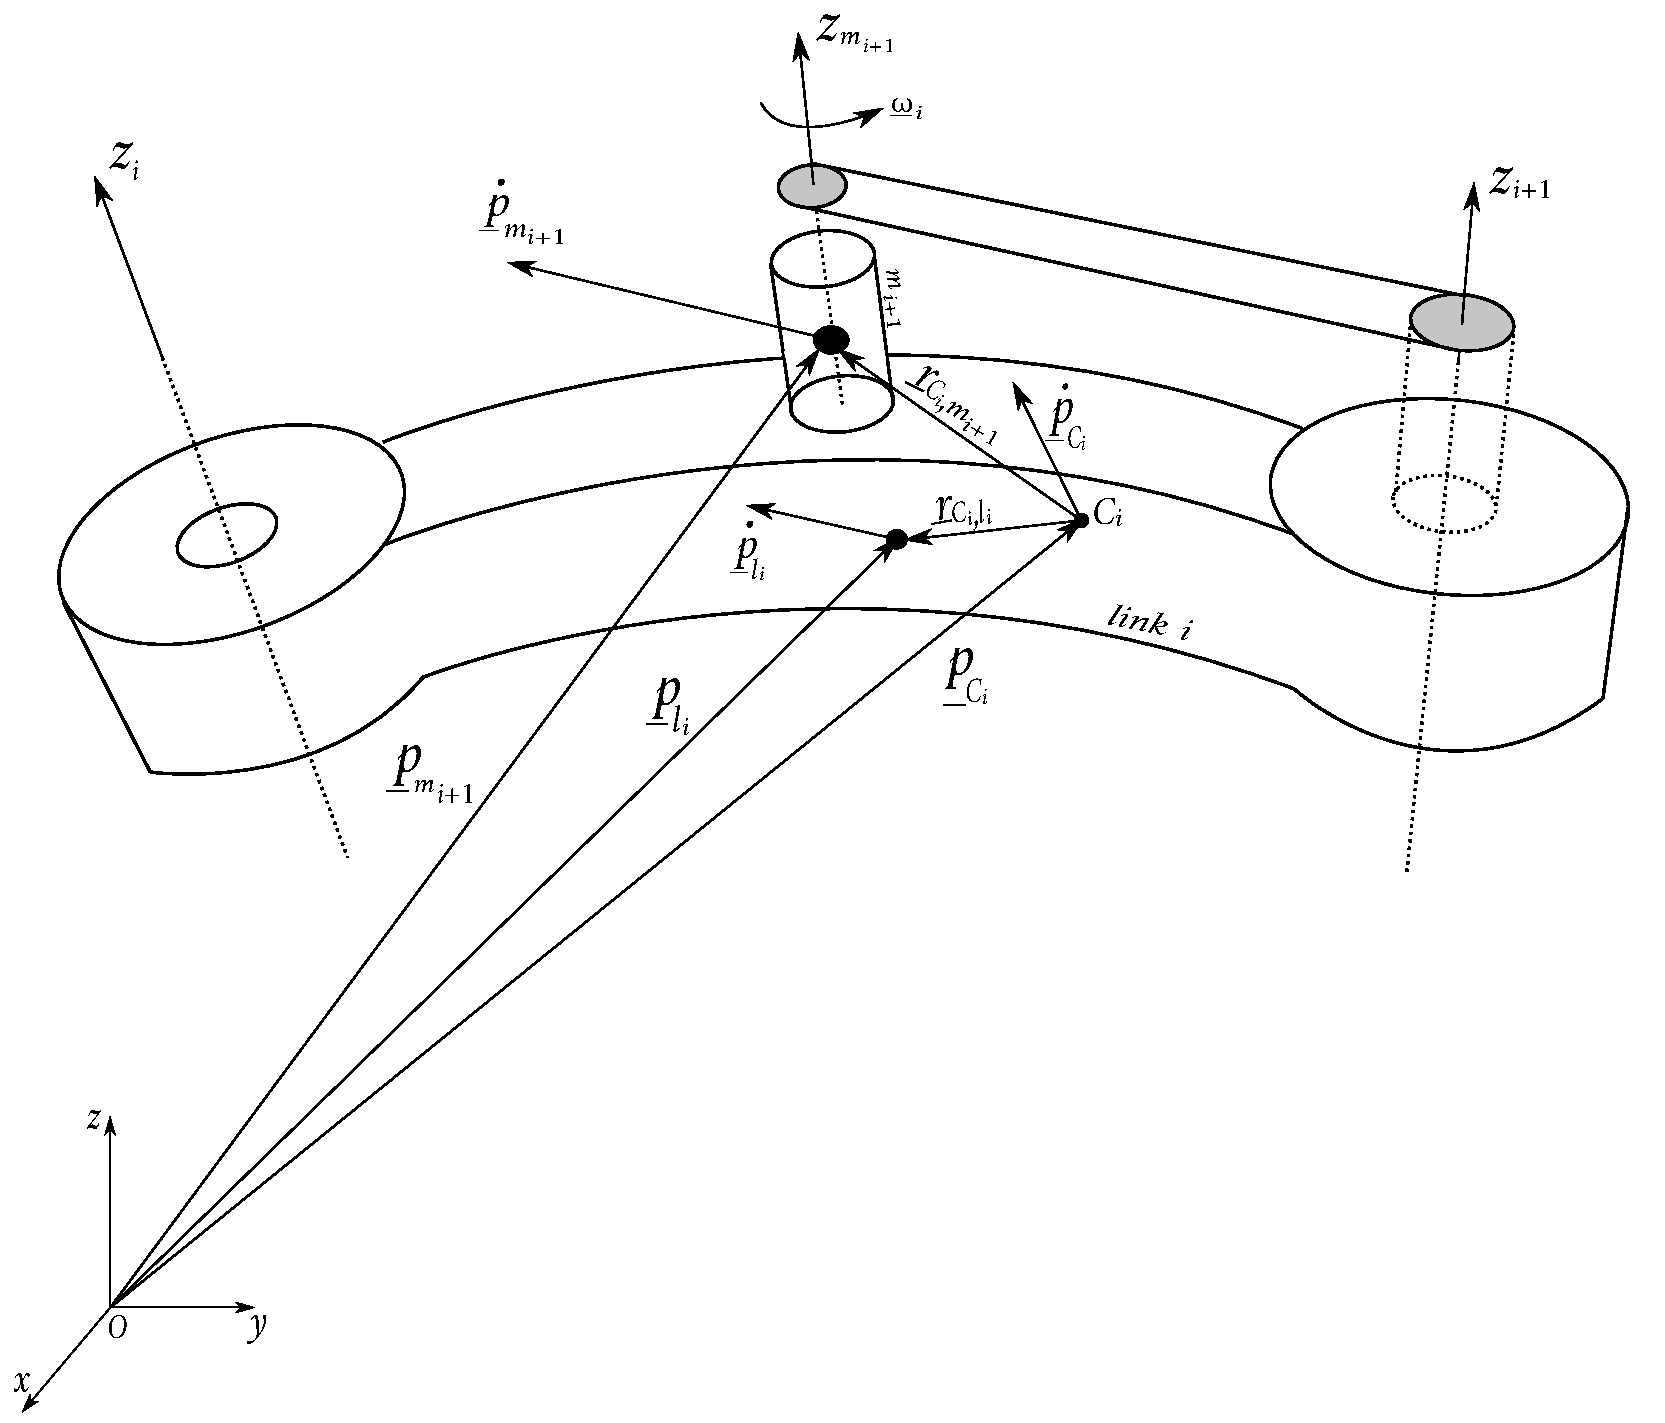
\includegraphics[scale=0.4]{linearitaProprietaDinamici.pdf}
	\caption{Caratterizzazione cinematica del \emph{link} $i$}
\end{center}
e pertanto possiamo definire il centro di massa di questo corpo rigido composto dal link e dal rotore come $C_i$, quindi utilizzando la descrizione cinematica dei rigidi otteniamo
\begin{equation}
	\begin{cases}
		\underline{r}_{\,C_i,l_i} = \underline{p}_{\,l_i} - \underline{p}_{\,C_i} \\
		\underline{r}_{\,C_i,m_{i+1}} = \underline{p}_{\,m_{i+1}} - \underline{p}_{\,C_i} 
	\end{cases}
	\qquad
	\begin{cases}
		\underline{\dot{p}}_{\,l_i} = \underline{\dot{p}}_{\,C_i} + \underline{\omega}_{\,i} \times \underline{r}_{\,C_i,l_i} \\
		\underline{\dot{p}}_{\,m_{i+1}} = \underline{\dot{p}}_{\,C_i} + \underline{\omega}_{\,i} \times \underline{r}_{\,C_i,m_{i+1}}
	\end{cases}
\end{equation}
dove $\underline{p}_{\,C_i}$ denota il vettore posizione del baricentro dell'insieme braccio + rotore.

\paragraph{}
Scriviamo l'energia cinetica del complessivo corpo rigido $i$, 
\begin{equation}
	T_i = T_{l_i} + T_{m_{i+1}}
\end{equation}
con $T_{l_i}$ pari a $(8.22)$ e $T_{m_{i+1}}$ pari a $(8.29)$ con la massa $m_{i+i}$ invece della massa $m$.

Per poter scrivere l'energia cinetica si riscrive $T_{l_i}$ e $T_{m_{i+1}}$ con le $(8.51)$ e otterremo, col teorema di Steiner, i seguenti tensori di inerzia relativi al baricentro complessivo $\underline{p}{\,C_i}$,
\begin{equation}
	\begin{cases}
		\overline{I}_{l_i} = I_{l_i} + m_{l_i} S^T(\underline{r}_{\,C_i, l_i})S(\underline{r}_{\,C_i, l_i}) \\
		\overline{I}_{m_{i+1}} = I_{m_{i+1}} + m_{m_{i+1}} S^T(\underline{r}_{\,C_i, m_{i+1}})S(\underline{r}_{\,C_i, m_{i+1}})
	\end{cases}
\end{equation}
e pertanto, esprimiamo la \emph{massa complessiva} del rigido $i$ come $m_i = m_{l_i} + m_{m_{i+1}}$ e il \emph{tensore di inerzia complessivo} come $\overline{I}_i = \overline{I}_{l_i} + \overline{I}_{m_{i+1}}$. 

\paragraph{}
Finora abbiamo espresso tutto in terna fissa, ma dato che l'obiettivo è trovare dei parametri indipendenti dalle configurazioni di giunto, andiamo ad esprimere le seguenti relazioni
\begin{equation}
	\begin{cases}
		\underline{p}_{\,C_i}^i = \underline{p}_i^i + \underline{r}_{\,i,C_i}^i \\
		\underline{\dot{p}}_{\,C_i}^i = \underline{\dot{p}}_i^i + \underline{\omega}_i^i \times \underline{r}_{\,i,C_i}^i
	\end{cases}
\end{equation}
in cui si sono espressi tutti i vettori nella terna $i$ e chiaramente $\underline{r}_{i,C_i}^i$ è fisso in tale terna e vale
\begin{equation}
	\underline{r}_{\,i,C_i}^i = 
	\begin{bmatrix}
		l_{C_ix} & l_{C_iy} & l_{C_iz}
	\end{bmatrix}^T
\end{equation}

Inoltre, il tensore di inerzia $I_{m_i}^{m_i}$ è chiaramente diagonale, otteniamo
\begin{equation}
	I_{m_{i+1}} \cdot z_{m_{i+1}} = I_{m_{i+1}zz} \cdot z_{m_{i+1}}
\end{equation}
dove, il membro di sinistra è il tensore e quello di destra è il momento di inerzia proiettato nel proprio asse di rotazione.

Riscrivendo l'energia cinetica otteniamo il tensore di inerzia rispetto all'origine della terna $i$ 
\begin{equation}
	\hat{I}_{i}^{i} = \overline{I}_{i}^i + m_i S^T(\underline{r}_{\,i, C_i}^i)S(\underline{r}_{\,i, C_i}^i)
\end{equation}
e il \emph{momento primo di inerzia}
\begin{equation}
	m_i \underline{r}_{\,i,C_i}^i = 
	\begin{bmatrix}
		m_i l_{C_ix} \\
		m_i l_{C_iy} \\
		m_i l_{C_iz} 
	\end{bmatrix}
\end{equation}
quindi scriviamo il tensore,
\begin{equation}
	\hat{I}_{i}^{i} = 
	\begin{bmatrix}
		\hat{I}_{ixx} & -\hat{I}_{ixy} & -\hat{I}_{ixz} \\
		-\hat{I}_{ixy} & \hat{I}_{iyy} & -\hat{I}_{iyz} \\
		-\hat{I}_{ixz} & -\hat{I}_{iyz} & \hat{I}_{izz}
	\end{bmatrix}
\end{equation}

Pertanto $T_i$ del corpo rigido braccio $i$ e rotore $i+1$ è lineare rispetto ai parametri dinamici seguenti:
\begin{itemize}
	\item la \emph{massa} $m_i = m_{l_i} + m_{m_{i+1}}$
	\item le tre componenti del \emph{momento primo di inerzia} $m_i \underline{r}_{\,i,C_i}^i$
	\item le sei componenti del tensore di inerzia $\hat{I}_i^i$ solidale al link
	\item il momento di inerzia del motore rispetto al proprio asse di rotazione $I_{m_izz}$
\end{itemize} 
\paragraph{}
L'energia potenziale dell'insieme braccio $i$ e rotore $i+1$ risulta
\begin{equation}
	U_i = -\underline{g}_i^T(m_i \underline{p}_i^i + m_i \underline{r}_{\,i,C_i}^i)
\end{equation}
e pertanto è lineare rispetto alla massa e alle tre componenti del momento primo di inerzia.

Quindi, infine possiamo scrivere la lagrangiana come
\begin{equation}
	\mathcal{L} = \sum_{i=1}^n \Bigl( \beta_{T_i} - \beta_{U_i} \Bigr) \underline{\pi_i}
\end{equation}
dove abbiamo evidenziato il vettore dei \emph{parametri dinamici},
\begin{equation}
	\underline{\pi_i} = 
	\begin{bmatrix}
		m_i \\ m_i l_{C_ix} \\ m_i l_{C_iy} \\ m_i l_{C_iz} \\ \hat{I}_{ixx} \\ \hat{I}_{ixy} \\ \hat{I}_{ixz} \\ \hat{I}_{iyy} \\ \hat{I}_{iyz} \\ \hat{I}_{izz} \\ I_{m_izz}
	\end{bmatrix}
	\in \mathbb{R}^{11 \times 1}
\end{equation}

I vettori $\beta_{T_i} \in \mathbb{R}_{11 \times 1}$ e $\beta_{U_i} \in \mathbb{R}_{11 \times 1}$ consentono di scrivere la lagrangiana in funzione di $\underline{\pi_i}$, inoltre anche le operazioni di derivazioni non alterano la proprietà di linearità. Pertanto la \emph{forza generalizzata} non conservativa del giunto $i$ può scriversi come
\begin{equation}
	Q_i = \sum_{j=1}^n y_{ij}^T \, \underline{\pi_j}
\end{equation}
dove 
\begin{equation}
	y_{ij} = \frac{d}{dt} \Biggl( \frac{\partial \beta_{T_j}}{\partial \dot{q}_i} \Biggr) - \frac{\partial \beta_{T_j}}{\partial q_i} + \frac{\partial \beta_{U_j}}{\partial q_i}
\end{equation}
e notiamo che le derivate parziali sono nulle per $j<i$, pertanto otteniamo la seguente espressione matriciale, esplicitando $Q_i = \tau_i$,
\begin{equation}
	\begin{bmatrix}
		\tau_1 \\
		\tau_2 \\
		\vdots \\
		\tau_n \\
	\end{bmatrix}
	= 
	\begin{bmatrix}
		y_{11}^T & y_{12}^T & \cdots & y_{1n}^T \\
		0^T & y_{22}^T & \cdots & y_{2n}^T \\
		\vdots & \vdots & \ddots & \vdots \\
		0^T & 0^T & \cdots & y_{nn}^T
	\end{bmatrix}
		\cdot
	\begin{bmatrix}
		\pi_1 \\
		\pi_2 \\
		\vdots \\
		\pi_n \\
	\end{bmatrix}
\end{equation}
e notiamo che questa espressione matriciale esprime la \textbf{linearità del modello dinamico} del manipolatore rispetto a un insieme opportuno di \textbf{parametri dinamici}.

Inoltre, è opportuno includere il coefficiente di attrito viscoso e di attrito Coulombiano tra i parametri di $\underline{\pi_i}$ arrivando a $13$ parametri per ogni giunto. Scrivendo in forma compatta,
\begin{equation}
	\underline{\tau} = Y(\underline{q}, \underline{\dot{q}}, \underline{\ddot{q}}) \underline{\pi}
\end{equation}
dove $\underline{\pi} \in \mathbb{R}^{p \times 1}$ è un vettore di $p$ parametri \emph{costanti}, con $p < 13n$ in quanto non è detto che tutti e 13 parametri di ogni giunto compaiano esplicitamente nella $(8.65)$; Si ha $Y \in \mathbb{R}^{n \times p}$ matrice che rispecchia la proprietà di linearità del modello dinamico dipendente dalle posizioni, velocità e accelerazioni dei giunti. $Y$ prende il nome di \emph{regressore}. 

\subsection{Identificazioni dei parametri dinamici}
Questa non è una proprietà vera e propria, ma riguarda il calcolo effettivo dei parametri dinamici della $(8.62)$. In effetti, il loro calcolo è parecchio laborioso anche se si usano software di calcolo.

Per ricavare stime accurate dei parametri dinamici si ricorre a tecniche di identificazione che sfruttano la proprietà di linearità $(8.65)$. Queste tecniche consentono di ricavare il vettore $\underline{\pi}$ sulla base di misure effettuate, durante l'esecuzione di opportune traiettorie di moto imposte al manipolatore, così da ricavare numericamente la matrice $Y$.

A questo punto, supponendo di aver ricavato, nell'esecuzione della traiettoria imposta al manipolatore, le misure di forza, posizioni, velocità e accelerazioni ai giunti in corrispondenza degli istanti di tempo $t_1, \cdots, t_N$, si può scrivere
\begin{equation}
	\overline{\underline{\tau}} = 
	\begin{bmatrix}
		\underline{\tau}(t_1) \\
		\vdots \\
		\underline{\tau}(t_N)
	\end{bmatrix}
	= 
	\begin{bmatrix}
		Y(t_1) \\
		\vdots \\
		Y(t_N)
	\end{bmatrix}
	\underline{\pi}
	= \overline{Y} \underline{\pi}
\end{equation}
con un numero di istanti molto alto, ovvero $Nn \gg p$.

Risolvendo la $(8.67)$ con una tecnica ai minimi quadrati, si ottiene la soluzione nella forma
\begin{equation}
	\underline{\pi} = \Bigl( \overline{Y}^{\,T} \overline{Y} \Bigr)^{-1}  \overline{Y}^{\,T} \overline{\underline{\tau}}
\end{equation}
dove $\Bigl( \overline{Y}^{\,T} \overline{Y} \Bigr)^{-1}  \overline{Y}^{\,T}$ è la matrice pseudo-inversa di sinistra di $\overline{Y}$.
\chapter{Controllo del moto}
\paragraph{}
Il problema del controllo di un manipolatore consiste nel determinare l'andamento delle forze generalizzate che gli attuatori devono applicare ai giunti in modo da garantire, con il soddisfacimento di specifiche assegnate sul transitorio e sul regime, l'esecuzione delle operazioni comandate.

Le operazioni consistono nell'esecuzione di moti assegnati al manipolatore che comprenderanno due aspetti:
\begin{itemize}
	\item moto dell'organo terminale nello \emph{spazio libero}.
	\item moto dell'organo terminale nell'interazione con \emph{l'ambiente}.
\end{itemize} 
Le tecniche di controllo possono essere,
\begin{itemize}
	\item nello \emph{\textbf{spazio dei giunti}}, dove possiamo distinguere:
	\begin{itemize}
		\item Controllo \emph{centralizzato} in cui si tiene conto degli effetti dinamici di interazione con gli altri giunti.
		\item Controllo \emph{decentralizzato} in cui il singolo giunto del manipolatore viene controllato in maniera indipendente dal moto degli altri giunti. 
	\end{itemize}
	\item e direttamente nello \emph{\textbf{spazio operativo}}.
\end{itemize}

\section{Tecniche di controllo del moto}
In generale, \emph{le caratteristiche di moto} sono specificate nello spazio operativo, le \emph{azioni di controllo} vengono esplicate in maniera diretta nello spazio dei giunti mediante le forze generalizzate sviluppate dagli attuatori. Questa caratteristica porta ad individuare due modalità di controllo illustrate di seguito.

\subsubsection{\underline{Controllo nello spazio dei giunti:}} 
Si articola in due sottoproblemi:
\begin{enumerate}
	\item Inversione della cinematica del manipolatore per la traduzione delle specifiche di moto, generate nello spazio operativo $\underline{x}_{\,d}$ (desiderata), in grandezze di riferimento espresse nello spazio dei giunti $\underline{q}_{\,d}$ (desiderata);
	\item Realizzazione di un sistema di controllo nello spazio dei giunti che deve garantire l'inseguimento dei riferimenti da parte delle grandezze controllate $\underline{q}$.
\end{enumerate}

\begin{center}
	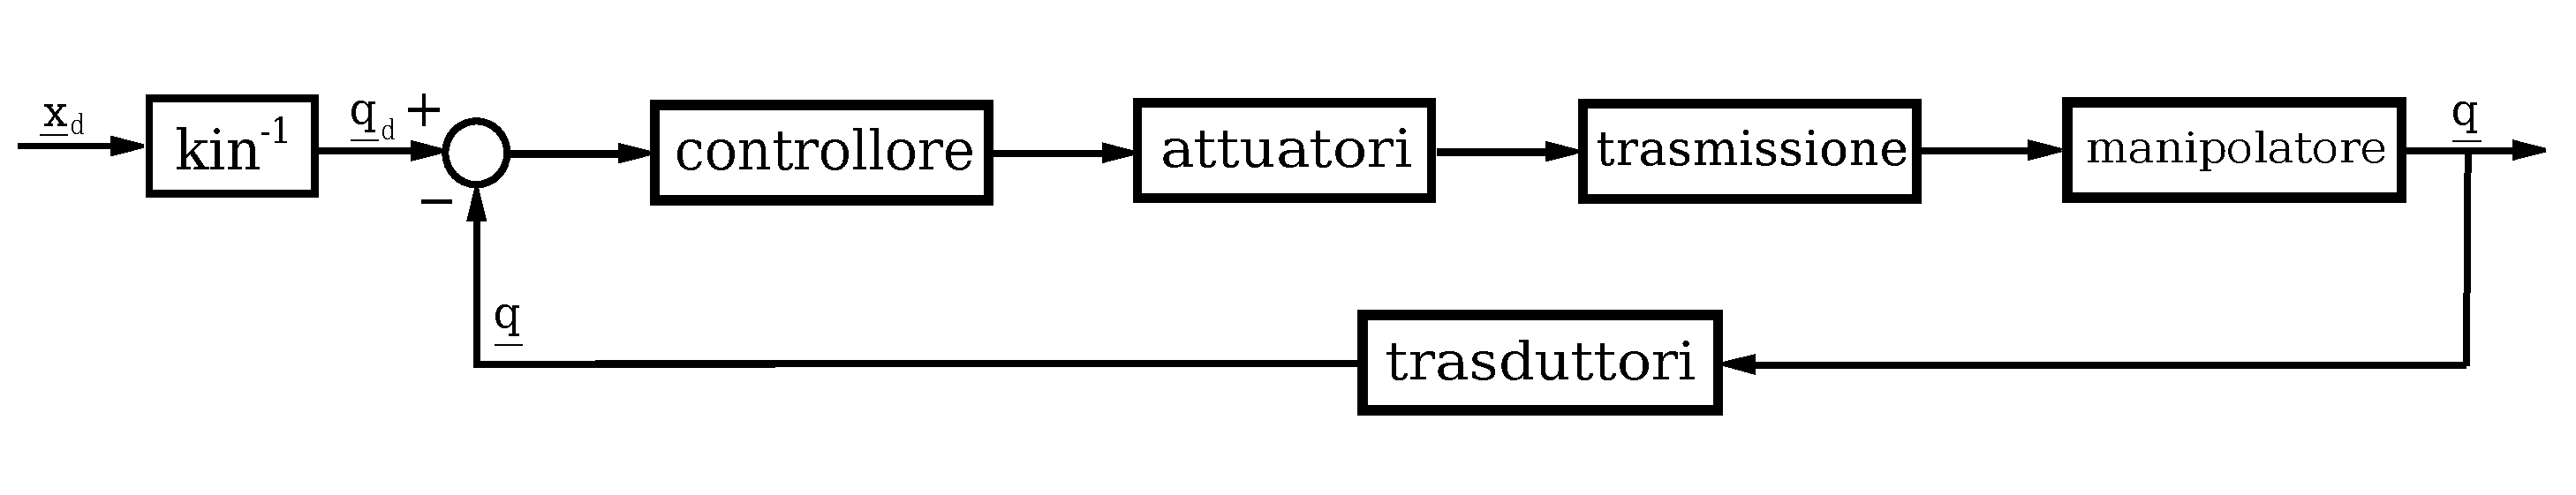
\includegraphics[scale=0.25]{schemaSpazioDeiGiunti.pdf}
	\caption{Schema di principio di controllo nello spazio dei giunti.}
\end{center}

\subsubsection{\underline{Controllo nello spazio operativo:}}
Questa soluzione segue un approccio di tipo globale che richiede una maggiore complessità algoritmica, con tale soluzione infatti, l'inversione cinematica è implicitamente assunta interna all'anello di controllo.

\begin{center}
	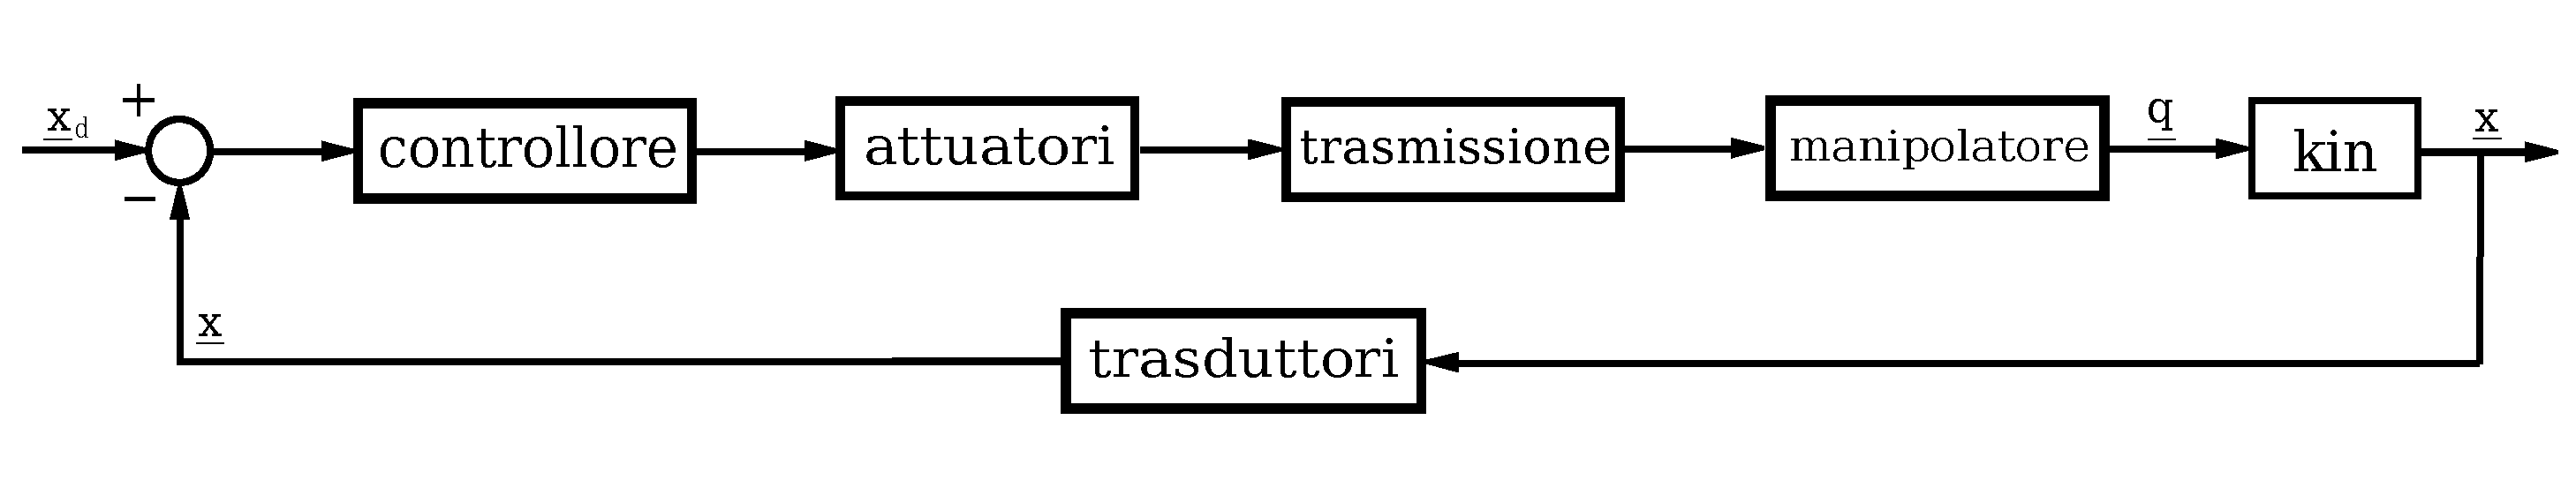
\includegraphics[scale=0.25]{schemaSpazioOperativo.pdf}
	\caption{Schema di principio di controllo nello spazio operativo.}
\end{center}

\subsubsection{\underline{Discorso qualitativo:}}
Le specifiche di moto sono usualmente prescritte nello spazio operativo e come si nota nella Figura 9.1 è pertanto necessario utilizzare un algoritmo di inversione cinematica per poter ricavare i riferimenti degli schemi di controllo operanti nello spazio dei giunti. Questa inversione presenta un carico computazionale notevole, specie se si richiede anche l'inversione della cinematica differenziale del primo e del secondo ordine (velocità e accelerazione). 

Un approccio alternativo consiste nel considerare schemi di controllo sviluppati direttamente nello spazio operativo, come illustrato nella Figura 9.2. L'impiego di tali schemi è vantaggioso quando ci poniamo il problema del controllo del manipolatore in situazioni di \emph{interazione con l'ambiente}. 

Gli schemi di controllo nello spazio operativo sono basati sul confronto diretto degli ingressi, che specificano le traiettorie nello spazio operativo, con le misure delle corrispondenti grandezze di uscita del manipolatore. Ne consegue che nel controllore devono essere presenti delle azioni che consentono di passare dallo spazio operativo, in cui è valutato l'errore di inseguimento, allo spazio dei giunti, in cui sono esplicate le forze generalizzate di controllo.

\section{Controllo Decentralizzato}
Iniziamo trattando il controllo nello spazio dei giunti, in particolare illustriamo la tecnica del controllo decentralizzato. Riscriviamo le equazioni del moto di un manipolatore completo di attuatori (motori) $(8.47)$ trascurando le forze esterne e le forze di attrito statico,
\begin{equation}
	B(\underline{q})\ddot{\underline{q}} + C(\underline{q}, \underline{\dot{q}}) \underline{\dot{q}} + \underline{g}(\underline{q}) + F_v \,\underline{\dot{q}} = \underline{\tau}   
\end{equation}

\paragraph{}
Controllare il moto di un manipolatore nello spazio libero significa determinare le $n$ componenti di forza generalizzata, (\emph{coppie per i giunti rotoidali e forze per i giunti prismatici}), che consentono di realizzare un moto $\underline{q}(t)$ tale che risulti $\underline{q}(t) = \underline{q}_{\,d}(t)$. Con $\underline{q}_{\,d}(t)$ indichiamo il vettore delle  variabili di giunto con le $n$ traiettorie di riferimento specificate per gli $n$ giunti.

\paragraph{}
Sia $\underline{q}_{\,m}$ il vettore delle variabili di posizione dei motori, sia $\underline{q}$ il vettore delle coordinate dei giunti e sia $K_r$ la matrice dei rapporti di trasmissione, otteniamo le seguenti relazioni,
\begin{equation}
	\underline{q}_{\,m} = K_r \underline{q} \qquad \qquad \underline{q} = K_r^{-1} \underline{q}_{\,m}
\end{equation}
sia $\underline{\tau}_{\,m}$ il vettore delle azioni sui motori e sia $\underline{\tau}$ il vettore delle azioni sui giunti, facciamo qualche considerazione energetica eguagliando la potenza erogata nello spazio dei giunti e la potenza erogata nello spazio dei motori,
\begin{equation*}
	P = \underline{\tau}^T \underline{\dot{q}} = \underline{\tau}_{\,m}^T \underline{\dot{q}}_{\,m} \quad \Rightarrow \quad \underline{\tau}^T \underline{\dot{q}} = \underline{\tau}_{\,m}^T K_r \underline{\dot{q}} \;\;\; \forall \underline{\dot{q}} \quad \Rightarrow \quad \underline{\tau}^T = K_r \underline{\tau}_{\,m}^T 
\end{equation*}
e otteniamo
\begin{equation}
	\underline{\tau}= K_r^T \underline{\tau}_{\,m}
\end{equation}

\paragraph{}
Questa strategia, considera il manipolatore costituito da $n$ sistemi indipendenti e controllando ogni asse di giunto come un \emph{sistema a un ingresso e un'uscita}. Gli effetti di accoppiamento tra i vari giunti, dovuti alla configurazione e al moto del manipolatore, vengono trattati come \emph{disturbi}.

\paragraph{}
Scriviamo l'equazione del moto nello spazio dei giunti, sostituiamo la $(9.2)$ e la $(9.3)$ alla $(9.1)$ e otteniamo
\begin{equation*}
	\underline{\tau} = K_r^T \underline{\tau}_{\,m} = K_r B(\underline{q})K_r^{-1}\ddot{\underline{q}}_{\,m} + C(\underline{q}, \underline{\dot{q}}) K_r^{-1} \underline{\dot{q}}_{\,m} + \underline{g}(\underline{q}) + F_v \,K_r^{-1} \,\underline{\dot{q}}_{\,m}
\end{equation*} 
per esplicitare $\underline{\tau}_{\,m}$ scomponiamo la matrice $B(\underline{q}) = \overline{B}+\Delta B(\underline{q})$, (con $\overline{B}$ diagonale), e moltiplico tutto per $K^{-T}$ ottenendo,
\begin{equation*}
	\underline{\tau}_{\,m} = \underbrace{K_r^{-T} \overline{B} K_r^{-1} \underline{\ddot{q}}_{\,m} + K_r^{-T} F_v K_r^{-1} \underline{\dot{q}}_{\,m}}_{\text{LTI}} + \underbrace{K_r^{-T} \Delta B(\underline{q}) K_r^{-1}\underline{\ddot{q}}_{\,m} + K_r^{-T} \underline{g}(\underline{q}) + K_r^{-T} C(\underline{q}, \underline{\dot{q}})K_r^{-1} \underline{\dot{q}}_{\,m}}_{\text{non lineare}}
\end{equation*}
Definiamo,
\begin{equation}
	F_m = K_r^{-T} F_v K_r^{-1}
\end{equation}
come la matrice dei coefficienti di attrito viscoso riportati agli assi dei motori e 
\begin{equation}
	\underline{d} = K_r^{-T} \Delta B(\underline{q}) K_r^{-1}\underline{\ddot{q}}_{\,m} + K_r^{-T} \underline{g}(\underline{q}) + K_r^{-T} C(\underline{q}, \underline{\dot{q}})K_r^{-1} \underline{\dot{q}}_{\,m}
\end{equation}
come il contributo delle forze generalizzate dipendente dalla configurazione (parte non lineare), quindi possiamo scrivere
\begin{equation}
	\underline{\tau}_{\,m} = K_r^{-T} \overline{B} K_r^{-1} \underline{\ddot{q}}_{\,m} + F_m\underline{\dot{q}}_{\,m} + \underline{d}
\end{equation}
e otteniamo lo schema seguente

\begin{center}
	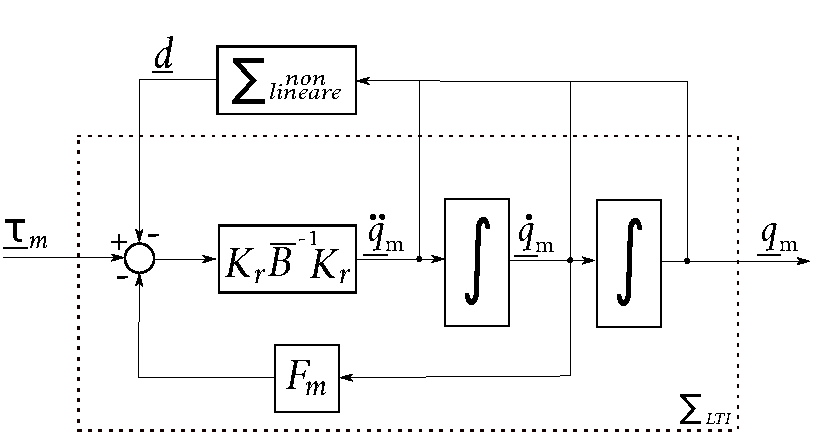
\includegraphics[scale=0.6]{controlloDecentralizzato.pdf}
	\caption{Sistema manipolatore e azionamenti.}
\end{center}
in pratica il sistema costituito dal manipolatore e dagli azionamenti si presenta come costituito da due sottosistemi:
\begin{enumerate}
	\item Il sistema con ingresso $\underline{\tau}_{\,m}$ e uscita $\underline{q}_{\,m}$ è \textbf{lineare e disaccoppiato} nel senso che ogni componente di $\underline{\tau}_{\,m}$ influenza solamente la corrispondente componente di $\underline{q}_{\,m}$.
	\item Il sistema con ingresso $\underline{q}_{\,m}$, $\underline{\dot{q}}_{\,m}$, $\underline{\ddot{q}}_{\,m}$ e uscita $\underline{d}$ è \textbf{non lineare e accoppiato} in quanto porta in conto tutti quei contributi che evidenziano come posizione e moto di ogni giunto si influenzino mutuamente con effetti non lineari di interazione.
\end{enumerate}

\paragraph{}
Il progetto della legge di controllo porta ad una struttura decentralizzata del controllore, in quanto ogni giunto è visto in maniera indipendente dagli altri. Modelliamo la parte non lineare $\underline{d}$ come ingressi non manipolabili di disturbo per gli azionamenti dei singoli giunti. 

Il controllore di giunto deve garantire elevate prestazioni in termini di forte reiezione ai disturbi e di capacità di inseguimento di traiettorie di riferimento. \emph{La struttura di controllo è basata sull'errore tra uscita desiderata e uscita effettiva, e la coppia sintetizzata dall'algoritmo di controllo per l'attuatore $i$ dipende solo dalla valutazione dell'errore associato all'uscita $i$}.

\paragraph{}
Pertanto il processo da controllare è l'azionamento del giunto $i$ controllato in tensione, corrispondente ad un sistema a un ingresso e una uscita della parte lineare e disaccoppiata, chiaramente l'interazione con gli altri giunti è descritta dalla componente $i$ del vettore $\underline{d}$, lo schema risulta il seguente

\begin{center}
	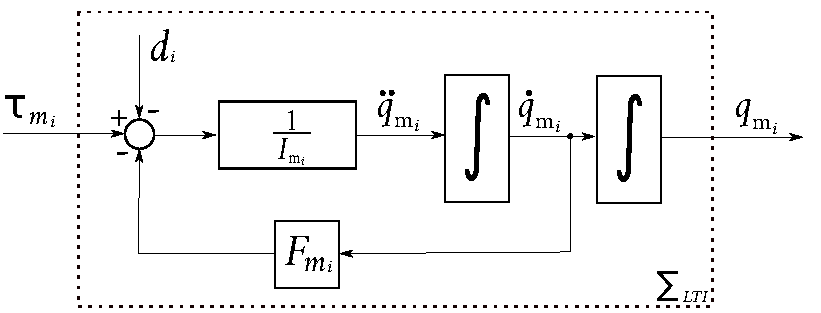
\includegraphics[scale=0.6]{decentralizzatoDisaccoppiato.pdf}
	\caption{Sistema LTI disaccoppiato.}
\end{center}

con $F_{m_i}$ la $i$-esima componente della matrice diagonale $K_r^{-T} F_v K_r^{-1}$ e $1/I_{m_i}$ la $i$-esima componente della matrice diagonale $K_r \overline{B}^{-1} K_r$.

\paragraph{}
Si utilizza in controllo decentralizzato quando:
\begin{itemize}
	\item Non sono richieste prestazioni troppo elevate in termini di precisioni del controllo $\dot{q}$, $\ddot{q}$.
	\item $K_r$ è una matrice "\emph{grossa}", ovvero $K_r^{-T} = K_r^{-1}$, quindi i rapporti di trasmissione $N_i$ elevati e filtrano la dinamica dal resto del manipolatore.
\end{itemize}


\subsection{Controllo di posizione}
Nel capitolo sugli azionamenti (capitolo 7) abbiamo esaminato la progettazione del sistema di attuazione, ovvero le modalità di cui è possibile avvalersi per controllare la velocità di rotazione dell'albero di un servomotore (elettrico). Adesso esaminiamo il problema del controllo del moto di un braccio di un generico manipolatore.

Ricorriamo a una struttura che sia in grado di determinare, in modo automatico, l'andamento temporale della grandezza scelta per controllare il motore, in modo che essa faccia eseguire al giunto interessato il movimento richiesto per consentire all'organo terminale di eseguire un determinato compito. 

\paragraph{}
La soluzione del problema è quella di considerare il moto di un giunto indipendente dal moto degli altri giunti e modellare i fenomeni di interazione come disturbi. Sia $\vartheta_r$ la traiettoria di riferimento data in ingresso come traiettoria desiderata, sia $\vartheta_m$ posizione angolare dell'asse del motore misurata da un trasduttore con costante $K_{TP}$ e sia il servomotore elettrico a corrente continua. 

Con riferimento all'azionamento pilotato in tensione di figura ($7.3$), trascurando l'induttanza $L_a$ e l'attrito $F_m$, otteniamo
\begin{equation}
	\frac{\Omega(s)}{V_a(s)} = \frac{\frac{1}{k_v}}{1+ \frac{R_a I_m}{k_v k_t} s} = \frac{k_m}{1+ T_m s}
\end{equation}

e lo schema generale di controllo dell'azionamento con retroazione di posizione è il seguente,

\begin{center}
	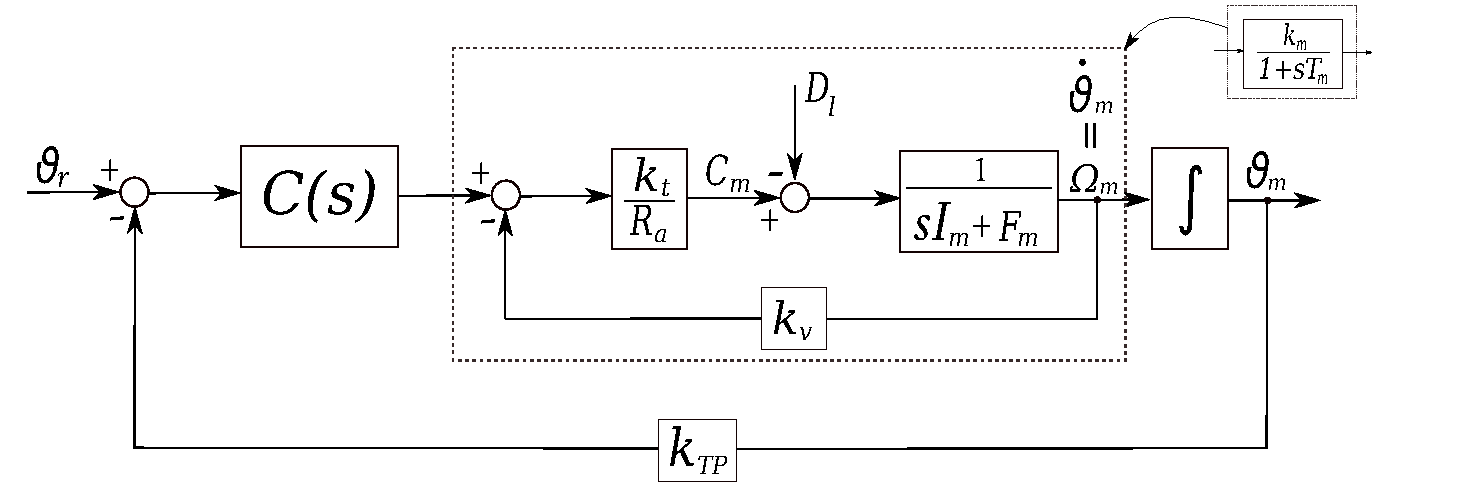
\includegraphics[scale=0.5]{controlloAzionamentoElettrico.pdf}
	\caption{Schema generale di controllo di una azionamento elettrico}
\end{center}
in pratica, il controllore posto in \emph{retroazione dinamica sull'uscita} deve garantire la reiezione dei disturbi e l'inseguimento al riferimento con minimo errore possibile. Pertanto, focalizziamoci sulla ricerca del controllore.

\paragraph{}
I requisiti del controllore che stiamo cercando sono dettati dalla riduzione degli effetti del disturbo sull'uscita. Pertanto necessitiamo di
\begin{itemize}
	\item Un alto guadagno a monte del punto di applicazione del disturbo.
	\item Un'azione integrale che annulla l'effetto della componente gravitazionale. sull'uscita.
\end{itemize}
questi requisiti suggeriscono di impiegare sulla linea di azione diretta un controllore \emph{proporzionale-integrale} (PI). Per migliorare le \emph{prestazioni dinamiche}, ovvero, ridurre ulteriormente gli effetti del disturbo, conviene realizzare il controllore come una cascata di azioni elementari e la chiusura di anelli locali di retroazione che contengano al loro interno il punto di applicazione del disturbo.

La soluzione più completa si ottiene con la chiusura di anelli interni di posizione, velocità e accelerazione,
\begin{center}
	\includegraphics[scale=0.3]{schemaGeneraleControlloPosizione.pdf}
	\caption{Struttura generale di controllo indipendente al giunto.}
\end{center}
esaminando lo schema otteniamo:
\begin{itemize}
	\item $C_{P}(s)$, $C_{V}(s)$, $C_{A}(s)$ sono i controllori di \emph{posizione}, \emph{velocità} e \emph{accelerazione}.
	\item $k_{TP}$, $k_{TV}$, $k_{TA}$ sono le rispettive costanti di trasduzione di posizione, velocità e accelerazione.
	\item Il disturbo $D$ è scalato di una costante $R_a/k_t$ (vedi riduzione a blocchi nelle appendici)
\end{itemize} 
infine notiamo l'ingresso di riferimento $\vartheta_r$ è legata all'uscita desiderata $\vartheta_{md}$ attraverso la relazione $\vartheta_r = k_{TP} \vartheta_{md}$, illustrata di seguito
\begin{center}
	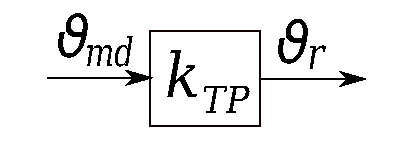
\includegraphics[scale=0.4]{trasduttoreIniziale.pdf}
	\caption{Legame tra \emph{riferimento} e \emph{uscita desiderata}.}
\end{center}
si considerano \emph{tre} casi di studio che si distinguono tra loro per il numero di cicli di retroazione attivati.

\subsubsection{\underline{Retroazione di Posizione:}}
In questo caso l'azione di controllo è caratterizzata da 
\begin{equation*}
	C_P(s) = K_P \frac{1+sT_P}{s} \qquad C_V(s) = 1 \qquad C_A(s) = 1 
\end{equation*}
con $k_{TV} = k_{TA} = 0$ la struttura generale mostrata in ($9.6$) diventa
\begin{center}
	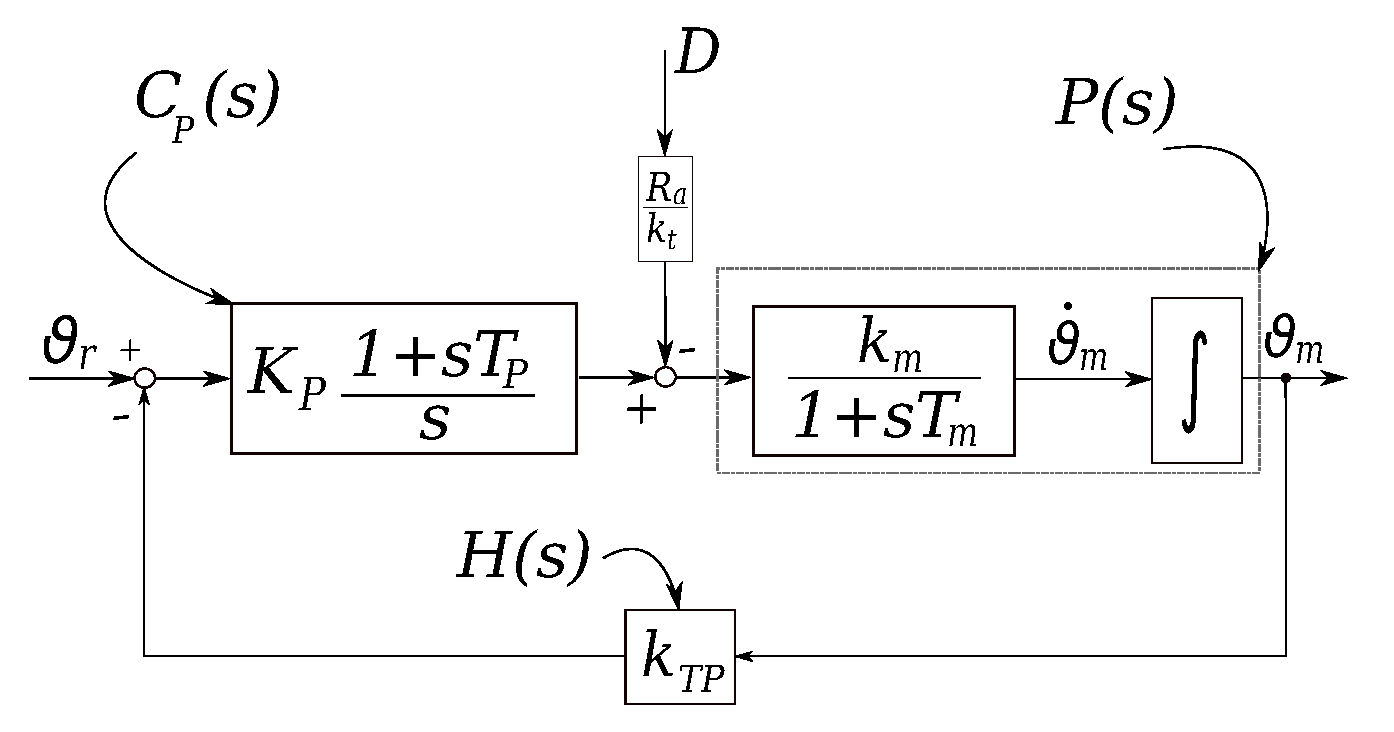
\includegraphics[scale=0.35]{schemaPos.pdf}
	\caption{Schema di controllo con retroazione di posizione.}
\end{center}
con $P(s)$ l'impianto da controllare, $H(s)$ la retroazione e la coppia $(K_P, T_P)$ rappresenta i \emph{parametri del controllore}.

La \emph{f.d.t.} ingresso-uscita in anello chiuso vale
\begin{equation}
	\frac{\vartheta_m(s)}{\vartheta_r(s)} = \frac{\frac{1}{k_{TP}}}{1+\frac{s^2(1+sT_m)}{k_mK_pk_{TP}(1+sT_P)}}
\end{equation}

La \emph{f.d.t.} disturbo-uscita vale
\begin{equation}
	\frac{\vartheta_m(s)}{D(s)} = - \frac{\frac{sR_a}{k_tK_Pk_{TP}(1+sT_P)}}{1+\frac{s^2(1+sT_m)}{k_mK_Pk_{TP}(1+sT_P)}}
\end{equation}
notiamo che l'azione integrale manda a $0$ il disturbo, infatti usando il \emph{TVF} otteniamo
\begin{equation*}
	\lim_{t \rightarrow \infty} \vartheta(t) = \lim_{s \rightarrow 0} s \vartheta(s) = \lim_{s \rightarrow 0} - \frac{R_a}{k_t} \frac{1}{k_{TP}K_P} \Bigl( s \frac{s}{(\cdots)} \frac{D}{s} \Bigr) = 0
\end{equation*} 
e se non è presente l'azione integrale si ottiene 
\begin{equation*}
	\lim_{t \rightarrow \infty} \vartheta(t) = \lim_{s \rightarrow 0} s \vartheta(s) = \lim_{s \rightarrow 0}  - \frac{R_a}{k_t} \frac{D}{\underbrace{(k_{TP}K_P)}_{X_R}} \neq 0
\end{equation*}
notiamo che il termine $X_R = k_{TP}K_P$ è il \emph{fattore di reiezione del disturbo} determinato dal guadagno $K_P$, ovvero il fattore di riduzione del disturbo. 

\paragraph{}
Definiamo la dinamica dell'azionamento attraverso l'uso del luogo delle radici (le regole per determinarlo sono nell'Appendice $B$) esaminando la funzione ad anello $L(s)$ in dipendenza della scelta del parametro $T_P$. Otteniamo
\begin{itemize}
	\item[a)] \textbf{\underline{Se $T_P < T_m$:}} Scegliamo $T_P = \frac{T_m}{2}$, lo zero è $\frac{-1}{T_P}=\frac{-2}{T_m}$, i poli sono $\lbrace 0, 0, \frac{-1}{T_m} \rbrace$. L'eccesso poli zeri è $n-m=3-1=2$, le direzioni degli asintoti sono: $\frac{\pi}{2}$, $\frac{3 \pi}{2}$ e il punto di incontro degli asintoti è $\frac{1}{2 T_m}$. Pertanto risulta che vi saranno sempre coppie di poli con pare reale maggiore di zero e quindi il sistema è instabile.
	\item[b)] \textbf{\underline{Se $T_P > T_m$:}} Scegliamo $T_P = 2T_m$, lo zero è $\frac{-1}{T_P}=\frac{-2}{T_m}$, i poli sono $\lbrace 0, 0, \frac{-1}{T_m} \rbrace$. L'eccesso poli zeri è $n-m=3-1=2$, il punto di incontro degli asintoti è $\frac{-1}{4 T_m}$. Pertanto risulta che il sistema è stabile perché i tre poli stanno tutti nel semipiano con la parte reale negativa. Ma vi è un problema, lo smorzamento dei poli dominanti (quelli più vicini all'asse immaginario, ovvero i più lenti) è insoddisfacente, in pratica, vi è una sovraelongazione.
	\item[c)] \textbf{\underline{Se $T_P \gg T_m$:}} Scegliamo $T_P = 10 T_m$, pertanto il punto di incontro degli asintoti è $\frac{-9}{20 T_m}$. Con questa scelta riesco a trovare tre poli con smorzamento unitario, pertanto il polo dominante è $ \simeq \frac{-1}{T_P}$
\end{itemize}

\begin{center}
	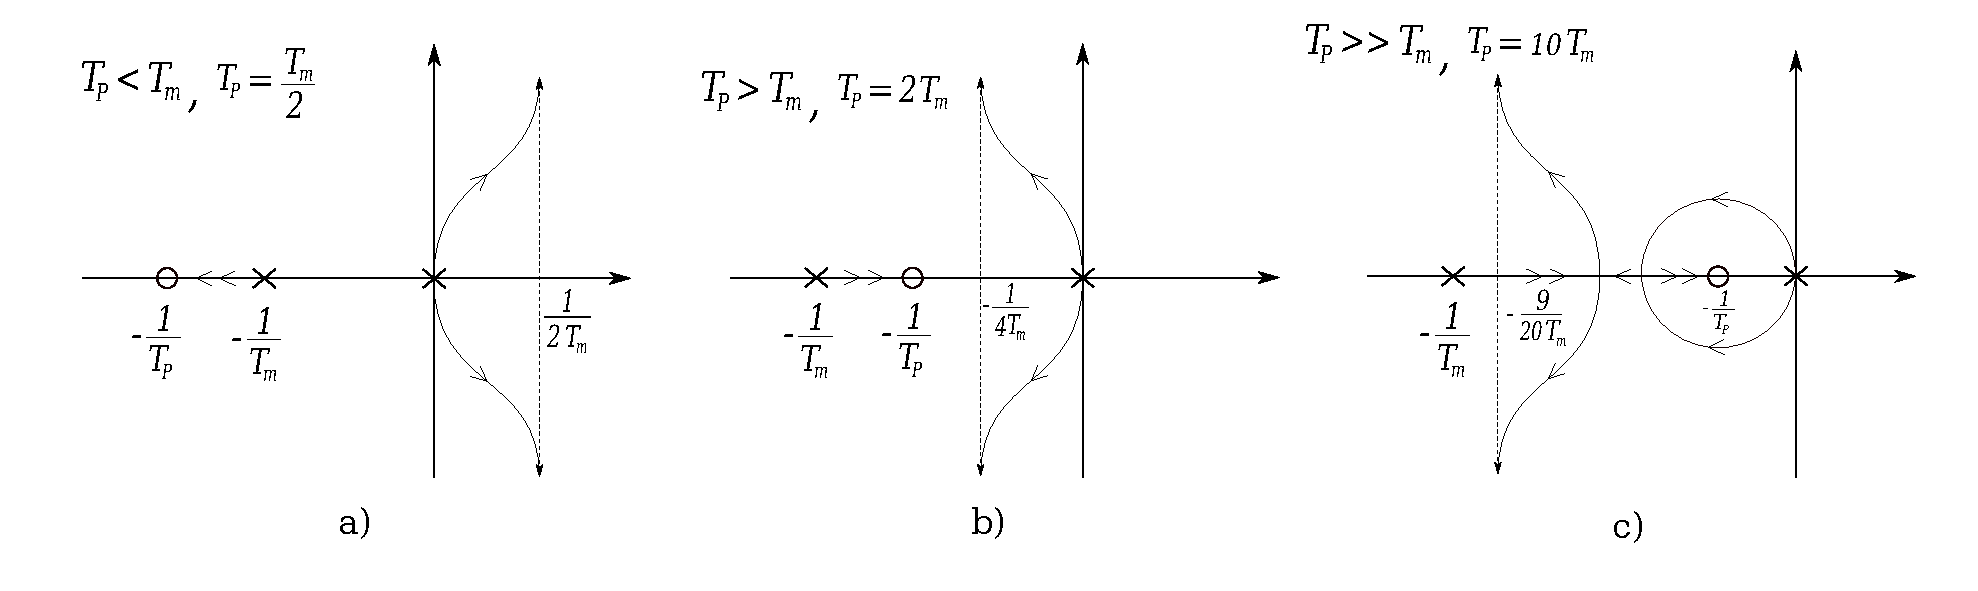
\includegraphics[scale=0.45]{rlocusPos.pdf}
	\caption{Luogo delle radici per lo schema di controllo con retroazione di posizione.}
\end{center}

\paragraph{}
La \emph{f.d.t.} ingresso-uscita nella ($9.7$) può essere espressa nella forma
\begin{equation}
	W(s) = \frac{\frac{1}{k_{TP}} (1+sT_P)}{\Bigl( 1 + \frac{2\zeta s}{\omega_n} + \frac{s^2}{\omega_n^2} \Bigr)(1+s\tau)} 
\end{equation}
dove $\omega_n$ e $\zeta$ sono rispettivamente la pulsazione naturale e il coefficiente di smorzamento della coppia di poli complessi coniugati e $-1/\tau$ è il polo reale.

Definiamo tempo di reiezione del disturbo per disturbi costanti $T_R$, come
\begin{equation}
	T_R = \max \Bigl\lbrace T_P, \frac{1}{\zeta \omega_n} \Bigr\rbrace
\end{equation}
con $\tau \approx T_P$.

\subsubsection{\underline{Retroazione di Posizione e Velocità:}}
In questo caso l'azione di controllo è caratterizzata da 
\begin{equation*}
	C_P(s) = K_P  \qquad C_V(s) = K_V \frac{1+sT_V}{s} \qquad C_A(s) = 1 
\end{equation*}
con $k_{TA} = 0$ la struttura generale mostrata in ($9.6$) diventa
\begin{center}
	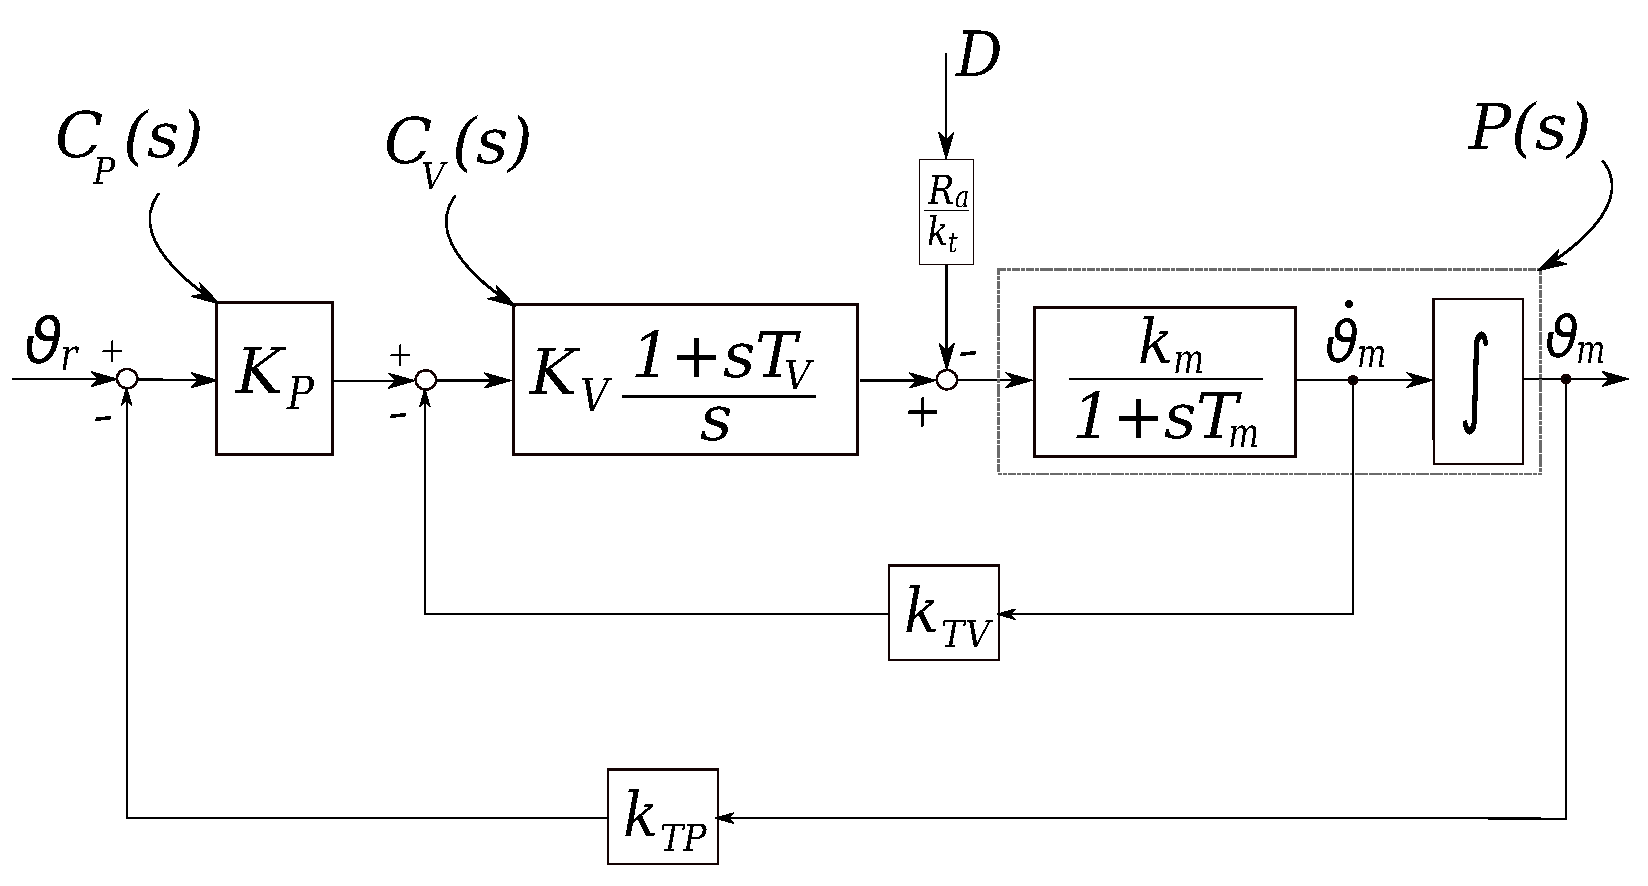
\includegraphics[scale=0.35]{schemaPosVel.pdf}
	\caption{Schema di controllo con retroazione di posizione e velocità.}
\end{center}
con $(K_P, K_V, T_V)$ \emph{parametri di progetto}. 

La \emph{f.d.t.} del ramo di azione diretta vale
\begin{equation}
	G(s) = \frac{k_m K_P K_V (1+sT_V)}{s^2(1+sT_m)}
\end{equation}
e quella del ramo di retroazione vale
\begin{equation}
	H(s) = k_{TP} \Bigl( 1+s\frac{k_{TV}}{K_Pk_{TP}} \Bigr)
\end{equation}
ponendo $T_V = T_m$ cancelliamo il polo reale del motore $s = -\frac{1}{T_m}$ con il polo reale $s = -\frac{1}{T_V}$.

\paragraph{}
La \emph{f.d.t.} ingresso-uscita in anello chiuso vale
\begin{equation}
	\frac{\vartheta_m(s)}{\vartheta_r(s)} = \frac{\frac{1}{k_{TP}}}{1+ \frac{sk_{TV}}{K_Pk_{TP}}+\frac{s^2}{k_mK_Pk_{TP}K_V}}
\end{equation}
equivalentemente 
\begin{equation}
	W(s) = \frac{\frac{1}{k_{TP}}}{1+2\frac{\zeta s}{\omega_n} + \frac{s^2}{\omega_n^2}}
\end{equation}
supponendo $\zeta$ e $\omega_n$ assegnati, si ottengono le seguenti relazioni di progetto
\begin{equation}
	\begin{cases}
		K_Vk_{TV} = \frac{2 \zeta \omega_n}{k_m} \\
		K_Pk_{TP}K_V = \frac{\omega_n^2}{k_m} 
	\end{cases}
\end{equation}

\paragraph{}
La \emph{f.d.t.} disturbo-uscita vale
\begin{equation}
	\frac{\vartheta_m(s)}{D(s)} = - \frac{\frac{s R_a}{k_tK_Pk_{TP}K_V(1+sT_m)}}{1+\frac{sk_{TV}}{K_Pk_{TP}}+\frac{s^2}{k_mK_Pk_{TP}K_V}}
\end{equation}
pertanto, il \emph{fattore di reiezione del disturbo} sull'uscita è pari a $X_R = K_P k_{TP}K_V$.

\paragraph{}
Esaminiamo il luogo delle radici, considerando
\begin{equation}
	L(s) = \frac{K_P K_V k_m k_{TP}}{s^2} \Bigr( 1 + \frac{k_{TV}s}{K_P k_{TP}} \Bigl)
\end{equation}
l'incremento del guadagno di posizione $K_P$ consente di posizionare i poli del sistema in anello chiuso in regioni del piano complesso caratterizzate da elevati valori assoluti della parte reale, definendone poi, l'allocazione puntuale con una opportuna scelta di $K_V$. Gli zeri sono $\lbrace \frac{-1}{T_V}, \frac{-k_{TP}K_P}{k_{TV}} \rbrace$, i poli invece $\lbrace 0,0,\frac{-1}{T_m} \rbrace$.
\begin{center}
	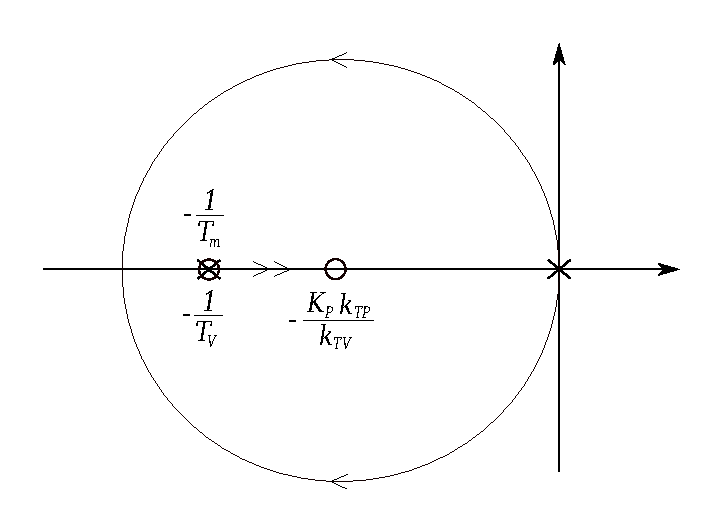
\includegraphics[scale=0.4]{rlocusPosVel.pdf}
	\caption{Luogo delle radici per lo schema con retroazione di posizione e velocità.}
\end{center} 
esaminando il \emph{tempo di recupero} $T_R$, si ha
\begin{equation}
	T_R = \max \lbrace T_m, \frac{1}{\zeta \omega_n} \rbrace 
\end{equation}
se piazzo lo zero di $H(s)$, tramite un $K_P$ più grande, a sinistra della coppia cancellata, il sistema migliora in termini di prontezza e notiamo un miglioramento rispetto alla sola retroazione di posizione, ma $T_R$ resta uguale.

\subsubsection{\underline{Retroazione di Posizione, Velocità e Accelerazione:}}
In questo caso l'azione di controllo è caratterizzata da 
\begin{equation*}
	C_P(s) = K_P  \qquad C_V(s) = K_V  \qquad C_A(s) = K_A\frac{1+sT_A}{s} 
\end{equation*}
con tutti i trasduttori $\neq 0$, la struttura generale mostrata in ($9.6$) diventa
\begin{center}
	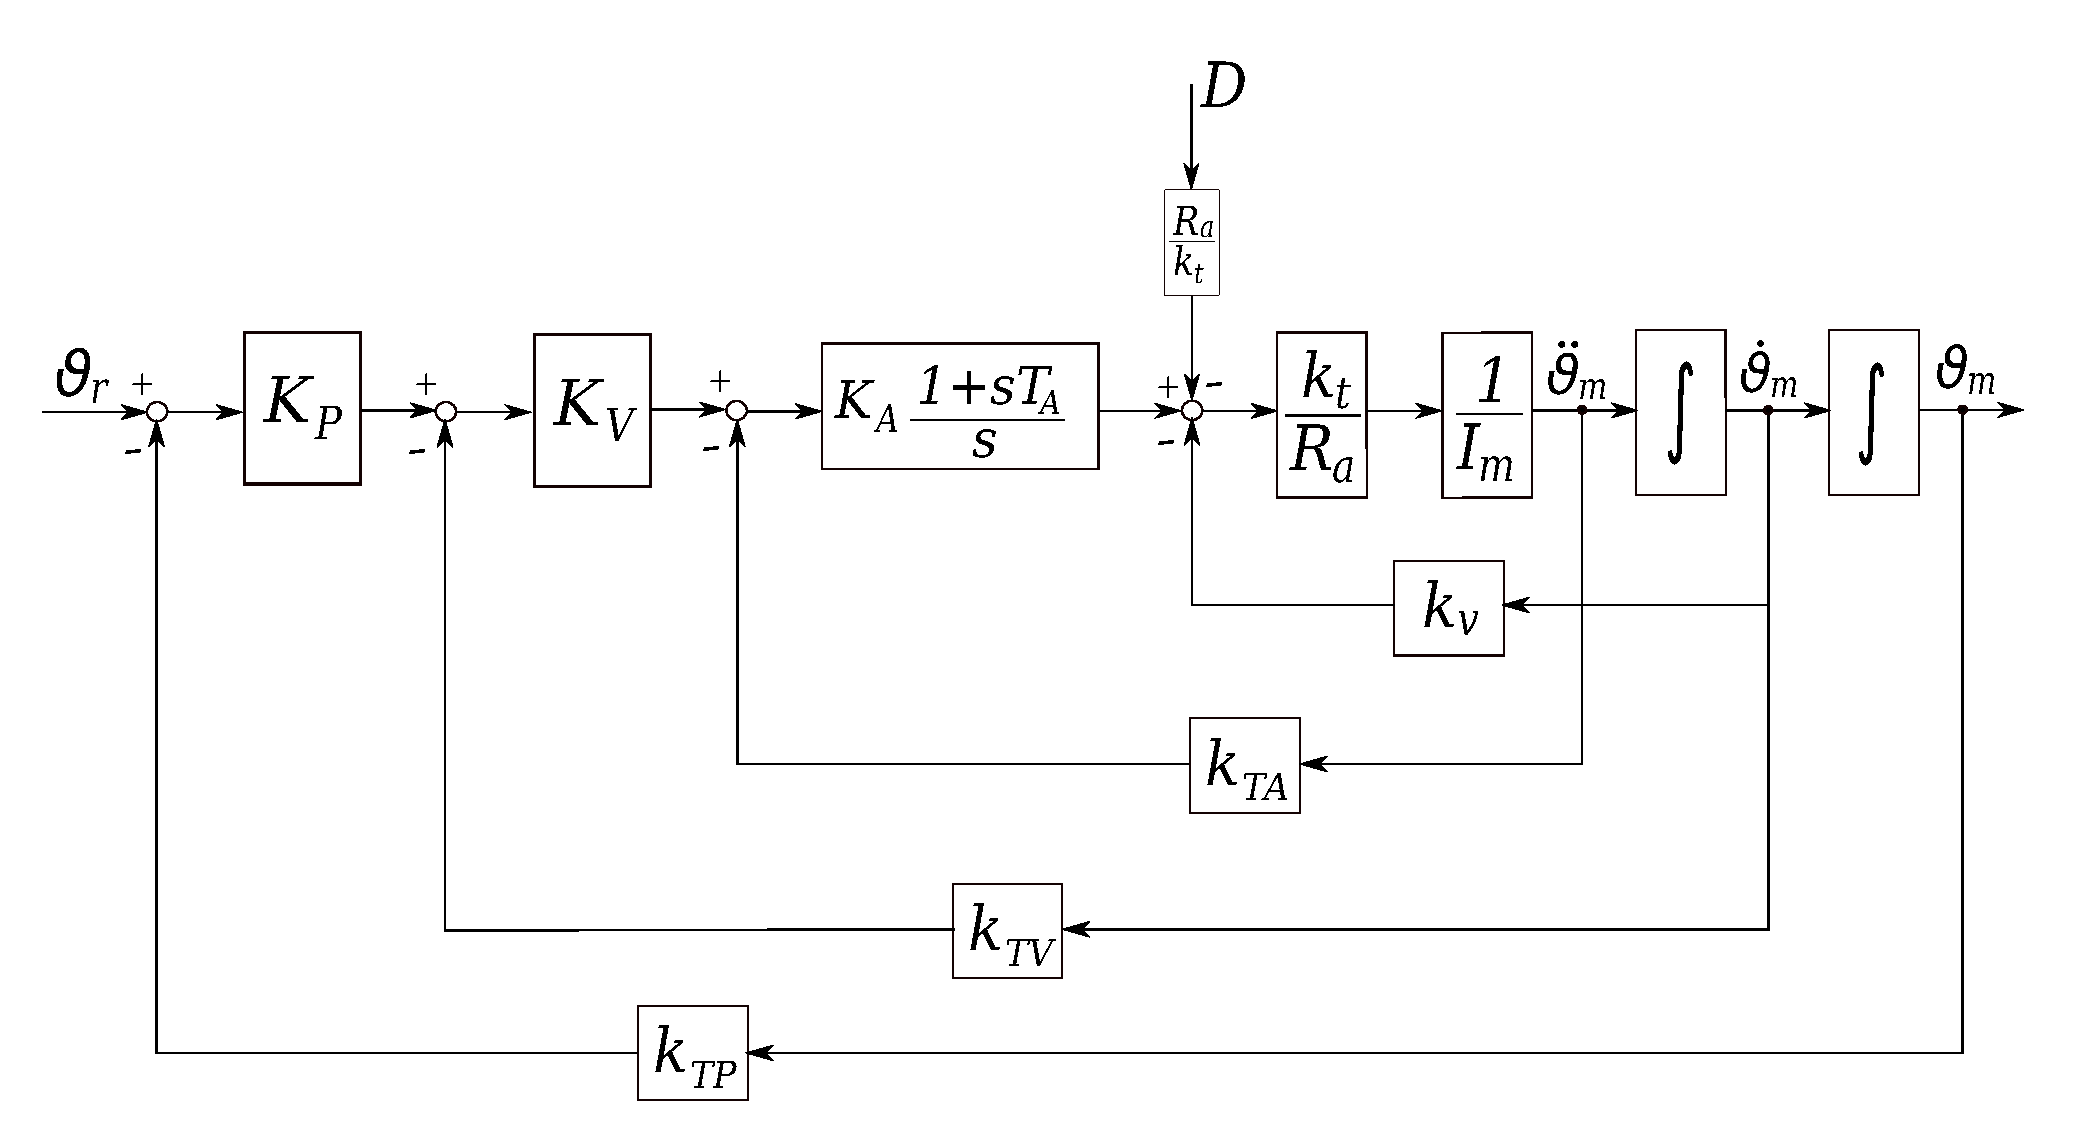
\includegraphics[scale=0.35]{schemaPosVelAcc.pdf}
	\caption{Schema di controllo con retroazione di posizione, velocità e accelerazione.}
\end{center}
con $(K_P, K_V, K_A, T_A)$ \emph{parametri di progetto}. 

La \emph{f.d.t.} del ramo di azione diretta vale 
\begin{equation*}
	G(s) = \Biggl( \frac{K_P K_V K_A (1+sT_A)}{s^2} \Biggr) \Biggl( \frac{k_m}{(1+k_mK_Ak_{TA})\Bigl( 1+\frac{sT_m(1+k_mK_Ak_{TA}\frac{T_A}{T_m})}{(1+k_mK_Ak_{TA})} \Bigr)} \Biggr)
\end{equation*}

La \emph{f.d.t.} del ramo di retroazione vale
\begin{equation}
	H(s) = k_{TP}\Bigl( 1+ \frac{sk_{TV}}{K_Pk_{TP}} \Bigr)
\end{equation}

\paragraph{}
Abbiamo due modi per cancellare il polo del motore 
\begin{itemize}
	\item In maniera diretta, $T_A = T_m$, in questo caso ottengo $T_R = T_m = T_A$ e mi riconduco al caso di retroazione di posizione e velocità.
	\item In maniera indiretta, ponendo
	\begin{equation}
		k_mK_Ak_{TA}T_A \gg T_m \qquad k_mK_Ak_{TA} \gg 1
	\end{equation}
	così facendo la costante $T_A$ rimane libera e posso sceglierla $< T_m$.
\end{itemize}

\paragraph{}
Facendo la seconda scelta, consideriamo 
\begin{equation}
	L(s) = \Bigl( \frac{k_{TV}K_VK_Ak_m}{1+k_{TA}K_Ak_m} \Bigr) \Bigl( \frac{s+\frac{k_{TP} K_P}{k_{TV}}}{s^2} \Bigr)
\end{equation}
e il luogo delle radici risulta,
\begin{center}
	\includegraphics[scale=0.4]{rlocusPosVelAcc.pdf}
	\caption{Luogo delle radici per il controllo con retroazione di posizione, velocità e accelerazione.}
\end{center}

\paragraph{}
La \emph{f.d.t.} ingresso-uscita in anello chiuso è
\begin{equation}
	\frac{\vartheta_m(s)}{\vartheta_r(s)} = \frac{\frac{1}{k_{TP}}}{1+\frac{sk_{TV}}{K_Pk_{TP}}+\frac{s^2(1+k_mKAk_{TA})}{k_mK_Pk_{TP}K_VK_A}}
\end{equation}

La \emph{f.d.t.} disturbo-uscita è
\begin{equation}
	\frac{\vartheta_m(s)}{D(s)} = -\frac{\frac{s R_a}{k_tK_Pk_{TP}K_VK_A(1+sT_A)}}{1+\frac{sk_{TV}}{K_Pk_{TP}}+\frac{s^2(1+k_mK_Ak_{TA})}{k_mK_Pk_{TP}K_VK_A}}
\end{equation}

Pertanto, il \emph{fattore di riduzione} è il seguente
\begin{equation}
	X_R = K_Pk_{TP}K_VK_A
\end{equation}
e il \emph{tempo di recupero} è caratterizzato da
\begin{equation}
	T_R = \max \lbrace T_A, \frac{1}{\zeta \omega_n} \rbrace
\end{equation}
con $T_A$ controllabile.

\paragraph{}
Con riferimento alla funzione tipica del secondo ordine $W(s)$ riportata in ($9.14$), otteniamo con analogia alle relazioni in ($9.15$), le seguenti equazioni,
\begin{equation}
	\begin{cases}
		\frac{2K_Pk_{TP}}{k_{TV}} = \frac{\omega_n}{\zeta} \\
		k_mK_Ak_{TA} = \frac{k_mX_R}{\omega_n^2} - 1\\
		K_Pk_{TP}K_VK_A = X_R
	\end{cases}
\end{equation}
notiamo che la retroazione di accelerazione consente di ottenere, un qualsiasi comportamento dinamico desiderato e inoltre rispetto ai casi precedenti, consente di prefissare il fattore di riduzione degli effetti indotti dal disturbo.

\newpage

\subsection{Misura di grandezze retroazionate} 
Le tre soluzioni di controllo fino adesso illustrate trascurano un problema fondamentale che si presenta nella pratica, ovvero, la misura delle grandezze da retroazionare. Infatti, non vi è alcun problema nel misurare posizione e velocità, mentre una misura diretta dell'accelerazione non è disponibile e risulta onerosa da ottenere. 

Nel retroazionare l'accelerazione nella terza soluzione illustrata nella Figura 9.12, possiamo ricorrere a una misura indiretta, ovvero, ricostruiamo la grandezza \emph{accelerazione} con un \textit{\textbf{filtro del primo ordine}}.
\begin{center}
	\includegraphics[scale=0.4]{filtroDerivata.pdf}
	\caption{Filtro ricostruttore della \emph{derivata}.}
\end{center}

Il filtro ricostruisce l'operazione di \emph{derivazione} ed è caratterizzato da una banda passante a 3 dB $\omega_{3f} = k_f$. Scegliendo tale banda sufficientemente ampia, gli effetti dei ritardi indotti nella misura possono ritenersi trascurabili e quindi è lecito utilizzare come grandezza da retroazionare l'uscita in accelerazione del filtro.

Posso ricorrere alla \emph{tecnica del filtraggio} anche se ho solo la posizione come grandezza disponibile, infatti, ricorrendo ad un filtro del \emph{secondo} ordine, posso ricostruire sia la velocità che l'accelerazione. Chiaramente ho più errori e difficoltà di implementazione numerica del controllore.

\subsection{Compensazione in avanti decentralizzata}
Quando si considerano azionamenti a cui sono imposte traiettorie desiderate in posizione caratterizzate da elevati valori di velocità e accelerazioni, le capacità di \textbf{inseguimento} presentate dallo schema ($9.6$) sono degradate. 

L'adozione di un'azione di \emph{compensazione in avanti decentralizzata} consente di ridurre l'errore di inseguimento a meno dell'effetto dei disturbi. I nuovi ingressi risultano,
\begin{align}
	\vartheta_r(s) = \Bigl( k_{TP} + \frac{s^2(1+sT_m)}{k_mK_p(1+sT_P)}  \Bigr) \vartheta_{md}(s) \\
	\vartheta_r(s) = \Bigl( k_{TP} + s\frac{k_{TV}}{K_P} + \frac{s^2}{k_mK_PK_V} \Bigr) \vartheta_{md}(s) \\
	\vartheta_r(s) = \Bigl( k_{TP} + s\frac{k_{TV}}{K_P} \frac{s^2(1+k_mK_Ak_{TA})}{k_mK_PK_VK_A}\Bigr) \vartheta_{md}(s)
\end{align}
in tal modo si ottiene l'inseguimento della posizione desiderata $\vartheta_{md}(s)$. I tre schemi risultanti si ottengono attraverso semplici manipolazione in catena diretta da $\vartheta_r(s)$ negli schemi 9.8, 9.10 e 9.12. Otteniamo
\begin{center}
	\includegraphics[scale=0.35]{compensazioneAvantiPos.pdf}
	\caption{Retroazione di posizione con compensazione in avanti decentralizzata.}
	
	\includegraphics[scale=0.35]{compensazioneAvantiPosVel.pdf}
	\caption{Retroazione di posizione e velocità con compensazione in avanti decentralizzata.}
	
	\includegraphics[scale=0.35]{compensazioneAvantiPosVelAcc.pdf}
	\caption{Retroazione di posizione, velocità e accelerazione con compensazione in avanti decentralizzata.}
\end{center}

\paragraph{}
Notiamo che al crescere del numero di anelli interni, si riduce la conoscenza del sistema di attuazione necessaria per la realizzazione dell'azione in avanti. Infatti,
\begin{itemize}
	\item Per lo schema in figura 9.15 è richiesta la conoscenza di $T_m$ e $k_m$.
	\item Per lo schema in figura 9.16 è richiesta la conoscenza di $k_m$.
	\item Per lo schema in figura 9.17 è richiesta la conoscenza di $k_m$ ma con peso ridotto.
\end{itemize}

Questa soluzione, presenta delle \emph{non linearità} intenzionali la cui funzione è quella di limitare, nei transitori, grandezze fisiche di particolare interesse. Al crescere del numero di anelli di retroazione aumenta il numero di grandezze su cui è possibile effettuare operazioni di limitazione (velocità, accelerazione e tensione del motore). 

\paragraph{}
Possiamo individuare delle \emph{strutture di controllo equivalenti} che utilizzano la sola retroazione di posizione e regolatori con azioni standard. Queste strutture hanno le stesse caratteristiche di reiezione dei disturbi e inseguimento di riferimenti, però l'eliminazione degli anelli di retroazione interni toglie la possibilità di inserire limitazioni sulla velocità e sulla accelerazione. 

Le \emph{azioni di controllo} in questi nuovi schemi hanno le seguenti \emph{equivalenze},
\begin{itemize}
	\item Retroazione di posizione $\Longleftrightarrow$ PI.
	\item Retroazione di posizione e velocità $\Longleftrightarrow$ PID.
	\item Retroazione di posizione, velocità e accelerazione $\Longleftrightarrow$ PIDD$^2$.
\end{itemize}
pertanto gli schemi equivalenti alle figure 9.15, 9.16, 9.17 sono rispettivamente
\begin{center}
	\includegraphics[scale=0.35]{PI.pdf}
	\caption{Retroazione di posizione di tipo PI, equivalente allo schema 9.15}
	
	\includegraphics[scale=0.35]{PID.pdf}
	\caption{Retroazione di posizione di tipo PID, equivalente allo schema 9.16}
	
	\includegraphics[scale=0.35]{PIDD.pdf}
	\caption{Retroazione di posizione di tipo PIDD$^2$, equivalente allo schema 9.17}
\end{center}
notando che queste strutture sono tutte caratterizzate dalla presenza dell'azione in avanti $(\frac{T_m}{k_m})\dot{\vartheta}_{md} + (\frac{1}{k_m}) \dot{\vartheta}_{md}$.

\subsection{Riepilogo}
Facciamo un prospetto riassuntivo del \textbf{controllo decentralizzato} visto fino adesso,
\begin{center}
	\includegraphics[scale=0.56]{riassuntoDecentralizzato.pdf}
\end{center}

\section{Controllo Centralizzato}
Fino adesso, abbiamo considerato gli effetti di interazione e accoppiamento tra i diversi giunti come \emph{cause di disturbo} agenti su ogni singolo azionamento. Quando però abbiamo un manipolatore con attuatori ad accoppiamento diretto o attuatori ad alta velocità di movimento, i termini non lineari di accoppiamento influenzano in maniera massiva le prestazioni del sistema, per cui considerare l'effetto delle componenti di $\underline{d}$ come disturbi può generare errori notevoli nell'inseguimento di traiettorie desiderate.

Pertanto, è necessario agire sulla \emph{eliminazione delle cause di disturbo} piuttosto che sulla riduzione degli \emph{effetti del disturbo}, generando delle coppie (o forze) che vadano a compensare gli effetti dell'interazione espressi dal vettore $\underline{d}$ in ($9.5$). Useremo quindi, \emph{schemi di controllo centralizzato} basati sulla conoscenza, parziale o completa, del modello dinamico del manipolatore.

\paragraph{}
\textbf{\textit{Come mostrato dal modello matematico $(9.1)$, il manipolatore non è un insieme di n sistemi disaccoppiati ma è un sistema multivariabile, con n ingressi (le coppie ai giunti) ed n uscite (le posizioni dei giunti) tra di loro interagenti con legami di tipo non lineare.}}

\paragraph{}
L'obiettivo è quello di inseguire una traiettoria $\underline{q}_{\,d}$, $\dot{\underline{q}}_{\,d}$, $\ddot{\underline{q}}_{\,d}$ con sistema di errore globalmente, asintoticamente stabile. Affrontiamo il problema della determinazione della legge $\underline{\tau}$ che assicura il soddisfacimento di prestazioni al sistema manipolatore-attuatori considerato.

\subsection{Controllo PD con compensazione di gravità}
Sia assegnata una postura costante di equilibrio con un vettore di posizione desiderate ai giunti $\underline{q}_{\,d}$. Mediante la chiusura di anelli di posizione su ogni giunto, si vuole individuare la struttura del controllore che assicuri la stabilità asintotica globale della posizione di equilibrio. Lo stato è il vettore,
\begin{equation}
	\begin{bmatrix}
		\underline{e} \\
		\underline{\dot{q}}
	\end{bmatrix}
\end{equation}
dove $\underline{e} = \underline{q}_{\,d} - \underline{q}$ rappresenta l'errore di posizione.

\paragraph{}
Utilizziamo il \emph{metodo diretto di Lyapunov} per determinare il vettore di controllo che garantisce la stabilizzazione del punto di equilibrio. Si scelga come candidata di Lyapunov, la forma quadratica definita positiva
\begin{equation}
	V(\dot{\underline{q}}, \underline{e}) = \frac{1}{2} \underline{\dot{q}}^T B(\underline{q})\underline{\dot{q}} + \frac{1}{2} \underline{e}^T K_P \underline{e} > 0 \qquad \forall\underline{\dot{q}}, \underline{e} \neq 0
\end{equation}
con $K_P \in \mathbb{R}^{n \times n}$ simmetrica e definita positiva. Una interpretazione energetica evidenzia un primo termine che rappresenta l'energia cinetica della struttura e un secondo termine che rappresenta l'energia elastica di un sistema di molle con rigidità $K_P$ realizzato dagli $n$ anelli di retroazione di posizione.

Derivando la candidata e ricordando che $\underline{q}_{\,d}$ è costante, otteniamo,
\begin{equation}
	\dot{V} = \underline{\dot{q}}^T B(\underline{q}) \ddot{\underline{q}} + \frac{1}{2}\underline{\dot{q}}^T \dot{B}(\underline{q}) \underline{\dot{q}} + \underline{e}^T K_P \underline{\dot{e}} = \underline{\dot{q}}^T \Bigl( -K_P \underline{e} + B \underline{\ddot{q}} + \frac{1}{2} \dot{B}\underline{\dot{q}} \Bigr)
\end{equation}
adesso consideriamo
\begin{equation}
	\ddot{q} = B^{-1}(\underline{q}) \Bigl( \underline{\tau} - C(\underline{q}, \underline{\dot{q}})\underline{\dot{q}} - F_v \underline{\dot{q}} - \underline{g}(\underline{q}) \Bigr)
\end{equation}
e sostituendo alla ($9.32$),
\begin{equation}
	\dot{V} = \underline{\dot{q}}^T \Bigl( -K_P \underline{e} + \underline{\tau} - C \underline{\dot{q}} - F_v \underline{\dot{q}} - \underline{g}(\underline{q}) + \frac{1}{2} \dot{B} \underline{\dot{q}} \Bigr)
\end{equation}
e adesso ricordando che la matrice $\dot{B} - 2C$ è antisimmetrica, la proprietà che ci viene in aiuto per questa dimostrazione di stabilità è
\begin{equation}
	\underline{\dot{q}}^T \Bigl( \frac{1}{2} \dot{B} - C \Bigr) \underline{\dot{q}} = 0
\end{equation}
adesso troviamo un $\underline{\tau}$ tale che $\dot{V} < 0$,
\begin{itemize}
	\item Mettiamo un termine $K_P \underline{e}$ per neutralizzare $- K_P \underline{e}$.
	\item Mettiamo un termine $\underline{g}(\underline{q})$ per compensare la gravità $-\underline{g}(\underline{q})$.
	\item Mettiamo un termine che renda ancora più negativo $\dot{V}$, ovvero, una retroazione tachimetrica $- K_D \underline{\dot{q}}$ con $K_D$ definita positiva.
\end{itemize}
otteniamo la seguente legge di controllo,
\begin{equation}
	\underline{\tau} = K_P \underline{e} - K_D \underline{\dot{q}} + \underline{g}(\underline{q})
\end{equation}
e riscrivendo la ($9.34$) otteniamo
\begin{equation}
	\dot{V} = - \underline{\dot{q}}^T (F_v + K_D)\underline{\dot{q}}
\end{equation}
che evidenzia quanto il termine derivativo $K_D$ renda il sistema più pronto.

\paragraph{}
La dinamica del sistema controllato con la legge ($9.36$) è espressa da
\begin{equation}
	B(\underline{q})\underline{\ddot{q}} + C(\underline{q}, \underline{\dot{q}})\underline{\dot{q}} + \underline{g}(\underline{q}) = \underline{g}(\underline{q}) + K_P \underline{e} - K_D \underline{\dot{q}}
\end{equation}
e all'equilibrio ($\underline{\dot{q}} = 0$, $\underline{\ddot{q}} = 0$) si ottiene
\begin{equation}
	K_P \underline{e} = \underline{0} \Rightarrow \underline{e} = 0
\end{equation}
che è la postura di equilibrio cercata.

\begin{center}
	\includegraphics[scale=0.4]{centralizzatoPDgravita.pdf}
	\caption{Schema di controllo PD ai giunti con compensazione di gravità.}
\end{center}

\subsubsection{Discorso qualitativo:}
Quanto visto fino adesso \underline{dimostra} che qualunque postura di equilibrio del manipolatore risulta globalmente asintoticamente stabile se il controllo esplica un'azione lineare di tipo PD e un'azione non lineare di compensazione degli effetti gravitazionali. Pertanto la stabilità è assicurata con una scelta qualsiasi delle matrici $K_D$ e $K_P$ purchè siano definite positive.

\subsection{Controllo a Dinamica Inversa}
Consideriamo il problema dell'inseguimento di una traiettoria specificata nello spazio dei giunti. Il modello dinamico di un manipolatore a $n$ giunti è espresso dalla seguente relazione
\begin{equation}
	B(\underline{q})\underline{\ddot{q}} + n(\underline{q}, \underline{\dot{q}}) = \underline{\tau}
\end{equation}
con $n(\underline{q}, \underline{\dot{q}}) = C(\underline{q}, \underline{\dot{q}})\underline{\dot{q}} + F_v \underline{\dot{q}} + \underline{g}(\underline{q})$.

\paragraph{}
L'idea è quella di individuare un vettore di controllo $\underline{\tau}$, funzione dello stato del sistema, che sia in grado di realizzare relazioni ingresso-uscita che presentino caratteristiche lineari. L'obiettivo è quello di effettuare una \emph{linearizzazione esatta} mediante una retroazione \emph{non lineare} dello stato del sistema. Quindi \underline{non} una linearizzazione locale. 

Assumiamo la seguente legge di controllo,
\begin{equation}
	\underline{\tau} = \hat{B}(\underline{q})\underline{y} + \hat{n}(\underline{q}, \underline{\dot{q}})
\end{equation}
denominata \textbf{controllo a dinamica inversa} perchè si basa sul calcolo della dinamica inversa del manipolatore. A questo punto, poniamo l'uguaglianza
\begin{equation}
	B(\underline{q})\underline{\ddot{q}} + n(\underline{q}, \underline{\dot{q}}) = \hat{B}(\underline{q})\underline{y} + \hat{n}(\underline{q}, \underline{\dot{q}})
\end{equation}
e se la linearizzazione è esatta, otteniamo $\underline{n} = 0$, $B^{-1}\hat{B} = I$, ovvero un sistema costituito da un banco di integratori doppi.

Pertanto, il sistema è descritto dall'equazione $\underline{\ddot{q}} = \underline{y}$ con $\underline{y}$ nuovo vettore di ingresso la cui struttura deve ancora essere determinata.

\paragraph{}
Il sistema sotto la legge di controllo appena descritta, risulta \emph{lineare} e \emph{disaccoppiato} nei riguardi del nuovo ingresso $\underline{y}$. Ovvero, la componente $y_i$ influenza con un legame di doppia integrazione, solo la variabile di giunto $q_i$, indipendentemente dal moto degli altri giunti. Scegliamo,
\begin{equation}
	\underline{y} = \underline{\ddot{q}}_{\,d} + K_D \underline{\dot{e}} + K_P \underline{e}
\end{equation}
con $K_D$ e $K_P$ \emph{definite positive} e \emph{diagonali}, otteniamo il seguente sistema di equazioni
\begin{equation}
	\begin{cases}
		\underline{\ddot{q}} = \underline{y} \\
		\underline{y} = \underline{\ddot{q}}_{\,d} + K_D \underline{\dot{e}} + K_P \underline{e}
	\end{cases}
	\Rightarrow \quad
	\underbrace{\underline{\ddot{q}}_{\,d} - \underline{\ddot{q}}}_{\underline{\ddot{e}}} + K_D \underline{\dot{e}} + K_P \underline{e} = \underline{0}
\end{equation}
Quindi, il sistema risulta descritto dall'equazione,
\begin{equation}
	\underline{\ddot{e}} = -K_P \underline{e} - K_D \underline{\dot{e}} = 
	\begin{bmatrix}
		- K_P & - K_D
	\end{bmatrix}
	\underbrace{
	\begin{bmatrix}
		\underline{e} \\
		\underline{\dot{e}}
	\end{bmatrix}
	}_{\underline{\xi}}
\end{equation}
definendo $\underline{\xi}$ lo \emph{stato del sistema}, il sistema che si ottiene è $LTI$, scriviamo l'evoluzione dello stato,
\begin{equation}
	\underline{\dot{\xi}} = \frac{d}{dt} 
	\begin{bmatrix}
		\underline{e} \\
		\underline{\dot{e}}
	\end{bmatrix}
	= 
	\underbrace{
	\begin{bmatrix}
		0 & I \\
		-K_P & - K_D \\
	\end{bmatrix}
	}_{A}
	\begin{bmatrix}
		\underline{e} \\
		\underline{\dot{e}}
	\end{bmatrix}	
\end{equation} 
tutti gli autovalori di $A$ hanno parte reale negativa, quindi abbiamo la stabilità asintotica globale.

\paragraph{}
Troviamo gli autovalori con il polinomio caratteristico per un singolo asse $i$,
\begin{equation}
	\ddot{e}_i + K_{D_i} \dot{e}_i +K_{P_i} e_i = 0 \qquad \forall i = 1, \cdots, n
\end{equation}
con 
\begin{equation}
	\xi_i = 
	\begin{bmatrix}
		e_i \\
		\dot{e}_i \\
	\end{bmatrix}
	\quad
	A = 
	\begin{bmatrix}
		0 & 1 \\
		-K_{P_i} & -K_{D_i}
	\end{bmatrix}
\end{equation}
pertanto,
\begin{equation}
	\det(sI-A) = s^2 + K_{D_i}s + K_{P_i} = 0 \Rightarrow 
	\begin{cases}
		\zeta = \frac{K_{D_i}}{2 \sqrt{K_{P_i}}} \\
		\omega_n^2 = K_{P_i}
	\end{cases}
\end{equation}
con queste caratteristiche si garantisce inseguimento perfetto, e inoltre notiamo come l'errore converga a zero con una velocità di risposta dipendente dalle matrici $K_D$ e $K_P$. 

\subsubsection{Discorso qualitativo}
Lo schema del controllo a dinamica inversa risulta,
\begin{center}
	\includegraphics[scale=0.4]{centralizzatoDinamicaInversa.pdf}
	\caption{Schema di controllo a dinamica inversa ai giunti.}
\end{center}
dove possiamo notare la presenza di due anelli di retroazione,
\begin{itemize}
	\item l'anello interno basato sul modello dinamico del manipolatore e ha la funzione di rendere disponibile un legame ingresso-uscita lineare e disaccoppiato,
	\item l'anello esterno opera sull'errore e ha il compito di stabilizzare il sistema complessivo.
\end{itemize}
Questa tecnica di compensazione non lineare a disaccoppiamento è interessante perchè va ad effettuare una sostituzione della dinamica del manipolatore non lineare con $n$ sottosistemi lineari tra di loro non interagenti. 

\subsection{Computer Torque Control}
Questa tecnica è usata dalle più importanti aziende produttrici di Robot, si tratta di una compensazione in avanti a coppia precalcolata che fa uso sia del controllo centralizzato che di quello decentralizzato. 

Con riferimento allo schema più generale in Figura 9.20, la grandezza di uscita del PIDD$^2$ è costituita dalla funzione 
\begin{equation}
	a_2 \ddot{e} + a_1 \dot{e} a_0 e + a_{-1} \int_0^t e(\sigma) d\sigma
\end{equation}
che rappresenta l'evoluzione nel tempo dell'errore. Con riferimento allo schema seguente,
\begin{center}
	\includegraphics[scale=0.4]{dinamicaCTC.pdf}
\end{center}
costruiamo uno schema con
\begin{itemize}
	\item L'azione di \emph{feedback} rappresentata dalla ($9.50$)
	\item L'azione di \emph{feedforward} decentralizzata rappresentata da
		\begin{equation}
			\frac{T_m}{k_m} \ddot{\vartheta_{md}} + \frac{1}{k_m} \dot{\vartheta_{md}}
		\end{equation}
	\item Il disturbo, espresso come
		\begin{equation}
			-\frac{R_a}{k_t}\cdot d
		\end{equation}
\end{itemize}

\paragraph{}
L'obiettivo è quello di eliminare l'errore e il disturbo, ottenendo $\dot{\vartheta}_{md} = \dot{\vartheta_m}$ e $\ddot{\vartheta}_{md} = \ddot{\vartheta}_d$, pertanto desideriamo la seguente uguaglianza,
\begin{equation}
	a_2 \ddot{e} + a_1 \dot{e} a_0 e + a_{-1} \int_0^t e(\sigma) d\sigma + \frac{T_m}{k_m} \ddot{\vartheta_{md}} + \frac{1}{k_m} \dot{\vartheta_{md}} -\frac{R_a}{k_t}\cdot d = \frac{T_m}{k_m} \ddot{\vartheta_{m}} + \frac{1}{k_m} \dot{\vartheta_{m}}
\end{equation}
modificando i coefficienti ($a'_1 \triangleq a_1 + \frac{T_m}{k_m}$), scriviamo
\begin{equation}
	a'_2 \ddot{e} + a'_1 \dot{e} a'_0 e + a'_{-1} \int_0^t e(\sigma) d\sigma = \frac{R_a}{k_t} \cdot d
\end{equation}
tale equazione mostra che ogni traiettoria fisicamente eseguibile è asintoticamente seguita (a regime) se il termine di disturbo $d(t) = 0$.

\paragraph{}
La presenza del termine $d(t)$ comporta la nascita di un errore di inseguimento caratterizzato dalla \emph{f.d.t.}
\begin{equation}
	\frac{E(s)}{D(s)} = \frac{s \frac{R_a}{k_t}}{a'_2 s^3 + a'_1 s^2 + a'_0 s + a'_{-1}}
\end{equation}
notiamo che lo zero nell'origine va a reiettare a regime $D(s)$.

\paragraph{}
Si può aggiungere ai precedenti segnali di azioni in avanti un termine che sia in grado di compensare non gli effetti del disturbo ma il disturbo stesso. Siano $\underline{q}_{\,d}(t)$ la traiettoria desiderata per i giunti e $\underline{q}_{\,md}(t)$ la corrispondente traiettoria per gli attuatori. Utilizziamo l'azione in avanti
\begin{equation}
	R_a K_t^{-1} \underline{d}_{\,d}
\end{equation}
con
\begin{equation}
	\underline{d}_{\,d} = K_r^{-1} \Delta B(\underline{q}_{\,d}) K_r^{-1} \underline{\ddot{q}}_{\,md} + K_r^{-1} C(\underline{q}_{\,d}, \underline{\dot{q}}_{\,d}) K_r^{-1} \underline{\dot{q}}_{\,md} + K_r^{-1}\underline{g}(\underline{q}_{\,d})
\end{equation}
dove $R_a$ e $K_t$ denotano le matrici diagonali delle resistenze di armatura e delle costanti di coppia degli attuatori. L'azione in avanti della ($9.56$) tende a compensare il disturbo $\underline{d}$ espresso dalla ($9.5$). Le schema di questo controllo è
\begin{center}
	\includegraphics[scale=0.4]{ComputerTorqueControl.pdf}
	\caption{Schema di controllo CTC.}
\end{center}
e rappresenta in forma compatta il sistema di controllo di un manipolatore che realizza algoritmi di controllo del tipo  a coppia precalcolata. Notiamo

\begin{itemize}
	\item Il sistema di controllo in retroazione è rappresentativo degli $n$ sistemi di controllo dei singoli giunti considerati indipendenti, esso è \textbf{decentralizzato} in quanto il controllore $i$ di giunto elabora riferimenti e misure relativi a grandezze caratteristiche del solo giunto $i$.
	\item Le interazioni esistenti tra i diversi giunti, espresse dal disturbo $\underline{d}$, vengono compensate da \textbf{un'azione centralizzata} la cui funzione è quella di generare un'azione in avanti che dipende dai riferimenti di tutti i giunti e dal modello dinamico del manipolatore.
	\item L'azione centralizzata compensa i termini non lineari di accoppiamento dovuti alle coppie inerziali, di Coriolis, centrifughe e gravitazionali che dipendono dalla struttura e si modificano durante il movimento del manipolatore.
\end{itemize}
\chapter{Pianificazione di traiettorie}
L'obiettivo della pianificazione di traiettorie è quello di generare ingressi di riferimento per il sistema di controllo del moto che assicuri l'esecuzione da parte del manipolatore delle traiettorie pianificate. Definiamo:
\begin{itemize}
	\item \textbf{Percorso:} è il luogo dei punti dello spazio operativo che il manipolatore deve descrivere nell'esecuzione del movimento assegnato. Pertanto la descrizione è di tipo \emph{geometrica}.
	\item \textbf{Traiettoria:} è un \emph{percorso} su cui sia specificata una \underline{legge oraria} di moto.
\end{itemize}
In linea di principio, un \emph{algoritmo} di pianificazione della traiettoria avrà il seguente schema
\begin{center}
	\includegraphics[scale=0.3]{algoritmoTraiettorie.pdf}
\end{center}
dove l'uscita è rappresentata dalle traiettorie dell'organo terminale espresse come sequenze di posa, velocità e accelerazione. Questo algoritmo generico, può operare nello spazio dei giunti che in quello operativo.

\section{Spazio dei giunti}
La specificazione di un particolare movimento viene usualmente effettuata assegnando, nello \emph{spazio operativo}, alcuni parametri della traiettoria, come
\begin{itemize}
	\item posa iniziale e finale dell'organo terminale,
	\item eventuali pose intermedie dell'organo terminale,
	\item tempi di percorrenza di alcuni percorsi geometrici.
\end{itemize}
Se si vuole pianificare una traiettoria nello \emph{spazio dei giunti}, a partire dalle posiziono e dagli orientamenti assegnati all'organo terminale bisogna preventivamente ricavare i valori delle variabili di giunti corrispondenti alle pose fissate dall'utente.

\paragraph{}
L'algoritmo di pianificazione genera una funzione $\underline{q}(t)$ che interpola i valori assegnati per le variabili di giunto nel rispetto dei vincoli imposti. In generale all'algoritmo si richiedono le seguenti caratteristiche:
\begin{itemize}
	\item Necessariamente:
	\begin{itemize}
		\item $q(t)$ funzione continua
		\item $\dot{q}(t)$ funzione continua
	\end{itemize}
	\item Se riusciamo, vogliamo anche:
	\begin{itemize}
		\item $\ddot{q}(t)$ funzione continua
		\item la funzione $Jerk$, definita come $j(t) = \frac{d}{dt} \ddot{q}(t)$ limitata
	\end{itemize}
\end{itemize}
ovvero, gli obiettivi della pianificazione delle traiettorie.


\subsection{Moto punto-punto}
Il manipolatore deve muoversi da una configurazione iniziale di variabili di giunto, ad una configurazione finale in un tempo fissato. Pertanto, si richiede di portare la variabile angolare $q$ da un valore iniziale $q_i$ ad un valore finale $q_f$ in un intervallo di tempo $t_f$. Chiaramente, si possono individuare infinite funzioni che compiono questo tragitto
\begin{center}
	\includegraphics[scale=0.3]{infiniteConfigurazioni.pdf}
\end{center}
ma l'algoritmo dovrà generare una traiettoria che vada a ottimizzare, in relazione ad un qualche \emph{indice di qualità}, lo spostamento di $q$.

\paragraph{}
Andiamo a modellare il sistema con
\begin{equation}
	I\ddot{q} = \tau
\end{equation}
e impostiamo un problema di ottimo vincolato, ovvero cerchiamo $\dot{q}(t)$ tale che
\begin{itemize}
	\item minimizzi l'indice di qualità $\int_0^{t_f} \tau^2(\sigma) d \sigma$
	\item soddisfi il vincolo $\int_0^{t_f} \dot{q}(\sigma) d \sigma  = q_f - q_i$
\end{itemize}
il risultato è che $q(t)$ sarà un \emph{polinomio cubico}, ovvero con \emph{velocità parabolica}. 
\subsubsection{\underline{Profilo Parabolico:}}
Risulta quindi,
\begin{align}
	q(t) = a_3 t^3 + a_2 t^2 + a_1 t + a_0 \\
	\dot{q}(t) = 3 a_3 t^2 + 2 a_2 t + a_1 \\
	\ddot{q}(t) = 6 a_3 t + 2 a_2
\end{align}

\begin{center}
	\includegraphics[scale=0.3]{velocitaParabolica.pdf}
	\caption{Andamento temporale con legge oraria della velocità parabolica.}
\end{center}
Abbiamo quindi, guardando la ($10.2$), quattro coefficienti $a_0$, $a_1$, $a_2$ e $a_3$ su cui possiamo lavorare e andare a imporre $q_i$, $q_f$, $\dot{q}_i$ e $\dot{q}_f$. Non possiamo imporre nulla sulle accelerazioni. In quel caso, dobbiamo usare un polinomio di quinto grado per $q(t)$.

\subsubsection{\underline{Profilo Trapezoidale:}}
Un approccio alternativo con leggi orarie di tipo polinomiale \emph{misto} che viene adottato spesso nella pratica industriale è quello del \emph{profilo trapezoidale di velocità}, che impone un'accelerazione costante nella fase di partenza, una velocità di crociera e una decelerazione costante nella fase di arrivo.

La traiettoria che ne risulta è costituita da un tratto lineare \emph{raccordato} con due tratti parabolici nell'intorno della posizione finale e iniziale.

\begin{center}
	\includegraphics[scale=0.3]{velocitaTrapezoidale.pdf}
	\caption{Andamento temporale con legge oraria trapezoidale della velocità.}
\end{center}
nei grafici abbiamo supposto che la velocità iniziale e finale siano nulle. Vediamo adesso i \emph{metodi di pianificazione} del profilo di velocità trapezoidale,
\begin{itemize}
	\item \textbf{Assegnati $q_i$, $q_f$, $t_f$, $\ddot{q}_c$ :} vogliamo rispettare il vincolo sull'area del trapezio, otteniamo pertanto
		\begin{equation*}
			\int_0^{t_f} \dot{q}(\sigma) d\sigma = q_f - q_i \quad \Rightarrow \quad 
			\begin{cases}
				q_f - q_i = (t_f - t_c) \dot{q}_c \\
				\dot{q}_c = \ddot{q}_c t_c 
			\end{cases}
			\quad \Rightarrow \quad q_f - q_i = \ddot{q}_c t_f t_c - \ddot{q}_c t_c^2
		\end{equation*}
		e quindi 
		\begin{equation*}
			t_c^2 - t_f t_c +  \frac{q_f - q_i}{\ddot{q}_c} = 0 \quad \Rightarrow \quad t_c = \frac{t_f}{2} \pm \frac{\sqrt{t_f^2 - 4 \frac{q_f - q_i}{\ddot{q}_c}}}{2}
		\end{equation*}
		guardando il dominio naturale della radice,
		\begin{equation*}
			t_f^2 \geqslant 4 \frac{q_f - q_i}{\ddot{q}_c} \quad \Rightarrow \quad \vert \ddot{q}_c \vert \geqslant 4 \frac{\vert q_f - q_i \vert}{t_f^2}
		\end{equation*}
		e notiamo che se scegliamo l'accelerazione con l'uguaglianza
		\begin{equation}
			\vert \ddot{q}_c \vert = 4 \frac{\vert q_f - q_i \vert}{t_f^2}
		\end{equation}
		otteniamo un \emph{profilo triangolare di velocità}, perchè la traiettoria \underline{non} presenta il tratto a velocità costante, ma solo i tratti di accelerazione e decelerazione. Pertanto, avendo $q_i$, $q_f$, $t_f$, calcolando $\ddot{q}_c$ e $t_c$ si generano le funzioni polinomiali seguenti
		\begin{equation}
			q(t) = 
			\begin{cases}
				q_i + \frac{1}{2} \ddot{q}_c t^2 \qquad \qquad \;\;\; 0 \leqslant t \leqslant t_c \\
				q_i + \ddot{q}_c t_c (t- \frac{t_c}{2}) \qquad t_c < t \leqslant t_f - t_c \\
				q_i - \frac{1}{2} \ddot{q}_c (t_f - t)^2 \qquad t_f - t_c < t \leqslant t_f
			\end{cases}
		\end{equation}			
	
	\item \textbf{Assegnati $q_i$, $q_f$, $t_f$, $\dot{q}_c$ :} Anche in questo caso partiamo dal vincolo, ma stavolta non esplicitiamo $\dot{q}_c$ perchè non abbiamo l'accelerazione,
		\begin{equation*}
			(t_f - t_c) \dot{q}_c = q_f - q_i \quad \Rightarrow \quad t_f - t_c = \frac{q_f - q_i}{\dot{q}_c} \quad \Rightarrow \quad t_c = t_f - \frac{q_f - q_i}{\dot{q}_c}
		\end{equation*}
		a questo punto guardando la Figura 10.2 notiamo due cose:
		\begin{enumerate}
			\item $t_c > 0$, ovvero
				\begin{equation*}
					t_f > \frac{q_f - q_i}{\dot{q}_c} \quad \Rightarrow \quad \vert \dot{q}_c \vert > \frac{\vert q_f - q_i \vert}{t_f}
				\end{equation*}
			\item $t_c \leqslant \frac{t_f}{2}$, ovvero
				\begin{equation*}
					t_f - \frac{q_f - q_i}{\dot{q}_c} \leqslant \frac{t_f}{2} \quad \Rightarrow \quad \vert \dot{q}_c \vert \leqslant 2 \frac{\vert q_f - q_i \vert}{t_f}
				\end{equation*}
		\end{enumerate}
		quindi otteniamo,
		\begin{equation}
			\frac{\vert q_f - q_i \vert}{t_f} < \vert \dot{q}_c \vert \leqslant 2 \frac{\vert q_f - q_i \vert}{t_f}
		\end{equation}
		e quindi possiamo ricavare $t_c$ e $\ddot{q}_c$ riconducendoci alle equazioni ($10.6$).
	\item \textbf{Assegnati $q_i$, $q_f$, $\dot{q}_c$, $\ddot{q}_c$ :} In questo caso, abbiamo
		\begin{equation}
			\dot{q}_c = \ddot{q}_c t_c \quad \Rightarrow \quad t_c = \frac{\dot{q}_c}{\ddot{q}_c} 
		\end{equation}
		ma l'accelerazione è discontinua e pertanto il Jerk è infinito. Spesso è preferibile ammorbidire la fase di accelerazione utilizzando, ad esempio le \emph{S-curve}. Il grafico del trapezio risulta più morbido nei punti di raccordo.
\end{itemize}

\subsection{Sequenza di punti}
Affrontiamo adesso, il problema di generazione della traiettoria quando siano specificati $N$ punti di cammino (\emph{waypoint}), che devono essere raggiunti dal manipolatore in determinati istanti. In linea di principio si può pensare di usare un solo polinomio di grado $N-1$ che passi per tutti i punti. Ma abbiamo svariati problemi,
\begin{itemize}
	\item Non possiamo assegnare velocità iniziale e finale.
	\item Più il grado aumenta e più aumenta il suo carattere oscillatorio.
	\item Sistema di calcolo oneroso, ecc...
\end{itemize}
pertanto, invece di considerare un singolo polinomio di grado elevato, andiamo a considerare un \emph{insieme di polinomi interpolatori} di grado più basso uniti tra di loro nei punti di cammino. Abbiamo visto precedentemente che il grado più basso è il terzo perchè ci garantisce la continuità della velocità nei punti di cammino.

\paragraph{} 
Facendo riferimento ad una singola variabile di giunto, si deve individuare una funzione $q(t)$, costituita da una sequenza di polinomi cubici
\begin{equation}
	\Pi_k(t) \quad \dot{\Pi}_k(t) \quad \ddot{\Pi}_k(t) \qquad  k = 1, \cdots, N-1
\end{equation}
che assuma valori $q_k$ per $t = t_k$ ($k = 1, \cdots, N$) con $q_1 = q_i$, $t_1 = 0$, $q_N = q_f$, $t_N = t_f$. 
\begin{center}
	\includegraphics[scale=0.3]{traiettoria.pdf}
	\caption{Waypoint}
\end{center}
con il generico polinomio $\Pi_k(t)$ che raccorda $q_k$ con $q_{k+1}$. I valori di $\dot{q}(t)$ in corrispondenza dei punti di cammino possono essere scelti arbitrariamente. Ma possiamo effettuare una scelta più saggia, indicando con $v_k$ la pendenza della spezzata nell'intervallo di tempo $[t_{k-1}, t_k]$
\begin{equation}
	v_k = \frac{(q_k - q_{k-1})}{(t_k - t_{k-1})}
\end{equation}
utilizziamo le seguenti regole:
\begin{equation}
	\begin{cases}
		\dot{q}_1 = 0 \\
		\dot{q}_N = 0 \\
		\dot{q}_k = 
		\begin{cases}
			0 \qquad \qquad \qquad \quad \text{con $v_k$, $v_{k+1}$ discordi} \\
			\frac{1}{2} (v_k + v_{k+1}) \qquad \text{con $v_k$, $v_{k+1}$ concordi}
		\end{cases}
	\end{cases}
\end{equation}

\paragraph{}
Adesso andiamo a porre le condizioni iniziali,
\begin{equation}
	\begin{cases}
		\Pi_1(t_1) = q_1 \\
		\dot{\Pi}_1(t_1) = 0 \\
		\ddot{\Pi}_1(t_1) = 0 
	\end{cases}
	\qquad
	\begin{cases}
		\Pi_{N-1}(t_N) = q_N \\
		\dot{\Pi}_{N-1}(t_N) = 0 \\
		\ddot{\Pi}_{N-1}(t_N) = 0 
	\end{cases}
\end{equation}
e per ogni $k \in (1,N)$ \emph{punti intermedi} scriviamo quattro equazioni:
\begin{itemize}
	\item Una equazione di passaggio per $q_k$.
	\item Tre equazioni che pongono le \emph{condizioni di continuità} della posizione, velocità e accelerazione.
\end{itemize}
e risulta
\begin{equation}
	\begin{cases}
		\Pi_{k-1}(t_k) = q_k \\
		\Pi_{k-1}(t_k) = \Pi_{k}(t_k) \\
		\dot{\Pi}_{k-1}(t_k) = \dot{\Pi}_{k}(t_k) \\
		\ddot{\Pi}_{k-1}(t_k) = \ddot{\Pi}_{k}(t_k)
	\end{cases}
\end{equation}
e si ottengono pertanto $4N-2$ equazioni nei $4(N-1)$ coefficienti incogniti. Per rendere il sistema \emph{quadrato} perchè vogliamo usare solo polinomi di terzo grado, andiamo ad aggiungere due \emph{punti virtuali} su cui è possibile imporre vincoli di continuità su posizione, velocità e accelerazione. Notiamo come \emph{non} importa la collocazione di questi due punti virtuali in quanto andiamo a imporre vincoli solo sulla continuità. 

Consideriamo quindi $N+2$ istanti di tempo $t_k$, dove $t_2$ e $t_{N+1}$ individuano convenzionalmente i punti virtuali introdotti. Otteniamo,

\begin{equation}
t_2: 
\begin{cases}
	\Pi_1(t_2) = \Pi_2(t_2) \\
	\dot{\Pi}_1(t_2) = \dot{\Pi}_2(t_2) \\
	\ddot{\Pi}_1(t_2) = \ddot{\Pi}_2(t_2) 
\end{cases}
\;
t_{N+1}:
\begin{cases}
	\Pi_N(t_{N+1}) = \Pi_{N+1}(t_{N+1}) \\
	\dot{\Pi}_N(t_{N+1}) = \dot{\Pi}_{N+1}(t_{N+1}) \\
	\ddot{\Pi}_N(t_{N+1}) = \ddot{\Pi}_{N+1}(t_{N+1})
\end{cases}
\end{equation}
ne risulta un sistema di $4(N+1)$ equazioni per la determinazione dei $4(N+1)$ coefficienti degli $N+1$ polinomi cubici.

\section{Spazio operativo}
Con la pianificazione di traiettorie nello spazio dei giunti si genera, sulla base di primitive di movimento, una sequenza temporale dei valori che le variabili giunto $q(t)$ devono assumere in modo che il manipolatore si porti dalla configurazione iniziale a quella finale, passando eventualmente attraverso una serie di configurazioni intermedie.

Quando si desidera che il moto si sviluppi su un percorso di caratteristiche geometriche definite nello \emph{spazio operativo}, è necessario pianificare le traiettorie direttamente nello stesso spazio. 

\subsection{Posizione}
La pianificazione desiderata viene descritta attraverso una curva parametrica definita dall'ascissa curvilinea $s$. Pertanto, la posizione viene descritta come $\underline{p}=\underline{p}(s)$, ovvero una curva generica nello spazio con
\begin{itemize}
	\item \emph{Vettore tangenziale}: $\underline{t} = \frac{d \underline{p}}{ds}$
	\item \emph{Versore normale}: $\underline{n} = \frac{1}{\Vert \frac{d^2 \underline{p}}{d s^2} \Vert } \frac{d^2 \underline{p}}{ds^2}$
	\item \emph{Versore binormale}: $\underline{b} = \underline{t} \times \underline{n}$
\end{itemize}

\begin{center}
	\includegraphics[scale=0.3]{rappresentazionePrametrica.pdf}
	\caption{Rappresentazione parametrica di una curva nello spazio.}
\end{center}

\subsubsection{\underline{Segmento nello spazio}}
Supponiamo un percorso rettilineo da $\underline{p}_i$ a $\underline{p}_f$. Sia $L$ la lunghezza della traiettoria, $L = \Vert \underline{p}_f - \underline{p}_i$, chiaramente, vale $0 \leqslant s \leqslant L$. Pertanto,
\begin{equation}
	\underline{p}(s) = \underline{p}_i + \frac{\underline{p}_f - \underline{p}_i}{\Vert \underline{p}_f - \underline{p}_i \Vert} s = \underline{p}_i + \underline{t}s
\end{equation} 
con $\underline{t} = \frac{\underline{p}_f - \underline{p}_i}{\Vert \underline{p}_f - \underline{p}_i \Vert}$, inoltre,
\begin{align}
	\dot{\underline{p}}(s) = \frac{d p}{ds} \cdot \frac{ds}{dt} = \underline{t} \dot{s} \\
	\ddot{\underline{p}}(s) = \frac{d p}{ds} \cdot \frac{d^2s}{dt^2} = \underline{t} \ddot{s}
\end{align}

\subsubsection{\underline{Circonferenza nello spazio}}
Supponendo che la traiettoria sia un arco di circonferenza, per la rappresentazione parametrica dobbiamo definire i parametri significativi,
\begin{itemize}
	\item Il vettore posizione $\underline{p}_i$ che indica in punto iniziale dell'arco, nonché un punto appartenente alla circonferenza.
	\item Il vettore posizione di un punto dell'asse della circonferenza e il versore di tale asse $(\underline{d}, \underline{r})$.
	\item Lunghezza dell'arco $S$, chiaramente si ha $0 \leqslant s < S$.
	\item Sia $\underline{\delta} = \underline{p}_i - \underline{d}$, definiamo il vettore che indica il centro della circonferenza come $\underline{c} = \underline{d} + (\underline{\delta}^T \underline{r})\underline{r}$.
\end{itemize}
definiamo una \emph{terna} $\langle c \rangle$ con origine nel centro della circonferenza, con $z' \parallel \underline{r}$, asse $x'$ passante per $\underline{p}_i$ e con $\rho = \Vert \underline{p}_i - \underline{c} \Vert$ 
\begin{center}
	\includegraphics[scale=0.3]{traiettoriaCirconferenza.pdf}
	\caption{a) Rappresentazione parametrica b) Vista del piano $x'y'$}
\end{center}
quindi definiamo i versori,
\begin{equation}
	i' = \frac{\underline{p}_i - \underline{c}}{\Vert \underline{p}_i - \underline{c}\Vert} \qquad k' = \underline{r} \qquad j' = k' \times i'
\end{equation} 
e guardando sul piano $x'y'$ in Figura b), definiamo per la nuova terna
\begin{equation}
	\rho '(s) = \rho 
	\begin{bmatrix}
		\cos (\frac{s}{\rho}) \\
		\sin (\frac{s}{\rho}) \\
		0
	\end{bmatrix}
\end{equation}
e definendo la matrice di rotazione $R = 
\begin{bmatrix}
	i' & j' & k'
\end{bmatrix} $, in terna base otteniamo,
\begin{equation}
	\underline{p}(s) = \underline{c} + R \underline{p}'(s)
\end{equation}

Scriviamo adesso $\underline{t}$ e $\underline{n}$ che mi servono per scrivere la velocità e l'accelerazione,
\begin{equation}
	\underline{t} = R \underline{t}' = R
	\begin{bmatrix}
		- \sin(\frac{s}{\rho}) \\
		\cos(\frac{s}{\rho}) \\
		0
	\end{bmatrix},
	\qquad
	\underline{n} = R \underline{n}' = R
	\begin{bmatrix}
		- \cos(\frac{s}{\rho}) \\
		- \sin(\frac{s}{\rho}) \\
		0
	\end{bmatrix}
\end{equation}
e otteniamo,
\begin{align*}
	\dot{\underline{p}}(s) = \dot{s} \underline{t} = R 
	\begin{bmatrix}
		- \dot{s} \sin(\frac{s}{\rho}) \\
		\dot{s} \cos(\frac{s}{\rho}) \\
		0
	\end{bmatrix}
	\\
	\ddot{\underline{p}}(s) = \ddot{s} \underline{t} = R
	\begin{bmatrix}
		- \frac{1}{\rho} \dot{s}^2 \cos(\frac{s}{\rho}) - \ddot{s} \sin(\frac{s}{\rho}) \\
		- \frac{1}{\rho} \dot{s}^2 \sin(\frac{s}{\rho}) + \ddot{s} \cos(\frac{s}{\rho}) \\
		0
	\end{bmatrix}
\end{align*}
\newpage
\subsection{Orientamento}
Consideriamo adesso l'orientamento della \emph{terna utensile}, di solito è specificato tramite la matrice di orientazione. Ma nella fase di generazione della traiettoria, non è conveniente utilizzare tale matrice perchè non si può garantire la condizione di ortonormalità dei versori $\underline{n}$, $\underline{s}$, $\underline{a}$. 

Per risolvere questo problema, possiamo descrivere l'orientamento tramite una terna di Eulero o la descrizione Asse-angolo.

\subsubsection{\underline{Angoli di Eulero:}}
Sia $\phi_i$ l'orientazione iniziale e $\phi_f$ quella finale, possiamo descrivere un segmento in $\mathbb{R}^3$ con
\begin{equation*}
	\phi(s) = \phi_i + \frac{(\phi_f - \phi_i)}{\Vert \phi_f - \phi_i \Vert}s\, ; \quad
	\dot{\phi}(s) = \frac{(\phi_f - \phi_i)}{\Vert \phi_f - \phi_i \Vert} \dot{s} \, ; \quad
	\ddot{\phi}(s) = \frac{(\phi_f - \phi_i)}{\Vert \phi_f - \phi_i \Vert} \ddot{s}
\end{equation*}
con $s \in [0, \Vert \phi_f - \phi_i \Vert]$.

\subsubsection{\underline{Asse e Angolo:}}
Un metodo alternativo e di più chiara interpretazione nello spazio cartesiano è la rappresentazione Asse-Angolo. Assegnate due terne di coordinate nello spazio cartesiano con origini coincidenti e orientamenti diversi, è sempre possibile determinare un versore $\underline{r}$ tale che la seconda terna è ottenibile dalla prima con una rotazione di ampiezza $\vartheta_f$ intorno all'asse di tale versore.

Supponiamo di avere una terna iniziale $\langle O_i \rangle$ e una finale $\langle O_f \rangle$, caratterizzate rispettivamente dalle matrici di rotazione $R_i$ e $R_f$ rispetto alla terna base. La matrice di rotazione tra le due terne può essere calcolata, come sappiamo con
\begin{equation}
	R_f = R_i R_f^i \quad \Rightarrow \quad R_f^i = R_i^T R_f = 
	\begin{bmatrix}
		r_{11} & r_{12} & r_{13} \\
		r_{21} & r_{22} & r_{23} \\
		r_{31} & r_{32} & r_{33} 
	\end{bmatrix}
\end{equation}
Se si definisce la matrice $R^i(t)$ per descrivere la transizione tra $R_i$ e $R_f$, $R^i(t)$ deve essere tale che $R^i(0) = I$ e $R^i(t_f)= R_f^i$. Pertanto la matrice $R_f^i$ può essere espressa come matrice di rotazione intorno a un asse fisso nello spazio. Il versore $\underline{r}$ dell'asse e l'angolo $\vartheta_f$ di rotazione, possono essere calcolati per $\sin(\vartheta_f) \neq 0$ con
\begin{equation*}
	\vartheta_f = \cos^{-1} \Bigl( \frac{r_{11} + r_{22} + r_{33} - 1}{2}  \Bigr)\,; \quad
	\underline{r} = \frac{1}{2 \sin(\vartheta_f)}
	\begin{bmatrix}
		r_{32} - r_{23} \\
		r_{13} - r_{31} \\
		r_{21} - r_{12} 
	\end{bmatrix}
\end{equation*}

\paragraph{}
La matrice $R^i(t)$ può essere interpretata come una matrice $R^i(\vartheta(t), \underline{r}^i)$. Poichè $\underline{r}^i$ è costante, la velocità e l'accelerazione risultano rispettivamente
\begin{equation}
	\begin{cases}
		\underline{\omega}^i = \dot{\vartheta} \underline{r}^i \\
		\underline{\dot{\omega}}^i = \ddot{\vartheta} \underline{r}^i
	\end{cases}
\end{equation}
pertanto, per caratterizzare la traiettoria in orientamento all'organo terminale rispetto alla terna base, basta utilizzare le seguenti trasformazioni
\begin{equation}
	\begin{cases}
		R(t) = R_iR^i(t) \\
		\underline{\omega}(t) = R_i \underline{\omega}^i(t) \\
		\dot{\underline{\omega}}(t) = R_i \dot{\underline{\omega}}^i(t)
	\end{cases}
\end{equation}

Una volta specificati $\underline{p}(t)$ e $\underline{\phi}(t)$ o $R(t)$ un percorso e una traiettoria nello spazio operativo, l'applicazione di tecniche di inversione cinematica consente di ricavare le traiettorie corrispondenti $\underline{q}(t)$ nello spazio dei giunti.

 

\appendix

\chapter{Richiami algebrici}
\section{Singular Value Decomposition (SVD)}
\paragraph{}
Sia una matrica $A\in\mathbb{R}^{m\times n}$, essa può essere fattorizzata come segue:
\begin{equation}
	A = U \Sigma V^T
\end{equation}

con:
\begin{itemize}
	\item $U = 
	\begin{bmatrix}
		\,\underline{u_1} & \cdots & \underline{u_m}\,
	\end{bmatrix} 
	\in\mathbb{R}^{m \times m}$, i vettori $\underline{u_1}\,\cdots\,\underline{u_m}$ vengono chiamati \emph{vettori singolari sinistri}.
	\item $\Sigma\in\mathbb{R}^{m \times n}$ diagonale ma non quadrata, quindi possiede elementi non nulli solo quando gli indici di riga e colonna coincidono:
	\begin{equation*}
		\Sigma = 
		\begin{bmatrix}
			\sigma_1 & \cdots & 0 & 0 \\
			\vdots & \ddots & 0 & \vdots \\
			0 & \cdots & \sigma_p & 0 \\
		\end{bmatrix}
		\qquad \text{oppure} \qquad
		\Sigma = 
		\begin{bmatrix}
			\sigma_1 & \cdots & 0 \\
			\vdots & \ddots & 0 \\
			0 & \cdots & \sigma_p \\
			0 & \cdots & 0 \\
		\end{bmatrix}
	\end{equation*}
	
	scegliendo $p = min \lbrace m,n \rbrace$, otteniamo che $\sigma_1 \geqslant \sigma_2 \geqslant \cdots \geqslant \sigma_p \geqslant 0$ sono i \emph{valori singolari} di $A$.
	\item $V = 
	\begin{bmatrix}
		\,\underline{v_1} & \cdots & \underline{v_n}\,
	\end{bmatrix} \in\mathbb{R}^{n \times n}$ matrice dei \emph{vettori singolari destri}.
\end{itemize}

Si può dimostrare che il rango della matrice $A$ è uguale al rango della matrice $	\Sigma$, in particolare si osserva che il rango di $\Sigma$ dipende dai \emph{valori singolari} ed è proprio uguale al numero di valori singolari diversi da zero. 
\paragraph{}
Sia $m<n$, scriviamo la matrice $A$:
\begin{equation}
	A = 
	\underbrace{
	\begin{bmatrix}
		u_1 & \cdots & u_m
	\end{bmatrix}
	}_{\in\mathbb{R}^{m\times m}}
	\cdot
	\underbrace{
	\begin{bmatrix}
		\sigma_1 & \cdots & 0 & 0 \\
		0 & \ddots & 0 & \vdots \\
		0 & \cdots & \sigma_p & 0 \\ 
	\end{bmatrix}
	}_{\in\mathbb{R}^{m\times n}}
	\cdot
	\underbrace{
	\begin{bmatrix}
		v_1^T \\
		\vdots \\
		v_n^T \\
	\end{bmatrix}
	}_{\in \mathbb{R}^{n \times n}}
\end{equation}

supponiamo che $rank(A) = r$, allora si ha che solo $r$ elementi dei valori singolari sono diversi da zero, ovvero, $\underbrace{\sigma_1, \cdots, \sigma_r}_{\neq 0}, \underbrace{\sigma_{r+1}, \cdots, \sigma_p}_{= 0}$, con $r\leqslant p$.
Otteniamo:
\begin{equation}
	A = 
	\underbrace{
	\begin{bmatrix}
		u_{11} & u_{12} & \cdots & u_{1r} \\
		u_{21} & u_{22} & \cdots & u_{2r} \\ 
		\vdots & \vdots & \ddots & \vdots \\
		u_{m1} & u_{m2} & \cdots & u_{mr} 
	\end{bmatrix}
	}_{\in\mathbb{R}^{m \times r}}
	\cdot
	\underbrace{
	\begin{bmatrix}
		\sigma_{1} & 0 & \cdots & 0 \\
		0 & \sigma_{2} & \cdots & 0 \\ 
		\vdots & \vdots & \ddots & \vdots \\
		0 & 0 & \cdots & \sigma_{r} 
	\end{bmatrix}
	}_{\in\mathbb{R}^{r \times r}}
	\cdot
	\underbrace{
	\begin{bmatrix}
		v_{11} & v_{12} & \cdots & v_{1n} \\
		v_{21} & v_{22} & \cdots & v_{2n} \\ 
		\vdots & \vdots & \ddots & \vdots \\
		v_{r1} & v_{r2} & \cdots & v_{rn} 
	\end{bmatrix}
	}_{= V^{T}\in\mathbb{R}^{r \times n}}
\end{equation}

in pratica, abbiamo scelto $p = min \lbrace m,n \rbrace = m$ e quindi avevamo $n-m$ colonne di $\Sigma$ nulle, successivamente abbiamo notato che di questi $p = m$ \emph{valori singolari} soltanto i primi $r$ sono $\neq 0$ e pertanto abbiamo costruito la \emph{decomposizione SVD} della matrice $A$ come indicato dalla ($A.1$).
\section{Forma bilineare}
Sia $A \in \mathbb{R}^{m \times n}$ matrice \emph{obesa} con $m<n$, $\underline{x} \in \mathbb{R}^m$, $\underline{y} \in \mathbb{R}^n$, otteniamo:
\begin{itemize}
	\item il risultato dell'operazione $\underline{x}^TA\,\underline{y}$ è uno scalare.
	\item tutti i termini sono di secondo grado
	\item si dice \emph{"bilineare"} perchè è lineare rispetto alle componenti di $\underline{x}$ e $\underline{y}$
\end{itemize}
Ci chiediamo come sono fatti gli Jacobiani della forma bilineare $\underline{x}^TA\,\underline{y}$ rispetto ad $\underline{x}$ e $\underline{y}$. Se consideriamo $m = 2, n = 3$, otteniamo: $A\in\mathbb{R}^{2x3}$, $\underline{x}\in\mathbb{R}^2$, $\underline{y}\in\mathbb{R}^3$, ovvero:
\begin{equation*}
	A =
	\begin{bmatrix}
		a_{11} & a_{12} & a_{13} \\
		a_{21} & a_{22} & a_{23} \\
	\end{bmatrix}
	\qquad
	\underline{x} =
	\begin{bmatrix}
		x_1 \\
		x_2 \\
	\end{bmatrix}
	\qquad
	\underline{y} = 
	\begin{bmatrix}
		y_1 \\
		y_2 \\
		y_3 \\
	\end{bmatrix}
\end{equation*}
pertanto, la forma bilineare risulta:
\begin{equation*}
	\underline{x}^TA\,\underline{y} =
	\begin{bmatrix}
		x_1 & x_2
	\end{bmatrix}
	\begin{bmatrix}
		a_{11} & a_{12} & a_{13} \\
		a_{21} & a_{22} & a_{23} \\
	\end{bmatrix}
	\begin{bmatrix}
		y_1 \\
		y_2 \\
		y_3 \\
	\end{bmatrix}
	= a_{11}x_1y_1 + a_{21}x_2y_1 + a_{12}x_1y_2 + a_{22}x_2y_2 + a_{13}x_1y_3 + a_{23}x_2y_3
\end{equation*}
Per calcolare lo Jacobiano della forma bilineare rispetto a $\underline{x}$, calcolo la derivata parziale delle componenti:
\begin{equation*}
	\frac{\partial(\underline{x}^TA\,\underline{y})}{\partial x_1} = a_{11}y_1 + a_{12}y_2 + a_{13}y_3 = 
	\begin{bmatrix}
		y_1 & y_2 & y_3	
	\end{bmatrix}
	\begin{bmatrix}
		a_{11} \\
		a_{12} \\
		a_{13} \\
	\end{bmatrix}
\end{equation*}
\begin{equation*}
	\frac{\partial(\underline{x}^TA\,\underline{y})}{\partial x_2} = a_{21}y_1 + a_{22}y_2 + a_{23}y_3 = 
	\begin{bmatrix}
		y_1 & y_2 & y_3	
	\end{bmatrix}
	\begin{bmatrix}
		a_{21} \\
		a_{22} \\
		a_{23} \\
	\end{bmatrix}
\end{equation*}
Notiamo che è presente la trasposta della matrice $A$, scriviamo i due Jacobiani, (quello rispetto a $\underline{y}$ con procedimento analogo al primo):
\begin{equation*}
	\frac{\partial(\underline{x}^TA\,\underline{y})}{\partial \underline{x}} =
	\begin{bmatrix}
		y_1 & y_2 & y_3
	\end{bmatrix}
	\begin{bmatrix}
		a_{11} & a_{21} \\
		a_{12} & a_{22} \\
		a_{13} & a_{23} \\
	\end{bmatrix}
	= \underline{y}^TA^T
	;\qquad
	\frac{\partial(\underline{x}^TA\,\underline{y})}{\partial \underline{y}} = \underline{x}^TA
\end{equation*} 

\section{Forma quadratica}
Sia $A\in\mathbb{R}^{n \times n}$, $A = A^T$, $\underline{x}\in\mathbb{R}^n$, la forma quadratica è così formata: $\frac{1}{2}\underline{x}^TA\,\underline{x}$. Quindi, considerando $n = 2$, otteniamo: 
\begin{equation*}
	\underline{x} = 
	\begin{bmatrix}
		x_1 \\
		x_2 \\
	\end{bmatrix}
	\in\mathbb{R}^2 \qquad
	A = 
	\begin{bmatrix}
		a_{11} & a_{12} \\
		a_{21} & a_{22} \\
	\end{bmatrix}
	\in\mathbb{R}^{2x2} \qquad
	A = A^T \, \Rightarrow a_{12} = a_{22}
\end{equation*}
scriviamo la forma quadratica:
\begin{equation*}
	\frac{1}{2}\underline{x}^TA\,\underline{x} = \frac{1}{2}
	\begin{bmatrix}
		x_1 & x_2 \\
	\end{bmatrix}
	\begin{bmatrix}
		a_{11} & a_{12} \\
		a_{12} & a_{22} \\
	\end{bmatrix}
	\begin{bmatrix}
		x_1 \\
		x_2 \\
	\end{bmatrix}
	= \frac{1}{2} \bigl[a_{11}x_{1}^{2} + 2a_{12}x_1x_2 + a_{22}x_{2}^2\, \bigr]
\end{equation*}
Come prima, calcoliamo lo Jacobiano:
\begin{equation*}
	\frac{\partial (\frac{1}{2}\underline{x}^TA\,\underline{x})}{\partial \underline{x}} = 
	\begin{bmatrix}
		a_{11}x_1 + a_{12}x_2 & a_{12}x_1 + a_{22}x_2
	\end{bmatrix}
	=
	\begin{bmatrix}
		x_1 & x_2
	\end{bmatrix}
	\begin{bmatrix}
		a_{11} & a_{12} \\
		a_{12} & a_{22} \\
	\end{bmatrix}
	= \underline{x}^TA
\end{equation*}

\section{Matrici definite}
Sia $A \in\mathbb{R}^{n \times n}$, analizzando la forma quadratica, possiamo capire se la matrice $A$ è definita positiva o negativa:
\begin{itemize}
	\item La matrice $A$ è \emph{definita positiva} se:
	\begin{equation}
		\frac{1}{2}\underline{x}^TA\,\underline{x} > 0 \qquad\forall\underline{x}\in\mathbb{R}^n,\; \underline{x} \neq 0
	\end{equation}
	\item La matrice $A$ è \emph{definita negativa} se:
	\begin{equation}
		\frac{1}{2}\underline{x}^TA\,\underline{x} < 0 \qquad\forall\underline{x}\in\mathbb{R}^n,\; \underline{x} \neq 0
	\end{equation}
	\item Se le disuguaglianze non sono strette, allora si parla di \emph{semidefinita positiva} e \emph{semidefinita negativa}.
\end{itemize}

\section{Complemento ortogonale}
Sia $S \subseteq V$ un sottospazio di un dato spazio $V$, definiamo il \emph{complemento ortogonale} di $S$ in $V$, e lo indichiamo con $S^{\perp}$, come il sottoinsieme di $V$ definito da
\begin{equation}
	S^{\perp} := \lbrace \underline{v} \in V\; t.c.\; \underline{v} \cdot \underline{s} = 0 \quad \forall\underline{s} \in S  \rbrace
\end{equation}
in pratica il complemento ortogonale di un sottospazio è il sottoinsieme di tutti i vettori di $V$ ortogonali a tutti i vettori di $S$.

\section{Trasformata di Laplace}
La trasformata di Laplace è utile nello studio dei sistemi dinamici lineari. Essa è definita come segue.
\paragraph{}
Sia $f(t)$ \emph{causale}, ($f(t) = 0$ per $t<0$), definiamo la sua trasformata con il seguente integrale
\begin{equation}
	F(s) = \mathcal{L}[f(t)] = \int_0^{\infty} f(t) e^{-st} dt
\end{equation}
con $s \in \mathbb{C}$, questa trasformata ci aiuta a trasformare le equazioni differenziali in equazioni algebriche semplici da risolvere. Rende $f(t) \in \mathbb{R}$ una funzione nel mondo complesso $F(s) \in \mathbb{C}$ 

Enunciamo le proprietà:
\begin{enumerate}
	\item Linearità:
	\begin{equation}
		\mathcal{L}[\alpha f(t) + \beta g(t)] = \alpha F(s) + \beta G(s)
	\end{equation}
	\item Teorema della traslazione nel tempo:
	\begin{equation}
		\mathcal{L}[f(t - \alpha)] = e^{-s \alpha} F(s)
	\end{equation}
	\item Teorema dell'integrale nel tempo:
	\begin{equation}
		\mathcal{L} \Biggl[ \int_0^t f(\tau) d \tau \Biggr] = \frac{F(s)}{s}
	\end{equation}
	\item Teorema della derivata nel tempo:
	\begin{equation}
		\frac{d f(t)}{dt} = sF(s)
	\end{equation}
	\item Teorema della traslazione in frequenza:
	\begin{equation}
		\mathcal{L}[f(t) e^{\alpha t}] = F(s - \alpha )
	\end{equation}
	\item Teorema della derivata in frequenza:
	\begin{equation}
		\mathcal{L}[t f(t)] = - \frac{d F(s)}{ds}
	\end{equation}
	\item Prodotto di convoluzione:
	\begin{equation}
		\mathcal{L}[f(t) \circledast g(t)] = G(s) F(s)
	\end{equation}
\end{enumerate}

Vediamo qualche trasformata di segnali notevoli:
\begin{itemize}
	\item Gradino: $1(t) \longleftrightarrow 1/s $
	\item Rampa: $t\cdot 1(t) \longleftrightarrow 1/s^2$
	\item Esponenziale: $e^{\alpha t}1(t) \longleftrightarrow 1/(s - \alpha)$
	\item Sinusoide: $\sin(\omega_0 t) 1(t) \longleftrightarrow \omega_0/ (s^2 + \omega_0^2)$
	\item Cosinusoide: $\cos(\omega_0 t) 1(t) \longleftrightarrow s/ (s^2 + \omega_0^2)$
	\item Esponenziale e monomio: $t^n e^{\alpha t} 1(t) \longleftrightarrow n! / (s-a)^{n+1}$
\end{itemize}
\paragraph{}
Di notevole importanza, risultano i seguenti teoremi,
\begin{itemize}
	\item Il teorema del valore iniziale (TVI):
	\begin{equation}
		\lim_{t \to 0} f(t) = \lim_{s \to +\infty} sF(s)
	\end{equation}
	\item Il teorema del valore finale (TVF):
	\begin{equation}
		\lim_{t \to +\infty} f(t) = \lim_{s \to 0} sF(s)
	\end{equation}
\end{itemize}
entrambi valgono \emph{sse} il $\lim_{s \to 0}sF(s)$ è finito ed esiste, inoltre $F(s)$ deve avere i poli con la parte reale $\leqslant 0$, e quelli nulli al massimo con una sola moltiplicità.
\chapter{Sistemi dinamici TC}
Un sistema dinamico è descritto formalmente dalla seguente \emph{8-upla}: 
\begin{equation}
	(T,\mathcal{U},U,\mathcal{Y},Y,X,\phi, \psi)
\end{equation}

con:
\begin{itemize}
	\item T $\subset \mathbb{R}$ è l'insieme dei tempi (che in questo caso è $\mathbb{R}$ perchè è a TC).
	\item $\mathcal{U}$ è l'insieme dei segnali di ingresso, $u(t):T\longrightarrow U$ con $U$ l'insieme dei possibili valori di ingresso.
	\item $\mathcal{Y}$ è l'insieme dei segnali di uscita, $y(t): T \longrightarrow Y$ con $Y$ l'insieme dei valori di uscita.
	\item $X$ è l'insieme dei valori possibili per lo stato del sistema.
	\item $\phi$ è la mappa di transizione globale dello stato:
	\begin{equation}
		\phi(t,\tau,x(t),u_{[t,\tau]}) \longrightarrow x(\tau)
	\end{equation}
	\item $\psi$ è la mappa di transizione globale dell'uscita:
	\begin{equation}
		\psi(t,\tau,x(t),u_{[t,\tau]}) \longrightarrow y(\tau)
	\end{equation}
\end{itemize}

\paragraph{}
Definiamo lo \emph{stato del sistema} come il vettore di n componenti che caratterizza completamente la situazione attuale del sistema dinamico:
\begin{equation}
	\underline{x}(t): T \longrightarrow X
\end{equation}
\paragraph{}
Una tipica rappresentazione di questi sistemi dinamici è la \emph{I/S/U locale} che consiste nel mappare lo stato attraverso la funzione $f$ e mappare l'uscita attraverso la funzione $g$. Quindi questa rappresentazione si ottiene sostituendo nella ($B.1$) $\phi$ con $f$ e $\psi$ con $g$.\\ 
Pertanto l'evoluzione del sistema dinamico a TC si ottiene dalle seguenti equazioni:
\begin{equation}
	\begin{cases}
		\underline{\dot{x}} = \underline{f}(t, \underline{x}(t), \underline{u}(t)) \\
		\underline{y} = \underline{g}(t, \underline{x}(t), \underline{u}(t)) \\
	\end{cases}
\end{equation}
con $\underline{x}(t)$ stati, $\underline{y}(t)$ uscite e $\underline{u}(t)$ ingressi
\begin{center}
	\includegraphics[scale=0.2]{sistemaDinamico.pdf}
	\captionof{figure}{sistema dinamico}
\end{center}
e notiamo che:
\begin{itemize}
	\item Se non c'è la dipendenza da $t$, il sistema si dice \emph{tempo-invariante}.
	\item Se non c'è la dipendenza da $\underline{u}(t)$ il sistema si dice \emph{autonomo}.
	\item Un sistema si dice \emph{lineare} se vale il principio di \emph{sovrapposizione degli effetti}.
\end{itemize}
In generale, studieremo un vettore $\underline{e}$ che chiameremo \emph{vettore errore} e l'obiettivo sarà quasi sempre quello di renderlo nullo, o meglio, anche se non dovesse essere nullo, vogliamo che $ \lim_{t \to \infty} \underline{e}(t) = \underline{0}$.

\section{Definizioni}
Passiamo in rassegna un po di definizioni per i sistemi dinamici:
\begin{itemize}
	\item Per il sistema autonomo $\underline{\dot{x}} = \underline{f}(\underline{x})$, si dice che $\underline{x}^{eq}$ è di \emph{equilibrio} se
	\begin{equation}
		\underline{f}(\underline{x}^{eq}) = \underline{0}
	\end{equation}	 
	\item Si definisce \emph{stabilità semplice o marginale} del sistema $\underline{\dot{x}} = \underline{f}(\underline{x})$ in cui assumiamo che l'origine sia un punto di equilibrio, ovvero che $\underline{f}(\underline{0}) = \underline{0}$ se
	\begin{equation}
		\forall B_{\varepsilon}, \varepsilon > 0,\: \exists B_{\delta}, \delta = \delta(\varepsilon) : \underline{x}(0)\in B_{\delta} \quad \Rightarrow \quad \underline{x}(t)\in B_{\delta} \;\; \forall t>0
	\end{equation}
	\item Si parla di \emph{convergenza} quando esiste un intorno aperto $I$ che contiene l'origine (punto di equilibrio) tale che:
	\begin{equation}
		\underline{x}(0)\in I \quad \Rightarrow \quad \lim_{t \to \infty} \underline{x}(t) = 0
	\end{equation}
	allora il sistema si dice convergente con \emph{dominio di attrazione} $I$.
	\item La \emph{stabilità asintotica} è l'unione della \emph{stabilità semplice} e \emph{convergenza}, infatti, il sistema è \emph{asintoticamente stabile} nell'origine se il suo \emph{dominio di attrazione} coincide con lo \emph{spazio di stato}.
\end{itemize}

\section{Sistemi LTI}
Supponiamo $dim(X) = n$, $dim(U) = m$, $dim(Y) = p$, i sistemi \emph{lineari e tempo-invarianti} (LTI), hanno come rappresentazione \emph{locale I/S/U} la seguente relazione matriciale:
\begin{equation}
	\begin{cases}
		\underline{\dot{x}}(t) = A\underline{x}(t) + B\underline{u}(t)
		\underline{y}(t) = C\underline{x}(t) + D\underline{u}(t)
	\end{cases}
\end{equation} 
con $A \in \mathbb{R}^{n \times n}$, $B \in \mathbb{R}^{n \times m}$, $C \in \mathbb{R}^{p \times n}$, $D\in\mathbb{R}^{p \times m}$.
\paragraph{}
Anche in questo caso enunciamo qualche concetto fondamentale,
\begin{itemize}
	\item Nei sistemi LTI autonomi $\underline{\dot{x}} = A\underline{x}$, quando cerchiamo i punti di equilibrio e sappiamo $\vert A \vert \neq 0$, l'unica soluzione al sistema lineare $A\underline{x} = \underline{0}$ è quella banale, ovvero $\underline{x} = \underline{0}$ e quindi esiste \emph{un solo} punto di equilibrio, cioè l'origine.
	\item Nei sistemi LTI autonomi si può ricavare dalla ($B.9$) la \emph{rappresentazione globale} dello stato:
\begin{equation}
	\begin{cases}
		\underline{x}(t) = e^{At}\underline{x}(0) \\
		\underline{y}(t) = Ce^{At}\underline{x}(0)\\
	\end{cases}
\end{equation}
notiamo che serve \emph{esponenziale di matrice} $e^{At}$, possiamo esprimerlo nel seguente modo,
\begin{equation}
	e^{At} = I + \frac{At}{1!} + \frac{A^2t^2}{2!} + \frac{A^3t^3}{3!} + \cdots
\end{equation}
e quindi derivando otteniamo,
\begin{equation}
	\frac{d}{dt}\Big( e^{At} \Big) = 0 + A + \frac{A^2t}{1!} + \frac{A^3t^2}{2!} + \cdots = A \Big( I + \frac{At}{1!} + \frac{A^2t^2}{2!} + \cdots \Big) = A e^{At}
\end{equation}
	\item La matrice $A$ è di fondamentale importanza per lo studio della stabilità, infatti, \emph{se tutti gli autovalori di A sono a parte reale negativa, il sistema è globalmente asintoticamente stabile.}
\end{itemize}

\section{Metodo diretto di Lyapunov}
La filosofia di questo metodo è analizzare le proprietà di stabilità senza risolvere le equazioni differenziali che descrivono il sistema dinamico. Sia il sistema autonomo $\underline{\dot{x}} = \underline{f}(\underline{x})$.\\ 
Se riusciamo a costruire una \emph{funzione scalare} dello stato $V(\underline{x}) > 0$ \emph{radialmente illimitata}, (ovvero: se $\vert\vert \underline{x} \vert\vert \longrightarrow \infty \; \Rightarrow \; V(\underline{x}) \longrightarrow \infty $). Enunciamo il seguente teorema:
\begin{itemize}
	\item Se $\dot{V}(\underline{x}) \leqslant 0$ \emph{allora} il sistema è \textbf{marginalmente stabile}.
	\item Se $\dot{V}(\underline{x}) < 0$ \emph{allora} il sistema è \textbf{asintoticamente stabile}.
\end{itemize}
\paragraph{}
Chiamiamo $V(\underline{x})$ la \emph{candidata di Lyapunov} e diventa effettivamente \emph{funzione di Lyapunov} se $V(\underline{x})$ è tale da rendere $\dot{V}(\underline{x}) \leqslant 0$. Quindi, il \emph{metodo di Lyapnov} consiste nel cercare un segnale di controllo $\underline{u}$ che renda $\leqslant 0$ la derivata di una cadidata di Lyapunov. Notiamo, che questo metodo esprime una condizione solo \emph{sufficiente} per la stabilità del sistema.

\section{Controllo in Retroazione}
Esaminiamo lo schema di controllo in retroazione in figura,
\begin{center}
	\includegraphics[scale=0.8]{ControlSystem.pdf}
	\caption{Schema di controllo generale.}
\end{center}
questo tipo di collegamento è utile perchè riesce a modificare la \emph{funzione di trasferimento} (f.d.t.) dell'impianto $P(s)$ governando i poli e zeri e poter soddisfare la \emph{reiezione dei disturbi} e \emph{inseguimento perfetto}. 

Lo schema precedente è equivalente al seguente schema a retroazione unitaria con la \emph{Loop transfer function} $L(s) = C(s)P(s)H(s)$,
\begin{center}
	\includegraphics[scale=0.8]{ControlSystemLoop.pdf}
	\caption{Schema di controllo a retroazione unitaria.}
\end{center}

Inoltre possiamo ridurre ancora lo schema riducendo tutto il sistema ad un unico blocco $W(s) = \frac{L(s)}{1 + L(s)}$
\begin{center}
	\includegraphics[scale=0.8]{ControlSystemW.pdf}
	\caption{Sistema equivalente monoblocco.}
\end{center}

\section{Luogo delle radici}
Il luogo delle radici è un metodo grafico, sviluppato da \emph{Evans} nel 1948, per l'analisi e il progetto di sistemi di controllo. Consente di visualizzare i luoghi percorsi dai \emph{poli} in anello chiuso del sistema di controllo al variare del \emph{guadagno d'anello}. 

Sia il sistema retroazionato in figura
\begin{center}
	\includegraphics[scale=0.6]{ControlSystemRadici.pdf}
	\caption{Sistema retroazionato.}
\end{center}
con $n$ poli e $m$ zeri, scriviamo la funzione ad anello $L(s)$
\begin{equation}
	L(s) = G(s)H(s) = k \frac{b(s)}{a(s)} = k \frac{ \prod_{j=1}^{m} (s - z_j)}{ \prod_{i = 1}^{n} (s - p_i)}
\end{equation}
con $z_j$ zeri del sistema, $p_i$ poli del sistema e $n \geqslant m$ perchè il sistema è \emph{causale}.

Otteniamo la seguente \emph{f.d.t.} del sistema
\begin{equation}
	\frac{y(s)}{r(s)} = \frac{G(s) a(s)}{a(s) + k b(s)}
\end{equation}

\subsubsection{Le proprietà del luogo delle radici che ne permettono il \emph{tracciamento} sono:}

\begin{enumerate}
	\item Il luogo delle radici è simmetrico rispetto all'asse reale.
	\item Tutti i punti dell'asse reale appartengono al luogo delle radici, in particolare:
	\begin{enumerate}
		\item Al \emph{luogo positivo} appartengono tutti i punti dell'asse reale che lasciano alla propria destra un numero dispari di singolarità (poli e zeri) contate con la loro molteplicità.
		\item Al \emph{luogo negativo} appartengono tutti i punti dell'asse reale che lasciano alla propria destra un numero pari di singolarità (poli e zeri) contate con la loro molteplicità 
	\end{enumerate}
	\item Il luogo delle radici è costituito da $n$ rami ed eventuali intersezioni vanno determinate per un determinato valore di $k$ e corrispondono ai poli multipli della $L(s)$.
	\item Per $k \rightarrow 0$ otteniamo:
	\begin{enumerate}
		\item Gli $n$ rami del \emph{luogo positivo} partono dai poli.
		\item Gli $n$ rami del \emph{luogo negativo} finiscono ai poli.
	\end{enumerate}
	\item Per il comportamento asintotico abbiamo:
	\begin{enumerate}
		\item Per $k \rightarrow \infty$ gli $m$ rami del \emph{luogo positivo} finiscono agli zeri.
		\item Per $k \rightarrow -\infty$ gli $m$ rami del \emph{luogo negativo} partono dagli zeri.
		\item I rimanenti $n-m$ rami del \emph{luogo positivo} divergono verso $n-m$ asintoti all'infinito.
		\item I rimanenti $n-m$ rami del \emph{luogo negativo} provengono dall'infinito da $n-m$ asintoti.
	\end{enumerate}
	\item Gli asintoti formano una \emph{stella} di centro sull'asse reale in 
		\begin{equation}
			\sigma = \frac{\sum_{i = 1}^{n}p_i - \sum_{j = 1}^{m}z_j}{n-m}
		\end{equation}
	\item Le \emph{direzioni} degli asintoti sono dovute all'inclinazione rispetto l'asse reale che sono date da:
	\begin{enumerate}
		\item Per il \emph{luogo positivo} con $k>0$,
			\begin{equation}
				\vartheta = \frac{(2\alpha + 1) \pi}{n-m} \qquad \alpha = 0,1,\cdots,n-m-1
			\end{equation}
		\item Per il \emph{luogo negativo} con $k<0$,
			\begin{equation}
				\vartheta = \frac{2\alpha \pi}{n-m} \qquad \alpha = 0,1,\cdots,n-m-1
			\end{equation}
	\end{enumerate}
	\item I \emph{punti di diramazione} del luogo, ovvero i punti in cui il luogo abbandona l'asse reale si ottengono, sia per il luogo positivo che quello negativo, risolvendo la seguente equazione,
		\begin{equation}
			\frac{d}{ds} \Bigl[ 1 + G(s)H(s) \Bigr] = 0
		\end{equation}
\end{enumerate}

\subsubsection{Esempio}
Supponiamo di voler calcolare il luogo delle radici del sistema con la seguente $L(s)$
\begin{equation}
	L(s) = G(s)H(s) = \frac{k}{s(s+1)(s+2)} 
\end{equation}
pertanto il luogo delle radici presenta $n-m = 3$ asintoti che si incontrano nel punto
\begin{equation}
	\sigma = \frac{0-1-2}{3} = -1
\end{equation}
e formano con l'asse reale gli angoli
\begin{equation}
	\vartheta_0 = \frac{\pi}{3} \qquad \vartheta_1 = \pi \qquad \vartheta_2 = -\frac{\pi}{3} 
\end{equation}

Il punto di diramazione sull'asse reale si ottiene risolvendo l'equazione seguente
\begin{equation}
	\frac{d}{ds} \Bigl[ 1 + G(s)H(s) \Bigr] = 0 \quad \Rightarrow \quad s = -0.422
\end{equation}
l'andamento del luogo delle radici positivo è il seguente:
\begin{center}
	\includegraphics[scale=0.5]{rlocus1.pdf}
\end{center}
e l'andamento di quello negativo è riportato di seguito
\begin{center}
	\includegraphics[scale=0.5]{rlocus2.pdf}
\end{center}
e infine riporto lo \emph{script} Matlab utilizzato 
\lstinputlisting[style=Matlab-editor]{Immagini/radici.m}

\newpage
\section{Riduzione di schemi a blocchi}
Per ricavare gli schemi del capitolo 9, partendo da quelli del capitolo 7 è necessario manipolare gli schemi a blocchi. Vediamo qualche riduzione che può tornarci utile,
\subsubsection{Spostamento di un punto di prelievo a monte di un blocco}
\begin{center}
	\includegraphics[scale=0.3]{riduzione4.pdf}
\end{center}

\subsubsection{Spostamento di un punto di prelievo a valle di un blocco}
\begin{center}
	\includegraphics[scale=0.3]{riduzione5.pdf}
\end{center}

\subsubsection{Spostamento di una giunzione sommante a valle di un blocco}
\begin{center}
	\includegraphics[scale=0.3]{riduzione6.pdf}
\end{center}

\subsubsection{Spostamento di una giunzione sommante a monte di un blocco}
\begin{center}
	\includegraphics[scale=0.3]{riduzione7.pdf}
\end{center}
\chapter{Meccanica dei Rigidi}
\section{Sistema rigido e DOF}
Si definisce sistema rigido, un sistema materiale $\mathfrak{R}$, dotato di una massa $M$ i cui punti mantengono invariata la reciproca distanza durante il moto. La \emph{proprietà di rigidità} per un sistema composto da $n$ punti materiali può essere espressa nel seguente modo,
\begin{equation}
	\vert P_i - P_j\vert = d \in \mathbb{R},\quad \forall i,j = 1,2, \cdots, n
\end{equation}
descriviamo la massa per corpi rigidi con densità \emph{discreta} e \emph{continua},
\begin{equation}
	M = \sum_{i = 1}^{n} m_i  \qquad M = \int_{V_{\mathfrak{R}}} \rho dV
\end{equation}
con $\rho$ \emph{densità} della particella di volume infinitesimo $dV$.

\paragraph{}
Indichiamo con $\mathfrak{R_n}$ un sistema rigido composto da $n$ punti nello spazio. Descriviamo i gradi di libertà (Degree Of Freedom DOF) come il numero di variabili che servono per descrivere la \emph{\textbf{posa}} (\emph{posizione} + \emph{orientamento}) del corpo. Otteniamo quindi:
\begin{itemize}
	\item $\mathfrak{R_1}$: un sistema con un solo punto ha $3$ DOF.
	\item $\mathfrak{R_2}$: un sistema con due punti ha apparentemente $6$ DOF ma essendo rigido, il vincolo impone che due variabili sono uguali, pertanto ha $5$ DOF.
	\item $\mathfrak{R_3}$: un sistema con tre punti ha $9$ variabili e $3$ vincoli, pertanto ottengo $6$ DOF, la cosa interessante è che qualsiasi sistema rigido con più di 3 punti ha comunque tanti vincoli che riconducono fino a $6$ DOF.
\end{itemize}

\section{Cinematica}
\paragraph{}
La descrizione cinematica di un rigido si articola considerando due SdR:
\begin{itemize}
	\item Fisso $\Sigma$: $\lbrace\Omega, \underline{a}, \underline{b}, \underline{c}\rbrace$
	\item Solidale al rigido $S$: $\lbrace O, \underline{i}, \underline{j}, \underline{k} \rbrace$
\end{itemize} 
\begin{center}
	\includegraphics[scale=0.4]{SdRRigido.pdf}
	\caption{SdR fisso e solidale.}
\end{center}
in generale, per un punto $P$ nello spazio, valgono le seguenti relazioni di cinematica relativa:
\begin{equation}
	\begin{cases}
		\vec{r} = \vec{o} + \vec{p} \\
		\vec{v}_{P,\Sigma} = \vec{v}_{O,\Sigma} + \vec{v}_{P,S} + \vec{\omega} \times \vec{p} \\
		\vec{a}_{P,\Sigma} = \underbrace{\vec{a}_{O,\Sigma} + \vec{\omega} \times (\omega \times \vec{p}) + \dot{\vec{\omega}} \times \vec{p}}_{\vec{a}_{T}} + \underbrace{2\vec{\omega} \times \vec{v}_{P,S}}_{\vec{a}_{C}} + \vec{a}_{S} \\
	\end{cases}
\end{equation}
adesso, consideriamo che tra i punti di un corpo rigido (composto da $n$ punti) vale la \emph{proprietà di rigidità} $\vert P_i - P_j\vert = d \in \mathbb{R},\quad \forall i,j = 1,2, \cdots, n$ con $d$ costante, pertanto per l'osservatore non inerziale $S$ tutti i punti del corpo rigido sono fermi. Quindi, le equazioni $(C.3)$ diventano:
\begin{equation}
	\begin{cases}
		\vec{r} = \vec{o} + \vec{p} \\
		\vec{v}_{P,\Sigma} = \vec{v}_{O,\Sigma} + \vec{\omega} \times \vec{p} \\
		\vec{a}_{P,\Sigma} = \vec{a}_{T} \\
	\end{cases}
\end{equation}
inoltre, notiamo come la formula della velocità del punto si possa, in via del tutto generale proiettare sul vettore $\vec{\omega}$ e ottenere la seguente composizione,
\begin{equation}
	\vec{v}_{P,\Sigma} = (\vec{v}_{P,\Sigma})^{\,\parallel} + (\vec{v}_{P,\Sigma})^{\,\perp}
\end{equation}
che ci permette di distinguere i vari tipi di moto:
\begin{itemize}
	\item Se $\vec{\omega} = \vec{0}$ il moto è \emph{traslatorio} con $3$ DOF.
	\item Se $\vec{v}_{O,\Sigma} = \vec{0}$ abbiamo due possibilità:
	\begin{itemize}
		\item In generale se $\vec{\omega}$ è libero di muoversi, il moto è di \emph{precessione} con $3$ DOF.
		\item Se $\vec{\omega}$ ha direzione costante, il moto è di \emph{rotazione} con $1$ DOF.
	\end{itemize}		
	\item Se $(\vec{v}_{P,\Sigma})^{\,\parallel} \neq \vec{0}$ il moto è \emph{elicoidale} con $2$ DOF.
	\item Se $(\vec{v}_{P,\Sigma})^{\,\parallel} = \vec{0}$ il moto è \emph{rigido piano} con $3$ DOF.
\end{itemize}

\subsubsection{Spostamento elementare}
Possiamo esprimere lo \emph{spostamento elementare} di un punto qualsiasi del corpo rigido attraverso la \textbf{legge fondamentale della cinematica} per sistemi rigidi. Infatti, supponiamo di voler calcolare la velocità del punto $P$ e del punto $Q$,
\begin{center}
	\includegraphics[scale=0.3]{LeggeCinRig.pdf}
	\caption{Legge fondamentale della cinematica.}
\end{center}
otteniamo, 
\begin{equation}
	\vec{v}_{P,\Sigma} = \vec{v}_{O, \Sigma} + \vec{\omega} \times \vec{p} 
	\qquad \qquad
	\vec{v}_{Q,\Sigma} = \vec{v}_{O, \Sigma} + \vec{\omega} \times \vec{q} 
\end{equation}
e considerando il vincolo di rigidità imposto dalla $(C.1)$, avremo
\begin{equation*}
	\vec{v}_{P,\Sigma} - \vec{v}_{Q,\Sigma} = \vec{0} \quad \Rightarrow \quad \vec{v}_{P,\Sigma} - \vec{v}_{Q,\Sigma} = \vec{v}_{O, \Sigma} + \vec{\omega} \times \vec{p} - \vec{v}_{O, \Sigma} - \vec{\omega} \times \vec{q} = \vec{0}
\end{equation*}
e otteniamo 
\begin{equation}
	\vec{v}_{P,\Sigma} = \vec{v}_{Q,\Sigma} + \vec{\omega} \times (\vec{p} - \vec{q})
\end{equation}

A questo punto, possiamo calcolare lo spostamento elementare $d\vec{p}$ come 
\begin{equation}
	d \vec{p} = \dot{\vec{p}} dt = (\dot{\vec{q}} + \vec{\omega} \times (\vec{p} - \vec{q}))dt
\end{equation}
che esplicitando il secondo membro attraverso la moltiplicazione col $dt$ si ottiene,
\begin{equation}
	d\vec{p} = d\vec{q} + \vec{\omega}dt \times (\vec{p} - \vec{q})
\end{equation}
ottenendo lo \textbf{\emph{spostamento elementare}} di un punto $P$ del corpo rigido $\mathfrak{R}$ nell'intervallo di tempo $(t, t+dt)$.
\section{Dinamica}
Da ora in avanti, per semplificare la notazione consideriamo il sistema $\lbrace O, \underline{i}, \underline{j}, \underline{k} \rbrace$ come la \emph{terna fissa} e il corpo rigido come oggetto nello spazio. Sarà interessante e molto utile identificare la \emph{terna baricentrica} al corpo come la \emph{terna solidale}. Quindi non ci riferiremo più alla figura C.1, ma avremo un'altra rappresentazione del tutto generica mostrata a figura C.3.   
\subsubsection{Centro di massa}
Immaginiamo il corpo come un numero infinito di particelle, ognuna dotata di una frazione infinitesima della massa totale del corpo. Possiamo calcolare quindi, la posizione del \emph{centro di massa (o baricentro)}.
\begin{equation}
	\vec{p}_{CM} = \frac{1}{\int_{V} \rho dV} \int_{V} \vec{p} \rho dV 
\end{equation} 
dove $\vec{p}$ denota il vettore delle coordinate che individua la posizione dell'elemento di volume infinitesimo. 

Se il sistema rigido ha una \emph{distribuzione discreta} formata da esattamente $n$ punti con massa $m_i$, possiamo riscrivere la $(C.10)$ nel modo seguente,
\begin{equation}
	\vec{p}_{CM} = \frac{1}{\sum_{i = 1}^{n} m_i} \sum_{i = 1}^{n} m_i \vec{p}_i
\end{equation}.
\subsubsection{Momento di inerzia}
Il momento di inerzia di un punto materiale o di un corpo rigido è una grandezza che esprime l'inerzia dei corpi rispetto ai moti rotazionali, ossia la tendenza a opporsi alle rotazioni, esattamente come la massa nei moti di traslazione.
\begin{center}
	\includegraphics[scale=0.3]{momentoInerzia.pdf}
	\caption{SdR \emph{fisso}.}
\end{center}
\paragraph{}
Consideriamo un volumetto del corpo rigido di massa $\rho dV$ individuato dal vettore $\vec{p}$ ed un asse $r$. Sia $d$ la distanza del volumetto dall'asse. Definiamo \emph{momento di inerzia} del volumetto rispetto all'asse la quantità:
\begin{equation}
	I_r = d^2 \rho dV
\end{equation}
quindi, per estensione, il \emph{momento d'inerzia del corpo} di massa $M$, volume $V$ e densità $\rho$ rispetto all'asse $r$ è definito come
\begin{equation}
	I_r = \int_{V_{\mathfrak{R}}} d^2 \rho dV
\end{equation}
chiaramente la \emph{distanza} $d$ è dipendente dal vettore posizione $\vec{p}$ e quindi sarebbe più opportuno scrivere $d = d(\vec{p})$.

Adesso consideriamo $\underline{r}$ il versore della retta $r$ e utilizzando l'operatore $S(\cdot)$, possiamo scrivere il \emph{momento di inerzia} del rigido $\mathfrak{R}$ rispetto alla retta $r$ passante per $O$ come,
\begin{equation}
I_r = \underline{r}^T \underbrace{\Biggl( \int_{V_{\mathfrak{R}}} S^T(\vec{p}) S(\vec{p}) \rho dV \Biggr)}_{I_o} \underline{r} = \underline{r}^T I_O \underline{r}
\end{equation}
pertanto otteniamo il \emph{tensore di inerzia} $I_O$ del corpo $\mathfrak{R}$ relativo al polo $O$,
\begin{equation*}
	I_O = 
	\begin{bmatrix}
		\int_{V_{\mathfrak{R}}} (p_y^2 + p_z^2) \rho dV & - \int_{V_{\mathfrak{R}}} p_xp_y \rho dV & - \int_{V_{\mathfrak{R}}} p_xp_z \rho dV \\
		- \int_{V_{\mathfrak{R}}} p_xp_y \rho dV & \int_{V_{\mathfrak{R}}} (p_x^2 + p_z^2) \rho dV & - \int_{V_{\mathfrak{R}}} p_yp_z \rho dV \\
		- \int_{V_{\mathfrak{R}}} p_xp_z \rho dV & - \int_{V_{\mathfrak{R}}} p_yp_z \rho dV & \int_{V_{\mathfrak{R}}} (p_x^2 + p_y^2) \rho dV
	\end{bmatrix}
	= 
	\begin{bmatrix}
		I_{xx} & -I_{xy} & -I_{xz} \\
		- I_{xy} & I_{yy} & -I_{yz} \\
		-I_{xz} & -I_{yz} & I_{zz} \\
	\end{bmatrix}
\end{equation*}
con:
\begin{itemize}
	\item $I_{xx}$, $I_{yy}$, $I_{zz}$ sono i \textbf{momenti di inerzia} di $\mathfrak{R}$ rispetto al sistema solidale $S$.
	\item $I_{xy}$, $I_{xz}$, $I_{yz}$ sono i \textbf{momenti centrifughi} di $\mathfrak{R}$ rispetto alle coppie di piani ordinati ($xy$, $xz$, $yz$).
\end{itemize}

Il \emph{tensore di inerzia} dipende sia dal polo che dall'orientamento della terna di riferimento. Se si considera una nuova terna, ruotata secondo la matrice $R$ rispetto alla terna originaria, il tensore si scrive: $I_O' = RI_OR^T$.

Dal momento che il tensore di inerzia è una matrice simmetrica e \emph{definita positiva}, applicando il teorema spettrale esiste sempre una terna di riferimento in cui il tensore di inerzia assume la forma diagonale. Tale terna è detta \textbf{terna principale di inerzia} relativa al polo $O$. Inoltre, se $O \equiv CM$ allora si parla di \textbf{terna centrale di inerzia}.

\subsubsection{Huygens-Steiner}
Sia $I_{CM}$ il momento di inerzia di un corpo di massa $M$ rispetto ad un asse passante per il baricentro. Consideriamo un asse parallelo ma passante per $O$ e $d$ la distanza tra i due assi, allora possiamo scrivere
\begin{equation}
	I_O = I_{CM} + Md^2
\end{equation}  
\begin{center}
	\includegraphics[scale=0.3]{HuygensSteiner.pdf}
	\caption{Teorema classico di Steiner.}
\end{center}
e questo era il classico teorema di Huygens-Steiner, ma passando ai tensori otteniamo il seguente risultato. Sia $I_{CM}$ il tensore di inerzia del corpo di massa $M$ rispetto ad una terna avente come origine il baricentro. 
\begin{center}
	\includegraphics[scale=0.3]{HuygensSteinerTensori.pdf}
	\caption{Terna fissa e terna baricentrica.}
\end{center}

Il tensore di inerzia, rispetto ad una terna parallela a quella baricentrale e avente origine in un diverso punto $O$, è dato da
\begin{equation}
	I_O = I_{CM} + M S^T(\vec{p}_{CM})S(\vec{p}_{CM})
\end{equation}


\subsubsection{Momento angolare}
Sia $\dot{\vec{p}}$ la velocità della generica particella di $\mathfrak{R}$ di massa elementare $\rho dV$ nella terna $\lbrace O, \underline{i}, \underline{j}, \underline{k} \rbrace$. Si definisce \textbf{quantità di moto} del corpo $\mathfrak{R}$ il vettore
\begin{equation}
	\vec{l} = \int_{V_{\mathfrak{R}}} \dot{\vec{p}} \rho dV = \frac{\int_{V_{\mathfrak{R}}} \rho dV}{\int_{V_{\mathfrak{R}}} \rho dV} \int_{V_{\mathfrak{R}}} \dot{\vec{p}} \rho dV = M \dot{\vec{p}}_{CM}
\end{equation}

Definiamo il \textbf{momento angolare}, in riferimento alla figura $(C.5)$, della particella rispetto al punto $O$ come il vettore,
\begin{equation}
	\vec{k}_O = \vec{p} \times \rho dV \dot{\vec{p}}
\end{equation}
e chiaramente estendendo il concetto a tutto il corpo otteniamo, 
\begin{equation}
	\vec{k}_O = \int_{V_{\mathfrak{R}}} \vec{p} \times \rho dV \dot{\vec{p}}
\end{equation}
e se scegliamo un generico punto dello spazio, come ad esempio $Q \neq O$, otteniamo
\begin{equation}
	\vec{k}_Q = \vec{q} \times \rho dV \dot{\vec{p}} = (\vec{p} - \vec{p}_q) \times \rho dV \dot{\vec{p}} 
\end{equation}
e quindi otteniamo il momento angolare del corpo $\mathfrak{R}$ relativo al polo $Q$ come il vettore
\begin{equation}
	\vec{k}_Q = \int_{V_{\mathfrak{R}}} (\vec{p} - \vec{p}_q) \times \rho dV \dot{\vec{p}}
\end{equation}
\begin{center}
	\includegraphics[scale=0.25]{momentoAngolare.pdf}
	\caption{Immagine di riferimento per il calcolo del momento angolare.}
\end{center}

Per i corpi rigidi, il momento angolare diventa il seguente,
\begin{equation}
	\vec{k}_Q = I_{CM} \vec{\omega} + (\vec{p}_{CM} - \vec{p}_Q) \times M \dot{\vec{p}}_{CM}
\end{equation}
con $I_{CM}$ il tensore di inerzia relativo al baricentro espresso in una terna con origine nel baricentro e parallela a quella di riferimento.

\subsubsection{Momento torcente}
Le \emph{forze} agenti su un generico sistema meccanico possono essere classificate nel modo seguente:
\begin{center}
	\includegraphics[scale=0.25]{classificazioneForze.pdf}
\end{center}
\begin{itemize}
	\item Le \emph{Forze interne}, sono quelle scambiati tra parti dello stesso sistema, hanno risultante e momento risultante nullo e non influenzano il moto del corpo rigido.
	\item Le \emph{Forze concentrate}, sono applicate in punti particolari del corpo rigido laddove le \emph{Forze di massa} agiscono su tutte le particelle elementari costituenti il corpo. Un esempio di forza di massa è la forza gravitazionale che per ciascuna particella è pari a $\vec{g} \rho dV$.
	\item Le \emph{Forze di reazione vincolare} sono quelle che si esplicano in seguito al contatto tra due o più corpi. Tali forze possono essere distribuite sulla superficie di contatto o da ritenersi concentrate.
\end{itemize}
\paragraph{}
Per un corpo rigido $\mathfrak{R}$ sottoposto alla forza gravitazionale e a forze attive e/o di reazione vincolare $f_1, f_2, \cdots, f_n$ concentrate nei punti $P_1, \cdots, P_n$, la \emph{risultante delle forze esterne} $\vec{f}$ e il \emph{momento torcente risultante} $\vec{\mu}_Q$ rispetto ad un polo $Q$ valgono:
\begin{eqnarray}
	\vec{f} = \int_{V_{\mathfrak{R}}} \vec{g} \rho dV + \sum_{i = 1}^{n} \vec{f}_i = M\vec{g} + \sum_{i = 1}^{n} \vec{f}_i \\
	\vec{\mu}_Q = \int_{V_{\mathfrak{R}}} (\vec{p} - \vec{p}_Q) \times \vec{g} \rho dV + \sum_{i = 1}^{n} (\vec{p}_i-\vec{p}_Q) \times \vec{f}_i = \\
	= (\vec{p}_{CM} - \vec{p}_Q) \times M\vec{g} + \sum_{i = 1}^{n} (\vec{p}_i-\vec{p}_Q) \times \vec{f}_i 
\end{eqnarray}

Supponendo di voler calcolare il momento risultante rispetto ad un altro polo $Q'$ avendo $\vec{f}$ e $\vec{\mu}_Q$ possiamo scrivere, in riferimento alla figura C.6,
\begin{center}
	\includegraphics[scale=0.28]{MomentoTorcente.pdf}
	\caption{Calcolo del momento torcente.}
\end{center}
\begin{equation}
	\vec{\mu}_{Q'} = \vec{\mu}_Q + (\vec{p}_Q - \vec{p}_{Q'}) \times \vec{f}
\end{equation}

\subsubsection{Equazioni cardinali}
Si consideri un generico sistema meccanico sottoposto a forze esterne di risultante $\vec{f}$ e momento risultante $\vec{\mu}_Q$. Il moto del sistema in una terna $S$ è governato dalle seguenti \emph{leggi fondamentali della dinamica}:
\begin{align}
	\dot{\vec{l}} = \vec{f} \\
	\dot{\vec{k}}_Q = \vec{\mu}_{Q}
\end{align} 
con $Q$ polo fisso o coincidente con il baricentro $CM$ del sistema. Per un sistema rigido a massa costante, la $(C.27)$ diventa \emph{l'equazione di Newton} e la $(C.28)$ diventa \emph{l'equazione di Eulero},
\begin{equation}
	\begin{cases}
		\vec{f} = M \ddot{\vec{p}}_{CM} \\
		\vec{\mu}_{Q} = I_Q \dot{\vec{\omega}} + \vec{\omega} \times (I_Q \vec{\omega}) 
	\end{cases}
\end{equation}.


\section{Lavoro ed energia}
\subsubsection{Lavoro}
Assegnata una forza $\vec{f}_i$ applicata in un punto di posizione $\vec{p}_i$ rispetto a una terna $\lbrace O, \underline{i}, \underline{j}, \underline{k} \rbrace$ si definisce \emph{lavoro elementare} della forza $\vec{f}_i$ nello spostamento $d\vec{p}_i$ lo scalare,
\begin{equation}
	dW_i = \vec{f}_i^{\,\,T} d\vec{p}_i
\end{equation}

Nel caso di un corpo rigido $\mathfrak{R}$ sottoposto a $\vec{f}$ e $\vec{\mu}_Q$ rispetto ad un qualsiasi punto $Q \in \mathfrak{R}$, il lavoro elementare nello spostamento rigido $(C.9)$ è espresso come, 
\begin{equation}
	dW = (\vec{f}^{\,\,T} \dot{\vec{p}}_Q + \vec{\mu}^{\,T}_Q \omega)dt = \vec{f}^{\,\,T} d\vec{p}_Q + \vec{\mu}_Q^{\,T} \vec{\omega} dt
\end{equation}
facendo attenzione alla notazione con la $(C.9)$, infatti, $\vec{p}_Q \equiv \vec{q}$.

\subsubsection{Energia cinetica}
Definiamo \emph{l'energia cinetica} di un volumetto di massa $\rho dV$ di $\mathfrak{R}$ individuato dal vettore $\vec{p}$ espresso in terna $\lbrace O, \underline{i}, \underline{j}, \underline{k} \rbrace$ come,
\begin{equation}
	T = \frac{1}{2} \underbrace{\rho dV}_{m} \underbrace{\dot{\vec{p}}^{\,\,T} \dot{\vec{p}}}_{\vert\vec{v}_{P}\vert^2}
\end{equation}
ed estendendo a tutto il corpo rigido otteniamo,
\begin{equation}
	T = \frac{1}{2} \int_{V_{\mathfrak{R}}} \dot{\vec{p}}^{\,\,T} \dot{\vec{p}} \rho dV
\end{equation}
che per i corpi rigidi, ha la seguente espressione notevole (teorema di \emph{Köenig}),
\begin{equation}
T = \frac{1}{2} M \dot{\vec{p}}_{CM}^{\,\,T} \dot{\vec{p}}_{CM} + \frac{1}{2} \vec{\omega}^{\,T} I_{CM} \vec{\omega}
\end{equation}
dove $\vec{p}_{CM}$ è la posizione del baricentro e $I_{CM}$ è il \textbf{tensore di inerzia} rispetto ad una terna con origine il baricentro e parallela alla terna di riferimento. Nel caso di \emph{rotazione attorno ad un asse fisso} coincidente con $z$, si riscrive la $(C.34)$ come
\begin{equation}
	T = \frac{1}{2} M \dot{\vec{p}}_{CM}^{\,\,T} \dot{\vec{p}}_{CM} + \frac{1}{2} (I_{CM})^{\parallel z} \omega_z^2
\end{equation}
dove $(I_{CM})^{\parallel z}$ è il momento di inerzia del corpo rispetto ad un asse parallelo all'asse $z$, passante per il baricentro e $w_z$ è la proiezione di $\vec{\omega}$ lungo l'asse.

\subsubsection{Sistema conservativo}
Un \emph{sistema di forze posizionali}, ovvero dipendenti dalle sole posizioni dei punti di applicazioni, si dice \emph{\textbf{sistema conservativo}} se il lavoro compiuto da ciascuna forza è indipendente dalla traiettoria descritta dal punto di applicazione della forza stessa ma dipende solo dalla posizione iniziale e da quella finale del punto di applicazione. In tal caso, il lavoro elementare del sistema di forze coincide con il differenziale totale cambiato di segno di una funzione scalare detta \emph{\textbf{energia potenziale}}, ovvero
\begin{equation}
	dW = -dU
\end{equation}
un esempio di sistema conservativo di forze su un corpo rigido è la forza gravitazionale, cui è associata l'energia potenziale
\begin{equation}
	U = - \int_{V_{\mathfrak{R}}} \vec{g}^{\,\,T} \vec{p} \rho dV = -M \vec{g}^{\,\,T} \vec{p}_{CM}
\end{equation}

\section{Equazioni di Lagrange}
La meccanica Lagrangiana differisce da quella Newtoniana per il modo in cui descrive il moto di un sistema. Infatti, non è più visto come  quello di un insieme di punti che si muovono in $\mathbb{R}^3$, legati fra loro dalle reazioni vincolari, ma come il moto di un punto libero che si muove su di una superficie che ha le dimensioni pari al numero dei gradi di libertà. 

\paragraph{}
Considerando l'esempio più semplice, ovvero, quello di un punto $P$ libero di muoversi, si tratta di passare dalle coordinate cartesiane $\lbrace x, y, z \rbrace$ alle coordinate generalizzate Lagrangiane $\lbrace q_1, q_2, q_3 \rbrace$. Per poterlo fare, utilizziamo lo Jacobiano 
\begin{equation}
	\frac{\partial P}{\partial q_h}, \qquad h = 1,2,3
\end{equation}
con $P = P(q_1(t), q_2(t), q_3(t))$ se non vi sono vincoli come in questo caso, altrimenti vi sarebbe anche una dipendenza esplicita del tempo. 

L'idea è quella che la terna appena scritta, si possa usare come base e proiettare l'equazione del moto della seconda legge di Newton in questi assi. Indicando con $F_{a,h}$ le forze attive applicate a $P$ otteniamo,
\begin{equation}
	m\vec{a} \cdot \frac{\partial P}{\partial q_h} = \vec{F} \cdot \frac{\partial P}{\partial q_h} = F_{a,h}, \qquad h = 1,2,3.
\end{equation}
a questo punto scriviamo la velocità del punto, che essendo libero non ha la parte di trascinamento ma solo quella virtuale,
\begin{equation}
	\vec{v} = \frac{dP}{dt} = \frac{\partial P}{\partial q_1} \frac{dq_1}{dt} + \frac{\partial P}{\partial q_2}\frac{dq_2}{dt} + \frac{\partial P}{\partial q_3}\frac{dq_3}{dt}
\end{equation}
e pertanto, derivando $P$ rispetto a $\dot{q}_h$ per $h = 1,2,3$ otteniamo,
\begin{equation}
	\frac{\partial \vec{v}}{\partial \dot{q}_h} = \frac{\partial P}{\partial q_h} \qquad h = 1,2,3
\end{equation}

\paragraph{} 
Vogliamo scrivere la $(C.39)$ senza grandezze vettoriali ma solo scalari, grazie alla $(C.41)$ ci avviciniamo, ma per esplicitare la velocità, usiamo l'energia cinetica $T$ derivando parzialmente rispetto a $\dot{q}_h$,
\begin{equation}
	T = \frac{1}{2}mv^2 \quad \Rightarrow \quad \frac{\partial T}{\partial \dot{q}_h} = m\vec{v} \cdot \frac{\partial \vec{v}}{\partial \dot{q}_h}
\end{equation}
e dato che vogliamo esplicitare anche l'accelerazione, deriviamo quanto ottenuto,
\begin{equation}
	\frac{d}{dt} \Biggl( \frac{\partial T}{\partial \dot{q}_h} \Biggr) = m \vec{a} \cdot \frac{\partial \vec{v}}{\partial \dot{q}_h} + m \vec{v} \cdot \frac{d}{dt} \Biggl( \frac{\partial \vec{v}}{\partial \dot{q}_h} \Biggr)
\end{equation}
e adesso considerando la $(C.41)$ e scambiando le derivate otteniamo il \textbf{binomio di Lagrange},
\begin{equation}
	\frac{d}{dt} \Biggl( \frac{\partial T}{\partial \dot{q}_h} \Biggr) - \frac{\partial T}{\partial q_h} = F_{a,h}, \quad h = 1,2,3
\end{equation}

A questo punto, suddividendo le forze attive in conservative e non conservative ed esprimendo quelle conservative con l'energia potenziale 
\begin{equation}
	F_{a,h}^c = - \frac{\partial U}{\partial q_h}, \qquad h = 1,2,3
\end{equation}
possiamo ricavare le forze non conservative come la differenza tra $(C.44)$ e $(C.45)$, pertanto definiamo la \textbf{funzione Lagrangiana},
\begin{equation}
	\mathcal{L} := T - U
\end{equation}
otteniamo
\begin{equation}
	F_{a,h}^{nc} = \frac{d}{dt} \Biggl( \frac{\partial \mathcal{L}}{\partial \dot{q}_h} \Biggr) - \frac{\partial \mathcal{L}}{\partial q_h}, \quad h = 1,2,3
\end{equation}
che chiaramente nel caso di sole forze conservative, l'equazione diventa nulla.

\section{Sistemi vincolati}
\subsubsection{Configurazione per sistema libero:}
Consideriamo un sistema $\mathfrak{R}_r$ di $r$ corpi rigidi. Nell'ipotesi che tutti gli elementi di $\mathfrak{R}_r$ siano liberi di occupare qualsiasi posizione dello spazio, per individuare univocamente la posizione di tutti i punti del sistema occorre assegnare un vettore chiamato \textbf{configurazione},
\begin{equation}
	\vec{x} = 
	\begin{bmatrix}
		x_1 & \cdots & x_p
	\end{bmatrix}^T
\end{equation}
di $6r = p$ variabili chiamate \textbf{coordinate lagrangiane del sistema $\mathfrak{R}_r$ libero}, inoltre $p = DOF$.
\subsubsection{Vincoli olonomi:}
Una qualsiasi limitazione imposta alla mobilità di $\mathfrak{R}_r$ prende il nome di \emph{vincolo}. Un vincolo agente su $\mathfrak{R}_r$ si dice \emph{olonomo} se non coinvolge le grandezze vettoriali ma solo le posizioni, ovvero se è tradotto da un sistema di equazioni della forma
\begin{equation}
	\vec{h}(\vec{x},t) = \vec{0}, \qquad \vec{h} \in \mathbb{R}^{s \times 1},\; s < p. 
\end{equation}

Nell'ipotesi in cui $\vec{h}$ abbia componenti continue e differenziabili con continuità e lo Jacobiano $\partial \vec{h} / \partial \vec{x}$ abbia rango massimo, le equazioni $(C.49)$ consentono di eliminare localmente (nel nostro caso anche globalmente) $s$ delle $p$ coordinate del sistema $\mathfrak{R}_r$. Con le rimanenti $n = p - s$ coordinate è possibile individuare univocamente le configurazioni di $\mathfrak{R}_r$ che soddisfano i vincoli $(C.49)$. 

Tali coordinate rappresentano le \textbf{coordinate lagrangiane del sistema $\mathfrak{R}_r$ vincolato} e inoltre $n = DOF$.
\subsubsection{Moto del sistema:}
Il moto di un sistema $\mathfrak{R}_r$ a $n$ gradi di libertà con vincoli olonomi di uguaglianza può essere descritto da equazioni della forma
\begin{equation}
	\vec{x} = \vec{x}(\vec{q}(t), t)
\end{equation}
dove $\vec{q}(t) = 
\begin{bmatrix}
	q_1(t) & \cdots & q_n(t)
\end{bmatrix}^T
$ è un vettore di coordinate lagrangiane.
\paragraph{}
Abbiamo due tipi di spostamenti del sistema $\mathfrak{R}_r$, 
\begin{itemize}
	\item Lo \emph{spostamento elementare} del sistema $(C.50)$ relativo all'intervallo $(t, t+dt)$ è definito come
		\begin{equation}
			d\vec{x} = \Biggl( \frac{\partial \vec{x}(\vec{q}, t)}{\partial \vec{q}}\dot{\vec{q}} + \frac{\partial \vec{x}(\vec{q}, t)}{\partial t} \Biggr) dt
		\end{equation}
	\item Lo \emph{spostamento virtuale} del sistema $(C.50)$ all'istante $t$, relativamente a un incremento $\delta \vec{q}$, la quantità
		\begin{equation}
			\delta \vec{x} = \frac{\partial \vec{x}(\vec{q}, t)}{\partial \vec{q}} \delta \vec{q}
		\end{equation}
\end{itemize}

Lo spostamento elementare è relativo a un moto effettivo del sistema compatibile con i vincoli, lo spostamento virtuale è relativo a un moto fittizio del sistema con vincoli invarianti e coincidenti con quelli dell'istante in cui inizia il moto.

\paragraph{}
Possiamo definire anche il concetto di \emph{lavoro virtuale} di un sistema di forze. Attraverso la distinzione delle forze fatta precedentemente possiamo scrivere 
\begin{equation}
	\delta W_m + \delta W_a + \delta W_h = 0
\end{equation}
dove 
\begin{itemize}
	\item $\delta W_m$ è il lavoro virtuale complessivo delle \emph{forze di inerzia} che è nullo nel caso di \emph{quiete}.
	\item $\delta W_h$ è il lavoro virtuale complessivo delle \emph{forze vincolari} che chiaramente è nullo in caso di vincoli di uguaglianza privi di attrito. Ottenendo
		\begin{equation}
			\delta W_m + \delta W_a = 0
		\end{equation}
	\item $\delta W_a$ è il lavoro virtuale complessivo delle \emph{forze attive}. 
\end{itemize}

Pertanto, per un sistema privo di attriti, in quiete, la condizione per \emph{l'equilibrio statico} si ottiene attraverso la \textbf{relazione fondamentale della statica} 
\begin{equation}
	\delta W_a = 0
\end{equation} 
nota come principio dei lavori virtuali, viene approfondita nelle dispense.

\paragraph{}
Riscrivo la $(C.54)$ in termini dell'incremento $\delta \vec{q}$ ottenendo
\begin{equation}
	\delta W_a = \vec{\zeta}^{\,\,T} \delta \vec{q} = 0
\end{equation}
dove $\vec{\zeta} \in \mathbb{R}^{n \times 1}$ denota il vettore delle forze attive.

Nel caso dinamico è opportuno separare il lavoro delle forze attive in,
\begin{itemize}
	\item \emph{Lavoro delle forze conservative}:
		\begin{equation}
			\delta W_{c} = - \frac{\partial U}{\partial \vec{q}} \delta \vec{q}
		\end{equation}
	\item \emph{Lavoro delle forze non conservative}:
		\begin{equation}
			\delta W_{nc} = \vec{\xi}^{\,\,T} \delta \vec{q}
		\end{equation}
		dove $\vec{\xi}$ rappresenta il vettore delle forze non conservative.
\end{itemize}
pertanto possiamo scrivere,
\begin{equation}
	\vec{\zeta} = \vec{\xi} - \Bigl( \frac{\partial U}{\partial \vec{q}} \Bigr)^T
\end{equation}

Esprimiamo il lavoro delle forze di inerzia con la $(C.44)$,
\begin{equation}
	\delta W_m = \Biggl( \frac{\partial T}{\partial \vec{q}} - \frac{d}{dt} \frac{\partial T}{\partial \dot{\vec{q}}} \Biggr) \delta \vec{q}
\end{equation}

\paragraph{}
A questo punto, usando la $(C.54)$ e mettendoci dentro la $(C.57)$, $(C.58)$ e $(C.60)$ otteniamo l'equazione di Lagrange ricavata nella $(C.47)$ anche per sistemi vincolati,
\begin{equation}
	\frac{d}{dt} \Biggl( \frac{\partial \mathcal{L}}{\partial \dot{\vec{q}}} \Biggr)^T - \Biggl( \frac{\partial \mathcal{L}}{\partial \vec{q}} \Biggr)^T = \vec{\xi}
\end{equation}
le equazioni in $(C.61)$ descrivono in maniera completa il comportamento dinamico del sistema a $n$ gradi di libertà con vincoli \emph{olonomi} di uguaglianza.

\end{document}